% siminos/kittens/CL18.tex      pdflatex CL18; bibtex CL18
% $Author: predrag $ $Date: 2021-05-10 14:48:51 -0400 (Mon, 10 May 2021) $

% arXiv-v1/ commit                                      2019-11-0?
% nonlin-v1/ submission #??????                         2019-1?-0?

% Title:    "Spatiotemporal cat: A chaotic field theory"
% Authors:  Predrag Cvitanovi{\'c} and Han Liang
% web, BibTex name:      CL18.pdf  \cite{CL18}

% Predrag   CL18 version 1.0            2020-09-19
% Predrag   CL18 version 0.1            2019-08-15
% Predrag   GHJSC16 draft               2017-09-26

                        \newif\ifboyscout\boyscouttrue          %% comments     %%
                        \newif\ifsubmission\submissionfalse     %% internal     %%
                        \newif\ifblog\blogfalse %% section shared with blogCats %%
% Toggle between draft and public versions:
% \boyscoutfalse                         % public, hyperlinked
% \boyscoutfalse\submissiontrue          % for Nonlinearity

\documentclass[12pt]{iopart}
% loads AMS amsgen, amsfonts, amsbsy, amssymb:
\usepackage{iopams} % to load AMS extension fonts msam and msbm
                     % the blackboard bold alphabet, extra maths symbols
                     % and extra definitions for bold Greek letters.
                     % do not use amsmath.sty

\pdfminorversion=4  % the very start the TeX file, so PDF or bitmap figures
                    % are PDF version 1.4 or lower


\usepackage[pdftex]{graphicx}
\graphicspath{{../figs/}{../Fig/}}  %% directories with graphics files
% for submission, copy figures into /nonlin-v1/ rename them, then
% comment out the \graphicspath{

\ifsubmission
\else % prepare hyperlinked
    \usepackage{color} % dvips allows for colors
    \usepackage[colorlinks]{hyperref} %% hyperlinks
\fi

%\hypersetup{
%   pdfauthor=Space is the Place Collective,
%   pdfkeywords=spatiotemporal,
%   pdftitle=herding cats
%            }

    \ifsubmission\else
% siminos/inputs/biblatex.tex
% $Author: predrag $ $Date: 2018-03-26 13:14:38 -0400 (Mon, 26 Mar 2018) $

  % % GitHub cvitanov/reducesymm/inputs/biblatex.tex

% Predrag 2015-11-27 activates hyperlinks for journals and URL's

%%%%%%%%%%%%%%%%%%%%%% need elsewhere in the master file %%%%%%%%%%%%%%%%%%%%%%%%%%
   %%%%%%%%%%%%%%%%%%%%%% in the header:
% \usepackage[pdftex,colorlinks]{hyperref}
% % siminos/inputs/biblatex.tex
% $Author: predrag $ $Date: 2018-02-24 19:23:48 -0500 (Sat, 24 Feb 2018) $

  % % GitHub cvitanov/reducesymm/inputs/biblatex.tex

% Predrag 2015-11-27 activates hyperlinks for journals and URL's

%%%%%%%%%%%%%%%%%%%%%% need elsewhere in the master file %%%%%%%%%%%%%%%%%%%%%%%%%%
   %%%%%%%%%%%%%%%%%%%%%% in the header:
% \usepackage[pdftex,colorlinks]{hyperref}
% % siminos/inputs/biblatex.tex
% $Author: predrag $ $Date: 2018-02-24 19:23:48 -0500 (Sat, 24 Feb 2018) $

  % % GitHub cvitanov/reducesymm/inputs/biblatex.tex

% Predrag 2015-11-27 activates hyperlinks for journals and URL's

%%%%%%%%%%%%%%%%%%%%%% need elsewhere in the master file %%%%%%%%%%%%%%%%%%%%%%%%%%
   %%%%%%%%%%%%%%%%%%%%%% in the header:
% \usepackage[pdftex,colorlinks]{hyperref}
% \input{../inputs/biblatex}
% \addbibresource{../bibtex/xxx1.bib}
% \addbibresource{../bibtex/xxx2.bib}
% comment out \usepackage[...]{natbib}
   %%%%%%%%%%%%%%%%%%%%%% in the body, presumably at the very end:
% replace
%   \addcontentsline{toc}{chapter}{References}
%   \bibliographystyle{../inputs/adkPCphysrev} % (or whichever .bst style)
%   \bibliography{../bibtex/siminos}
% by
% \printbibliography[heading=bibintoc,title={References}] %, type=online]  % if not using default "Bibliography"
%%%%%%%%%%%%%%%%%%%%%%%%%%%%%%%%%%%%%%%%%%%%%%%%%%%%%%%%%%%%%

%%%%%%%%%%%%%%%%%%  BIBLATEX MACROS %%%%%%%%%%%%%%%%%%%%%%%%%%%%%%%%
    % AIP, APS style source: https://github.com/josephwright/biblatex-phys
\usepackage[
    backend=bibtex,
    sorting=nyt,
    style=numeric, %alphabetic, % %style=authoryear,
    natbib=true,
    style=phys, % aps
    biblabel= brackets, % superscript, %
    articletitle=true,  % false, % aps
    chaptertitle=true,  % aip;  % false, % aps
    pageranges = true , % aip: the full range
             % = false, % aps: only the first page being printed
    sortlocale=en_US,
    firstinits=true,
    url=false, %true,  %
    doi=false, %true,
    eprint=false
            ]{biblatex}
%\AtEveryBibitem{\clearfield{issn}} \AtEveryCitekey{\clearfield{issn}}
%\ExecuteBibliographyOptions{doi=false}
%\newbibmacro{string+doi}[1]{%
%  \iffieldundef{doi}{#1}{\href{https://doi.org/\thefield{doi}}{#1}}}
%\DeclareFieldFormat{title}{\usebibmacro{string+doi}{\mkbibemph{#1}}}
%\DeclareFieldFormat[article]{title}{\usebibmacro{string+doi}{\mkbibquote{#1}}}

    % http://tex.stackexchange.com/questions/133373/biblatex-adding-url-to-techreport-title-doesnt-work/133374#133374
\DeclareFieldFormat
  [article,
   inbook,
   incollection,
   inproceedings,
   patent,
   thesis, % also phdthesis
   unpublished,
   report, % also techreport
   misc,
  ]{title}{\href{\thefield{url}}{#1}}

\newbibmacro{string+doiurlisbn}[1]{%
  \iffieldundef{doi}{%
    \iffieldundef{url}{%
      \iffieldundef{isbn}{%
        \iffieldundef{issn}{%
          #1%
        }{%
          \href{http://books.google.com/books?vid=ISSN\thefield{issn}}{#1}%
        }%
      }{%
        \href{http://books.google.com/books?vid=ISBN\thefield{isbn}}{#1}%
      }%
    }{%
      \href{\thefield{url}}{#1}%
    }%
  }{%
    \href{https://doi.org/\thefield{doi}}{#1}%
  }%
}

\DeclareFieldFormat{title}{\usebibmacro{string+doiurlisbn}{\mkbibemph{#1}}}
\DeclareFieldFormat[article,incollection]{title}%
    {\usebibmacro{string+doiurlisbn}{\mkbibquote{#1}}}

% \DeclareFieldFormat[norm]{chapter}{Chapter #1} % did nothing????

%%%%%%%%%%%%%%%%%%  BIBLATEX END %%%%%%%%%%%%%%%%%%%%%%%%%%%%%%%%

% \addbibresource{../bibtex/xxx1.bib}
% \addbibresource{../bibtex/xxx2.bib}
% comment out \usepackage[...]{natbib}
   %%%%%%%%%%%%%%%%%%%%%% in the body, presumably at the very end:
% replace
%   \addcontentsline{toc}{chapter}{References}
%   \bibliographystyle{../inputs/adkPCphysrev} % (or whichever .bst style)
%   \bibliography{../bibtex/siminos}
% by
% \printbibliography[heading=bibintoc,title={References}] %, type=online]  % if not using default "Bibliography"
%%%%%%%%%%%%%%%%%%%%%%%%%%%%%%%%%%%%%%%%%%%%%%%%%%%%%%%%%%%%%

%%%%%%%%%%%%%%%%%%  BIBLATEX MACROS %%%%%%%%%%%%%%%%%%%%%%%%%%%%%%%%
    % AIP, APS style source: https://github.com/josephwright/biblatex-phys
\usepackage[
    backend=bibtex,
    sorting=nyt,
    style=numeric, %alphabetic, % %style=authoryear,
    natbib=true,
    style=phys, % aps
    biblabel= brackets, % superscript, %
    articletitle=true,  % false, % aps
    chaptertitle=true,  % aip;  % false, % aps
    pageranges = true , % aip: the full range
             % = false, % aps: only the first page being printed
    sortlocale=en_US,
    firstinits=true,
    url=false, %true,  %
    doi=false, %true,
    eprint=false
            ]{biblatex}
%\AtEveryBibitem{\clearfield{issn}} \AtEveryCitekey{\clearfield{issn}}
%\ExecuteBibliographyOptions{doi=false}
%\newbibmacro{string+doi}[1]{%
%  \iffieldundef{doi}{#1}{\href{https://doi.org/\thefield{doi}}{#1}}}
%\DeclareFieldFormat{title}{\usebibmacro{string+doi}{\mkbibemph{#1}}}
%\DeclareFieldFormat[article]{title}{\usebibmacro{string+doi}{\mkbibquote{#1}}}

    % http://tex.stackexchange.com/questions/133373/biblatex-adding-url-to-techreport-title-doesnt-work/133374#133374
\DeclareFieldFormat
  [article,
   inbook,
   incollection,
   inproceedings,
   patent,
   thesis, % also phdthesis
   unpublished,
   report, % also techreport
   misc,
  ]{title}{\href{\thefield{url}}{#1}}

\newbibmacro{string+doiurlisbn}[1]{%
  \iffieldundef{doi}{%
    \iffieldundef{url}{%
      \iffieldundef{isbn}{%
        \iffieldundef{issn}{%
          #1%
        }{%
          \href{http://books.google.com/books?vid=ISSN\thefield{issn}}{#1}%
        }%
      }{%
        \href{http://books.google.com/books?vid=ISBN\thefield{isbn}}{#1}%
      }%
    }{%
      \href{\thefield{url}}{#1}%
    }%
  }{%
    \href{https://doi.org/\thefield{doi}}{#1}%
  }%
}

\DeclareFieldFormat{title}{\usebibmacro{string+doiurlisbn}{\mkbibemph{#1}}}
\DeclareFieldFormat[article,incollection]{title}%
    {\usebibmacro{string+doiurlisbn}{\mkbibquote{#1}}}

% \DeclareFieldFormat[norm]{chapter}{Chapter #1} % did nothing????

%%%%%%%%%%%%%%%%%%  BIBLATEX END %%%%%%%%%%%%%%%%%%%%%%%%%%%%%%%%

% \addbibresource{../bibtex/xxx1.bib}
% \addbibresource{../bibtex/xxx2.bib}
% comment out \usepackage[...]{natbib}
   %%%%%%%%%%%%%%%%%%%%%% in the body, presumably at the very end:
% replace 
%   \addcontentsline{toc}{chapter}{References}
%   \bibliographystyle{../inputs/adkPCphysrev} % (or whichever .bst style) 
%   \bibliography{../bibtex/siminos}
% by
% \printbibliography[heading=bibintoc,title={References}] %, type=online]  % if not using default "Bibliography"
%%%%%%%%%%%%%%%%%%%%%%%%%%%%%%%%%%%%%%%%%%%%%%%%%%%%%%%%%%%%%

%%%%%%%%%%%%%%%%%%  BIBLATEX MACROS %%%%%%%%%%%%%%%%%%%%%%%%%%%%%%%%
    % AIP, APS style source: https://github.com/josephwright/biblatex-phys
\usepackage[
    backend=bibtex,
    sorting=nyt,
    style=numeric, %alphabetic, % %style=authoryear,
    natbib=true,
    style=phys, % aps
    biblabel= brackets, % superscript, %
    articletitle=true,  % false, % aps
    chaptertitle=true,  % aip;  % false, % aps
    pageranges = true , % aip: the full range
             % = false, % aps: only the first page being printed
    sortlocale=en_US,
    firstinits=true,
    url=false, %true,  %
    doi=false, %true,
    eprint=false
            ]{biblatex}
%\AtEveryBibitem{\clearfield{issn}} \AtEveryCitekey{\clearfield{issn}}
%\ExecuteBibliographyOptions{doi=false}
%\newbibmacro{string+doi}[1]{%
%  \iffieldundef{doi}{#1}{\href{http://dx.doi.org/\thefield{doi}}{#1}}}
%\DeclareFieldFormat{title}{\usebibmacro{string+doi}{\mkbibemph{#1}}}
%\DeclareFieldFormat[article]{title}{\usebibmacro{string+doi}{\mkbibquote{#1}}}

    % http://tex.stackexchange.com/questions/133373/biblatex-adding-url-to-techreport-title-doesnt-work/133374#133374
\DeclareFieldFormat
  [article,
   inbook,
   incollection,
   inproceedings,
   patent,
   thesis, % also phdthesis
   unpublished,
   report, % also techreport
   misc,
  ]{title}{\href{\thefield{url}}{#1}}

\newbibmacro{string+doiurlisbn}[1]{%
  \iffieldundef{doi}{%
    \iffieldundef{url}{%
      \iffieldundef{isbn}{%
        \iffieldundef{issn}{%
          #1%
        }{%
          \href{http://books.google.com/books?vid=ISSN\thefield{issn}}{#1}%
        }%
      }{%
        \href{http://books.google.com/books?vid=ISBN\thefield{isbn}}{#1}%
      }%
    }{%
      \href{\thefield{url}}{#1}%
    }%
  }{%
    \href{http://dx.doi.org/\thefield{doi}}{#1}%
  }%
}

\DeclareFieldFormat{title}{\usebibmacro{string+doiurlisbn}{\mkbibemph{#1}}}
\DeclareFieldFormat[article,incollection]{title}%
    {\usebibmacro{string+doiurlisbn}{\mkbibquote{#1}}}

% \DeclareFieldFormat[norm]{chapter}{Chapter #1} % did nothing????

%%%%%%%%%%%%%%%%%%  BIBLATEX END %%%%%%%%%%%%%%%%%%%%%%%%%%%%%%%%    % this makes references hyperlinked
\addbibresource{../bibtex/siminos.bib}
    \fi
% siminos/kittens/defsKittens.tex
% $Author: predrag $ $Date: 2021-12-06 11:25:30 -0500 (Mon, 06 Dec 2021) $

%%%%%%%%%%%%%% CL18 specific %%%%%%%%%%%%%%%%%%%%%%%%%%%%
% 2020-02-23 started with siminos/kittens/defsKittens.tex
\newcommand{\fundPip}{fundamental parallelepiped}
\newcommand{\FundPip}{Fundamental parallelepiped}

%%%%%% Referencing equations etc, Nonlinearity style only %%%%%%%
\newcommand{\dtor}{invariant $d$-torus} % Predrag, to distinguish from a PO
\newcommand{\dtors}{invariant $d$-tori}
\newcommand{\dTor}{Invariant $d$-torus}
\newcommand{\dTors}{Invariant $d$-tori}
\newcommand{\bcs}{bc's}
\newcommand{\PV}{Percival-Vivaldi}
\newcommand{\AW}{Adler-Weiss}
\newcommand{\GO}{Gutkin-Osipov}
\newcommand{\sPe}{screened Poisson equation}
\newcommand{\SPe}{Screened Poisson equation}
\newcommand{\lattstate}{lattice state}
\newcommand{\Lattstate}{Lattice state}
\newcommand{\zetatop}{\ensuremath{1/\zeta_{\mbox{\footnotesize top}} }}
\newcommand{\msr}{\ensuremath{\rho}}                % measure
\newcommand{\Msr}{{\mu}}                % Predrag, experimental: measure
\newcommand{\dMsr}{{d\mu}}              % measure infinitesimal
\newcommand{\SRB}{{\rho_0}}             % natural measure
\newcommand{\coord}{q}        % configuration space q coordinate, dual to p
\newcommand{\jMps}{\ensuremath{J}}   % jacobian matrix, phase space/state space

%%%%%% Boris definitions
\newcommand{\Mm}{\ensuremath{\mathsf{M}}}
\newcommand{\Xx}{\ensuremath{\mathsf{X}}}
\newcommand{\source}{\Mm}
\newcommand{\brick}{block}
\newcommand{\Brick}{Block}
\newcommand{\Aa}{\ensuremath{\bar{\A}}}
\newcommand{\A}{\ensuremath{\mathcal{A}}}       % alphabet
\newcommand{\Ai}{\ensuremath{\mathcal{A}_0}}    % alphabet interior (was inner)
\newcommand{\Ae}{\ensuremath{\mathcal{A}_1}}    % alphabet exterior (was outer)
\newcommand{\B}{\mathcal{B}}
\newcommand{\Pol}{\mathcal{P}}                  % Boris
\newcommand{\gp}{\mathsf{g}^0}
\newcommand{\q}{\ensuremath{q}}     % Predrag experimental 2016-11-08
\newcommand{\reals}{\mathbb{R}}
\newcommand{\naturals}{\mathbb{N}}
\newcommand{\integers}{\ensuremath{\mathbb{Z}}}
\newcommand{\Zz}{\ensuremath{\mathbb{Z}^2}}
\newcommand{\ZLT}{\mathbb{Z}^2_{\scriptscriptstyle\mathrm{LT}}}
\newcommand{\MmR}{\Mm_\R}
\newcommand{\length}{\mathcal{D}}
\newcommand{\deltaX}{\ensuremath{{\delta x}}}       %trajectory displacement
\newcommand{\pde}{\partial}
\newcommand{\vel}{\ensuremath{v}}   % state space velocity
\newcommand{\Cn}[1]{\ensuremath{\textrm{C}_{#1}}}
\newcommand{\lattice}{\ensuremath{\mathcal{L}}}
\newcommand{\jMorb}{{\ensuremath{\cal \jMps}}}
\newcommand{\jMat}{\mathbb{\jMps}}
\newcommand{\jacobianOrb}{orbit Jacobian matrix}
\newcommand{\JacobianOrb}{Orbit Jacobian matrix}
\newcommand{\HillDet}{Hill determinant}
\newcommand{\ecs}{exact coherent structure}
\newcommand{\Ecs}{Exact coherent structure}
\newcommand{\templatt}{temporal cat}     % Predrag, experimental
\newcommand{\tempLatt}{Temporal cat}     % Predrag, experimental
\newcommand{\Henon}{H\'enon}
\newcommand{\HenonMap}{H\'enon map}
\newcommand{\henlatt}{temporal H{\'e}non}     % Predrag, experimental
\newcommand{\Henlatt}{Temporal H{\'e}non}     % Predrag, experimental
\newcommand{\henSTlatt}{{\spt} H{\'e}non}     % Predrag, experimental
\newcommand{\HenSTlatt}{{\Spt} H{\'e}non}     % Predrag, experimental
%%%%%%%%%%%%%%%%%%%%%%%%%%%%%%%%%%%%%%%%%%%%%%%%%%%%%%%%%%%%%%%%%

\newcommand{\NBBpost}[2]{\item[#1 Burak] {#2}}
\newcommand{\PCpost}[2]{\item[#1 Predrag] {#2}}
\newcommand{\BGpost}[2]{\item[#1 Boris] {#2}}
\newcommand{\AKSpost}[2]{\item[#1 Adrien] {#2}}
\newcommand{\RJpost}[2]{\item[#1 Rana] {#2}}
\newcommand{\LHpost}[2]{\item[#1 Li Han] {#2}}
\newcommand{\MNGpost}[2]{\item[#1 Matt] {#2}}
\newcommand{\XDpost}[2]{\item[#1 Xiong] {#2}}
\newcommand{\HLpost}[2]{\item[#1 Han] {#2}}

\ifboyscout %%%%%%%% DISPLAY COMMENTS IN THE TEXT %%%%%%%%%%%%%%%%%%%%
            %%%%%%%% turn on labeling of equations on margins %%%%%%%%
    % also search the text for lines starting with %%  to
    % locate various internal comments, recent edits etc.
    \typeout{============ COMMENTED =====}
  \newcommand{\PublicPrivate}[2]
    {\marginpar{\color{blue}$\Downarrow$\footnotesize PRIVATE}%
    {\color{blue}#2}%
    \marginpar{\color{blue}$\Uparrow$\footnotesize PRIVATE}}
  \newcommand{\PC}[2]% {$\footnotemark\footnotetext{Predrag #1: #2}$}
                     {\begin{quote}\PCedit{[#1 Predrag] \small #2}\end{quote}}
  \newcommand{\PCedit}[1]{{\color{magenta}#1}}
  \newcommand{\HL}[2]%{$\footnotemark\footnotetext{Han: #1}$}
                     {\begin{quote}\HLedit{[#1 Han] \small #2}\end{quote}}
  \newcommand{\HLedit}[1]{{\color{blue}#1}}
  \newcommand{\BG}[2]% {$\footnotemark\footnotetext{Boris #1: #2}$}
                     {\begin{quote}\BGedit{[#1 Boris] \small #2}\end{quote}}
  \newcommand{\BGedit}[1]{{\color{red}#1}}
  \newcommand{\AKS}[2]{$\footnotemark\footnotetext{Adrien #1: #2}$}
  \newcommand{\AKSedit}[1]{{\color{green}#1}}
  \newcommand{\RJ}[2]%{$\footnotemark\footnotetext{Rana #1: #2}$}
                     {\begin{quote}\RJedit{[#1 Rana] \small #2}\end{quote}}
  \newcommand{\RJedit}[1]{{\color{green}#1}}
  \newcommand{\MNG}[2]{$\footnotemark\footnotetext{Matt #1: #2}$}
  \newcommand{\MNGedit}[1]{{\color{red}#1}}
  \newcommand{\LH}[2]%{$\footnotemark\footnotetext{Rana #1: #2}$}
                     {\begin{quote}\LHedit{[#1 Li] \small #2}\end{quote}}
  \newcommand{\LHedit}[1]{{\color{green}#1}}
  \newcommand{\Private}[1]{{\color{blue}#1}}
  \newcommand{\toCB}{\marginpar{\footnotesize 2CB}}  % to compare with ChaosBook
  \newcommand{\inCB}{\marginpar{\footnotesize now in CB}} % entered in ChaosBook
  \newcommand{\CBlibrary}[1]
             {\href{http://ChaosBook.org/library/#1.pdf} { (click here)}}
\else % drop comments
      % do not turn on labeling of equations on margins
  \typeout{============ UNCOMMENTED =====}
  \newcommand{\PublicPrivate}[2]{#1}
  \newcommand{\PC}[2]{}{}
  \newcommand{\PCedit}[1]{#1}
  \newcommand{\HL}[2]{}
  \newcommand{\HLedit}[1]{#1}
  \newcommand{\BG}[2]{}{}
  \newcommand{\BGedit}[1]{#1}
  \newcommand{\AKS}[2]{}{}
  \newcommand{\AKSedit}[1]{#1}
  \newcommand{\RJ}[2]{}{}
  \newcommand{\RJedit}[1]{#1}
  \newcommand{\LH}[2]{}{}
  \newcommand{\LHedit}[1]{#1}
  \newcommand{\Private}[1]{}
  \newcommand{\toCB}{}
  \newcommand{\inCB}{}
  \newcommand{\CBlibrary}[1]{}
\fi  %%%%%%%%%%%% END OF ON/OFF COMMENTS SWITCH %%%%%%%%%%%%%%%%%%%%

%%%%%%%%%%%%%%%%%%%%%%% set up submission, hyperlinked %%%%%%%%%%%
\ifsubmission % keep homepage flexible:
    \newcommand{\wwwcb}[1]{{\tt ChaosBook.org#1}}
    \newcommand{\weblink}[1]{{\tt #1}}
    \newcommand{\HREF}[2]{{#2}}
    \newcommand{\arXiv}[1]{ {\tt arXiv:#1}}
\else  %% hyperlinked pdf
    \newcommand{\wwwcb}[1]{
                  {\tt \href{http://ChaosBook.org#1}
              {ChaosBook.org#1}}}
    \newcommand{\weblink}[1]{{\tt \href{http://#1}{#1}}}
    \newcommand{\HREF}[2]{{\href{#1}{#2}}}
    \newcommand{\arXiv}[1]{
              {\tt \href{http://arXiv.org/abs/#1}{arXiv:#1}}}
\fi

%%%%%%%%%%%%%%%%%%%%%% QUOTATIONS %%%%%%%%%%%%%%%%%%%%%%%%%%%%%%%%%%%%%%
\newsavebox{\bartName}
\newcommand{\bauthor}[1]{\sbox{\bartName}{\parbox{\textwidth}{\vspace*{0.8ex}
       %\hspace*{\fill}
       \hspace{2em}---\small\noindent #1}}}
\newenvironment{bartlett}{\hfill\begin{minipage}[t]{0.65\textwidth}\small}%
{\hspace*{\fill}\nolinebreak[1]\usebox{\bartName}\vspace*{1ex}\end{minipage}}

%%%%%%%%%%%%%%% EQUATIONS %%%%%%%%%%%%%%%%%%%%%%%%%%%%%%%
\newcommand{\beq}{\begin{equation}}
\newcommand{\continue}{\nonumber \\ }
\newcommand{\nnu}{\nonumber}
\newcommand{\eeq}{\end{equation}}
\newcommand{\ee}[1] {\label{#1} \end{equation}}
\newcommand{\bea}{\begin{eqnarray}}
\newcommand{\ceq}{\nonumber \\ & & }
\newcommand{\eea}{\end{eqnarray}}
\newcommand{\barr}{\begin{array}}
\newcommand{\earr}{\end{array}}

%%%%%%%%%%%%%%% REFERENCING EQUATIONS ETC, Nonlinearity style only %%%%%%%
\newcommand{\rf}     [1] {~\cite{#1}}
\newcommand{\refref} [1] {\cite{#1}}
\newcommand{\refRef} [1] {\cite{#1}}
\newcommand{\refrefs}[1] {\cite{#1}}
\newcommand{\refRefs}[1] {\cite{#1}}
\newcommand{\refeq}  [1] {(\ref{#1})}
            % in amstex, \eqref is predefined and better than \refeq
\newcommand{\refeqs} [2]{(\ref{#1}--\ref{#2})}
\newcommand{\reffig} [1] {figure~\ref{#1}}
\newcommand{\reffigs} [2] {figures~\ref{#1} and~\ref{#2}}
\newcommand{\refFig} [1] {Figure~\ref{#1}}
\newcommand{\refFigs} [2] {Figures~\ref{#1} and~\ref{#2}}
\newcommand{\reftab} [1] {table~\ref{#1}}
\newcommand{\refTab} [1] {Table~\ref{#1}}
\newcommand{\reftabs}[2] {tables~\ref{#1} and~\ref{#2}}
\newcommand{\refsect}[1] {section~\ref{#1}}
\newcommand{\refsects}[2] {sections~\ref{#1} and \ref{#2}}
\newcommand{\refSect}[1] {Section~\ref{#1}}
\newcommand{\refSects}[2] {Sections~\ref{#1} and \ref{#2}}
\newcommand{\refsecttosect}[2] {Sections~\ref{#1} to~\ref{#2}}
\newcommand{\refSecttosect}[2] {Sections~\ref{#1} to~\ref{#2}}
\newcommand{\refappe}[1] {\ref{#1}} % Nonlinearity only
\newcommand{\refAppe}[1] {\ref{#1}} % Nonlinearity only
%\newcommand{\refappe}[1] {appendix~\ref{#1}}
%\newcommand{\refappes}[2] {appendices~\ref{#1} and~\ref{#2}}
%\newcommand{\refAppe}[1] {Appendix~\ref{#1}}
\newcommand{\refpage}[1] {page~\pageref{#1}}
%\newcommand{\refexam}[1] {example~\ref{#1}}
\newcommand{\refExam}[1] {Example~\ref{#1}}
\newcommand{\etal}{{\em et al.}}    % etal in italics, APS too

%%%%%%%%%% periods: %%%%%%%%%%%%%%%%%%%%%%%%%%%%
\newcommand{\period}[1]{{\ensuremath{T_{#1}}}}         %continuous cycle period
\newcommand{\cl}[1]{{\ensuremath{n_{#1}}}}   % discrete length of a cycle, Predrag
%\newcommand{\cl}[1]{|#1|}  % the length of a periodic orbit, Ronnie
\newcommand{\speriod}[1]{{\ensuremath{L_{#1}}}}  %spatial period
\newcommand{\tilt}[1]{{\ensuremath{S_{#1}}}}  %relative shift
\newcommand{\LTS}[3]{{\ensuremath{[\speriod{#1}\!\times\!\period{#2}]_\tilt{#3}}}}
\newcommand{\BravCell}[3]{{\ensuremath{[#1\!\times\!#2]_{#3}}}}

%%%%%%%%%%%%%%% ChaosBook Abbreviations %%%%%%%%%%%%%%%%%%%%%%%%

\newcommand{\statesp}{state space}
\newcommand{\Statesp}{State space}
\newcommand{\stateDsp}{state-space}
\newcommand{\StateDsp}{State-space}
%%%%%% BORIS convention start %%%%%%%%%%%%%%%%%%%%%
\renewcommand{\statesp}{phase space}
\renewcommand{\Statesp}{Phase space}
\renewcommand{\stateDsp}{phase-space}
\renewcommand{\StateDsp}{Phase-space}
%%%%%% BORIS convention end   %%%%%%%%%%%%%%%
\newcommand{\fixedpnt}{fixed point}
\newcommand{\Fixedpnt}{fixed point}
\newcommand{\jacobian}{Jacobian}        % determinant
% \newcommand{\jacobianM}{fundamental matrix} % no known standard name?
% \newcommand{\jacobianMs}{fundamental matrices}  %
% \newcommand{\JacobianM}{Fundamental matrix} %
% \newcommand{\JacobianMs}{Fundamental matrices}  %
\newcommand{\jacobianM}{Jacobian matrix}  % back to Predrag's name 20oct2009
\newcommand{\jacobianMs}{Jacobian matrices}   % matrices
\newcommand{\JacobianM}{Jacobian matrix} %
\newcommand{\JacobianMs}{Jacobian matrices}  %
\newcommand{\FloquetM}{Floquet matrix} % specialized to periodic orb
\newcommand{\FloquetMs}{Floquet matrices}  %
% \newcommand{\stabmat}{matrix of variations}   % Arnold, says Vattay
\newcommand{\stabmat}{stability matrix}     % stability matrix, velocity gradients
\newcommand{\Stabmat}{Stability matrix}     % Stability matrix
\newcommand{\stabmats}{stability matrices}
\newcommand{\monodromyM}{monodromy matrix} % monodromy matrix, Poincare cut
\newcommand{\MonodromyM}{Monodromy matrix} % monodromy matrix, Poincare cut
\newcommand{\FPoper}{Perron-Frobenius oper\-ator} % Pesin's ordering
\newcommand{\dzeta}{dyn\-am\-ic\-al zeta func\-tion}
\newcommand{\Dzeta}{Dyn\-am\-ic\-al zeta func\-tion}
\newcommand{\tzeta}{top\-o\-lo\-gi\-cal zeta func\-tion}
\newcommand{\Tzeta}{Top\-o\-lo\-gi\-cal zeta func\-tion}
%\newcommand{\tzeta}{Artin-Mazur zeta func\-tion} %alternative to topological
\newcommand{\Gt}{Gutz\-willer trace formula}
\newcommand{\Fd}{spec\-tral det\-er\-min\-ant}
%\newcommand{\fd}{spec\-tral det\-er\-min\-ant} %in many articles
\newcommand{\FD}{Spec\-tral det\-er\-min\-ant}
\newcommand{\cycForm}{cycle averaging formula}
\newcommand{\CycForm}{Cycle averaging formula}
\newcommand{\pdes}{partial differential equations}
\newcommand{\Pdes}{Partial differential equations}
\newcommand{\dof}{dof}         % Hamiltonian deegree of freedom
% \newcommand{\dof}{deegree of freedom}
\newcommand{\nws}{non--wandering set}
\newcommand{\NWS}{\ensuremath{\Omega}}     % symbol for the non--wandering set
\newcommand{\MarkGraph}{Transition graph} % following Yorke
\newcommand{\markGraph}{transition graph} % following Yorke
% \newcommand{\MarkGraph}{Markov graph}
\newcommand{\admissible}{admissible}
\newcommand{\Admissible}{Admissible}
\newcommand{\inadmissible}{inadmissible}
% \newcommand{\obser}{\ensuremath{a}} % CBook: an observable from statespace to R^n
\newcommand{\obser}{\ensuremath{A}} % Boris: an observable from phase space to R^n

\renewcommand{\det}{\mbox{\rm det}\,}
\newcommand{\Det}{\mbox{\rm Det}\,}
\newcommand{\tr}{\mbox{\rm tr}\,}
\newcommand{\Tr}{\mbox{\rm tr}\,}
\newcommand\map{f}                  % other people like \phi's etc
\newcommand{\ExpaEig}{\ensuremath{\Lambda}}
\newcommand{\Lyap}{\ensuremath{\lambda}}            %Lyapunov exponent
\newcommand{\jEigvec}[1][]{\ensuremath{\Xx^{(#1)}}} % right jacobiam eigenvector
% \newcommand{\jEigvec}[1][]{\ensuremath{{\bf e}^{(#1)}}} % right jacobiam eigenvector
% \newcommand{\mod}{\mbox{\rm mod}\,}
\newcommand\xInit{{\ssp_0}}        %initial x
\newcommand{\cycle}[1]{{\ensuremath{\overline{#1}}}}
\newcommand{\prune}[1]{\ensuremath{\_{#1}\_}}        % fits into math env.
\newcommand{\biinf}[2]{\ensuremath{\cdots#1.#2\cdots}}
\newcommand{\rctngl}[2]{\ensuremath{[#1.#2]}}
\newcommand{\Spast}{\ensuremath{S^\textrm{-}}}       % past itenerary
\newcommand{\Sfuture}{\ensuremath{S^\textrm{\scriptsize +}}} % future itenerary
\newcommand{\Sbiinf}{\ensuremath{S}}             % biinf. itenerary
\newcommand{\Ssym}[1]{{\ensuremath{m_{#1}}}}    % Boris
% \newcommand{\Ssym}[1]{{\ensuremath{s_{#1}}}}  % ChaosBook
\newcommand{\AdmItnr}{\Sigma}      % set of admissible itineraries
\renewcommand{\action}{W}                 % PC 07jan2018
\newcommand{\genF}{L}                   % McKay generating function
\newcommand{\hopMat}{\mathbf{\sigma}} % Dec 2012 experimental
\newcommand{\hop}{\sigma} % Dec 2012 experimental
\newcommand{\shiftOp}{shift operator}  % was \stepOp
\newcommand{\ShiftOp}{Shift operator}
%\newcommand{\stepOp}{shift operator} %{stepping operator}
%\newcommand{\StepOp}{Shift operator} %{Stepping operator}

%%%%%%%%%%%%%%% Lorentz gas section %%%%%%%%%%%%%%%%%%%%%%%%%%%%%%%%
\newcommand\flow[2]{{f^{#1}(#2)}}
\newcommand\hflow[2]{{\hat{f}^{#1}(#2)}}
\newcommand\hx{\hat \ssp}

%%%%%%%%%%%%%%% relative periodic orbits: %%%%%%%%%%%%%%%%%%%%%%%%%%%%
\newcommand{\po}{periodic orbit}
\newcommand{\Po}{Periodic orbit}
\newcommand{\rpo}{rela\-ti\-ve periodic orbit}
\newcommand{\Rpo}{Rela\-ti\-ve periodic orbit}
\newcommand{\ppo}{pre-periodic orbit}
\newcommand{\Ppo}{Pre-periodic orbit}
\newcommand{\eqv}{equi\-lib\-rium}
\newcommand{\Eqv}{Equi\-lib\-rium}
\newcommand{\eqva}{equi\-lib\-ria}
\newcommand{\Eqva}{Equi\-lib\-ria}
\newcommand{\reqv}{rela\-ti\-ve equi\-lib\-rium}
\newcommand{\Reqv}{Rela\-ti\-ve equi\-lib\-rium}
\newcommand{\reqva}{rela\-ti\-ve equi\-lib\-ria}
\newcommand{\Reqva}{Rela\-ti\-ve equi\-lib\-ria}
\newcommand{\equilibrium}{equi\-lib\-rium}
\newcommand{\equilibria}{equi\-lib\-ria}
\newcommand{\Equilibria}{Equi\-lib\-ria}

%%%%%%%%%%%%%%% SECTIONS, SLICES %%%%%%%%%%%%%%%%%%%%%%%%%%%%%%%%%
\newcommand{\expct}    [1]{\langle {#1} \rangle}
\newcommand{\spaceAver}[1]{\langle {#1} \rangle}
%\newcommand{\expct}    [1]{\left\langle {#1} \right\rangle}
%\newcommand{\spaceAver}[1]{\left\langle {#1} \right\rangle}
\newcommand{\timeAver} [1]{\overline{#1}}
\newcommand{\norm}[1]{\left\Arrowvert \, #1 \, \right\Arrowvert}
\newcommand{\pS}{\ensuremath{{\cal M}}}          % symbol for state space
%\newcommand{\ssp}{\ensuremath{x}}               % state space point
\newcommand{\ssp}{\ensuremath{\phi}}             % kittens lattice site field
\newcommand{\Poincare}{Poincar\'e }
\newcommand{\PoincSec}{Poincar\'e section}
% \newcommand{\equivariantsp}{equivariant {\statesp}} % full state space
% \newcommand{\Equivariantsp}{Equivariant {\statesp}}
% \newcommand{\reducedsp}{orbit space}
% \newcommand{\Reducedsp}{Orbit space}
\newcommand{\reducedsp}{reduced state space}
\newcommand{\Reducedsp}{Reduced state space}
\newcommand{\fixedsp}{fixed-point subspace}
\newcommand{\Fixedsp}{Fixed-point subspace}
\newcommand{\mslices}{method of slices}
\newcommand{\Mslices}{Method of slices}
\newcommand{\mframes}{method of moving frames}
\newcommand{\Mframes}{Method of moving frames}
\newcommand{\templates}{templates} % {slice-fixing point} % {reference state}
\newcommand{\movframe}{moving frame}
\newcommand{\movFrame}{Moving frame}
\newcommand{\comovframe}{comoving frame}
\newcommand{\comovFrame}{Comoving frame}
\newcommand{\mconn}{method of \comovframe s}
\newcommand{\Mconn}{Method of \comovframe s}
\newcommand{\fFslice}{first Fourier mode slice}
\newcommand{\FFslice}{First Fourier mode slice}
\newcommand{\poincBord}{section border}
\newcommand{\PoincBord}{Section border}
% \newcommand{\poincBord}{\PoincSec\ border}
% \newcommand{\PoincBord}{\PoincSec\ border}
% \newcommand{\poincBord}{border of transversality}
\newcommand{\template}{template} % {slice-fixing point} % {reference state}
\newcommand{\pSRed}{\ensuremath{\hat{\cal M}}} % reduced state space Jan 2012
%\newcommand{\pSRed}{\ensuremath{\bar{\cal M}}} % reduced state space
\newcommand{\sspRed}{\ensuremath{\hat{\ssp}}}    % reduced state space point Jan 2012
% \newcommand{\sspRed}{\ensuremath{y}}    % reduced state space point, experiment
% \newcommand{\sspRed}{\ensuremath{\bar{x}}}    % reduced state space point
\newcommand{\csspRed}{\ensuremath{\hat{u}}}      % Symmetry reduced complex state space point
\newcommand{\velRed}{\ensuremath{\hat{\vel}}}    % ES reduced state space velocity Jan 2012
% \newcommand{\velRed}{\ensuremath{\bar{v}}}    % PC reduced state space velocity
% \newcommand{\velRed}{\ensuremath{u}}    % ES reduced state space velocity
\newcommand{\MvarRed}{\ensuremath{\hat{\Mvar}}}  %Reduced stability matrix
\newcommand{\velRel}{\ensuremath{c}}    % relative state or phase velocity
\newcommand{\phaseVel}{phase velocity}      % pipe slicing
\newcommand{\phaseVels}{phase velocities}   % pipe slicing
\newcommand{\PhaseVel}{Phase velocity}      % pipe slicing
\newcommand{\PhaseVels}{Phase velocities}   % pipe slicing

\newcommand{\slicep}{{\ensuremath{\sspRed'}}}   % slice-fixing point Jan 2012
% \newcommand{\slicep}{{\ensuremath{y'}}}   % slice-fixing point, experimental
% \newcommand{\slicep}{\ensuremath{\ssp'}}   % slice-fixing point
%\newcommand{\sliceTan}[1]{\ensuremath{t_{#1}(y')}}    % tangent at slice-fixing, experimental
\newcommand{\sliceTan}[1]{\ensuremath{t'_{#1}}}    % group orbit tangent at slice-fixing
\newcommand{\groupTan}{\ensuremath{t}}    % group orbit tangent

\newcommand{\zeit}{\ensuremath{t}}  %time variable Ashley
\newcommand{\sspSing}{\ensuremath{\ssp^\ast}} 	% inflection point
\newcommand{\sspRSing}{\ensuremath{\sspRed^\ast}} 	% inflection point, reduced space

\newcommand{\dual}[1]{{#1}^\dag}
% \newcommand{\dual}[1]{{#1}^\ast}
% \newcommand{\transp}[1]{\bar{#1}}
% \newcommand{\transp}[1]{{#1}{}^T}
\newcommand{\transp}[1]{{#1}{}^\top}

%%%%%%%%%%%%%%% Group theory %%%%%%%%%%%%%%%%%%%%%%
%\newcommand{\Group}{\ensuremath{\Gamma}}    % Siminos Lie group
\newcommand{\Group}{\ensuremath{G}}         % Predrag Lie or discrete group
\newcommand{\LieEl}{\ensuremath{g}}  % Predrag group element
%\newcommand{\Lg}{\mathfrak{a}}             % Siminos Lie algebra generator
\newcommand{\Lg}{\ensuremath{\mathbf{T}}}   % Predrag Lie algebra generator
\newcommand{\gSpace}{\ensuremath{{\bf \phi}}}   % MA group rotation parameters
% \newcommand{\gSpace}{\ensuremath{{\bf \theta}}}   % PC group rotation parameters
\newcommand{\matId}{\ensuremath{{\bf 1}}}       % matrix identity
\newcommand {\id}{{\ \hbox{{\rm 1}\kern-.62em\hbox{\rm 1}}}} % Roberto
\newcommand{\unit}{\mathsf{1}}

%%%%%%%% Siminos macros %%%%%%%%%%%%%%%%%%%%%%%%%%%%%%
\newcommand{\Rls}[1]{\ensuremath{\mathbb{R}^{#1}}}
\newcommand{\ii}{\ensuremath{\mathrm{i}}} % sqrt{-1}
\newcommand{\Un}[1]{\ensuremath{\textrm{U}(#1)}}         % in DasBuch
\newcommand{\SUn}[1]{\ensuremath{\textrm{SU}(#1)}}         % in DasBuch
%\newcommand{\On}[1]{\ensuremath{\mathbf{O}(#1)}}
\newcommand{\On}[1]{\ensuremath{\textrm{O}(#1)}}
%\newcommand{\SOn}[1]{\ensuremath{\mathbf{SO}(#1)}} % in Siminos thesis
\newcommand{\SOn}[1]{\ensuremath{\textrm{SO}(#1)}}         % in DasBuch
\newcommand{\Spn}[1]{\ensuremath{\textrm{Sp}(#1)}}         % in DasBuch
%\newcommand{\Dn}[1]{\ensuremath{\mathbf{D}_{#1}}    % in Siminos thesis
\newcommand{\Dn}[1]{\ensuremath{\textrm{D}_{#1}}}              % in DasBuch
\newcommand{\Zn}[1]{\ensuremath{\textrm{C}_{#1}}}              % in DasBuch
\newcommand{\Ztwo}{\ensuremath{\textrm{C}_2}}                % in DasBuch
%\newcommand{\Refl}{\ensuremath{\kappa}}            % Siminos uses R for rotations.
\newcommand{\Refl}{\ensuremath{\sigma}}            % in DasBuch
\newcommand{\Rot}[1]{\ensuremath{C^{#1}}}           % in DasBuch, e.g. C^{1/3}
%\newcommand{\Rot}[1]{\ensuremath{R(#1)}}           % Siminos uses R for rotations.
%\newcommand{\Drot}{\ensuremath{\zeta}}
%\newcommand{\Lg}{\mathcal{G}}
%\newcommand{\stab}[1]{\ensuremath{\Sigma_{#1}}}
\newcommand{\stab}[1]{\ensuremath{G_{#1}}}
%\newcommand{\Shift}{\ensuremath{\tau}}             % in DasBuch
%\newcommand{\shift}{\ensuremath{d}}                 % in DasBuch
\newcommand{\shift}[1]{\ensuremath{r_{#1}}}
\newcommand{\Fix}[1]{\ensuremath{\mathrm{Fix}\left(#1\right)}}

%%%%%%%%%%%%%% ks.tex specific %%%%%%%%%%%%%%%%%%%%%%%%%%%%
\newcommand{\KS}{Ku\-ra\-mo\-to-Siva\-shin\-sky}
\newcommand{\KSe}{Ku\-ra\-mo\-to-Siva\-shin\-sky equation}
\newcommand{\pCf}{plane Couette flow}
\newcommand{\PCf}{Plane Couette flow}
\newcommand{\dmn}{-dimensional}  %  experimental 220ct2009
%\newcommand{\dmn}{\ensuremath{d}}  %  n-dimensional
%\newcommand{\dmn}{\ensuremath{\!-\!d}}  %  n-dimensional
\newcommand{\expctE}{\ensuremath{E}}    % E space averaged
\newcommand{\tildeL}{\ensuremath{\tilde{L}}}
\newcommand{\EQV}[1]{\ensuremath{EQ_{#1}}} %experimental
% \newcommand{\EQV}[1]{\ensuremath{q_{#1}}} %ChaosBook
% \newcommand{\EQV}[1]{\ensuremath{E_{#1}}} %Ruslan
% E_0: u = 0 - trivial equilibrium
% E_1,E_2,E_3, for 1,2,3-wave equilibria
\newcommand{\REQV}[2]{\ensuremath{TW_{#1#2}}} % #1 is + or -
% TW_1^{+,-} for 1-wave traveling waves (positive and negative velocity).
\newcommand{\PO}[1]{\ensuremath{PO_{#1}}}
% PO_{period to 2-4 significant digits} - periodic orbits
\newcommand{\RPO}[1]{\ensuremath{\overline{rpo}_{#1}}} % Xiang experimental
%\newcommand{\RPO}[1]{\ensuremath{RPO_{#1}}}
% RPO_{period to 2-4 significant digits} - relative PO.  We use ^{+,-}
% to distinguish between members of a reflection-symmetric pair.
% \newcommand{\PPO}[1]{\ensuremath{PPO_{#1}}}
\newcommand{\PPO}[1]{\ensuremath{\overline{ppo}_{#1}}} % Xiang experimental
% Gibson likes:
\newcommand{\tEQ}{\ensuremath{{EQ}}}

%%%%%%%%%%%%%%  Abbreviations %%%%%%%%%%%%%%%%%%%%%%%%%%%%%%%%%%%%%%%%
%%% APS (American Physiology Society, it seems) style:
%%%     Latin or foreign words or phrases should be roman, not italic.
%%%     Insert a `hard' space after full points
%%%                                         that do not end sentences.

\newcommand{\etc}{{etc.}}       % APS
%\newcommand{\etal}{{\em et al.}}    % etal in italics, APS too
\newcommand{\ie}{{i.e.}}        % APS
\newcommand{\cf}{{\em cf.\ }}     % APS
\newcommand{\eg}{{e.g.\ }}        % APS, OUP, hard space '\eg\ NextWord'
% \newcommand{\etc}{{\em etc.}}     % etcetera in italics
% \newcommand{\ie}{{that is}}       % use Latin or English?  Decide later.
% \newcommand{\cf}{{cf.}}
% \newcommand{\eg}{{\it e.g.,\ }}   % Wirzba 2sep2001


%%%%%%%%%%%% REMOVE THIS EVENTUALLY %%%%%%%%%%%
%
\newcommand{\fastTrackExam}[1]{}        %ChaosBook stuff
\newcommand{\refexam}[1]{}              %ChaosBook stuff
\newcommand{\refrem}[1]{}               %ChaosBook stuff
\newcommand{\ChapterEnd}{}               %ChaosBook stuff
      %% all article-specific edits: \renewcommand, etc


\begin{document}

\title[Spatiotemporal cat]
    % If title too long, [...] is a running head at the top of each page
{Spatiotemporal cat: a chaotic field theory} %PC 2018-03-27
%{Spatiotemporal cat: An exact classical field theory} %PC 2018-03-27

    \author{
P Cvitanovi{\'c}
         and
H Liang
    }\address{
Center for Nonlinear Science, School of Physics,
            Georgia Institute of Technology,
            Atlanta, GA 30332-0430, USA
    } \ead{predrag.cvitanovic@physics.gatech.edu}
    \vspace{10pt}
    \begin{indented}
    \item[]
    \ifboyscout\today\else
May 10, 2021  % December 18, 2020
    \fi
    \end{indented}

    \begin{abstract}
% siminos/spatiotemp/chapter/abstract.tex
% $Author: predrag $ $Date: 2020-11-21 17:09:41 -0500 (Sat, 21 Nov 2020) $

% called by
%           siminos/spatiotemp/chapter/spatiotemp.tex
%           siminos/tiles/GuBuCv17.tex

Motivated by space-time translational invariance
`spatiotemporally chaotic' or `turbulent' flows are recast
as a $D+1$ dimensional \spt\ theory which treats space and time equally.
In this formulation time evolution is replaced by
a repertoire of spatiotemporal patterns taking the form of $D+1$ invariant tori.
Infinite space-time is then explained by the shadowing of these tori.
This is formalized by the development of a $D+1$ dimensional symbolic dynamics whose
alphabet is comprised of space-time tori of minimal size.
Enumerating these \spt\ building blocks enables
the construction of all admissible \spt\ patterns.
These ideas are investigated in the context of
the \KSe\ using new open source \spt\ computational codes.
These codes offer easy access to new \spt\ techniques,
persistent homology, convolutional neural networks and more.
\bigskip

\noindent
{\bf
Spatiotemporal tiling of the Kuramoto-Sivashinsky system
\\
Abstract Nov 19, 2020}

Using (1) spacetime translational invariance, and (2) exponentially
unstable dynamics, `spatiotemporally chaotic' or `turbulent' flows are
reformulated as a (D+1)-dimensional spatiotemporal theory which treats
space and time on equal footing. In this theory there is no evolution in
time: time evolution is replaced by the enumeration of the repertoire of
the spatiotemporal solutions (translationally invariant (D+1)-dimensional
invariant tori, or `periodic orbits') of system's equations, very much as
the statistical mechanics' weighted partition function of Ising model is
constructed as a sum formed by enumerating all its lattice states.

Our hypothesis is that the entirety of the spacetime solutions can be
constructed by gluing together tiles from a finite collection of
`fundamental tiles' that shadow larger solutions.  We demonstrate that
(1) these fundamental tiles can be extracted from generic,  large
spacetime domain solutions, and (2) that they in turn can be used as the
`building blocks' of turbulence.  Left for the future work is (3) our
conjecture that these results should enable us to construct a
(D+1)-dimensional symbolic dynamics with an alphabet (whose `letters' are
these fundamental tiles) enables one to systematically enumerate and
label all `turbulent' solutions.

These ideas are investigated in the context of the 1+1 dimensional
space-time of the Kuramoto-Sivashinsky equation in one spatial dimension,
using my open source Python package `OrbitHunter'.

    \end{abstract}

\pacs{02.20.-a, 05.45.-a, 05.45.Jn, 47.27.ed
% 02.20.-a  Group theory, mathematics
% 05.45.-a 	Nonlinear dynamics and chaos
% 05.45.Jn 	High-dimensional chaos
% 47.27.ed 	Dynamical systems approaches (turbulent flows)
      }

% Uncomment for keywords
%\vspace{2pc}
%\noindent{\it Keywords}: XXXXXX, YYYYYYYY, ZZZZZZZZZ

\submitto{\NL}
    \ifsubmission
\maketitle % Uncomment if a separate title page is required
    \fi

%%%%%% BORIS convention %%%%%%%%%%%%%%%%%%%%%
\renewcommand{\statesp}{phase space}
\renewcommand{\Statesp}{Phase space}
\renewcommand{\stateDsp}{phase-space}
\renewcommand{\StateDsp}{Phase-space}
%\renewcommand{\Ssym}[1]{{\ensuremath{m_{#1}}}}

%%%%%%%%%%%%%%%%%%%%%%%%%%%%%%%%%%%%%%%%%%%%%%%%%%%%%%%%%%%%%%%%%%%%%%%%%%
\ifsvnmulti
 \svnkwsave{$RepoFile: lyapunov/intro.tex $}
 \svnidlong {$HeadURL: svn://zero.physics.gatech.edu/siminos/lyapunov/intro.tex $}
 {$LastChangedDate: 2016-03-06 15:29:29 -0500 (Sun, 06 Mar 2016) $}
 {$LastChangedRevision: 4688 $} {$LastChangedBy: predrag $}
 \svnid{$Id: intro.tex 4688 2016-03-06 20:29:29Z predrag $}
\fi

\chapter{The physical dimension of a \KS\ flow}
    \label{c-draft}

Bits and pieces for a putative article.

\section{Introduction}
\label{sect:intro}

Inspired by the global
studies of \refrefs{PoGiYaMa06,ginelli-2007-99,YaTaGiChRa08,TaGiCh09} of
`{\cLvs}' we use Floquet vectors of unstable \po s to
identify the \emph{local} number of degrees of freedom that capture the
physics of a `turbulent' PDE on a compact spatial domain. That number is
proportional to the system size, for \KS\ flow roughly four times the
number of positive/marginal Floquet (or Lyapunov) exponents, and twice its
Kaplan-Yorke estimate.

The idea is to coarsely cover the \emph{continuous-symmetry reduced}
nonlinear strange attractor with a set of hyperplanes\rf{SiCvi10,FrCv11},
as in \reffig{fig:Tesselate}. Any adjacent pair intersects in a `ridge'
hyperplane of one less dimension. So our task is to, for a given strange
attractor, pick a set of {\PoincSec}-fixing points, such that each local
section is approximately tangent to the strange attractor. For simplicity
here we shall consider only the flows with a 1 continuous parameter (the
time), postponing the more general case of continuous symmetries to a
happier time. An example of such dynamics is the \KS\ flow restricted to
the antisymmetric subspace\rf{Christiansen97,lanCvit07}; some examples of
flows with continuous symmetries are the \KS\ flow on a periodic
domain\rf{SCD07}, the pipe flow\rf{ACHKW11} and the \pCf\rf{GHCW07}.

We propose to construct a global atlas by deploying a finite
number of linear {\PoincSec s} in
neighborhoods of the most important equilibria and/or periodic orbits
as local charts.
This is the periodic-orbit implementation of the idea of {\statesp\
tessellation} so dear to professional cyclists, \reffig{fig:Tesselate}.

% In FrCv11.tex replace by Tesselate.png
%%%%%%%%%%%%%%%%%%%%%%%%%%%%%%%%%%%%%%%%%%%%%%%%%%
\SFIG{f_1_08_1}
{}{
Smooth dynamics  (left frame) tesselated by the skeleton of periodic
points, together with their linearized neighborhoods, (right frame).
Indicated are segments of two 1-cycles and a 2-cycle that alternates
between the neighborhoods of the two 1-cycles, shadowing first one of the
two 1-cycles, and then the other.
}{fig:Tesselate} %{Hyp} %{fig6} and {tr:fig6} in ChaosBook
%
%%%%%%%%%%%%%%%%%%%%%%%%%%%%%%%%%%%%%%%%%%%%%%%%%%
%


\section{Charting the \statesp}
	\label{sec:chart}
% extracted from siminos/froehlich/slice/FrCv11.tex   2011-02-20

Work on \KS\ suggests how to proceed: it was shown in
\refrefs{lanCvit07,SCD07} that for turbulent/chaotic systems a set of
{\PoincSec s} is needed to capture the dynamics. The choice of
sections should reflect the dynamically dominant patterns seen in the
solutions of nonlinear PDEs. We propose to construct a global atlas of
the dimensionally \reducedsp\ $\pSRed$ by deploying linear {\PoincSec s} $\PoincS{}^{(j)}$ across neighborhoods of the qualitatively most important
patterns $\slicep{}^{(j)}$.
We shall refer to these states as \emph{\template s}, each
represented in the \statesp\ $\pS$ of the system by
a \emph{\template\ point} $\slicep$. Together with the velocity
field at this point, a template defines a linear {\PoincSec},
an affine hyperplane $\sspRed \in \PoincS$,
\beq
    \vel(\slicep) \cdot (\sspRed - \slicep)= 0
\,,
\ee{locTransvVar1}
locally normal to the $\vel(\slicep)$ at the \template\ point $\slicep$.
(For a discussion of inner products, see
\refappe{def:innerProduct}.)
(For a motivation, see
\refappe{s-POs-flows} \emph{Newton method for flows}.)
Each {\PoincSec} $\PoincS{}^{(j)}$, provides a local chart
at $\slicep{}^{(j)}$ for a
neighborhood of an important, qualitatively distinct class of solutions
(2-rolls states, 3-rolls states, \etc); together they `Voronoi'
tessellate  the curved manifold in which the reduced strange attractor is
embedded by a finite set of hyperplane
tiles\rf{rowley_reconstruction_2000,RoSa00}.

The physical task is to, for a given dynamical flow, pick a set of
qualitatively distinct {\template s} whose {\PoincSec s} are locally tangent
to the strange attractor\ES{Do you mean locally transverse?}.
A {\PoincSec} is a
($d\!-\!1$)\dmn\ hyperplane. If we pick another {\template} point
$\slicep{}^{(2)}$, it comes along with its own {\PoincSec}. Any
neighboring pair of $(d\!-\!1)$\dmn\ {\PoincSec s} intersects in a `ridge'
(`boundary,' `edge'), a $(d\!-\!2)$\dmn\ hyperplane, easy to compute.
A global atlas so constructed should be sufficiently
fine-grained: each `chart' or `tile,' bounded by ridges to
neighboring {\PoincSec s}, should be sufficiently small.

Follow an ant as it traces out a trajectory
$\sspRed{}^{(1)}(\tau)$, confined to the {\PoincSec} $\PoincS{}^{(1)}$
The
moment $\braket{(\sspRed{}^{(1)}(\tau)-\slicep{}^{(2)})}{\vel{}{}^{(2)}}$ changes
sign, the ant has crossed the ridge and  continues its merry stroll within the
$\PoincS{}^{(2)}$ {\PoincSec}.

There is a rub, though - you need to know how to pick the
neighboring {\template s}. This is a reflection of the flaw inherent in use
of a {\PoincSec} hyperplane globally: a {\PoincSec} is derived from the Euclidean
notion of distance, but for nonlinear flows the distance has to be
measured curvilinearly, along unstable
manifolds\rf{Christiansen97,DasBuch}. We nevertheless have to stick with
tessellation by linearized tangent spaces, as curvilinear charts appear
computationally prohibitive. Perhaps a glance at
\reffig{fig:Tesselate} helps visualize the problem; imagine that the
tiles belong to the
{\PoincSec s} through {\template} points on these orbits. One could slide
{\template s} along their trajectories until the pairs of straight line
segments connecting neighboring {\template} points are minimized, but
that is not physical: one would like the dynamical trajectories to cross
ridges as continuously as possible. So how is one to orient
the {\template s} relative to each other? The choice of the first template fixes all {\em
relative phases} to the succeeding {\template s}, as was demonstrated in
\refref{SCD07}: the universe of all other solutions is rigidly fixed
through a web of heteroclinic connections between them. This insight
garnered from study of a 1-dimensional \KS\ PDE is more remarkable still
when applied to the plane Couette flow\rf{GHCW07}, with 3-$d$ velocity
fields. The {\em relative phase} between
two {\template s} is thus fixed  by the shortest heteroclinic connection,
a rigid bridge from one neighborhood to the next. Once the relative phase
between the templates {\template s} is fixed, so are their their {\PoincSec s},
\ie, their tangent hyperplanes, and their intersection, \ie, the  ridge
joining them.

\section{Les r\`egles du jeu}
    \label{sec:defs}

% 2013-10-18 Predrag from \Chapter{stability}{13jun2013}{Local stability}

flow transports the
displacement $\deltaX (\zeit)$ along the trajectory
$\ssp(\xInit,\zeit) = \flow{\zeit}{\xInit}$
\beq
{d \over dt} \deltaX(\xInit,t) =
{\Mvar}(\ssp) \,  \deltaX(\xInit,t)
	\,,\qquad \ssp=\ssp(\xInit,t)
\, .
\label{lin_odes}
\eeq
\stabmat, %stability matrix
velocity gradients matrix (instantaneous rate of deformation)
\beq
{\Mvar}_{ij}(\ssp) ={\pde \vel_i(\ssp)\over \pde \ssp_j  }
\ee{DerMatrix}
The finite time $\zeit$
deformation of an infinitesimal neighborhood, with initial frame at $\xInit$,
into the co-moving, non-orthogonal frame at $\ssp(\zeit)$
is described by the eigen\-vectors and eigen\-values
\beq
\jMps^\zeit\, \jEigvec[k] = \ExpaEig_{k} \,\jEigvec[k]
\,,\qquad
j = 1,2, \cdots,d
\,.
\ee{cplxExpaEig1}
of the {\jacobianM} $\jMps^\zeit$
of the linearized flow
\beq
    \deltaX(t) = \jMps^\zeit(\xInit) \, \deltaX_0
    \,, \qquad
\jMps^\zeit_{ij}(\xInit)
  =  \frac{\pde \ssp(\zeit)_i}{\pde \ssp(0)_j}
    \,, \quad
\jMps^0(\xInit) = \matId
\, .
\label{hOdes}
\eeq
%
%\beq
% \jMps^t(\ssp_\stagn) = e^{{\Mvar}_\stagn t}
%    \,,\qquad
% {\Mvar}_\stagn={\Mvar}(\ssp_\stagn)
%\,.
%\ee{eqPointStab}
The symbol $\ExpaEig_k$ denotes the $k$th {\em eigen\-value}
({\em stability multiplier}) of the finite time {\jacobianM} $\jMps^\zeit$.
Symbol $\eigExp[k]$ will be reserved for the $k$th \emph{stability exponent},
with real part $\eigRe[k]$ and phase $\eigIm[k]$:
\beq
\ExpaEig_k = e^{\zeit \eigExp[k]}
    \,\qquad
\eigExp[k] = \eigRe[k] +i \eigIm[k]
\,.
\ee{stabExpon}
Stability multipliers are either real or
come in complex pairs,
\[
\{\ExpaEig_{k},\ExpaEig_{k+1}\}
= \{e^{\period{}(\eigRe[k] + i\eigIm[k])}, e^{\period{}(\eigRe[k] - i\eigIm[k])}\}
\,,
\]
with magnitude $|\ExpaEig_k|$ and phase $\eigIm[k]$.  The phase describes the
rotation velocity in the plane defined by the corresponding pair of
real orthogonal eigen\-vectors, $\{\Re\jEigvec[k],\Im\jEigvec[k]\}$,
with one period of rotation given by
\( %beq
    \period{} = 2\pi/\eigIm[k]
\,.
\) %ee{RotPeriod}
$\derf{t}{\xInit}$ depends on the initial point $\xInit$ and the
elapsed time $t$. For notational brevity we omitted this dependence,
but in general both the stability
multiplier and the eigenvectors,
\(
\ExpaEig_j = \ExpaEig_j(\xInit,t)
    \,,\; \cdots \,,\;
\jEigvec[j] = \jEigvec[j](\xInit,t)
\,,
\)
also depend on the trajectory traversed and the choice of
coordinates. We shall refer to the eigenvectors $\jEigvec[j]$ as
\emph{{\cLvs}}.

an important property of \jacobianMs\ is that they
are multiplicative along the flow,
\beq
\jMps^{\zeit+\zeit'}\!(\ssp)
    = \jMps^{\zeit'}\!(\ssp')\, \jMps^\zeit(\ssp), \qquad \mbox{where} \,\;
\ssp'=\flow{\zeit}{\xInit}
\,.
\ee{Jmultiplic}


Nearby trajectories separate along the {\em unstable directions},
approach each other along the {\em stable directions}, and change
their distance along the {\em marginal directions} at a rate slower
than exponential, corresponding to the eigen\-values of  the
{\jacobianM} with magnitude larger than, smaller than, or equal to 1.
One of the preferred directions is the
direction of the flow itself: $\jMps^{\zeit} (\xInit)$ transports
the velocity vector at $\xInit$ to the velocity vector at
$\ssp(\zeit)$:
\beq
\velField{\ssp(\zeit)} = \jMps^{\zeit} (\xInit) \,\velField{\xInit} \, .
\ee{JacobVeloc}

% 2013-10-18 Predrag from \Chapter{invariants}{17mar2013}{Cycle stability}
consider the case where $\ssp_\stagn$ is an \eqv\ point.
% \refeq{EquilPoint}.
The \stabmat\ ${\Mvar}={\Mvar}(\ssp_\stagn)$
is a constant matrix,
\( %beq
\flow{\zeit}{\ssp}
  = \ssp_\stagn + e^{{\Mvar} \zeit} (\ssp-\ssp_\stagn) + \cdots
\,,
\) %ee{EquilPtStab}
the {\jacobianM} of an \eqv\ point is
\beq
 \jMps^\zeit_\stagn = e^{{\Mvar_\stagn} \zeit}
    \,,\qquad
 \jMps^\zeit_\stagn =  \jMps^\zeit(\ssp_\stagn)
     \,,\;
 {\Mvar_\stagn}={\Mvar}(\ssp_\stagn)
\,.
\ee{eqPointStab}
The eigenvalues and the eigen\-vectors of \stabmat\  ${\Mvar}_\stagn$
\beq
{\Mvar}_\stagn \, \jEigvec[j]
   = \eigExp[j]_\stagn \,\jEigvec[j]
\,,
\ee{cplxEigExp}
describe the linearized neighborhood of the \eqv\ point, with
stability exponents
$\eigExp[j]_p = \eigRe[j]_p \pm i\eigIm[j]_p$
independent of any particular coordinate choice.
The eigenvectors are also the eigenvectors of the \jacobianM,
\( %beq
\jMps^\zeit_\stagn \, \jEigvec[j]
   = \exp({\zeit\eigExp[j]_\stagn })\,\jEigvec[j]
\,.
\) %ee{equilJacob}

$\jMps_{p}(\ssp) = \jMps^\period{}(\ssp)$ is the \jacobianM\
for a single traversal of the prime cycle $p$, $\ssp \in \pS_p$ is
any point on the cycle, and $f^{r\period{}}(\ssp)=\ssp$ as
$f^{t}(\ssp)$ returns to $\ssp$ every multiple of the period
$\period{}$.

The \jacobianM\ $\jMps_p(\ssp)$ depends upon $\ssp$ (the
`starting' point of the periodic orbit),
but its eigenvalues do not, so we
write the eigenvalue equation as
\beq
\jMps_{p}(\ssp)\, \jEigvec[j](\ssp)
   = \ExpaEig_{j} \,\jEigvec[j] (\ssp)
\,,
\ee{cplxExpaEig}
where $\ExpaEig_{j}$ are independent of $\ssp$, and we refer to
eigen\-vectors $\jEigvec[j]$ as `{\cLvs}', or, for \po s,
as `Floquet vectors'.

The time-dependent $\period{}$-periodic vector fields, such as the
flow linearized around a \po, are described by Floquet theory. Hence
from now on we shall refer to a \jacobianM\ evaluated on a periodic
orbit $p$ either as a [$d\!\times\!d$] {\em \FloquetM} $\jMps_p$ or a
 [$(d\!-\!1)\times(d\!-\!1)$] {\em \monodromyM} $\monodromy_p$, to its
eigenvalues $\ExpaEig_{j}$ as \emph{Floquet multipliers}
\refeq{cplxExpaEig}, and to $\eigExp[j]_p = \eigRe[j]_p+i\eigIm[j]_p$
as \emph{Floquet exponents}.
The stretching/contraction rates per unit time
are given by the real parts of {Floquet exponents}
\beq
\eigRe[j]_p = {1 \over \period{p}} \ln \left|\ExpaEig_{p,j}\right|
\,.
\ee{stabExps}
The factor ${1 / \period{p}}$ in the definition of the Floquet exponents
is motivated by its form for the linear dynamical systems.
A Floquet exponent is \emph{not} a Lyapunov
exponent evaluated on one period the prime cycle $p$.
When $\ExpaEig_{j}$ is real, we do care about
\(\sign{}^{(j)}
     =   \ExpaEig_{j}/|\ExpaEig_{j}|
     \in \{+1,-1\}
\,,
\)
the sign of the $j$th Floquet multiplier.
If $\sign{}^{(j)}  = -1$ and $|\ExpaEig_{j}| \neq 1$, the corresponding
eigen-direction is said to be {\em inverse hyperbolic}. Keeping track
of this by case-by-case enumeration is an unnecessary nuisance, so
most of our formulas will be stated in terms of the Floquet
multipliers $\ExpaEig_j$ rather than in the terms of the multiplier
signs $\sign{}^{(j)}$, exponents $\eigRe[j]$ and phases $ \eigIm[j]$.

The expanding directions, $|\ExpaEig_e| > 1$, have to be
taken care of first, while the contracting directions $|\ExpaEig_c| <
1$ tend to take care of themselves, hence one orders multipliers
$\ExpaEig_k$ in order of decreasing magnitude
\( %beq
| \ExpaEig_1 | \geq | \ExpaEig_2 |
    \geq \ldots \geq | \ExpaEig_d |
\,.
\) %ee{LambdaOrd}
Since $| \ExpaEig_j | = e^{t \eigRe[j]}$, this is the same as
ordering by
\( %beq
\eigRe[1] \geq \eigRe[2]
    \geq \ldots \geq \eigRe[d]
\,.
\) %ee{lambdaOrd}
We sort the {Floquet multipliers} $\{\ExpaEig_{p,1}$,
$\ExpaEig_{p,2}$, $\dots$, $\ExpaEig_{p,d}\}$ of the
\FloquetM\  evaluated on the $p$-cycle into three sets
$\{e,m,c\}$
\bea
\mbox{expanding:}
        &\quad \{ \ExpaEig \}_e &
        =\, \{ \ExpaEig_{p,j}: \left|\ExpaEig_{p,j}\right| > 1 \}
                \continue
        &\quad \{ \eigExp \}_e &
        =\, \{ \eigExp[j]_p:~\eigRe[j]_p > 0 \}
                \continue
\mbox{marginal:}
        &\quad \{ \ExpaEig \}_m &
        =\, \{ \ExpaEig_{p,j}: \left|\ExpaEig_{p,j}\right| = 1 \}
                \label{EigSorted}\\
        &\quad \{ \eigExp \}_m &
        =\, \{ \eigExp[j]_p:~\eigRe[j]_p = 0 \}
                \continue
\mbox{contracting:}
        &\quad \{ \ExpaEig \}_c &
        =\, \{ \ExpaEig_{p,j}: \left|\ExpaEig_{p,j}\right| < 1 \}
                \continue
        &\quad \{ \eigExp \}_c &
        =\, \{ \eigExp[j]_p:~\eigRe[j]_p < 0 \}
\,.
\nnu
\eea
The volume of expanding manifold plays an
important role. We denote by $\ExpaEig_{p}$ (no $j$th eigenvalue
index) the product of {\em expanding} Floquet multipliers
\beq
\ExpaEig_p=\prod_e \ExpaEig_{p,e}
\,.
\ee{expVol}

If {\em all} Floquet exponents (other than the vanishing longitudinal
exponent) of {\em all} periodic orbits of a flow are strictly bounded
away from zero, the flow is said to be {\em hyperbolic}. Otherwise the
flow is said to be {\em nonhyperbolic}. A confined smooth flow or map is
generically nonhyperbolic, with partial {ellipticity}  or {marginality}
expected only in presence of continuous symmetries, or for bifurcation
parameter values. In presence
of continuous symmetries \eqva\ and \po s are not likely solutions, and
their role is played by higher-dimensional, toroidal, \reqva\ and \rpo s.



\section{Conclusions}
    \label{sec:concl}

If a physical flow is confined to a lower-dimensional manifold, one should
use this fact to implement a dimensionality reduction.  In this
paper we have investigated dimensionality reduction by the method
linear {\PoincSec s}, a linear
procedure particularly simple and practical to implement.

 However, while a {\PoincSec} intersects each trajectory
  in a neighborhood of a {\template} only once, extended globally any
{\PoincSec} intersects a longer trajectory segment multiple times. So
it makes no sense physically to use one
{\PoincSec} globally. We propose instead to construct a global atlas by
deploying sets of linear {\PoincSec s} as charts of
neighborhoods of the most important (relative) equilibria and/or
(relative) periodic orbits.

Such global atlas should be sufficiently fine-grained.

It should be emphasized that the atlas so constructed retains the
dimensionality of the original problem. The full dynamics is faithfully
retained, we are \emph{not} constructing a lower-dimensional model of the
dynamics. Neighborhoods of unstable \eqva\ and \po s are dominated by
their unstable and least contracting stable eigenvalues and are, for all
practical purposes, low-dimensional. Traversals of the ridges are,
however, higher dimensional. For example, crossing from the neighborhood
of a two-rolls state into the neighborhood of a three-rolls state entails
going through a pattern `defect,' a rapid transient whose precise
description requires many Fourier modes. Nevertheless, the recent
progress on separation of `{\entangled}' and `hyperbolically isolated'
{\cLvs}\rf{PoGiYaMa06,ginelli-2007-99,YaTaGiChRa08,TaGiCh09} gives us
hope that the proposed atlas could provide a systematic and controllable
framework for construction of lower-dimensional models of `turbulent'
dynamics of dissipative PDEs.

One still has to show that the method can be implemented for a truly
high-dimensional flow. In \refref{SCD07} it was found that the
coexistence of four \eqva, two \reqva\ (traveling waves) and a nested
\fixedsp\ structure in an effectively $8$-dimensional \KS. Even more
importantly, a dimensionality reduction of pipe and \pCf s remains an
outstanding challenge\rf{ACHKW11}.


	%\begin{acknowledgments}
	\medskip
	\noindent{\bf Acknowledgments}
We sought in vain Hugues Chat\'e's sage counsel on how to reduce
physical dimensionality, but none was forthcoming - hence this
confusion.
We are grateful to
??,
and in particular R.L.~Davidchack
for spirited exchanges.
P.C. work was supported by  Glen Robinson Jr.
and the National Science Foundation grant
DMR~0820054. 	
	%\end{acknowledgments}



\Remarks

\remark{Nomenclature.}{\label{rem:Lyapunov}
(2011-03-04 Predrag: this is tedious, give up for now...)
} %end of \remark{Nomenclature

\RemarksEnd

\section{Can the inertial manifold be captured by unstable periodic orbits?}
\label{sec:TaCh11}

\begin{description}

\item[2011-07-21 Takeuchi and Chat\'e]\rf{TaCh11}
% \arXiv{1107.2567},
gave us a draft of \emph{Phys. Rev. Lett.} to read:
\emph{Can the inertial manifold be captured by unstable periodic orbits?},
Kazz says:

`` We show numerical evidence that, as previously conjectured,
{\cLvs} form a natural basis to describe the
chaotic solutions of spatially-extended dissipative dynamical
systems, which can be seen as a local linear approximation of the
inertial manifold. This is achieved by studying in detail the
relation between a chaotic trajectory and nearby unstable periodic
orbits, in particular with their {\cLvs}.''

It is a nice result; they take Siminos-Davidchack $\period{p} = 10.253$
\po\ \PO{10.25} for \KS\ on $L = 22$ and run a long chaotic trajectory until it
comes very close to a periodic point $\ssp_p(t^*) $ on $p$. The nice
result is that in neighborhood of that point (forgot to ask whether they
let both the \po\ and the chaotic trajectory evolve, $\ssp(t+t^*) -
\ssp_p(t+t^*)$, or are measuring distance $\ssp(t+t^*) - \ssp_p(t^*)$ from a
static periodic point) the separation vector lies in the 9-dimensional
physical space (and not a subspace of it, for example, the unstable
manifold of $p$). That verifies that $p$ is embedded into the chaotic
attractor (it could have been an isolated but nearby cycle).
Other result to be mindful of:

Kazz uses ``the pseudospectral method with Fourier modes up to a cut off
wave number chosen so that no aliasing may occur.'' I think we do not
worry about this because it is of imprtance only for computing correctly
the high Lyapunove/Floquet eigenvectors.

Most $\jEigvec[j](\ssp_p(t^*))$, Floquet eigenvectors of $p$, do not match
up well with Lyapunov vectors $\jEigvec[j](\ssp(t^*))$. As Evangelos has
tried to get across, that means that while $\ssp(t^*)$ is close to
$\ssp_p(t^*) $ in Euclidean distance, they presumably sit on different
stable / unstable manifold sheets, and will have the corresponding
eigenvectors different.

As is my fate, Kazz resolutely refuses to do anything I ask him to do.
Instead of slicing he minimizes distance by running in circles, so
Froehlich\rf{FrCv11} apparently fails to get across that slice \emph{is
the minimal distance} symmetry reduction. He does not want to look at anything in
\statesp. They insist that \po s cannot be used to diagnose the physical dimension.
I told him that vast majority of \po s are hyperbolic and cannot exhibit angle crossings,
but the claim is still in the draft as the main result, number (2). Und so weiter.

Chat\'e says that \statesp\ visualization of regions with tangencies is a
low hanging fruit, and that they will do it (but not in this paper).

Sorry, getting too late - need to go to bed.

\end{description}


\newpage
\section{Draft of the paper(s) blog}
\label{sect:DraftBlog}

\begin{description}

\item[2011-07-21 Kazz] writes:
``
Since the last video-conference, Hugues and I have much developed our
study on the {\entangled}-{\transient} splitting in the KS equation using
periodic orbits.

Here I send you a summary of our latest results, which we think are
interesting and important enough to prepare a letter on that (Predrag's
copy is dowloadable
\HREF{http://www.scribd.com/fullscreen/60910182?access_key=key-2e56zhcvvnqo7amghf6j}
{110721Kazz.pdf} from Scribd.com). Attached is a summary and not a draft of
an article, and therefore words and structure are not refined enough, but
we think we can take it as a prototype of our article on this subject. We
didn't put your names as the authors simply because we don't know yet
what you think about our results.
,,

\item[2011-07-24 Siminos]
Is the spatial shift a multiple of the spatial discretization step?

\item[2011-07-25 Kazz]
No. First of all I use the quasispectral method for space discretization,
so I don't have any step in space. The spatial shift is expressed as a
shift in the phase of the Fourier modes, $e^{ik\ell}$ for a shift ${\ell}$ (which
can be any real number) for mode $k$.

However, it doesn't mean that our spatial and temporal shifts are really
the optimal ones. To determine the shift l, I look at the most weighted
Fourier mode ($k=2$ in the studied case) and match the shift with this
particular mode. Because this mode has a dominating weight in the power
spectrum, the value of l determined thereby is quite close to the best
one, but strictly speaking not. As for the resolution of the temporal
shift, it is obviously restricted by the choice of the time step.

\item[2011-07-24 Siminos]
Spatial shift in eq. (2) of 2011-07-21 draft seems to take care
of that, although this approach seems to be somewhat inefficient.

\item[2011-07-25 Kazz]
If you have a better idea, please let me know!

\item[2011-07-24 Siminos]
    Using ``the vector defined by the points of minimal distance along
    these two trajectories as a local approximation to the inertial
    manifold'' makes no sense to me. The local approximation to the
    inertial manifold is spanned by the transverse periodic orbit Floquet
    eigenvectors at that periodic point (simplest to take a local
    {\PoincSec} normal to $v(a)$ at $a$).

\item[2011-07-25 Kazz]
The problem about the Floquet eigenvectors is that, we cannot distinguish
{\entangled} and {\transient} modes for each periodic orbit (as explained in our
draft). Moreover, the goal here is to find a direct link between the
{\entangled}/{\transient} modes defined in the tangent space and the inertial
manifold defined in the phase space. This is why we studied the vector
connecting nearby points on the periodic orbit and on the chaotic
trajectory, both of which should be in the inertial manifold.

\item[2011-07-24 Siminos]
    I've actually raised the objection about the generic trajectory
    belonging to a different fold of the unstable manifold of the
    periodic orbit

\item[2011-07-25 Kazz]
I'm not sure about which results you are talking here and against what
I'm supposed to counter-argue. What I showed in Fig.5(c) is the numerical
observation that the angle between the difference vector (defined above;
between two nearby points in the inertial manifold) and the subspace
spanned by all the {\entangled} modes goes to zero proportionally to the
distance. This shows that for infinitesimal distances the difference
vector indeed lives in the `{\entangled} manifold' defined by all the
{\entangled} modes (NB: the unstable manifold is not the right one) in the
fold of the linear approximation. I don't make any reference to other
folds.

\item[2011-07-21 Kazz] writes in 110721Kazz.pdf:
``
the fact that for UPOs the Lyapunov exponents and the
{\cLvs} are simply given by its Floquet multipliers (eigenvalues)
and eigenvectors
''

\item[2011-07-25 Predrag 2 Kazz]
A factoid, not correct - next public update of ChaosBook.org should fix
that. The Lyapunov exponents are logs of \emph{singular values} of
$\jMps^{T}_p\jMps_p$ which are \emph{not} Floquet exponents of
\jacobianM\ $\jMps_p$. Only in the $t_p \to \infty$ limit the Oseledec
(1968) theorem\rf{lyaos} applies (and I am not even sure of that).

\item[2011-07-21 Kazz] writes in 110721Kazz.pdf:
``
When integrating UPOs, we retake the initial condition on each cycle
(adjustment in the order of 10-13 in u for the UPO mainly studied in the
following), in order to suppress numerical error accumulated during
integration. We confirm that the values of their Lyapunov exponents
computed thereby agree with the direct calculation of the Floquet
multipliers.
''

\item[2011-07-25 Predrag 2 Kazz]
Been through this many times, but anyway: wouldn't it be swell to
generalize Ginelli \etal\ so you do not run around a \po\ more than once?
The thing that is attractive to us about your methods is that you can
compute all eigenvectors, while we can compute only those whose
contracting multipliers (divided by the most expanding one) are above the
machine precision.

\item[2011-07-21 Kazz] writes in 110721Kazz.pdf:
``
In contrast, it seems impossible to set a well-defined threshold for the
{\cLvs} of the \po s.
''

\item[2011-07-25 Predrag 2 Kazz]
Do you understand my ``Daily blog'' comment  [2011-06-30 Predrag 2 Kazz]?
Almost all unstable cycles are nicely hyperbolic - only a very few cycles
close to tangencies will show glimpses of non-hyperbolicity. It's OK that
you do not see small angles on hyperbolic \po s - it should be this way.
If you actually looked at \statesp\ visualizations of the
flow\rf{SCD07,GHCW07,GibsonMovies}, you would most likely see that
episodes of small inter-eigenvector angles are spatially localized, and
concentrated on the most prominent near tangencies. Read also [2011-06-30
Predrag] on Kobayashi and Saiki, and [2011-07-02 Predrag] on Inubushi.

This communication in unspeakably laborious - it's like trying to deal
with reactor in Fukushima, while sitting in my Chicao apartment. Wouldn't
it be easier if you just checked out the repository, wrote into it
yourself, checked in the draft, and I edited it directly? Guess too
computer-nerdy for the 20th century ways...

\item[2011-07-27 Kazz 2 Evangelos] As you may follow, Predrag sent Hugues
and me comments on our summary of the results. There, Predrag criticizes
our definition of the distance between the chaotic trajectory and the
periodic orbit, referring us to the Froehlich-Cvitanovi\'c paper. I
understood that he proposes using the symmetry reduction to compute the
exact distance. My question is how to do this in the KS equation. I had a
look at your thesis Chapter 8, but I am not sure if I correctly
understand it and if this is what we want.

In your thesis, you found invariant quantities under the \SOn{2} rotation
of the Fourier modes and plotted trajectories on these invariants, right?
Then, to obtain the exact distance, we need to know all the (N-1)
invariants (N is the number of the Fourier modes), which you did not list
all in your thesis. Am I right? Moreover, as they are nonlinear functions
of the Fourier coefficients, I don't know how to compute the geometric
distance in the phase space (i.e., the one I defined in the draft with
the optimal spatial and temporal shifts). This is essential to compare
the approach and separation rates with the Lyapunov exponents, and
moreover to reach our central conclusion shown in Fig.~5(c).

By the way, if you argue only such invariants, I don't understand why you
specify the rotation angle theta as in Eq.(138). I also wonder how you
automated the computation of the (N-1) invariants in Mathematica (or
whatever... I just wonder if I can compute all of them).

At any rate, I have the impression that our approximate distance is
accurate enough to discuss physics behind and honestly don't understand
why Predrag takes it so seriously.

\item[2011-07-29 Evangelos 2 Kazz]
I am not sure I understand what exactly you do to "match the shift"
and why is it approximate? I will therefore try to describe what I
would do and see how we differ.

First of all, I am glad someone is reading my thesis! However it
should not be necessary for your purposes. Our goal was global
state-space visualization and return maps, so we had to work with a
global (and well behaved) basis of invariant variables. This is why we
had to go beyond eq. (138) of my thesis and write out the invariants
in explicit form (to cure singularities later on).

However, to compare the distance of a point on a periodic orbit and a
point on a generic trajectory, I think it is enough to follow the steps
which led to eq. (138) of my thesis, with any convenient "slice fixing"
convention. In your case you could indeed use the k=2 mode or more
general choices discussed in our papers (Siminos and
Cvitanovi\'c\rf{SiCvi10}, Froehlich and Cvitanovi\'c\rf{FrCv11}). The
choice does not have to be a global one but could depend on the point
on the periodic orbit under consideration (e.g. take your slice to be
transverse to the group action at the given point on the periodic
orbit). Having computed (numerically) the angle that maps the points
under consideration onto the chosen slice, you can then apply the
group transformations with the angle that you compute. This would be a
rotation in all Fourier modes by the same angle. Measuring distance of
points mapped onto the slice is exactly what you need: distance of the
initial points up to translations. There is no approximation, except
in the numerical determination of the angle.

Predrag makes a great deal out of this because there are certain
annoying singularities in the resulting transformations which can lead
to trouble if you care about the global picture or global quantities.
However, as you only care to compute the distance of two points up to
translations, I do not see any problem. Any numerical difficulties can
be eliminated by redefining your slice fixing condition when problems
arise.

For me this slice fixing business is just a precise way to eliminate
the spatial shifts while ensuring meaningful Euclidean norms and
without the need to write out the explicit invariants.

\item[2011-08-01 Kazz 2 Evangelos] Hugues will be in Dresden during
the whole conference
\HREF{http://www.pks.mpg.de/~dynact11/}{http://www.pks.mpg.de/~dynact11/}
and I will be on 5-9 and 14-16 September.

Here I explain what I did to compare the chaotic trajectory and the periodic
orbit... honestly I don't think it's different from yours when we deal
with small distances, at which the two trajectories look almost the same.

Imagine a situation where the trajectory and the orbit are so close to each
other that they look practically the same, except spatial translation.
Let's say, their spatial profiles are different by length 6, with the highest
peak of the trajectory at x=7 and of the orbit at x=13, for example.
Then, to compute the distance between the two trajectories, we would like
to shift both or either of them in space in order that they overlap as well
as possible: in this case we can shift the trajectory by 6, or we can also
shift the trajectory by -7 and the orbit by -13. The former and the latter
are what I and you did, respectively, if I correctly understood your method.

Of course, in reality, the question is how to estimate the appropriate
length of the spatial shift, because the location of the highest peak is
not a good quantity to look at (it can change abruptly when there are two
equally high peaks). I used the Fourier mode k=2, which is the most dominating,
and thus the most reliable one. The location of its peaks is encoded as
the angle (argument) of its Fourier coefficient, so I shifted that of
the chaotic trajectory so that it becomes equal to that of the periodic orbit.
I of course shifted the angle of all the other Fourier modes accordingly.

I am aware that my way to determine the spatial shift is only approximative,
since I look only at the k=2 mode, but it seems that you don't have a better
solution for this, right?

A question: do you actually distinguish the "spatial shift" and the "angle"
that you explained to me? It seems to me that you do in your reply, but
I don't see how. To me this is the same thing, because the spatial shift
I'm dealing with is nothing but a \SOn{2} group action. It's true that
I don't fix any "slide" for the comparison, which has the highest peak
always at a fixed position, say x=0, in the example above, but it's obvious
that the two methods in the example are equivalent.

\item[2011-08-10 Evangelos 2 Kazz] I still cannot understand why you say that
what you do is approximate.
You are free to shift in space any solution by any amount you like and
therefore you are also free to fix the angle of any Fourier mode and
rotate the rest appropriately. From what you write, I understand that
it is the latter approach that you finally implement so you also work
in Fourier space. Talking about aligning the highest peaks is just a
visual way to interpret the rotation in Fourier space, right?

In our SIADS paper notation, a spatial shift by $l$ is equivalent to a
rotation in the complex plane of the kth Fourier mode by $2\pi k l /L$.

\item[2011-08-11 Kazz 2 Evangelos] To answer your question, you're in principle
right in saying that
``You are free to shift in space any solution by any amount you like.''
However, the question is how to determine the optimal shift that really yields
the minimum distance. Since I have to compute it at every time step,
I cannot use a time-consuming code here, and so I gave up computing the
optimal shift. Instead, I estimated an appropriate value of the shift by
looking only at the most dominating, k=2 Fourier mode, in place of their
entire spatial profiles. The shift is then simply the phase difference
between the k=2 Fourier coefficients of the two solutions.
In my view, this is the best compromise between accuracy and efficiency.

\item[2011-08-11 Evangelos] I do not understand. Fourier transform is
linear so it shouldn't matter which mode you use to compute the shift.
Do I miss something here?



Sorry, getting too late - need to go to bed.
\end{description}

    \ifboyscout\clearpage\fi
% siminos/spatiotemp/chapter/Bernoulli.tex
% $Author: predrag $ $Date: 2021-12-20 23:24:25 -0500 (Mon, 20 Dec 2021) $

% called by siminos/spatiotemp/blogCats.tex
\section{Bernoulli map, beta transformation}
\label{sect:Bernoulli}

%\exercise{$\beta$ map}{
%Use single slope map to show how hard life is.
%\PC{find references - Flato?}
%\label{e_beta}
%}

\begin{description}

\item[2021-01-04 Predrag] discussed here:

\toChaosBook{exmple.14.5}{example~{14.5}}
{\em Bernoulli shift map state space partition}

\toChaosBook{equation.27.4.23}
{example~{27.3}} {\em Lyapunov exponents for 1-dimensional maps.}

The (unnumbered) equation, the end of \toChaosBook{section.28.6}
{section~{28.5}} {\em Analyticity of spectral determinants.}

\toChaosBook{exmple.28.5}
{example~{28.2}} {\em Bernoulli shift eigenfunctions.}

\toChaosBook{Item.451}
{exercise~{28.5}} {\em Bernoulli shift on $L$ spaces.}

\toChaosBook{exmple.29.1}
{example~{29.1}} {\em Return times for the Bernoulli map.}

\toChaosBook{section.N.3}
{appendix~{28.5}} {\em Pruned Bernoulli shift.}

See
\refrem{rem:Bernoulli}~{\em Bernoulli map.}
\refrem{rem-GroRue}~{\em Bernoulli shift.}

See discussion around \refeq{1stepDiffEq}.

See \refeq{genFuncts:noPerPtsBm}.

\HREF{https://en.wikipedia.org/wiki/Dyadic_transformation}
{wiki: Dyadic transformation}
also known as the dyadic map, bit shift map,
2x mod 1 map, Bernoulli map, doubling map, sawtooth map.



    \PCpost{2020-01-27}{Dropped:
Much of ergodic theory can be illustrated by a Bernoulli
map\rf{Driebe99,BoyGor97}. One can explicitly construct a \FPoper, and
compute its eigenvalues and its eigenvectors; construct the {\dzeta}, and
count {\lattstate}s and {\orbit}s\rf{ChaosBook}.

 (for  $\shift$ written out as a matrix, see
\refeq{appe:Bern_cyc})
    }


\item[2019-07-30 Predrag]
Since all coefficients in \refeq{OneCat} are integers, the {\lattstate}s
$\ssp_\zeit$  are always rational. This allows for their exact evaluation
by integer arithmetic.

\item[2019-12-18 Predrag] (dropped from \texttt{CL18.tex})\\
Restrict the
admissible field values $\ssp_{t}$ at time-lattice site $t$ to the
symmetric unit interval $\ssp\in[-1/2,1/2)$, with ??-letter alphabet
\beq
\A=\{\underline{4},\underline{3},\underline{2},\underline{1},
     0,1,2,3,4\}
\,.
\ee{SawtoothFace6alph}

It maps the unit
interval onto itself, with fixed points $\ssp_0=0$, $\ssp_1=1$.

reduction
$\hflow{}{\ssp_{\zeit}}\mapsto\flow{}{\ssp_{\zeit}}$

Recall how the subpartitions of \reffig{fig:BernPart} were used to
obtain the total number of periodic points \refeq{noPerPtsBm}, as every
subpartition contained one and only one periodic point.

%
%%%%%%%%%%%%%%%%%%%%%%%%%%%%%%%%%%%%%%%%%%%%%%%%%%%%%%%%%%%%%%%%%%
%\FIG{
\begin{figure}
  \centering
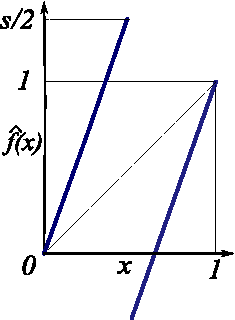
\includegraphics[width=0.30\textwidth]{fig_d_1CL18}
  \caption{\label{fig-d-1f}
$\hflow{}{\ssp}$, the full space sawtooth map \refeq{KD-mapCL18}, ${s} >
2$.
            }
\end{figure}
%%%%%%%%%%%%%%%%%%%%%%%%%%%%%%%%%%%%%%%%%%%%%%%%%%%%%%%%%%%%%%%%%%
%
The closely related {\em sawtooth map}, sketched in \reffig{fig-d-1f},
with `stretching' parameter $s>2$,
\index{sawtooth map}
\beq
\hx_{\zeit+1}
    \,=\, \hflow{}{\hx_{\zeit}}
    \,=\,\left\{
\begin{array}{ll}
{s} \hx_{\zeit}\,,          & \hx_{\zeit} \in [0,{1/2}) \\
{s} \hx_{\zeit} +1 - {s}\,, & \hx_{\zeit} \in ({1/2},1]
\end{array}
\right.
%\,,\qquad {s} \in \{2,3,4, \cdots\}
%\,,
\label{KD-mapCL18}
\eeq

 Since the relation between $\Ssym{\zeit}$ symbol
sequences and $\ssp_{\zeit}$ states is linear, it is straightforward  to
go back and forth between a {\lattstate} and its symbolic
representation.

%%%%%%%%%%%%%%%%%%%%%%%%%%%%%%%%%%%%%%%%%%%%%%%%%%%%%%%%%%%%%
\begin{figure}
  \centering
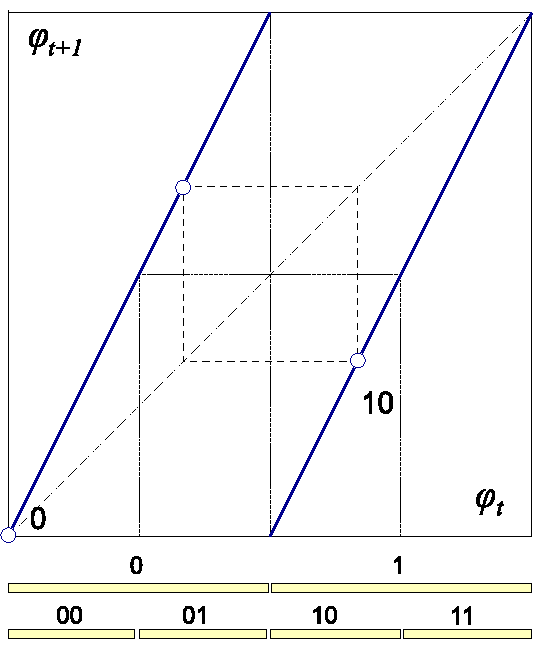
\includegraphics[width=0.35\textwidth]{BernPartKitten}
  \caption{\label{fig:BernPart}
The Bernoulli map \refeq{KD-mapCL18} for ${s}=2$, %{BerShift},
together with the
$\cycle{0}$ fixed point, and the \cycle{01} 2-cycle. Preimages
of the critical point $\ssp_c=1/2$ partition the unit interval into
$\{\pS_0,\pS_1\}$, $\{\pS_{00},\pS_{01},\pS_{10},\pS_{11}\}$, $\dots$,
subintervals.
As the map is a
circle map, $\ssp_{5}=1=0=\ssp_{0} \quad(\mbox{mod}\;1)$.
          }
\end{figure}
%%%%%%%%%%%%%%%%%%%%%%%%%%%%%%%%%%%%%%%%%%%%%%%%%%%%%%%%%%%%%%

The $n$th
preimages $b^{-(n-1)}(\ssp)$ of the critical point $\ssp_c=1/2$
partition the \statesp\ into $2^n$ subintervals, each labeled
by the first $n$ binary digits of points $\ssp=.\Ssym{1}
\Ssym{2} \Ssym{3} \ldots $ within the subinterval:
\reffig{fig:BernPart} illustrates such 4-intervals \statesp\
partition $\{\pS_{00},\pS_{01},\pS_{11},\pS_{10}\}$  for
$\cl{}=2$.

known as the {\em doubling} map if ${s}=2$,
    \index{doubling map}\index{circle map}
\beq
\ssp_{\zeit+1} = 2 \ssp_{\zeit} \;\; (\mbox{mod}\;1)
%    \,,\qquad \qquad \ssp_{\zeit}\in [0,1)
\,,
\ee{DoublingMap}
and {\em ${s}$-tupling} map, \reffig{fig-d-1}\,(b), for
integer stretching parameter ${s}\geq3$,

The relation is linear, and a given \brick\ $\Mm$, or `code' in terms of
alphabet  \refeq{base-sAlph}, corresponds to a unique temporal {\lattstate} $\Xx$ given by the lattice Green's function
\beq
\Xx
= \gd\,\Mm
\,,\qquad
\gd = - \frac{\shift}{\shift - s\,\id}
\,,
\ee{appe:tempBernGreen}
provided we specify the boundary conditions ({\bcs}) for the {\shiftOp}
$\shift$.

The power of the linear encoding of the {temporal
Bernoulli} condition \refeq{1stepDiffEq} is that the
\emph{integer}-valued symbols $\Ssym{\zeit}$ from the finite alphabet
\refeq{base-sAlph} encode the \emph{real-valued} lattice site states
$\ssp_{\zeit}$.

For the  %\rf{GroFuj,art91},
piecewise linear map of \reffig{fig:BernPart}
we can evaluate the \dzeta\ in closed form.
Each branch has the same value of the
slope, and the map can be parameterized
by the single parameter ${s}$.
The larger ${s}$ is, the stronger is the stretching action of the map.

The power of the code % $\{\Ssym{\zeit}\}$
\beq
\transp{\Mm} % = \{\ssp_j\}
             = (\Ssym{\zeit},\Ssym{{\zeit+1}},\cdots,\Ssym{{\zeit+k}})
\ee{linCode}
for the {\templatt} \refeq{OneCat} is that one can use \emph{integers}
$\Ssym{\zeit}$ to encode the \emph{real-valued} {\lattstate}s $\ssp_{\zeit}$.

,
\beq
(\partial - (s-1)\,\shift^{-1})\,\Xx = -\Mm
\,.
\ee{app:1stepVecEq}

For
the $s=3$ cat map example at hand, they are
\beq
\{M_j\} = (M_1,M_2,M_3,M_4,M_5,\cdots)
=(1,2,5,10,24,\cdots)
\,,
\ee{noPrimeCycs=3}

Visualizing the volume relation \refeq{eq:fundFact} for a general \cl{}\dmn\
{\fundPip} is not easy, but

As the {temporal Bernoulli} \refeq{tempBern} is linear, eigenmodes of
$\jMorb$, shifted by $\Mm$ as in \refeq{tempBern} for each distinct
{\lattstate}, are also {\lattstate}s of {temporal Bernoulli}.


    \HLpost{2020-01-17}{
The determinant of this $\jMorb$ from \refeq{tempBern} is negative so
we cannot use the determinant trace formula directly. A correct way is:
first rewrite the $\jMorb$ as in \refeq{appe:tempBernGreen}
\[
\jMorb = \id-{s}{\shift}^{-1}
       = - \frac{s}{\shift} \left(\id-\frac{\shift}{s}\right)
\, .
\]
Note that $\det(\shift)=(-1)^{\cl{}-1}$. The determinant of $\jMorb$ is:
\[
\det \jMorb = \det(\frac{\shift}{s}-\id) s^{\cl{}}(-1)^{\cl{}-1}
   = - s^{\cl{}} \det(\id-\frac{\shift}{s}) \, .
\]
Then use the determinant-trace formula:
\[
\ln\det(\id-\frac{\shift}{s}) = \tr\ln({\id- {\shift}/{s}})
  =
-\sum_{k=1}^\infty\frac{1}{k}\frac{\tr(\shift^k)}{s^k}
\, ,
\]
and use
$\tr \shift^k= \cl{}\delta_{k,\cl{}r}$ if $k$ is a multiple of $\cl{}$,
0 otherwise
(follows from $\shift^\cl{}=\id$),
\[
\ln\det(\id-\frac{\shift}{s}) = -\sum_{r=1}^\infty\frac{1}{r}\frac{1}{s^{\cl{}r}}
=
\ln(1-s^{-\cl{}})
\, ,
\]
and the determinant of $\jMorb$ is:
\[
\det \jMorb = - s^{\cl{}} \det(\id-\frac{\shift}{s}) = 1 - s^{\cl{}}
\, ,
\]
which is negative. So for the {temporal Bernoulli} the count is:
\[
N_\cl{} = |\det \jMorb| = s^{\cl{}} - 1
\, ,
\]
in agreement with the time-evolution count \refeq{noPerPtsBm}.
}

\item[2020-01-25 Predrag:] {\bf A Bernoulli map example}.
%%%%%%%%%%%%%%%%%%%%%%%%%%%%%%%%%%%%%%%%%%%%%%%%%%%%%%%%%%%%%%%%%%%%%%%
% BernCyc2Jacob.svg
% derived from CatMapStatesp.svg
\begin{figure}
  \centering
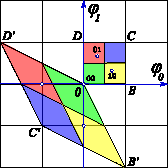
\includegraphics[width=0.45\textwidth]{BernCyc2Jacob}
  \caption{\label{fig:BernCyc2Jacob}
(2020-02-14 Predrag: his is ``wrong'', now superseded with the updated
figure in \refref{CL18}; 2020-09-11 the whole example seems misplaced
here, moce it to wherever it belongs)
The base-2 Bernoulli map \refeq{circ-m=2} period-2 periodic points
$\Xx_p=(\field_0,\field_1)$ are $\cycle{0}=(0,0)$, $\cycle{1}=(1,1)$ fixed
point repeats, and the 2-cycle $\Xx_{01}=({1}/{3},{2}/{3})$,
see \reffig{fig:BernPart}.
They all lie within the unit square $[0BCD]$, one within each
$\pS_{\Ssym{0}\Ssym{1}}$ subregion, and are mapped by the
$[2\!\times\!2]$ {\jacobianOrb} $\jMorb$
% \refeq{jacobianOrb}
into the parallelogram $[0B'C'D']$, whose area is 4 times the unit area.
The images of periodic points $\Xx_p$ land on the integer lattice, and
are sent back into the origin by integer translations $\Mm_p$, in order
to satisfy the fixed point condition
%\refeq{tempBernFix},
$\jMorb\Xx_p+\Mm_p=0$.
          }
\end{figure}
%%%%%%%%%%%%%%%%%%%%%%%%%%%%%%%%%%%%%%%%%%%%%%%%%%%%%%%%%%%%%%
%
The action of {\jacobianOrb}
$\jMorb$ for the period-2 periodic points of the base-2 Bernoulli map,
\reffig{fig:BernPart},
which partitions the unit interval into ${2}$ subintervals
$\{\pS_\Ssym{}\}$, is
\beq
\field_{\zeit+1}
= {2} \field_{\zeit} - \Ssym{\zeit+1}
\,,\qquad  \field_{\zeit}\in\pS_{\Ssym{\zeit}}
\,,
\ee{circ-m=2}
where $\Ssym{\zeit}$ takes values in the ${2}$-letter alphabet
\beq
\Ssym{} \in \A=\{0,1\}
\,.
\ee{base-sAlph=2}

should suffice to convey the idea. In this
case, the $[2\!\times\!2]$ {\jacobianOrb}, the unit
square basis vectors, and their images are
\bea
\jMorb &=&
 \left(\begin{array}{cc}
  1 & -2 \\
 -2 &  1
 \end{array} \right)
;\quad
\Xx_B =
 \left(\begin{array}{c}
 1  \\
 0
 \end{array} \right)
\,,\quad
\Xx_D =
 \left(\begin{array}{c}
 0  \\
 1
 \end{array} \right)
\continue
\Xx_{B'}  &=& \jMorb\,\Xx_B =
 \left(\begin{array}{c}
  1  \\
 -2
 \end{array} \right)
\,,\quad
\Xx_{D'} =
 \left(\begin{array}{c}
-2  \\
 1
 \end{array} \right)
\,,
\eea
with the resulting fundamental parallelogram of area 4
shown in \reffig{fig:BernCyc2Jacob}.
The volume of the fundamental parallelogram lattice $\lattice$ \refeq{lattVol} is
\beq
\Det(\lattice) = \Det(\Xx_{B'}|\Xx_{D'})= \Det(\jMorb)\,\Det(\Xx_{B}|\Xx_{D}) = - 3
\,,
\ee{bernVol}
where in this case the unit cell matrix $(\Xx_{B}|\Xx_{D})=\unit$.


The $[3\!\times\!3]$ {\jacobianOrb} and the unit
cube basis vectors are
\bea
- \jMorb &=&
 \left(\begin{array}{ccc}
  -1  & 0 & 2 \\
  2 &  -1 & 0\\
  0 & 2 & -1
 \end{array} \right)
\,,\quad
\left(\Xx_B|\Xx_C|\Xx_D\right) =
 \left(\begin{array}{ccc}
 1 & 0 & 0\\
 0 & 1 & 0\\
 0 & 0 & 1
 \end{array} \right)
\,.
\nnu
\eea
Clearly $\Det(-\jMorb)= {s}^3-1$, and so on, reproducing the periodic
states count for Bernoulli. No point of looking at $\Det(-\jMorb)$, as
that changes sign at every order - always evaluate $|\Det(\jMorb)|$.

%%%%%%%%%%%%%%%%%%%%%%%%%%%%%%%%%%%%%%%%%%%%%%%%%%%%%%%%%%%%%%%%%%%%%%%
% BernCyc2Jacob.svg
% derived from CatMapStatesp.svg
\begin{figure}
  \centering
{(a)}
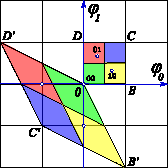
\includegraphics[width=0.35\textwidth]{BernCyc2Jacob}
~~~
{(b)} %$\!\!\!\!$
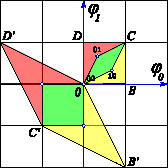
\includegraphics[width=0.35\textwidth]{BernCyc2JacobUnit}
  \caption{\label{fig:BernCyc2JacobOld}
[OLD VERSION] The Bernoulli map \refeq{BerShift} period-2 {\lattstate}s
$\Xx_\Mm=(\ssp_0,\ssp_1)$ are the $\cycle{0}=(0,0)$ fixed
point, and the 2-cycle $\Xx_{01}=({1}/{3},{2}/{3})$, see
\reffig{fig:BernPart}. They all lie within the unit square $[0BCD]$,
one within each $\pS_{\Ssym{0}\Ssym{1}}$ subregion, and are mapped by the
$[2\!\times\!2]$ {\jacobianOrb} $\jMorb$ \refeq{bernFundPar} into the
{\fundPip} $[0B'C'D']$. The images
of periodic points $\Xx_\Mm$ land on the integer lattice, and are sent back
into the origin by integer translations $\Mm$, in order to satisfy the
fixed point condition refeq\{tempFixPoint\}, $\jMorb\Xx_\Mm+\Mm=0$.
\refFig{fig:BernPart} suggests subdividing the {\fundPip}
into (a) 4 areas, but they are not unit areas. The theory of integer lattices
dictates instead (b) covering the {\fundPip} by 3 unit area
rectangles, with
all vertices on the integer lattice.
          }
\end{figure}
%%%%%%%%%%%%%%%%%%%%%%%%%%%%%%%%%%%%%%%%%%%%%%%%%%%%%%%%%%%%%%
%

\PCpost{2020-02-16}{
Dropped from CL18\rf{CL18}:\\
The temporal Bernoulli lattice Green's function %\refeq{appe:tempBernGreen}
in the matrix form
\beq
\gd
=  \left(\begin{array}{ccccccc}
0&\ExpaEig^{-1}&\ExpaEig^{-2}&\ExpaEig^{-3}&\ExpaEig^{-4}&\ExpaEig^{-5}&\cdots\cr
0&  0          & \ExpaEig^{-1}&\ExpaEig^{-2}&\ExpaEig^{-3}&\ExpaEig^{-4}&\cdots\cr
0&  0          &   0          &\ExpaEig^{-1}&\ExpaEig^{-2}&\ExpaEig^{-3}&\cdots\cr
0&  0          &   0          &     0       & \ddots      &  \cr
0&  0          &   0          &     0       & 0           & \ExpaEig^{-1}&\cdots\cr
0&  0          &   0          &     0       & 0           & 0            &\ddots\cr
\vdots&\vdots  &   \vdots     &     \vdots  & \vdots      & \vdots        &\ddots
          \end{array} \right)
\,,
\ee{BernGreenMatrix}
for an infinite temporal Bernoulli
lattice $\zeit\in\integers$, where $\ExpaEig={s}$ is the 1-time step stability
multiplier for the Bernoulli system.
}

\item[2020-02-18 Predrag] Clipped here from
\emph{Ising.tex}, might be relevant to generalizing
Bernoulli to 2\dmn\ lattice, as a warm-up to \catlatt\ zeta functions:

Roettger\rf{Roettger05},
{\em Periodic points classify a family of Markov shifts}, writes:

Ledrappier introduced the following type of space of doubly indexed
sequences over a finite abelian group G,
\[
X_G=\{(x_{s,t}) \in G^{\integers^2} | x_{s,t+1}=x_{s,t}+x_{s+1,t}
\quad \mbox{for all }s,t\in \integers\}.
\]
The group $\integers^2$ acts naturally on the space $X_G$ via left and
upward shifts.

\item[2020-02-19 Predrag]
Suarez\rf{Suarez89}
{\em Difference equations and a principle of double induction},
\CBlibrary{Suarez89}
studies this as a ``partial difference equations,'' that is, difference
equations in two or more variables. He refers to many books on the
subject. His example is a first order hyperbolic equation, with initial
conditions on space and time axes, which describes some thermal
properties,
\[
f(r, m) =f(r, m-1) +f(r-1, m).
%\label{Suarez89(9)}
\]
The goal is to calculate, step by step, all the values of the temperature
T(m,n), starting with the initial and boundary conditions. But then I do
not get the rest of the papers. Perhaps best not to use much time on
`\spt' Bernoulli.

    \item[2020-03-28 Predrag]
The Bernoulli % equation \refeq{circ-m}
first-order difference equation
\beq
\field_{\zeit} - {s}\field_{\zeit-1} = - \Ssym{\zeit}
\,,\qquad  \field_{\zeit} \in [0,1)
\,,
\ee{diffEqs:1stepDiffEq}
{characteristic equation} (for \Ssym{\zeit}=0)
\beq
\ExpaEig -s= 0
\,,
\ee{diffEqs:tempBern}
has one characteristic root
\(
\{s\}
\,.
\)

Comparing with \refeq{genFuncts:noPerPtsBms} we see that we need to solve
a first-order inhomogeneous difference equation with a constant forcing
term $(s-1)$.

Weijie Chen does this pedagogically in his 2011 lecture notes
\CBlibrary{Chen11}, sect.~{\em 1.2.1 One Example}, where he
considers
\beq
\field_{\zeit} - {s}\field_{\zeit-1} = {M}
\,,
\ee{Chen11:1stepDiffEq}
and finds the particular solution by taking
$\field_{p,n} = \field_{p}$ for all $n$,
\[
  \field_{p}-s\,\field_{p}={M}
  \quad \to \quad
  \field_{p} = -{M}/(s-1)
\,.
\]
Hence the solution is
\beq
\field_{n} = \field_{c,n} + \field_{p,n}
= c\,s^{n} - \frac{{M}}{s-1}
\,,
\ee{Chen11:1stepDiffSolu}
with $c$ determined by the initial value
\(
\field_{0}= c\,{s}^{0} - {{M}}/(s-1)
\,.
\)
Bernoulli starts with $\field_{0}=0$, and according to
\refeq{genFuncts:noPerPtsBms}, $M=(s-1)$, so $c=1$.

Weijie Chen also works out the particular solution when $s=1$.
                                    \toCB
He also remarks that in econometrics the {\shiftOp} $\shift$ is called
the \emph{lag operator}.

%\item[2020-03-28 Predrag]
Weijie Chen solves the \templatt\ pedagogically in his lecture notes
\CBlibrary{Chen11}, sect.~{\em 2 Second-Order Difference Equation}.

Questions
\begin{itemize}
  \item
Why is it OK to take site-independent particular solution?
  \item
${{M}}/(s-1)$ looks awkward, can one reformulate? so instead of $M$, have
${{M}}/(s-1)\to1$
  \item
I am guessing that $M=(s-1)$ in \refeq{Chen11:1stepDiffEq}
something like the total number of `letters' I can add to
the count $N_n$ at time $n$. Something like that.
  \item
Similarly for $M=2{\mu}^2$ forcing term in \templatt\ second-order
difference equation \refeq{genFuncts:CatRec-s}.
  \item
This is still just a verification of my guess recurrence
\refeq{genFuncts:noPerPtsBms}.
Make this argument into a derivation.
\end{itemize}

    \PCpost{2020-02-23}{
Just curious - what does the Bernoulli {\fundPip} defined by the columns
of $[3\!\times\!3]$ {\jacobianOrb}
\beq
\jMorb =
\left(
\begin{array}{ccc}
  1 & -2 &  0 \\
  0 &  1 & -2 \\
  -2&  0 &  1
\end{array}
\right)
\,,
\qquad
N_3 = |\Det \jMorb|
    = 2^3-1
\,,
\label{bernFundPar3}
\eeq
look like in a 3\dmn\ rendition? Hopefully it is not symmetric, like
\reffig{fig:catCycJacob}\,(b).
    }

\item[2020-03-01 Predrag]
Wilf\rf{Wilf94} {\em Generatingfunctionology} starts out in his sect.
1.1~{\em An easy 2-term recurrence}, with our Bernoulli periodic points
count \refeq{genFuncts:noPerPtsBm} and
\refeq{genFuncts:1stepDiffEq} as a trivial example of a two-term
recurrence (first-order difference equation).

\item[2020-12-21 Predrag]
{\bf Counting {temporal Bernoulli} {\lattstate}s}
%\label{s:bernCount}
removed from CL18.tex $\to$ Bernoulli.tex, replaced by  refsect{s:Hill1stOrd}
\bigskip

To evaluate the {\HillDet} \refeq{eq:fundFact}, observe that
from \refeq{tempBern} it follows that
\[
\Det(-\jMorb)=\Det({s}/\shift)\,\Det(\id- {\shift}/{s})
\,,
\]
where $|\Det({s}/\shift)|=s^n$. Expand $\ln\Det(\id- {\shift}/{s}) =
\Tr\ln(\id- {\shift}/{s})$ as a series in $1/s$,
\beq
\Tr\ln\left(\id- \frac{\shift}{s}\right)
  =
-\sum_{k=1}^\infty\frac{1}{k}\frac{\Tr(\shift^k)}{s^k}
\,.
\ee{LnDet=TrLn}
It follows from $\shift^\cl{}=\id$ that
$\Tr \shift^k= \cl{}\delta_{k,r\cl{}}$ is non-vanishing
if $k$ is a multiple of $\cl{}$,
0 otherwise:
\[
\ln\Det(\id- {\shift}/{s})
  =
-\sum_{r=1}^\infty\frac{1}{r}\frac{1}{{s}^{\cl{}r}}
  =
\ln(1-{s}^{-\cl{}})
\,.
\]

\item[2020-12-09 Predrag]
{\bf Temporal Bernoulli}
% \label{appe:1D1dLatt}
% was file siminos/kittens/appeBernoulli.tex      pdflatex CL18
%\renewcommand{\statesp}{state space}
%\renewcommand{\Statesp}{State space}
%\renewcommand{\stateDsp}{state-space}
%\renewcommand{\StateDsp}{State-space}
\index{cyclic!permutation matrix}

After $\cl{}$ shifts, the {\lattstate} \Xx\ returns to the initial
state, $\shift^\cl{}=\id$. This relation leads to the explicit expression for
the orbit {\jacobianM} \refeq{appe:tempBernGreen},
\beq
\gd
    =  \frac{\shift}{s\,\id-\shift}
    = \frac{1}{\id-\frac{\shift}{s}}\,\frac{\shift}{s}
    = \sum_{k=1}^\infty \frac{\shift^k}{s^k}
%    =  \sum_{m=0}^\infty \frac{1}{s^{\cl{}m}}
%      \sum_{k=1}^\cl{} \frac{\shift^k}{s^k}
    =  \frac{s^\cl{}}{s^\cl{} - 1}
      \sum_{k=1}^\cl{} \frac{\shift^k}{s^k}
\,.
\ee{appe:BernGreenFct}
From \refeq{appe:tempBernGreen} it then follows that the last field in
$\Xx$ is the field at lattice site $\cl{}$
\beq
\ssp_{\cl{}}
=  \frac{s^\cl{}}{s^\cl{} - 1}
          .\Ssym{1}\Ssym{2}\Ssym{3}\cdots\Ssym{\cl{}}
=  \frac{1}{s - 1}\,%\sum_{k=1}^\cl{} \Ssym{k} 2^{\cl{}-k}
    \frac{s^{\cl{}-1}\Ssym{1}+\cdots+s\,\Ssym{\cl{}-1}+\Ssym{\cl{}}}
         {s^{\cl{}-1}+\cdots+s+1}
\,,
\label{appe:Bern_cyc}
\eeq
and the rest are obtained by cyclic permutations of $\Mm$.

% from ChaosBook \Chapter{appendKnead}
% \section{Pruned Bernoulli shift} \label{sect:PrunBernoulli}
For example, for ${s}=2$, the lattice fields are (they are always rational-valued),
\bea
\ssp_{\Ssym{1}\Ssym{2}\cdots \Ssym{n}}
&=&  \sum_{k=1}^\cl{} \frac{\Ssym{k}}{2^k} \sum_{m=0}^\infty \frac{1}{2^{\cl{}m}}
        = \frac{2^\cl{}}{2^\cl{} - 1} .\Ssym{1}\Ssym{2}\cdots \Ssym{\cl{}}
\continue
&=& \frac{1}{2^\cl{} - 1}\,\sum_{k=1}^\cl{} \Ssym{k} 2^{\cl{}-k}
\,,
\label{Bern_cyc1}
\eea
where $p=\overline{\Ssym{1}\Ssym{2}\cdots \Ssym{\cl{}}}$ is an {\orbit} of period
\cl{}, with stability multiplier $\ExpaEig_p=2^\cl{}$.

For a Bernoulli map,
the rational $\ssp_{0}$ are either periodic or land eventually on a \po\
(the base-${s}$ version of the familiar fact that the decimal expansion
of a rational number is eventually periodic), while the orbit of a normal
irrational $\ssp_{0}$ is ergodic.

    \item[2020-12-09, 2020-12-11 Predrag]
Quotienting the temporal Bernoulli system
\beq
\ssp_{\zeit} - {s}\ssp_{\zeit-1} = - \Ssym{\zeit}
\,,\qquad  \ssp_{\zeit} \in [0,1)
\,,
\ee{1stepDiffEqBlog}
by its \emph{dynamical} $\Dn{1}=\{e,\Refl\}$
symmetry
\beq
\Refl \ssp_\zeit = 1-\ssp_\zeit
    \,,\quad
\Refl \Ssym{\zeit} = (s-1)-\Ssym{\zeit}
    \,,\qquad
\mbox{ for all } \zeit\in\integers
\,,
\ee{BernDynD1}
where $\Ssym{\zeit}$ takes values in the ${s}$-letter alphabet
\beq
\Ssym{} \in \A=\{0,1,2,\cdots,s-1\}
\,.
\ee{base-sAlphBlog}
Define the fundamental domain to be ${\sspRed}_\zeit\in[0,1/2]$.
We construct the
Bernoulli fundamental domain lattice system, with `1/2' unit hypercube
$\hat{\Xx}\in[0,1/2]^\cl{}$, as in
\toChaosBook{exmple.11.3}
{{\em Group \Dn{1} and reduction to the fundamental domain}},
see \reffig{fig:fig_d_2half}\,(b),
and the fundamental domain symbolic dynamics $\hat{\A}$.
The temporal lattice Bernoulli condition \refeq{1stepDiffEqBlog} is now
two conditions  (Bernoulli)/$\Dn{1}$.
They are different for ${s}$ even or odd:
\bea
{\sspRed}_{\zeit+1} - {s} {\sspRed}_{\zeit} &=&
            - \Ssym{\zeit+1}
\,,\qquad  {\sspRed}_{\zeit}\in\pS_{\Ssym{\zeit}}
\,,\quad {s} \mbox{ even}
    \continue
{\sspRed}_{\zeit+1} + {s}{\sspRed}_{\zeit} &=&
       1 + \Ssym{\zeit+1}
\,,\qquad  {\sspRed}_{\zeit}\in\pS_{\Refl\Ssym{\zeit}}
    \label{circ/D1}\\
% \hat{\Ssym{}} \in
\hat{\A}~~~~ &=& \{\{\Ssym{}\},\{\Refl\Ssym{}\}\}
\,,\;\; \{\Ssym{}\} = \{0,1,2,\cdots,{s}/2\}
\,,
\nnu
\eea

\bea
{\sspRed}_{\zeit+1} - {s} {\sspRed}_{\zeit} &=&
\,,\;\;    {s} \mbox{ odd}
\label{base-sRed}\\
%\hat{\Ssym{}} \in
\hat{\A} &=&
\{\{\Ssym{}\},({s}-1)/2,\{\Refl\Ssym{}\}\}
\,,\;\;     \Ssym{}\in \{0,1,2,\cdots,(s-3)/2\}
\,.
\nnu
\eea
As an example, case
${s}=6$,
$\Ssym{\zeit}\in\{0,1,2\}$
is worked out in \reffig{fig:fig_d_2half}\,(c).
(Plot also the fundamental domain map for odd values of ${s}$.)
%
%%%%%%%%%%%%%%%%%%%%%%%%%%%%%%%%%%%%%%%%%%%%%%%%%%%%%%%%%%%%%
\begin{figure}
  \centering
{(a)}
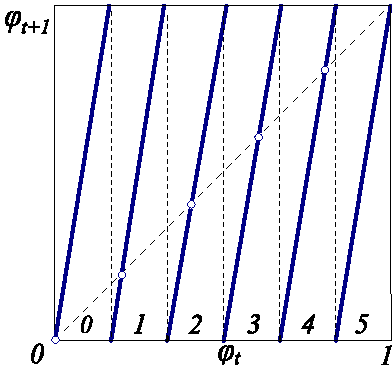
\includegraphics[width=0.40\textwidth]{fig_d_2kitten}
~~~
{(b)}$\!\!\!\!$
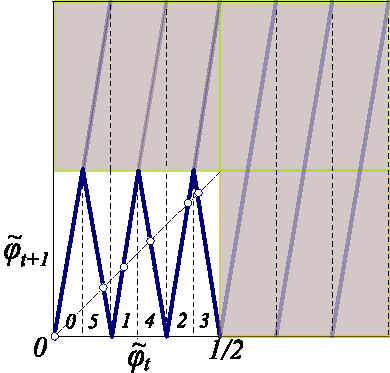
\includegraphics[width=0.40\textwidth]{fig_d_2half}
\\ %~~~
{(c)}$\!\!\!\!$
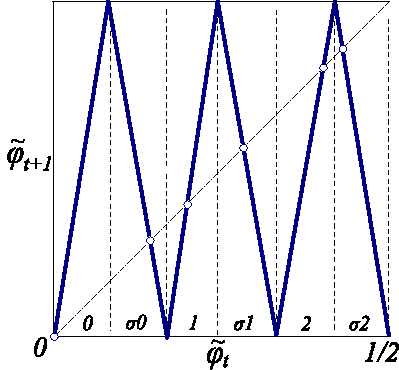
\includegraphics[width=0.40\textwidth]{fig_d_2fund}

  \caption{\label{fig:fig_d_2half}
(a)
The Bernoulli map $f$ with the  stretching parameter ${s}=6$
partitions the unit interval into $6$ subintervals $\{\pS_{\Ssym{}}\}$,
labeled by the ${6}$-letter alphabet \refeq{base-sAlphBlog}. As the map is a
circle map, $\ssp_{5}=1=0=\ssp_{0} \quad(\mbox{mod}\;1)$.
(b)
The Bernoulli map is quotiented by the
\emph{dynamical} $\Group=\Dn{1}=\{e,\Refl\}$
symmetry to
(c)
the fundamental domain ${\sspRed}_\zeit\in[0,1/2]$ map
$\hat{f}=f/\Group$ partitions the half interval into the three $1/12$
subintervals $\{\pS_{0},\pS_{1},\pS_{2}\}$, and their reflections, the
three $3$ subintervals $\{\pS_{\Refl0},\pS_{\Refl1},\pS_{\Refl2}\}$,
labeled by a ${6}$-letter reduced system's alphabet. Reduced space
fixed points $\{\cycle{\Refl_0},\cycle{\Refl_1},\cycle{\Refl_2}\}$
correspond to self-dual 2-cycles
$\{\cycle{05},\cycle{14},\cycle{23}\}$
in the full space. Fixed point $\cycle{0}$ is in the border,
and thus over-counted;
$\cycle{1}$ corresponds to $\{\cycle{1},\cycle{4}\}$, and
$\cycle{2}$ corresponds to $\{\cycle{2},\cycle{3}\}$.
          }
\end{figure}
%%%%%%%%%%%%%%%%%%%%%%%%%%%%%%%%%%%%%%%%%%%%%%%%%%%%%%%%%%%%%%
%

In the matrix form \refeq{1stepDiffEqBlog}, the {\jacobianOrb}
\beq
\jMorb\,\Xx = - \Mm
\,,\qquad
\jMorb = \unit-{s}{\shift}^{-1}
% former \ee{tempBernFix}
\,,
\ee{HLtempBern}
is independent of $\Mm$. Not so for the symmetry reduced  {\jacobianOrb}
${\MvarRed}_{\hat{\Mm}}$ in \refeq{circ/D1}: it depends on
$\hat{\Mm}$, as its diagonal takes values $\pm{s}$. We need to prove
that the \HillDet\ $\Det{\MvarRed}$ does not.

I had not noticed before that this parametrization converts
Bernoulli into tent map, with full \statesp\ 2-cycles turned
into negative slope fixed points.

By the
inclusion-exclusion principle \refeq{KlaRot97(2.1)}
\beq
N_\cl{}=
  \hat{N}_\cl{}+\Refl\hat{N}_\cl{}-\hat{N}_\cl{}\cap(\Refl\hat{N}_\cl{})
      =
  2\hat{N}_\cl{}-\hat{N}_\cl{}\cap(\Refl\hat{N}_\cl{})
\,.
\ee{Bern:inclExcl}
Let's call the number of points in the shared boundary $I$.
% Looks like we have to distinguish odd and even $\cl{}$.
The $\ssp=0$ is in $I$
for any $\cl{}$, if I am allowed to identify $\ssp=1\to0$,
and that is the only point in the boundary.
Presumably this leads to the denominator $(1-z)$ in
\refeq{appe:BernZeta}. I guess that the symmetric irrep of
$\Dn{1}=\{e,\Refl\}$ leads to $N_{+}=s^\cl{}$ and the numerator
$(1-{s}z)$, while the antisymmetric irrep leads to $N_{-}=0$, and a
trivial factor 1 contribution to the numerator \refeq{appe:BernZeta}.
\bea
\zetatop(z)
 &=&
\frac{1 -  {s}z}{1 - z}
\,.
\label{appe:BernZeta}
\eea

\tempLatt\ should be more interesting. Also any nonlinear $s$-branch map
`Bernoulli-like' lattice with a \emph{dynamical} $\Dn{1}$ symmetry; then
the weights $t_p$ do not necessarily cancel for the antisymmetric irrep.

\item[2018-12-27 Linas Vepstas]
{\em On the Beta Transformation} \arXiv{1812.10593}:
The beta transformation is the iterated map \refeq{betaTransf}. The
$\beta=2$ is known as the Bernoulli map, and is exactly solvable. The Bernoulli
map provides a model for pure, unrestrained chaotic (ergodic) behavior:
it is the full invariant shift on the Cantor space. The beta
transformation defines a subshift: iterated on the unit interval, it
singles out a subspace of the Cantor space, in such a way that it is
invariant under the action of the left-shift operator. That is, lopping
off one bit at a time gives back the same subspace. The beta transform
seems to capture something basic about the multiplication of two real
numbers: $\beta$ and $x$. It offers a window into understanding the nature of
multiplication. Iterating on multiplication, one would get
exponentiation; although the mod 1 of the beta transform contorts this in
interesting ways. The work presented here is a research diary: a pastiche
of observations and some shallow insights.
 The eigenvalues of the
transfer operator seem to lie on a circle of radius $1/\beta$ in the complex
plane. Given that the transfer operator is purely real, the appearance of
such a quasi-unitary spectrum seems surprising. The spectrum appears to
be the limit of a dense set of quasi-cyclotomic polynomials, the positive
real roots of which include the Golden and silver ratios, the Pisot
numbers, the n-bonnaci (tribonacci, tetranacci, etc.) numbers.

Beta transformation
\beq
T_{\beta }(x)=\beta x\;{\mod {1}}
\,,\qquad 1<\beta\leq2
\ee{betaTransf}
was introduced by Alfr{\'e}d R{\'e}nyi\rf{Renyi57} in 1957, and an invariant measure for
it was given by Alexander Gelfond in 1959 and independently by Bill
Parry\rf{Parry60} in 1960.

\HREF{https://arxiv.org/pdf/1812.10593.pdf\#subsection.1.9}
{Beta transformation literature review and references}.

\HREF{https://mathoverflow.net/questions/265916/concise-introduction-to-beta-transformations}
{{\em A concise intro to beta-transformations?}} has references.

% A. O. Gel’fand, “A common property of number systems”,
%           Izv Akad Nauk SSSR Ser Mat, 23, 1959, pp. 809–814.

% P. Gaspard, "r-adic one-dimensional maps and the Euler summation
%           formula", Journal of Physics A, 25 (letter) L483-L485 (1992).


\item[2020-09-08 Predrag]
\HREF{https://sites.google.com/site/homepagebingli}{Bing Li}
{\em Some fractal problems in beta-expansions}
\HREF{https://www.irif.fr/~numeration/OWNS}{(video)}
\HREF{https://www.irif.fr/~numeration/uploads/Main/li_20200908.pdf}{(slides)}

For greedy beta-expansions, we study some fractal sets of real numbers
whose orbits under beta-transformation share some common properties. For
example, the partial sum of the greedy beta-expansion converges with the
same order, the orbit is not dense, the orbit is always far from that of
another point etc. The usual tool is to approximate the
beta-transformation dynamical system by Markov subsystems. We also
discuss the similar problems for intermediate beta-expansions.

\item[2021-01-05 Predrag]
Hofbauer and Keller\rf{HofKel84} {\em Zeta-functions and
transfer-operators for piecewise linear transformations} (1984) has no
Bernoulli zeta. Not useful to us at this time.

\item[2021-01-05 Predrag]
Takahashi\rf{Takahashi81} {\em Fredholm determinant of unimodal linear
maps} has lots of detail and examples. I might have missed something, but
Bernoulli zeta is not there, or anything we care about.

\item[2021-01-04 Predrag]
Flatto, Lagarias and Poonen\rf{FlLaPo94}
{\em The zeta function of the beta transformation} (1994)

which should have the $\beta=2$ Bernoulli zeta function
as the trivial case.

\item[2021-01-05 Han] Notes from Flatto, Lagarias and Poonen\rf{FlLaPo94} paper:

$\beta$-transformation map is:
\[
f_\beta(x) = \beta x \;\; (\mbox{mod}\;1) \, ,
\]
where $\beta>1$, $x \in [0,1]$. The symbolic dynamics of $f_\beta$ is based on the fact that the graph of
$f_\beta$ consists of $\lfloor \beta \rfloor + 1$ monotone pieces which they call laps, which are
assigned by the symbols $0, 1, \dots, \lfloor \beta \rfloor$. When $\beta \in \mathbb{Z}^+$,
the piece $\lfloor \beta \rfloor$ consists of a single point, and the symbol $\lfloor \beta \rfloor$
only appears in the itinerary of 1. To each $x \in [1,0]$ its itinerary is $I_\beta(x)=A_0A_1A_2\dots$,
where the symbol
\[
A_n := A_n(x) = \lfloor \beta f_\beta^n(x) \rfloor \, .
\]
In particular the itinerary of 1, $I_\beta(1)=A^*_0A^*_1A^*_2\dots$ encodes complete information about
the behavior of $f_\beta$.

They introduced a power series with integer coefficients:
\[
\phi_\beta(z) = A_0^* z + A_1^* z^2 + A_2^* z^3+ \dots = \sum_{n=0}^{\infty} A_n^* z^{n+1} \, .
\]
This function is related to the iterates of 1 by:
\[
\phi_\beta(z) = 1 + (\beta z - 1)\left(
\sum_{n=0}^\infty f_\beta^n(1)z^n
\right)
\, .
\]
Then the zeta function is:
\[
\zeta_\beta(z) = \frac{1}{1-\phi_\beta(z)} \, ,
\]
if $\beta$ is not a simple $\beta$-number, and
\[
\zeta_\beta(z) = \frac{1-z^N}{1-\phi_\beta(z)} \, ,
\]
if $\beta$ is a simple $\beta$-number, and $N$ is minimal with $f_\beta^N(1)=0$.
Simple $\beta$-numbers are the $\beta$-numbers such that for some $n$, $f_\beta^n(1)=0$.
This formula gives the correct topological zeta function of temporal Bernoulli.

Associated with the $\beta$-transformation is the set $X_\beta$ of all $I_\beta(x)$ for $0 \leq x <1$.
The $\beta$-shift $S_\beta$ is a symbolic dynamical system obtained as the smallest closed (two-sided)
subshift of $\{1,2,\dots \lfloor \beta \rfloor\}^{\mathbb{Z}}$ generated by all finite substrings of $X_\beta$.
For simple $\beta$-numbers $S_\beta$ is a subshift of finite type.

There is a zeta function associated to the $\beta$-shift $S_\beta$, which is studied by
Takahashi\rf{Takahashi83}, who showed that
\[
\hat{\zeta}_\beta(z) = \frac{1}{1-\phi_\beta(z)} \, .
\]
This formula is closely related to $\zeta_\beta(z)$ but differs from it for simple $\beta$-numbers,
in which case the closure operation defining $S_\beta$ adds some extra periodic points.

\item[2021-01-11 Predrag] Seth Lloyd \etal. %\rf{LDGKLMTP20}
{\em Quantum algorithm for nonlinear differential equations}
\arXiv{2011.06571}:

[1] showed how to map the problem of solving a general linear differential
equation to that of matrix inversion, which can then be performed using
the quantum linear systems algorithm [12-13].   Consider a linear differential
equation of the form,
$$ {dx\over dt} + A x = b(t), \eqno(6)$$
where as above $x,b \in {\cal C}^d$ and $A$ is a $[d\times d]$ matrix.

                                                            \toCB
Discretize the equation in time at intervals $\Delta t$, and take $k$ to
be the index for the discretized time, so that $x_k$ and $b_k$ are
the values of $x$ and $b$ at time label $k$.

We wish to integrate equation
(6) numerically starting from the initial state $x_0 \equiv b_0$.   We obtain
a series of equations of the form:
$$
 x_0 = b_0 \quad
x_1 = x_0 - \Delta t A x_0 + \Delta t b_1 \quad
\ldots \quad
x_{k+1} = x_k - \Delta t A x_k + \Delta t  b_k \quad
\ldots
\eqno(7)$$
Here, we have used the Euler forward method for numerical integration, but it
is straightforward to implement implicit methods such as
Euler backward, Crank-Nicholson, Runge-Kutta, etc.~[3].
Written in matrix form, these equations become
$$-\left(\begin{array}{cccccc}
- I & 0 & 0 & \ldots & 0 & 0 \cr
I-\Delta t A & - I & 0 & \ldots & 0 & 0 \cr
0 & I-\Delta t A& -I &  \ldots & 0 & 0\cr
&&\ldots &&&\cr
0& 0 & 0 & \ldots & - I & 0\cr
0& 0 & 0 & \ldots & I - \Delta t A & - I\cr
          \end{array} \right)
\left(\begin{array}{c}
x_0 \cr x_1 \cr x_2 \cr \ldots \cr x_{T-1} \cr x_{T}
          \end{array} \right)
=
\left(\begin{array}{c}
b_0 \cr \Delta t b_1 \cr \Delta t b_2 \cr \ldots \cr \Delta t
b_{T-1} \cr \Delta t b_{T}
          \end{array} \right)
%\eqno(8)
\,,
$$







\end{description}

%%%%%%%%%%%%%%%%%%%%%%%%%%%%%%%%%%%%%%%%%%%%%%%%%%%%%%%%%%%%%%%%%%%%%%%%%%%%%
\Remarks
%%%%%%%%%%%%%%%%%%%%%%%%%%%%%%%%%%%%%%%%%%%%%%%%
% PC 2021-01-04 eventually merge into
% \Chapter{appendStatM}{22jun2016}{Statistical mechanics applications}
\remark{Bernoulli map.}{\label{rem:Bernoulli}
The Bernoulli shift map \refeq{BerShift} and the doubling map
\refeq{DoublingMap} are also known as the dyadic transformation, dyadic
map, bit shift map, angle doubling map or sawtooth map \refeq{KD-map}.
There are many fine books that discuss it in depth, for example Driebe\rf{Driebe99}.
See also \refrem{rem-GroRue}.
\index{Bernoulli!shift}\index{shift!Bernoulli}
\index{doubling map}\index{circle map}
\index{dyadic transformation}\index{dyadic map}
\index{bit shift map}\index{angle doubling map}
\index{sawtooth map}
    } %end \remark{rem:Bernoulli}
%%%%%%%%%%%%%%%%%%%%%%%%%%%%%%%%%%%%%%%%%%%%%%%%

%%%%%%%%%%%%%%%%%%%%%%%%%%%%%%%%%%%%%%%%%%%%%%%%
% PC 2021-01-04 eventually merge into
% \Chapter{converg}{9nov2008}{Why does it work?}
\remark{Bernoulli shift.}{ \label{rem-GroRue}
For a more in-depth discussion, consult chapter~3 of \refref{Driebe99}.
The extension of Fredholm theory to the case of Bernoulli shift on
$\complex^{k+\alpha}$ (in which the \FPoper\ is {\em not} compact  --
technically it is only {\em quasi-compact}. That is, the essential
spectral radius is strictly smaller than the spectral radius) has been
given by Ruelle\rf{Ruelle90}: a concise and readable statement of the
results is contained in \refref{Baladi95}. We see from \refeq{mixing-BS}
that for the Bernoulli shift the exponential decay rate of correlations
coincides with the Lyapunov exponent: while such an identity holds for a
number of systems, it is by no means a general result, and there exist
explicit counterexamples.
See also \refrem{rem:Bernoulli}.
\index{Bernoulli!shift}\index{shift!Bernoulli}
} %end \remark{Bernoulli shift on $C^{k+\alpha}$}{
%%%%%%%%%%%%%%%%%%%%%%%%%%%%%%%%%%%%%%%%%%%%%%%%

\RemarksEnd

%%%%%%%%%%%%%%%%%%%%%%%%%%%%%%%%%%%%%%%%%%%%%%%%%%%%%%%%%%%%%
\fastTrackExam{exam:BernShad}     % \toExam
%%%%%%%%%%%%%%%%%%%%%%%%%%%%%%%%%%%%%%%%%%%%%%%%%%%%%%%%%%%%%

    \ifboyscout\clearpage\fi
% siminos/kittens/cat.tex      pdflatex CL18
% $Author: predrag $ $Date: 2021-07-29 00:36:31 -0400 (Thu, 29 Jul 2021) $

\section{A kicked rotor}
\label{s:kickRot}

    \PC{2021-07-24}{
Most of this material moved to LC21; skip and/or abbreviate.
    }


The 1-degree of freedom maps that describe kicked rotors
subject to discrete time sequences of angle-dependent impulses
$P(\coord_{\zeit})$, $\zeit\in\integers$,
\bea
\coord_{\zeit+1} - \coord_{\zeit} &=& p_{\zeit+1} \qquad  (\mbox{mod}\;1),
    \label{PerViv2.1b}\\
p_{\zeit+1} - p_{\zeit} &=& P(\coord_{\zeit})
\,,
    \label{PerViv2.1a}
\eea
with $2\pi \coord$ the  angle of the rotor, $p$ the momentum conjugate to
the angular coordinate $\coord$, and the angular pulse
$P(\coord)=P(\coord+1)$ periodic with period $1$, play a key role in the
theory of classical and quantum chaos in  atomic physics, from the
Taylor, Chirikov and Greene  standard map\rf{Lichtenberg92,Chirikov79},
to the cat maps discussed below. The equations are of the canonical
Hamiltonian form: \refeq{PerViv2.1b} is $\dot{\coord}=p/m$ in terms of
discrete time derivative \refeq{lattTimeDer}, \ie, the configuration
trajectory starting at $\coord_{\zeit}$ reaches
$\coord_{\zeit+1}=\coord_{\zeit}+p_{\zeit+1}\Delta{\zeit}/m$ in one time
step $\Delta{\zeit}$, and \refeq{PerViv2.1a} is the time-discretized
$\dot{p}=-\partial V(\coord)/\partial \coord$: at each kick the angular
momentum $p_{\zeit}$ is accelerated to $p_{\zeit+1}$ by the force pulse
$P(\coord_{\zeit})\Delta{\zeit}$, with the time step set to
$\Delta{\zeit}=1$, and the rotor mass $m$ set to 1.

For an atomic physics kicked rotor, the values of the angle $\coord$
differing by integers are identified, but the momentum $p$ is unbounded.
As for the Bernoulli map \refeq{BerStretch}, one compactifies the
momentum by adding $(\mbox{mod}\;1)$ to \refeq{PerViv2.1a}. This reduces
the phase space to a square $[0,1)\times [0,1)$ of unit area, with the
opposite edges identified.

%\section{Life of a single Hamiltonian cat}
\subsection{Cat map}
%    \fi
\label{s:catPV}

The simplest kicked rotor is subject to a force is proportional to
displacement, that is, Hooke's law force $P(\coord)=K\coord$ linear in
the angular displacement $\coord$. The $(\mbox{mod}\;1)$ added to
\refeq{PerViv2.1a} makes the map a discontinuous `sawtooth,' unless $K$
is an integer. In the integer $K$ case, the map
(\ref{PerViv2.1b},\ref{PerViv2.1a}) is of form
 \beq
 \left(\begin{array}{c}
 \coord_{\zeit+1}  \\
   p_{\zeit+1}
  \end{array} \right )=
  \jMat \left(\begin{array}{c}
 \coord_{\zeit}  \\
   p_{\zeit}
  \end{array} \right )\quad (\mbox{mod}\;1)
    \,,  \qquad
 {\jMat} =\left(\begin{array}{cc}
 a & c \\
 d & b
  \end{array} \right)
\,,
\ee{catMap}
where $a,b,c,d$ are integers whose precise values do not matter, as long
as $\det \jMat=1$, \ie, the map is area-preserving. The map is then a
Continuous Automorphism of the Torus, or a {\em `cat map'}, a linear
area-preserving map on the unit 2-torus \statesp, with the field at the
temporal lattice site \zeit,
\(
\ssp_{\zeit} =(\coord_{\zeit},p_{\zeit}) \in  (0,1]\times(0,1]
\)
interpreted as the angular position and its conjugate momentum
at time instant $\zeit$.
    \PC{2020-02-20}{
A matrix $\jMat$  is called hyperbolic when it has no eigenvalue on the unit circle.
    }

We consider the case of stability multipliers
$(\ExpaEig\,,\;\ExpaEig^{-1})$ real, with a positive Lyapunov exponent
$\Lyap >0$,
\beq
\ExpaEig=e^{\Lyap}=(s+\sqrt{(s-2)(s+2)})/2
\,,\qquad
s=\tr{\jMat}=\ExpaEig+\ExpaEig^{-1}
\,.
\ee{StabMtlpr}
The eigenvalues are functions of the single stretching parameter $s$, and
for $|s| > 2$ the cat map \refeq{catMap} is a fully chaotic
Hamiltonian dynamical system. Cat maps with the same $s$ are equivalent
up to a similarity transformation, so it suffices to work out a single
convenient realization, as we shall do here for the \PV\ example
\refeq{eq:StateSpCatMap}.

Cat maps are beloved by ergodicists and statistical mechanicians because,
even though the field $(\coord_{\zeit},p_{\zeit})$ is 2\dmn, for integer
values of the stretching parameter $s$, a cat map has a finite alphabet
linear code, just like the Bernoulli map, and its
unit torus can be tiled by two rectangles,
    \PC{2020-12-17}{
Link to the ChaosBook.
    }
in analogy with the forward-in-time Bernoulli map subinterval
partitioning of \reffig{fig:BernPart}. From this it follows that all
admissible symbol {\brick}s can be generated as shifts of finite
type, and all periodic points determined and counted.

As all that is well known, and a side issue for this paper, we relegate
the details of the Hamiltonian cat map dynamics and \po\ counting to
??.
    \PC{2020-12-17}{
Link to the ChaosBook.
    }
Here we focus on reformulating the cat dynamics as
a temporal lattice (or discrete Lagrangian) problem, as we have done for
the Bernoulli system in \refsect{s:1D1dLatt}.

\subsection{\tempLatt}
\label{s:catLagrange}
    % earlier names:
    % \section{Life of a single Lagrangian cat}
    % \section{Cat map in Lagrangian formulation}
\renewcommand{\period}[1]{{\ensuremath{n_{#1}}}}
    % discrete length of a cycle, Predrag

To motivate our formulation of a \spt\ chaotic field theory to be
developed in \refsect{s:catlatt}, we again recast the local initial
value, time-evolution cat \emph{map} \refeq{catMap} as a global
\emph{temporal lattice} condition that we shall refer to as the
{\em \templatt}.

The discrete time Hamilton's equations
(\ref{PerViv2.1b},\ref{PerViv2.1a}) induce forward-in-time evolution on a
2-torus  $(\coord_{\zeit},p_\zeit)$ {\em phase space}. For the problem at
hand, it pays to go from the Hamiltonian (configuration, momentum) phase
space formulation to the discrete Lagrangian
$(\ssp_{\zeit-1},\ssp_{\zeit})$ formulation. If the momentum is replaced
by the discrete time velocity,
\beq
(\coord_\zeit,p_\zeit) \to
\left(
    \ssp_{\zeit},\frac{\ssp_{\zeit} - \ssp_{\zeit-1}}{\Delta\zeit}
\right)
%\,,\qquad \Delta\zeit= 1
\,,
\ee{Ham2Lagr}
and the time step set to $\Delta\zeit=1$, a cat map can be brought to the
\PV\ `two-configuration representation'\rf{PerViv}
\beq
 \left(\begin{array}{c}
 \ssp_{\zeit}  \\
 \ssp_{\zeit+1}
 \end{array} \right )=
 \jMat_{PV} \left(\begin{array}{c}
 \ssp_{\zeit-1}  \\
 \ssp_{\zeit}
 \end{array} \right ) %\mbox{ mod } 1
 - \left(\begin{array}{c}
 0  \\
 \Ssym{\zeit}
 \end{array} \right )
 \,,  \qquad
 {\jMat_{PV}} =\left(\begin{array}{cc}
 0 & 1 \\
 -1 & s
 \end{array} \right ),
%\,.
\ee{eq:StateSpCatMap}
with matrix $\jMat_{PV}$ acting on the 2\dmn\ space of successive
configuration points $\transp{(\ssp_{\zeit-1},\ssp_{\zeit})}$. As was
case for the Bernoulli map \refeq{1stepDiffEq}, the cat map
$(\mbox{mod}\;1)$ condition \refeq{catMap} is enforced by integers
$\Ssym{\zeit}\in  \A$, where for a given integer stretching parameter $s$
the alphabet \A\ ranges over $|\A|={s}\!+\!1$ possible values for
$\Ssym{\zeit}$,
\beq
\A=\{\underline{1},0,\dots s\!-\!1\}
\,,
\ee{catAlphabet}
necessary  to keep $\ssp_{\zeit}$ for all times $t$ within the unit
interval $[0,1)$. We find it convenient to have symbol
$\underline{\Ssym{}}{}_{\zeit}$ denote $\Ssym{\zeit}$ with the negative
sign, \ie, `$\underline{1}$' stands for symbol `$-1$'. As for the
Bernoulli system, $\Ssym{\zeit}$ can be interpreted as `winding
numbers'\rf{Keating91}, or, as they shepherd stray points back into the
unit torus, as `stabilising impulses'\rf{PerViv}. Here we shall refer to
them as a `code', or, in the field-theoretical parlance, as `sources'.

Written out as a second-order difference equation, the \PV\ map
\refeq{eq:StateSpCatMap} takes a particularly elegant, {\em \templatt}
form
\beq
\ssp_{\zeit+1}  -  s \, \ssp_{\zeit} + \ssp_{\zeit-1}
    =
-\Ssym{\zeit}
\,,
\ee{catMapNewt}
or,
in terms of a {lattice state} $\Xx$, the corresponding {symbol \brick}
$\Mm$ \refeq{pathBern}, and the $[\cl{}\!\times\!\cl{}]$ {\shiftOp}
$\hopMat$ \refeq{hopMatrix},
\beq
(\hopMat - s\id + \hopMat^{-1})\,\Xx = -\Mm
\,,
\ee{catTempLatt}
very much like the {temporal Bernoulli} condition \refeq{tempBern}.
`Temporal' again refers to the global lattice state (field) $\Xx$, and
the winding numbers (sources) $\Mm$ taking their values on the lattice
sites of a 1\dmn\ \emph{temporal} lattice $\zeit\in\integers$.

For a finite lattice segment $\Xx$, one needs to specify the boundary
conditions ({\bcs}).
%  for the Green's function \refeq{tempCatGreen}.
The companion article \refref{GHJSC16} tackles the Dirichlet {\bcs}, a
difficult, time-translation symmetry breaking, and from the \po\ theory
perspective, a wholly unnecessary, self-inflicted pain. All that one
needs to solve the {\templatt} are the $\period{}$-periodic,
time-translation invariant {\bcs} used here.
    \PC{2020-02-08}{
Complain about that stupidity clearly both in the intro and in conclusions.
    }


\subsection{\JacobianOrb}
\label{s:tempCatJacobianOrb}

Again, the {temporal lattice} reformulation gives us a different perspective
into how to enumerate and determine global solutions of such systems. The
{\templatt} condition \refeq{catTempLatt} can be viewed as a search for
zeros \refeq{tempFixPoint} of the function
\beq
F[\Xx] = \jMorb\Xx+\Mm = 0
\,,
\ee{tempCatFixPoint}
% refer to \ee{tempFixPoint}
with the entire periodic \emph{lattice state} ${\Xx}_{\Mm}$ treated as a
single fixed \emph{point} $(\ssp_1,\ssp_{2},\cdots,\ssp_{\cl{}})$ in the
\cl{}\dmn\ \statesp\ unit hyper-cube $\Xx\in[0,1)^\cl{}$, where
the $[\cl{}\!\times\!\cl{}]$ {\jacobianOrb} $\jMorb$ is now given by
\beq
\jMorb = \hopMat - s\id + \hopMat^{-1}
% \,.
\ee{tempCatFix}
a tri-diagonal Toeplitz matrix (constant along each diagonal,
$\jMorb_{k\ell} = j_{k-\ell}$) of circulant form,
\beq
\jMorb %  = \hopMat - s\id + \hopMat^{-1}
  =
\left(\begin{array}{ccccccc}
 -{s}& 1 & 0 & 0 &\dots &0& 1 \\
 1 &  -{s}& 1 & 0 &\dots &0&0 \\
0 & 1 &  -{s}& 1 &\dots &0 & 0 \\
\vdots & \vdots &\vdots & \vdots & \ddots &\vdots &\vdots\\
0 & 0 & \dots &\dots &\dots  & -{s}& 1 \\
 1 & 0 & \dots &  \dots &\dots& 1 &  -{s}
        \end{array} \right)
\,.
\ee{Hessian}

% PC 2020-07-24 turned the former
% \subsection{Hill's formula:
%           stability of an orbit vs. its time-evolution stability}
% \label{s:tempLattHill}
% (that was here) into a separate section Hill.tex

\subsection{Fundamental fact} %{Integer lattices}
\label{s:catIntLat}

As in \refsect{s:bernIntLat}, the {\fundPip} given the stretching of the
\cl{}\dmn\ \statesp\ unit hyper-cube $\Xx\in[0,1)^\cl{}$ by the {\jacobianOrb}
counts periodic lattice states, with the {\admissible} lattice states of
period $\period{}$ constrained to field values within
$0\leq\ssp_\zeit<1$. The {\fundPip} contains images of all periodic
lattice states $\Xx_\Mm$, which are then translated by integer winding
numbers $\Mm$ into the origin, in order to satisfy the fixed point
condition \refeq{tempCatFixPoint}. The total number of periodic lattice
states is again, as for the Bernoulli system \refeq{detBern0}, given by
the `fundamental fact'
\beq
N_\cl{} = |\Det\jMorb|
\,.
\ee{detCat0}

Period-1, or fixed point lattice states are easy to count: the
{\jacobianOrb} is a 1\dmn\ matrix, so it follows from
\refeq{catMapNewt} that
\beq
N_1={s}-2
\,,
\ee{catFundPar1}
        \PC{2020-06-10}{to Han:
    If the alphabet \refeq{catAlphabet} is really $|\A|={s}\!+\!1$
    letters, how come there are only ${s}-2$ fixed point lattice states?
    Where did the extra 3 letters go?
        }
        \HL{2020-06-12}{
        The fixed point lattice states with the other 3 letters are not admissible. The fixed point solution satisfies:
        \[
        ({s}-2)\ssp_\zeit = \Ssym{\zeit} \, .
        \]
        Since $\ssp_\zeit \in [0,1)$, the range of \Ssym{\zeit} is $\Ssym{\zeit} \in [0,s-2)$. So the letter $\underline{1}$, $s-2$ and $s-1$ are not in the admissible range, as the corresponding fields of these 3 letters are $-1/(s-2)$, $1$ and $(s-1)/(s-2)$ respectively.
        }

%%%%%%%%%%%%%%%%%%%%%%%%%%%%%%%%%%%%%%%%%%%%%%%%%%%%%%%%%%%%%
% Predrag 2020-02-08 replaced Han's
% {HLLength2Counting}.pdf by hand-drawn catCyc2Jacob.svg
% Han & PC 2020-02-11
% siminos/figSrc/han/Mathematica/CountingFigure/HLLength3Counting.nb
\begin{figure}
  \centering
(a)~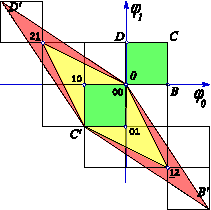
\includegraphics[width=0.38\textwidth]{catCyc2JacobUnit}
~~~
(b)~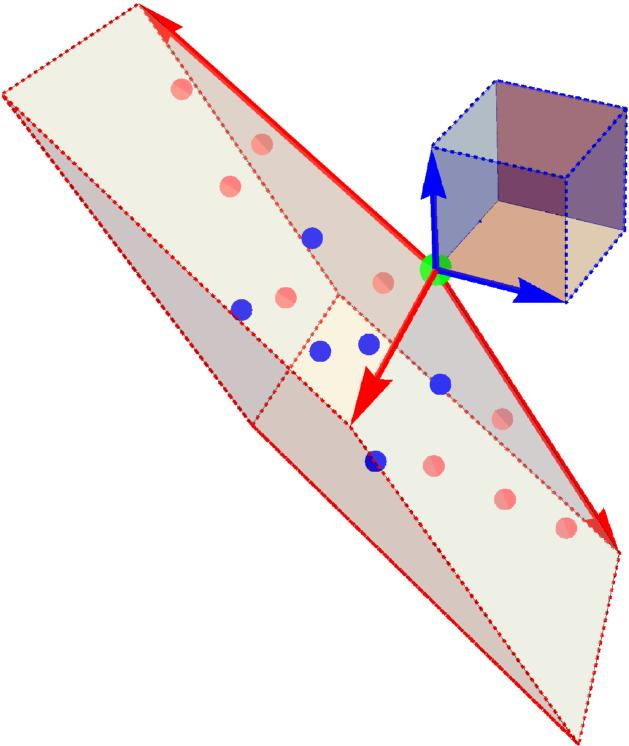
\includegraphics[width=0.34\textwidth]{PCLength3Counting}
  \caption{\label{fig:catCycJacob}
(a)
    For $s=3$, the \templatt\ \refeq{catTempLatt} has 5 period-2 lattice
    states $\Xx_\Mm=(\ssp_0,\ssp_1)$: $\Xx_{00}$ fixed point and
    2-cycles $\{\Xx_{01},\Xx_{10}\}$,
    $\{\Xx_{\underline{1}2},\Xx_{2\underline{1}}\}$. They lie
    within the unit square $[0BCD]$, and are mapped by the
    $[2\!\times\!2]$ {\jacobianOrb} $\jMorb$ \refeq{catFundPar2} into the
    {\fundPip} $[0B'C'D']$, as in, for example, Bernoulli
    \reffig{fig:BernCyc2Jacob}. The images of periodic points $\Xx_\Mm$
    land on the integer lattice, and are sent back into the origin by
    integer translations $\Mm= \Ssym{0}\Ssym{1}$, in order to satisfy the
    fixed point condition
    %\refeq{tempCatFixPoint},
    $\jMorb\Xx_\Mm+\Mm=0$.
(b) A 3-dimensional [{\color{blue} blue} basis vectors] unit-cube stretched by
    $\jMorb$ \refeq{catFundPar3} into the [{\color{red} red} basis vectors]
    {\fundPip}. For $s=3$, the \templatt\
    \refeq{catTempLatt} has 16 period-3 lattice states: a $\Xx_{000}$
    fixed point at the vertex at the origin, [{\color{red} pink dots}] 3
    period-3 orbits on the faces of the {\fundPip}, and
    [{\color{blue} blue dots}] 2 period-3 orbits in its interior.
    An \cl{}\dmn\ \statesp\ unit hyper-cube $\Xx\in[0,1)^\cl{}$ and the
    corresponding {\fundPip} are half-open, as indicated
    by dashed lines, so the integer lattice points on the far corners, edges
    and faces do not belong to it.
}
\end{figure}
%%%%%%%%%%%%%%%%%%%%%%%%%%%%%%%%%%%%%%%%%%%%%%%%%%%%%%%%%%%%%%%

The action of the \templatt\ {\jacobianOrb} can be hard to visualize,
as a period-2 lattice state is a 2-torus,
period-3 lattice state a 3-torus, \etc. Still, the {\fundPip} for the period-2
and period-3 lattice states, \reffig{fig:catCycJacob}, should suffice to
convey the idea. The {\fundPip} basis vectors %\refeq{lattJac}
are the
columns of $\jMorb$. The $[2\!\times\!2]$ {\jacobianOrb} \refeq{Hessian}
and its {\HillDet} are
\beq
\jMorb =
 \left(\begin{array}{cc}
 -s &  2 \\
  2 & -s
 \end{array} \right)
\,,\qquad
N_2=\Det\jMorb=({s}-2)({s}+2)
\,,
\ee{catFundPar2}
(compare with the lattice states count
\refeq{1stChebGenF}),
with the resulting {\fundPip} shown in \reffig{fig:catCycJacob}\,(a).
Period-3
lattice states for $s=3$ are contained in the half-open {\fundPip} of
\reffig{fig:catCycJacob}\,(b), defined by the columns of $[3\!\times\!3]$
{\jacobianOrb}
\beq
\jMorb =
\left(
\begin{array}{ccc}
-{s}&  1 &  1 \\
  1 &-{s}&  1 \\
  1 &  1 &-{s}
\end{array}
\right)
\,,
\qquad
N_3 = |\Det \jMorb|
%   = {s}^3-3{s}-2
    = ({s}-2)({s}+1)^2
\,,
\label{catFundPar3}
\eeq
again in agreement with the periodic orbit count \refeq{1stChebGenF}.

The 16 period-3 lattice
states $\Xx_\Mm=(\ssp_0,\ssp_1,\ssp_3)$ are the $\Xx_{000}$ fixed point at the
vertex at the origin, 3 period-3 orbits
on the faces of the {\fundPip}, and 2 period-3 orbits in its
interior, all five of form
    $\{
       \Xx_{\Ssym{0}\Ssym{1}\Ssym{2}},
       \Xx_{\Ssym{1}\Ssym{2}\Ssym{0}}
       \Xx_{\Ssym{2}\Ssym{0}\Ssym{1}}
    \}$
.

Note that in the {temporal lattice} reformulation, the \templatt\
happens to involve two unrelated lattices:
\begin{itemize}
  \item[(i)]
In the latticization of a time continuum, one replaces a time-dependent
field $\ssp(\zeit)$ at time $\zeit\in\reals$ of \emph{any} dynamical system by a
discrete set of its values $\ssp_\zeit=\ssp(\zeit\Delta{T})$,
$\zeit\in\integers$. Here the index $`\zeit'$ is a \emph{coordinate} over
which the field $\ssp$ lives.
  \item[(ii)]
A peculiarity of the \templatt\ is that the \emph{field} $\ssp_{\zeit}$
\refeq{eq:StateSpCatMap} is confined to the unit interval $[0,1)$,
imparting a $\integers^1$ lattice structure onto the calculationally
intermediate {\fundPip} $\jMorb$ basis vectors \refeq{lattJac}.
\end{itemize}


\subsection{Counting \templatt\ lattice states (unwritten)}
\label{s:tempCatCount}

We now count the number of periodic lattice states \refeq{noPerPts} in
the \templatt\ (or, `discrete Lagrangian') formulation (for counting
using the Hamiltonian formulation, see [...]
    \PC{2020-12-17}{
Link to the ChaosBook.
    }


[...]
one can write
the {\HillDet} compactly as
\beq
N_\period{} = |\det(\jMorb)|
 = 2\,T_{\period{}}(s/2) -2
% = \ExpaEig^{\period{}} + \ExpaEig^{-\period{}} - 2
\,,
\label{POsChebyshev}
\eeq
where $T_{\period{}}(s/2)$ is the Chebyshev polynomial of the first kind.
% end of copied from siminos/spatiotemp/chapter/Green1d.tex

\subsection{Counting \templatt\ lattice states (experimental)}
\label{s:tempCatCountTEMP}
% 2020-06-10 Predrag

The \templatt\ equation \refeq{catMapNewt} is
a linear {$2$nd-order inhomogeneous difference} equation
($3$-term recurrence relation) with constant coefficients
%\beq
%\ssp_{\zeit+1}  -  s \, \ssp_{\zeit} + \ssp_{\zeit-1}
%    =
%-\Ssym{\zeit}
%%\,.
%\ee{eq:CatMapNewton2}
that can be solved by standard methods\rf{Elaydi05} that
parallel the theory of linear differential equations.
    \PC{2020-06-10}{
    Comparing with \refeq{genFuncts:CatRec-s} we see that we need to
    solve a second-order inhomogeneous difference equation with a
    constant forcing term $2\,(s-2)$.
    }
Inserting a solution of form $\ssp_{\zeit}=\ExpaEig^\zeit$ into the
associated (\Ssym{\zeit}=0) homogenous {$2$nd-order difference equation}
\beq
\ssp_{\zeit+1} - {s}\,\ssp_{\zeit} + \ssp_{\zeit-1}= 0
\ee{diffEqs:CatCharEq}
yields the {characteristic equation}
\beq
\ExpaEig^{2} - {s}\ExpaEig + 1 = 0
\,,
\ee{diffEqs:StabMtlpr}
which, for $|s|>2$, has two real roots
% stability multipliers
$\{\ExpaEig\,,\;\ExpaEig^{-1}\}$,
\beq
\ExpaEig
=\frac{1}{2}(s+\sqrt{(s-2)(s+2)})
\,,
\ee{PCStabMtlpr}
and the so-called \emph{complementary} solution of form
\beq
\ssp_{c,\zeit}  = a_1\ExpaEig^\zeit+a_{-1}\ExpaEig^{-\zeit}
\,.
\label{PC(2.3.4)}
\eeq
% where constants $a_i$ can be determined by specifying
% $\{\ssp_{0},\ssp_{1}\}$.

A difference of any pair of solutions to the \templatt\
inhomogenous equation \refeq{catMapNewt}
%\beq
%\ssp_{\zeit+1} - {s}\,\ssp_{\zeit} + \ssp_{\zeit-1}= -\Ssym{\zeit}
%%\,,
%\ee{PC(2.4.4)}
is a solution of the homogenous difference equation
\refeq{diffEqs:CatCharEq}, so the general solution is a sum of the
{complementary} solution \refeq{PC(2.3.4)} and a \emph{particular}
solution $\ssp_{p}$,
\beq
\ssp_{\zeit} = \ssp_{c,\zeit} + \ssp_{p,\zeit}
\,.
\ee{PC(2.4.3)}
Eq.~\refeq{diffEqs:CatCharEq} is time-reversal invariant,
$\ssp_{\zeit} = \ssp_{-\zeit}$, so $a_1=a_{-1}=a$.
To determine the particular solution, assume that both the source
 $\Ssym{\zeit}=\Ssym{}$
and $\ssp_{p,\zeit}=\ssp_{p}$
 in \refeq{catMapNewt} are site-independent,
\beq
\ssp_{p}  -  s \,\ssp_{p} + \ssp_{p}
    = -\Ssym{}
\,,
\ee{eq:CatMapNewton5}
so
\(
%  2\,\ssp_{p}-s\,\ssp_{p}={M}
%  \quad \to \quad
  \ssp_{p} = \Ssym{}/(s-2)
\,.
\)
Hence the solution is
\beq
\ssp_{\zeit} = \ssp_{c,\zeit} + \ssp_{p,\zeit}
= a\left(\ExpaEig^{\zeit} + \ExpaEig^{-\zeit}\right) + {\Ssym{}}/(s-2)
\,,
\ee{Chen11:1stepDiffSolu}
with $a_i$ determined by fields at two lattice sites,
\[
\ssp_{0}= 2a + {\Ssym{}}/(s-2)
\,,\quad
\ssp_{1}= a\left(\ExpaEig + \ExpaEig^{-1}\right) + {\Ssym{}}/(s-2)
\,,\quad
\,.
\]
\tempLatt\ starts with $N_{0}=0$, and according to \refeq{catFundPar1},
$N_{1}=s-2$, so $a=1$, $\Ssym{}=-2(s-2)$, and the number
of temporal lattice states of period $\cl{}$ is
\beq
N_{\cl{}} =
    \ExpaEig^{\cl{}} + \ExpaEig^{-\cl{}} - 2
\,.
\ee{PC:1stepDiffSolu}

\subsection{Shadowing}
\label{s:tempCatShadow}

As the
relation between the symbol {\brick}s $\Mm$  and the corresponding
lattice states $\Xx_\Mm$ is linear, for $\Mm$ an {\admissible} symbol
\brick, the corresponding lattice state $\Xx_\Mm$ is given by
the Green's function
\beq
\Xx_\Mm
= \gd\,\Mm
\,,\qquad
\gd = \frac{1}{-\hopMat + s\id - \hopMat^{-1}}
\,,
\ee{tempCatGreen}
as in the Bernoulli case \refeq{tempBernGreen}.

As in \refsect{s:bernShadow}, the Green's function \refeq{tempCatGreen}
decays exponentially  with the distance from the origin, a fact that is
essential in establishing the `shadowing' between lattice states sharing
a common sub-\brick\ \Mm. For an infinite temporal lattice
$\zeit\in\integers$, the lattice field at site $\zeit$ is determined by
the sources $\Ssym{\zeit'}$ at all sites ${\zeit'}$, by the  Green's function
$g_{\zeit\zeit'}$ for one\dmn\ discretized heat
equation\rf{PerViv,varcyc},
\beq
  \ssp_{\zeit}=\sum_{\zeit'=-\infty}^\infty g_{\zeit\zeit'} \Ssym{\zeit'}
\,, \qquad
%  g_{\zeit\zeit'} =
%       \left(\frac{1}{-\Box -2 +s}\right)_{\zeit\zeit'}
g_{\zeit\zeit'}=\frac{1}{\ExpaEig-\ExpaEig^{-1}}\,
                \frac{1}{\ExpaEig^{|\zeit-\zeit'|}}
% \,,\qquad
% s=\ExpaEig+\ExpaEig^{-1}
\,,
\ee{1dLatGreenFct}  %{Coord}
with $\ExpaEig$ is the expanding stability
multiplier defined in \refeq{StabMtlpr}.

Suppose there is a non-vanishing point source $\Ssym{0}\neq0$ only at the
present, $\zeit'=0$ temporal lattice site. Its contribution to
$\ssp_{\zeit}$ $\sim \ExpaEig^{-|\zeit|}$ decays exponentially  with the
distance from the origin. More generally, as in the Bernoulli case
\refeq{Bern_cyc}, if two lattice states $\Xx$, $\Xx'$ share a common
sub-\brick\ \Mm\ of length \cl{}, they shadow each other with accuracy of
order of $O(1/\ExpaEig^{\cl{}})$.

\subsection{\Tzeta}
\label{s:tempCatZeta}

The number of lattice states of period $\cl{}$ is
given by the area of the {\fundPip} \refeq{detCat0}
(Hill's formula)
%\rf{Isola90,Keating91}
\beq
N_{\cl{}} = |\Det\jMorb|
          = |\det(\jMat^{\cl{}} - \id)|
          = \ExpaEig^{\cl{}} + \ExpaEig^{-\cl{}} - 2
\,,
\ee{noPerPts}
where the $\ExpaEig$ is the stability multiplier \refeq{StabMtlpr} of the
one-time-step evolution matrix $\jMat$ \refeq{catMap}.
         \PC{2021-07-28}{
Jaidee, Moss and Ward\rf{JaMoWa19},
{\em Time-changes preserving zeta functions}, say that
a Lehmer–Pierce sequence\rf{Lehmer33,Pierce1916}, with $n$th term
\(
|\det(A^n - I)|
\)
for some integer matrix
$A$, counts periodic points for an ergodic toral endomorphism if it is non-zero
for all $n \geq 1$.
    }

Substituting the numbers of lattice states $N_{\cl{}}$ into the {\em
{\tzeta}} \refeq{topoZeta} we obtain
\index{topological!zeta function}
\index{zeta function!topological}
\index{Artin-Mazur zeta function}
\index{zeta function!Artin-Mazur}
\bea
\zetatop(z)
 &=& \exp \left(-\sum_{\cl{}=1}^\infty
\frac{z^\cl{}}{\cl{}} N_\cl{}
         \right)
 =  \exp \left(-\sum_{\cl{}=1}^\infty
\frac{z^\cl{}}{\cl{}} (\ExpaEig^\cl{} + \ExpaEig^{-\cl{}} - 2)
         \right)
\continue
 &=&
\exp \left[\ln(1 - z \ExpaEig) + \ln(1 - z \ExpaEig^{-1}) - 2 \ln(1 - z) \right]
\continue
 &=&
\frac{(1 - z \ExpaEig)(1 - z \ExpaEig^{-1})}{(1 - z)^2}
 =
\frac{1 - s z + z^2}
     {(1 - z)^2}
\,,
\label{Isola90-13}
\eea
in agreement with Isola\rf{Isola90}, as well as the \AW\ generating
partition \tzeta\ \refeq{Isola90-13a}. \Tzeta s count {\em prime
orbits}, \ie, time invariant \emph{sets} of equivalent lattice states
related by translations (cyclic permutations), and other
symmetries\rf{CBcount}.

Conversely, given the \tzeta, the generating function for the number of
temporal lattice states of period $\cl{}$ is given by the logarithmic
derivative of the {\tzeta} \refeq{zetatop-N},
\bea
\sum_{{n}=0}^\infty N_{n} z^{n}
    & = & \frac{2-{s}z}{1 - s z + z^2}-\frac{2}{1 - z}
    \continue
& = & (s-2)\left[z + ({s}+2) z^2 + ({s}+1)^2 z^3 \right.
    \ceq
      \left.\qquad\quad
      +\,({s}+2)\,{s}^2 z^4 + (s^2+ s-1)^2 z^5  +  \cdots\right]
\,,
\label{1stChebGenF}
\eea
which is indeed the generating function for $T_{\period{}}(s/2)$, the
Chebyshev polynomial of the first kind \refeq{POsChebyshev}. The
numbers of {periodic points} and \emph{prime} cycles $M_n$ (given by
\refeq{primeCount}) are in agreement with the Bird and Vivaldi\rf{BirViv}
census, see \reftab{tab:catMapN_n-s=3}.

%%%%%%%%%%%%%%%%%%%%%%%%%%%%%%%%%%%%%%%%%%%%%%%%%%%%
\begin{table}
\begin{tabular}{c|rrrrr|rrrrr|rrrrr}
$n$ &  1 &  2 &  3 &  4 &  5 &
       6 &  7 &  8 &  9 & 10 &
      11 \\%& 12 & 13 & 14 & 15 \\
\hline
$N_n$ &   1 &   5 &  16 &  45 &  121 &
        320 & 841 & 2205 &5776 &15125&
       39601& %   &      &     & 1364
             \rule[-1ex]{0ex}{3.5ex} \\
$M_n$ &   1 &   2 &   5 &  10 &   24 &
         50 & 120 & 270 & 640 & 1500 &
       3600 &  %% &     &     &
\end{tabular}
\bigskip
\caption{\label{tab:catMapN_n-s=3}
Lattice states and {prime} orbit counts for the ${s}=3$ cat map.
}
\end{table}
%%%%%%%%%%%%%%%%%%%%%%%%%%%%%%%%%%%%%%%%%%%%%%%%%%%%
                               \toCB

\subsection{\tempLatt\ as a continuous time dynamical system}
\label{s:tempCatODE}

Recall how the Bernoulli first-order difference equation could be viewed as
a time-discretization of the first-order linear ODE \refeq{1stepVecEq}. The
second-order difference equation \refeq{catMapNewt} can be interpreted as the
second order discrete time derivative ${d^2}/{dt^2}$, or the temporal
lattice Laplacian,
\beq
\Box \, \ssp_\zeit \equiv
\ssp_{\zeit+1} - 2\ssp_{\zeit} + \ssp_{\zeit-1}
= (s-2)\ssp_{\zeit} -\Ssym{\zeit}
\,,
\ee{PerViv2.2}
 with the time step set to $\Delta\zeit=1$.
But that is nothing but Newton's Second Law: ``acceleration equals
force,'' so Percival and Vivaldi\rf{PerViv} refer to this formulation as
`Newtonian', while Allroth\rf{Allroth83}, Mackay, Meiss, Percival, Kook
\& Dullin\rf{meiss92,MacMei83,MKMP84,DulMei98,kooknewt}, and Li and
Tomsovic\rf{LiTom17b} refer  to it as the `Lagrangian' formulation.
%, \refsect{s:catLagrForm}.

In other words, for a cat map the force pulse $P(\coord)=(s-2)\,\coord$
in \refeq{PerViv2.1a} is linear in the angular displacement $\coord$, so
the temporal lattice equation takes form
\beq
(-\Box + (s-2)\id)\,\Xx = \Mm
%    \,,  \qquad
% \Box\,\ssp_{\zeit}:= \ssp_{\zeit-1}-2\ssp_{\zeit} +\ssp_{\zeit+1}
\,.
\ee{OneCat}
For small stretching parameter values, $s<2$, this equation describes a
set of coupled penduli, with oscillatory solutions, known as the
discrete Helmholtz equation or the tight-binding model, with
Hamiltonian\rf{Economou06}
\[ %beq
H=\sum_\ell\ket{\ell}\epsilon_0\bra{\ell}
  + \sum_{\ell m}\ket{\ell}V_{\ell m}\bra{m}
\,,\quad
   V_{\ell m} = \left\{
     \begin{array}{ll}
         V & \mbox{if\ } \ell,m \mbox{ nearest neighbors}\\
         0 & \mbox{otherwise}
     \end{array}
             \right.
\] %ee{Economou06(5.7)}
corresponding to the stretching factor ${s}=-\epsilon_0/V$ in
eq.~\refeq{OneCat}.

Here we study the strong stretching, $s>2$ case, known as the discrete
{\em \sPe} (hyperbolic, damped solutions)\rf{Dorr70,FetWal03,Pozrikidis14}. We
refer to eq.~\refeq{OneCat} as the `{\em \templatt}', both
to distinguish it from the forward-in-time Hamiltonian cat \emph{map}
\refeq{catMap}, and in the anticipation of the \catlatt\ of
\refsect{s:catlatt}.

\bigskip

\noindent\textbf{\tempLatt, summarized.}
In the \spt\ formulation a \emph{global} {temporal lattice state}
\beq
\transp{\Xx} % = \{\ssp_j\}
             = (\ssp_\zeit,\ssp_{\zeit+1},\cdots,\ssp_{\zeit+k})
\ee{path}
is not determined by a forward-in-time `cat map' evolution
\refeq{catMap}, but rather by the fixed point requirement
\refeq{tempCatFixPoint} that the \emph{local}, 3-term discrete temporal
lattice condition \refeq{catMapNewt} is satisfied at every lattice
point. The Lagrangian formulation requires only temporal lattice states
and their actions, replacing the phase space `cat map' \refeq{catMap}
by a `{\templatt}' lattice \refeq{OneCat}. The {\templatt} has no
generating partition analogue of the \AW\ partition for a Hamiltonian cat
map (see
    \PC{2020-12-17}{
Link to the ChaosBook.
    }
).
As we have shown here, no funky Hamiltonian \statesp\ partitioning magic
(such as
    \PC{2020-12-17}{
Link to the ChaosBook.
    }
) is needed to count the periodic
lattice states of a \templatt. Not only are no such partitions needed to
solve the system, but the Lagrangian, temporal 1\dmn\ lattice formulation
is the bridge that takes us from the single cat map \refeq{catMap} to
the higher-\dmn\ coupled infinity ``multi-cat'' \spt\ lattices
\refeq{dDCatsT}.

And did you know that the cute Arnold cat is but the % very fundamental
{\sPe} in disguise?


\renewcommand{\period}[1]{{\ensuremath{T_{#1}}}}         %continuous cycle period


%\renewcommand{\Ssym}[1]{{\ensuremath{m_{#1}}}}
\renewcommand{\statesp}{state space}
\renewcommand{\Statesp}{State space}
\renewcommand{\stateDsp}{state-space}
\renewcommand{\StateDsp}{State-space}

    \ifboyscout\clearpage\fi
% siminos/kittens/catlatt.tex      pdflatex CL18
% $Author: predrag $ $Date: 2021-07-17 21:31:44 -0400 (Sat, 17 Jul 2021) $

\section{\catLatt} % {Herding cats}  %
\label{s:catlatt}


The \emph{\templatt} of \refsect{s:kickRot}  is a 1\dmn\ example of the simplest
{\spt}ly chaotic, or `turbulent' field theory, the {\em \catlatt} to
which we turn now. \catLatt\ lives on a  $d$\dmn\ discretized spacetime,
a {\spt} $\integers^d$ integer lattice, with a cat map (a `rotor') on
each site, coupled to its nearest neighbors. Another way of visualizing a
\catlatt\ is as a lattice of locally hyperbolic `anti' oscillators, as
opposed to the classical free field theory, with an oscillator at each
site (`Gaussian model'\rf{Kadanoff00,Fradkin13}).

The \templatt\ lives on a $1$\dmn\ temporal integer lattice $\integers$,
with very  simple `tilings'. For every integer temporal period
$\period{}$, we first determine $N_\period{}$, the number of all periodic
\emph{lattice state} ${\Xx}_{\Mm}$ solutions on a tile of length
$\period{}$. However, if $\period{}=m\period{p}$, the $\period{}$-tile
can be tiled by $m$ repeats of a smaller  $\period{p}$-tile, so {some} of
$\period{}$-{\po} {solutions} are repeats of the already determined
shorter $\period{p}$ \emph{prime} solution  $\Xx_p$. Furthermore, due to
the time invariance of the defining equations, there are $\period{p}$
physically equivalent copies of a given solution in the time orbit of
every $\Xx_p$. So all we really have to do is to enumerate $M_\period{}$
{\em prime orbits} of the time-invariance equivalent \po\ solutions,
whose generating function is the analytically elegant {\tzeta}.

For the $d$\dmn\ \catlatt\ the repertoire of periodic tilings is richer.
In $d=2$ and $3$ the basic facts are well known both from
crystallography, and from the number theory of integer lattices. In this
paper we systematically construct and enumerate distinct $d=2$ tilings,
or Bravais lattices $\LTS{}{}{}$, of increasing spacetime periodicities,
and determine $N_{\LTS{}{}{}}$, the number of \emph{doubly periodic
lattice state} solutions, by evaluating the associated {\HillDet}s.
For $d=2$ and higher-dimensional lattices
counting the \spt\ `prime' tilings requires some thought. We
determine $M_{\LTS{}{}{}}$, the numbers of
doubly-periodic prime orbits, invariant under spacetime translations.
% In this paper we do not quotient the $\integers^2$ space group point, or
% discrete symmetries, and
We, however, fail to find an analytic form for the associated
doubly-periodic {\tzeta}.

We start by a
brief review of physical origin of coupled map lattices (CMLs) models.
The impatient reader should proceed directly to the
{\catlatt}, introduced in \refsect{s:catLatt}, and solved in
\refsect{s:catLattCount}.

\subsection{Coupled map lattices}
\label{s:CCMs}

In order to solve a partial differential equation (PDE) on a computer,
one represents it by a finite number
of computational elements. The simplest discretization of a scalar
spacetime field $\ssp(\vec{q},\tau)$ is by specifying its values
$\ssp_{n_1n_2\cdots{n_{d-1}}\zeit}= \ssp(q_n,\tau_t)$ on lattice points
$(\vec{n},t) \in \integers^{d}$. Once spatial and temporal derivatives
are replaced by their discretizations, the PDE is
reduced to dynamics of a coupled map lattice, a spatially extended system
with discrete time, discrete space, and a set of continuous fields
on each site. For many PDEs, CML conceptual advantage is not only numerical,
but also that the technical problems such as existence and uniqueness of
the field theory are regularized away, and the essence of {\spt} chaos is
revealed in a transparent form.

Often one starts out by coupling neighbors harmonically, and
thinks of this starting, free field theory formulation as a spring
mattress\rf{Zee10} to which  weakly coupled nonlinear terms are then
added. Similarly, the conventional CML models, mostly motivated by
discretizations of dissipative PDEs, start out with chaotic on-site
dynamics weakly coupled to neighboring sites, with a strong space-time
asymmetry. An example are the diffusive coupled map lattices introduced by
Kaneko\rf{Kaneko83,Kaneko84}, with time evolution given by
\bea
\ssp_{n, t+1}
    &=&     (1+\epsilon\,\Box) g(\ssp_{n\zeit})
           \continue
    &=&    g(\ssp_{n\zeit}) + \epsilon %\,\frac{1}{2}
            [
            g(\ssp_{n-1,t}) - 2g(\ssp_{n\zeit}) + g(\ssp_{n+1,t})
            ]
\,,
\label{KanekoCML}
\eea
where the individual spatial site's dynamical system $g(x)$ is a 1\dmn\
map, such as the logistic map, coupled to its nearest neighbors by
$\Box$, the spatial version of the Laplacian \refeq{PerViv2.2} for the
discretized second order \emph{spatial} derivative ${d^2}/{dx^2}$ (we
always set the lattice spacing constant equal to unity).

The form of time-step map $g(\ssp_{n\zeit})$ is the same for all times, \ie, the
law of temporal evolution is invariant under the group of  discrete
\emph{time translations}.
Spatially homogenous lattice models also invariant under discrete \emph{space
translations} were studied by Bunimovich and Sinai\rf{BunSin88} in the case
when  $g(\ssp_{n\zeit})$  is a one\dmn\ expanding map.

The observation that for {\spt}ly chaotic systems space and time should
be considered on the same footing goes back to the `chronotopic' program
of Politi and collaborators\rf{LePoTo96, LePoTo97, PoToLe98, GiLePo95}
who, in their studies of propagation of {\spt} disturbances in extended
systems, discovered that the spatial stability analysis can be combined
with the temporal stability analysis, with orbit weights depending
exponentially both on the space and the time variables,
$t_p\propto{e^{-\speriod{}\period{}\lambda_p}}$.
Politi and
Torcini\rf{PolTor92} study of \twots\ of \emph{\spt\ H{\'e}non}, a
(1+1)-spacetime lattice of H{\'e}non maps with solutions periodic
both in space and time is the closest to the present investigation.
They explain why the dependence
of the lattice field at time $\ssp_{t + 1}$ on the two previous time
steps prevents an interpretation of dynamics as the composition of a
local chaotic evolution with a diffusion process \refeq{KanekoCML}.
In the CML tradition, they study the weak coupling regime $\epsilon\approx0$, but note that the
$b=-1$ case could be an interesting example of a nonlinear Hamiltonian
lattice field theory.


\subsection{Hamiltonian coupled map lattices}
\label{s:HCCMs}

For quantum
mechanics and statistical mechanics applications, one needs the dynamics to
be Hamiltonian, motivating models such as coupled standard map
lattice\rf{KanGra87} and
% Hoover and Aoki
$\phi^4$ lattice\rf{HooAok16}.
%,AokKus00a,AokKus00b,HuLiZh00,AokKus02,AokKus03}
%
Lattice recurrence relations\rf{MraRin12} of the type studied below arise
in the Frenkel-Kontorova lattice, Hamiltonian lattice models for
ferromagnetism, many-body quantum chaos\rf{SieRic01,MuHeBrHaAl04,
GutOsi13a,GutOsi13,GutOsi15}, and in discretizations of elliptic PDEs.
% 2019-06-26  Mramor and Rink
%{\em Ghost circles in lattice {Aubry-Mather} theory}, \arXiv{1111.5963}:
% 2016-10-27 Boris:
% M. Sieber and K. Richter\rf{SieRic01},
% S. M\"uller, S. Heusler, P. Braun, F. Haake and A. Altland\rf{MuHeBrHaAl04},
% Gutkin and Osipov\rf{GutOsi13a}, Gutkin and Osipov\rf{GutOsi13}


Pesin and Sinai\rf{PesSin88} were the first to study such lattices, with
chains of coupled Anosov maps.
In order to establish rigorously the desired statistical
properties of coupled map lattices, such as the continuity of their {SRB}
measures, they, and most of the subsequent statistical mechanics literature,
relied on the structural stability of Anosov automorphisms under small
perturbations. For such lattices the neighboring sites have to be coupled
sufficiently weakly (small $\epsilon$ in \refeq{KanekoCML}) so that the site
cat maps could be conjugated to a lattice of uncoupled Anosov automorphisms,
with a finite Markov partition, the key ingredient required for the proofs.

This exploration, as well as the companion paper\rf{GHJSC16} for
Dirichlet \bcs, starts with the study of a coupled $\speriod{}$-body
Hamiltonian system undertaken by Gutkin and Osipov\rf{GutOsi15}. If the
reader wants to quantize an $\speriod{}$-body Hamiltonian system, Gutkin and Osipov
article covers the formalism in depth, so we do not review the
Hamiltonian formulation here.

\subsection{\catLatt}
\label{s:catLatt}

In their paper, Gutkin and Osipov also note that if the single `body'
dynamics is described by a cat map coupled to its nearest spatial
neighbors, and if the spatial coupling strength is taken to be the same
as temporal coupling strength, one obtains a {\spt}ly symmetric 5-term
recurrence relation
\beq
       \ssp_{n,\zeit+1} + \ssp_{n,\zeit-1}
- 2{s} \, \ssp_{n\zeit}
     + \ssp_{n+1,\zeit} + \ssp_{n-1, \zeit}
     = -\Ssym{n\zeit}
\,,
\ee{CatMap2d}
that adds one spatial lattice direction to  the {\templatt} 3-term
recurrence relation \refeq{catMapNewt}. As these equations are
symmetric under interchange of the `space' and the `time' directions,
their temporal and spatial dynamics are strongly coupled, corresponding to $\epsilon
\approx O(1)$ in \refeq{KanekoCML}, in contrast to the traditional
spatially weakly coupled CML\rf{BunSin88}.

Now that we have mastered the {\em \templatt} \refeq{catMapNewt}, a
generalization to the {\em \catlatt} \refeq{CatMap2d} is
immediate. Consider a 1\dmn\ spatial lattice, with field $\ssp_{n\zeit}$
(the angle of a kicked rotor \refeq{PerViv2.1b} at instant $\zeit$) at
\spt\ site $z=(n,\zeit)\in\integers^2$. If each site couples only to its
nearest spatial neighbors $\ssp_{n\pm1,\zeit}$, and if we require
(1) invariance under spatial translations,
(2) invariance under spatial reflections, and
(3) invariance under the space-time exchange,
we arrive at the 2\dmn\ Euclidean lattice difference equations
\refeq{CatMap2d}.

Gutkin and Osipov --for reasons that make sense in context of $\speriod{}$-body
quantum systems-- call this recurrence relation a `non-perturbed coupled
cat map'. A well-established name\rf{Dorr70,FetWal03} for this system is
the `discrete {\sPe}'. We, however, find a `\emph{\catlatt}' more descriptive
for our field-theoretic purposes.
While the generalization of \refeq{CatMap2d} to $d$\dmn\ hypercubic
$\integers^d$ lattice is immediate, it suffices to work out the $d=2$
\catlatt\ in some detail to develop intuition about the general case.

The \catlatt\ equation \refeq{CatMap2d} can
be written compactly as
\beq
\jMorb\,\Xx =-\Mm
\,,\qquad
\jMorb = \hopMat_1+\hopMat_{2}-2{s}\id+\hopMat_{2}^{-1}+\hopMat_{1}^{-1}
\,,
\ee{catLatt}
where $\hopMat_1, \hopMat_2$ are {\shiftOp}s \refeq{hopMatrix} which
translate the field by one lattice spacing in the spatial, temporal
direction, respectively. The inverses $\hopMat_{i}^{-1}$ translate the
field in the opposite directions.
The \brick\ $\Mm=\{\Ssym{n\zeit}\}$ is composed of symbols from alphabet
\beq
\Ssym{n\zeit}\in\A
\,,\qquad
 \A  =
 \{\underline{3},\underline{2},\underline{1},0,\cdots,2{s}\!-\!2,2{s}\!-\!1\}
\,,
\label{catLatt2d}
\eeq
where symbol $\underline{\Ssym{}}{}_{n\zeit}$ denotes $\Ssym{n\zeit}$ with the
negative sign, \ie, `$\underline{3}$' stands for symbol `$-3$'.
%
In our explicit computational examples, we shall always set ${s}$ to
\beq
{s}=5/2
    \quad\Rightarrow\quad
 \A  =
 \{\underline{3},\underline{2},\underline{1},0,1,2,3,4\}
\,,
\ee{s=5over2}
the smallest value of the `stretching' parameter $s$ for which the
{\jacobianOrb} $\jMorb$ is an integer-valued matrix, and  the system is
hyperbolic.

%Building upon the $d=1$ {\templatt} developed in \refsect{s:catLagrange},

As for the {temporal Bernoulli} \refeq{tempBern} and the
\templatt\ \refeq{tempCatFixPoint}, one can view the
\catlatt\ condition
\refeq{catLatt} as a zero of the function
\beq
F[\Xx] = \jMorb\Xx+\Mm = 0
\,,
\ee{lattFixPoint}
with the entire periodic {lattice state} ${\Xx}_{\Mm}=\{\ssp_z\}$ treated
as a single fixed {point} within the $(\ell_1\ell_2\cdots\ell_d)$\dmn\
\statesp\ unit hyper-cube $\Xx\in[0,1)^{\ell_1\ell_2\cdots\ell_d}$, where $\ell_j$
is the lattice period in direction $j$, and the
$(\ell_1\ell_2\cdots\ell_d)^2$\dmn\ {\jacobianOrb} $\jMorb_{zz'}$ is
given by
\beq
\jMorb = \sum_{j=1}^{d}\left(\hopMat_j-{s}\id+\hopMat_{j}^{-1}\right)
\,.
\ee{catlattFix}
Here $\hopMat_i$ is a {\shiftOp}
\refeq{hopMatrix} which translates the field in the $i$th
direction by one lattice spacing. Its inverse $\hopMat_{i}^{-1}$
translates the field in the negative $i$th direction.

In multi-index, or `tensorial' notation, the \catlatt\ equation
\refeq{catLatt} can be written as
\bea
\left(\jMorb\ssp\right)_{{z}}
&=&
\sum_{{z}'} \sum_{i=1}^{d} \left(
\hopMat_{i}-{s}\id+\hopMat_{i}^{-1}
                               \right)_{{z}{z}'}
     \ssp_{{z}'} = - \Ssym{z}
\,,\quad
  \Ssym{z} \in \A
\,,
\continue
&& \,{z} \;=\, (n_1,n_2,n_3,\cdots,n_d) \in \integers^d
\continue
&& \A \,=\, \{-2d+1, -2d+2,\cdots,2{s}-2,2{s}-1\}
\,,
\label{dDCatsT}
\eea
with field $\ssp_{z}$ and source $\Ssym{z}$ labelled by the $d$ indices
of lattice site $z$.  Sources $\Ssym{z}\in\A$ keep the field (`rotor
angle' $\ssp_{z}$) within the unit interval on every site. The
{\jacobianOrb} $\jMorb$, labelled by $d$ pairs of indices, acts on the
lattice state \Xx\ by usual matrix multiplication. We illustrate how that
works by working out  in detail an example in \refappe{s:catLattRel3x2}.
As yet another notational choice,  in \refeq{catalattLxT} we recast
the \jacobianOrb\ \refeq{catLatt} as a
$[\speriod{}\period{}\times\speriod{}\period{}]$ Kronecker product block
matrix.

In the {lattice} formulation, the \catlatt\
happens to involve two quite distinct lattices:
\begin{itemize}
  \item[(i)]
In the latticization of a spacetime continuum, one replaces a
time-dependent field $\ssp(x,\zeit)$ at spacetime point
$(x,\zeit)\in\reals^d$ of \emph{any} field theory by a discrete set of
its values $\ssp_z=\ssp(n\Delta{L},\zeit\Delta{T})$  on lattice sites,
where the index $z\in\integers^d$ is a discrete $d$\dmn\
spacetime \emph{coordinate} over which the field $\ssp$ lives.
We describe the properties of this integer
lattice $\integers^d$ and its sublattices in
\refsecttosect{s:lattSymm}{s:primeLatt}.
  \item[(ii)]
A peculiarity of the \catlatt\ is that the \emph{field} $\ssp_{z}$
\refeq{CatMap2d} is confined to the unit interval $[0,1)$, imparting a
$\integers^1$ lattice structure --in any spacetime dimension $d$-- onto
the calculationally intermediate {\fundPip} $\jMorb$ basis vectors (see,
for example, \refeq{3times2basisVecs}).
The lattice structure of \twots\ \Xx\ is discussed in
\refsecttosect{s:lattState}{s:Hill}.
\end{itemize}



%2020-09-05
\subsection{Symmetries of the integer lattice}
\label{s:lattSymm}

The \catlatt\ equation \refeq{catLatt} is \emph{equi}variant under
the discrete spacetime translations;
the space $\sigma_{x}$ and time $\sigma_{y}$ reflections $n\to -n$,
$t\to-t$;
as well as under $\sigma_{a}$ exchange $n\longleftrightarrow t$ of space
and time.
{\catLatt} thus has the point-group symmetries of the square lattice:
rotations by $\pi/2$, and reflection across $x$-axis, $y$-axis, and
diagonals $a$ and $b$,
\beq
C_{4v} = \Dn{4} = \{
E, C_{4z}^+, C_{4z}^-, C_{2z},
\sigma_{y}, \sigma_{x},
\sigma_{a},\sigma_{b},
\}
\,.
\ee{eq:C4v}
In the international crystallographic notation, the square lattice space
group of symmetries is referred to as $p4mm$\rf{Dresselhaus07}.

\newpage %TEMPORARY
\subsection{Sublattices}
\label{s:BravaisLatt}

For the 1\dmn\ temporal lattices considered so far,
a sublattice is tiled by repeats of a \brick\ of temporal period \period{}.

    \PCedit{ %2020-09-05
For a $d$\dmn\ integer lattice $\integers^d$, a $d$-periodic
sublattice that tiles the spacetime is called a
\emph{Bravais lattice}.
    }

    \HLedit{
For a $d$\dmn\ integer lattice $\integers^d$, the primitive unit cell of
a $d$\dmn\ Bravais lattice tiles the spacetime.
    }

A 2\dmn\ {Bravais lattice} \lattice\ is an infinite array of points
\beq
\lattice = \{n_1 \mathbf{a}_1 + n_2 \mathbf{a}_2\,|\,n_i \in \mathbb{Z}\}
\,,
\ee{2DBravaisLattice}
generated by the group of discrete translations
\(
{R} =n_{1}\mathbf{a}_{1}+n_{2}\mathbf{a}_{2}
\,,
\)
where $\{n_{1},n_{2}\}$ are any integers, and
$(\mathbf{a}_{1},\mathbf{a}_{2})$ is a pair of $\integers^2$ integer
lattice vectors that
% defines a \emph{Bravais cell}, a tile that tiles the Bravais lattice.
	\HLedit{
span the Bravais lattice as a set of basis.

The periodicities of fields can be described by discrete translation
groups, under the group actions of which the fields are invariant. A
lattice in $\mathbb{R}^{d}$ is a set:
\beq
\lattice(\mathbf{a}_{1}, \dots, \mathbf{a}_{d})
= \left\{ \sum_{i=1}^{d} x_i \mathbf{a}_i \,|\,x_i \in \mathbb{Z} \right\}
\,,
\ee{dDLattice}
where $\mathbf{a}_{1}, \dots, \mathbf{a}_{d}$ are $d$ linearly independent vectors and form a lattice basis.
The definition of a lattice can be written more compactly as:
\beq
\lattice(\mathbf{A})
= \left\{ \mathbf{A} \mathbf{x} \,|\,\mathbf{x} \in \mathbb{Z}^d \right\}
\,,
\ee{dDLatticeComp}
where
\beq
\mathbf{A} = \left[ \mathbf{a}_{1}, \dots, \mathbf{a}_{d} \right] \in \mathbb{R}^{d \times d} \, ,
\ee{dDLatticeCompact}
is the basis.

The lattice $\lattice(\mathbf{A})$ is isomorphic to a discrete translation group, since each vector
$\mathbf{R} \in \lattice(\mathbf{A})$ can determine a distance and a direction of a translation. If a field
$\Xx$ in $\mathbb{R}^{d}$ is invariant under the action of a translation group determined by the
lattice $\lattice(\mathbf{A})$:
\beq
\Xx(\mathbf{x}+\mathbf{R}) = \Xx(\mathbf{x}) \, , \mathbf{R} \in \lattice(\mathbf{A}) \, ,
\ee{dDPeriodicField}
we say that the periodicity of the field is given by the lattice $\lattice(\mathbf{A})$.


The fundamental domain of a discrete translation group can be chosen in different ways. In this paper we will
choose a parallelepiped by the basis of the lattice $\lattice(\mathbf{A})$:
\beq
P(\mathbf{A}) = \left\{ \mathbf{A}\mathbf{x} \,|\, \mathbf{x} \in [0,1)^d \right\} \, ,
\ee{dDFundamentalP}
and call it a tile. If we translate this tile by the discrete translation
group actions, we can tile the space without gap or overlap.

For the \templatt\ and \catlatt, the $1$\dmn\ fields is defined on the sites of
the $d$\dmn\ (hyper-cubic)
integer lattice $\mathbb{Z}^d$. So the periodicities can only be given by
lattices with integer components, \ie, a sublattice of $\mathbb{Z}^d$.
To make $\lattice(\mathbf{A})$ a sublattice of $\mathbb{Z}^d$ the basis must only consist of integers,
\beq
\mathbf{A} = \left[ \mathbf{a}_{1}, \dots, \mathbf{a}_{d} \right] \in \mathbb{Z}^{d \times d} \, .
\ee{dDSubLatticeCompact}

For a 1\dmn\ lattice, the basis is $\mathbf{A}\in\mathbb{Z}^{1\times1}$,
so the periodicity of the 1\dmn\ lattice field is described by a single
integer, the period. For a 2\dmn\ lattice, the choice of lattice basis
$\mathbf{A}\in\mathbb{Z}^{2\times2}$  is not unique. The infinity of
equivalent bases are related by unimodular transformations\rf{Siegel89}:
$\lattice(\mathbf{A})=\lattice(\mathbf{B})$ if and only if
$\mathbf{A}=\mathbf{B}\mathbf{U}$, where
$\mathbf{U}\in\mathbb{Z}^{2\times2}$ and $\det\mathbf{U}=\pm1$.
Nevertheless, each $2$\dmn\ lattice has a unique
\emph{Hermite normal form}\rf{Cohen93} basis,
\beq
\mathbf{A} =
\left[
\begin{array}{cc}
\speriod{} & \tilt{} \\
0 & \period{}
\end{array}
\right]
\,,
\ee{2DHermiteBasis}
where $\speriod{}$, $\period{}$ are respectively the spatial, temporal
lattice periods, and the `tilt'\rf{OKKH99} $0\leq\tilt{}<\speriod{}$ imposes the
relative-periodic `shift' {\bcs}\rf{ChaosBook}
(in the lattices literature these are also
referred to as
\emph{`helical'}\rf{LHCLL06} vs. \emph{`toroidal'}\rf{IzOgCh02};
\emph{`twisted'} and
\emph{`twisting factor'}\rf{LHCLL06};
\emph{`screw'}
{\bcs}).
We label the lattice $\lattice(\mathbf{A})$ with $\mathbf{A}$ in Hermite normal form
\refeq{2DHermiteBasis} by \LTS{}{}{}. An example of the $\BravCell{3}{2}{1}$
lattice is shown in \reffig{fig:BravaisLatt}.

A lattice $\lattice(\mathbf{A})$ is a sublattice of lattice $\lattice(\mathbf{B})$ if and only if
the basis of $\lattice(\mathbf{A})$ is in the lattice $\lattice(\mathbf{B})$, \ie,
\beq
\mathbf{A} = \mathbf{B} \mathbf{Q}\, , \quad \mathbf{Q} \in \mathbb{Z}^{2 \times 2} \, .
\ee{2Dsublattice}
If $\lattice(\mathbf{A})$ is a sublattice of $\lattice(\mathbf{B})$, we can choose the fundamental
domain of $\lattice(\mathbf{B})$ that can tile the fundamental domain of $\lattice(\mathbf{A})$.

If $\left| \det \mathbf{A} \right|$ is not a prime number or 1, it can be decomposed into the product of two integer
matrices:
$\mathbf{A} = \mathbf{B} \mathbf{Q}$,
where neither $\mathbf{B}$ nor $\mathbf{Q}$ is unimodular\rf{DudMer84}.
   \PC{2020-09-08}{Use definitions preceeding \refeq{DudMer84(2.106)}?}
So if
$\left| \det \mathbf{A} \right|$ is not a prime number or 1, $\lattice(\mathbf{A})$ is a sublattice of a
lattices other than the integer lattice $\mathbb{Z}^2$. If $\left| \det \mathbf{A} \right|$ is a prime number,
$\lattice(\mathbf{A})$ is not a sublattice of other
lattices except for the integer lattice $\mathbb{Z}^2$ and we call $\lattice(\mathbf{A})$ prime lattice. If $\left| \det \mathbf{A} \right|$ is 1,
$\lattice(\mathbf{A})$ is $\mathbb{Z}^2$.

Write the basis of $\lattice(\mathbf{A})$ and $\lattice(\mathbf{B})$ in the Hermite normal form:
\beq
\mathbf{A} =
\left[
\begin{array}{cc}
\mathbf{a}_{1} & \mathbf{a}_{2} \\
\end{array}
\right]
=
\left[
\begin{array}{cc}
\speriod{a} & \tilt{a} \\
0 & \period{a}
\end{array}
\right]
\,, \quad
\mathbf{B} =
\left[
\begin{array}{cc}
\mathbf{b}_{1} & \mathbf{b}_{2} \\
\end{array}
\right]
=
\left[
\begin{array}{cc}
\speriod{b} & \tilt{b} \\
0 & \period{b}
\end{array}
\right]
\,.
\ee{2DHermiteBasisPrime}
By \refeq{2Dsublattice}, $\mathbf{Q} = \mathbf{B}^{-1} \mathbf{A}$ is an integer matrix if
$\lattice(\mathbf{A})$ is a sublattice of $\lattice(\mathbf{B})$,
and this is satisfied only if
$\speriod{a}$ is a multiple of $\speriod{b}$,
$\period{a}$ is a multiple of $\period{b}$, and the two tile `tilts'
satisfy that the area spanned by the two `tilted' basis vectors
\beq
\det
\left[
\begin{array}{cc}
\mathbf{a}_{2} & \mathbf{b}_{2} \\
\end{array}
\right]
=\tilt{a}\period{b}-\period{a}\tilt{b}
\ee{primeTiling}
is a multiple of the $\lattice(\mathbf{B})$ tile area $\speriod{b}\period{b}$.


\subsection{Bravais lattices}
\label{s:BravaisLatt}

The primitive unit cell of a Bravais lattice can be
chosen in different ways. In this paper we will always choose the primitive unit cell uniquely corresponding
to the basis vectors:
\beq
C(\mathbf{a}_{1},\mathbf{a}_{2}) = \{m_1 \mathbf{a}_1 + m_2 \mathbf{a}_2\,|\, 0 \leq m_i < 1\}
\,,
\ee{2DBravaisCell}
and call $C(\mathbf{a}_{1},\mathbf{a}_{2})$ the \emph{Bravais cell} of Bravais spanned by basis vectors
$(\mathbf{a}_{1},\mathbf{a}_{2})$.
	}

%%%%%%%%%%%%%%%%%%%%%%%%%%%%%%%%%%%%%%%%%%%%%%%%%%%%%%%%%%%%%
% figSrc/han/Mathematica/HLBravaisLattice.nb
% half of Han's \reffig{fig:HLReciprocalLattice}
\begin{figure}
  \centering
%(a)
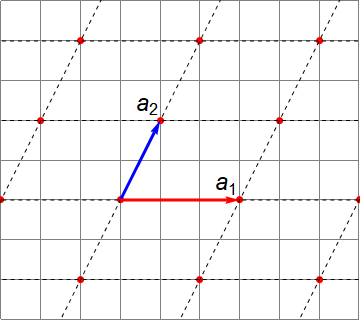
\includegraphics[width=0.40\textwidth]{HLBravaisLattice}
~~~
% (b)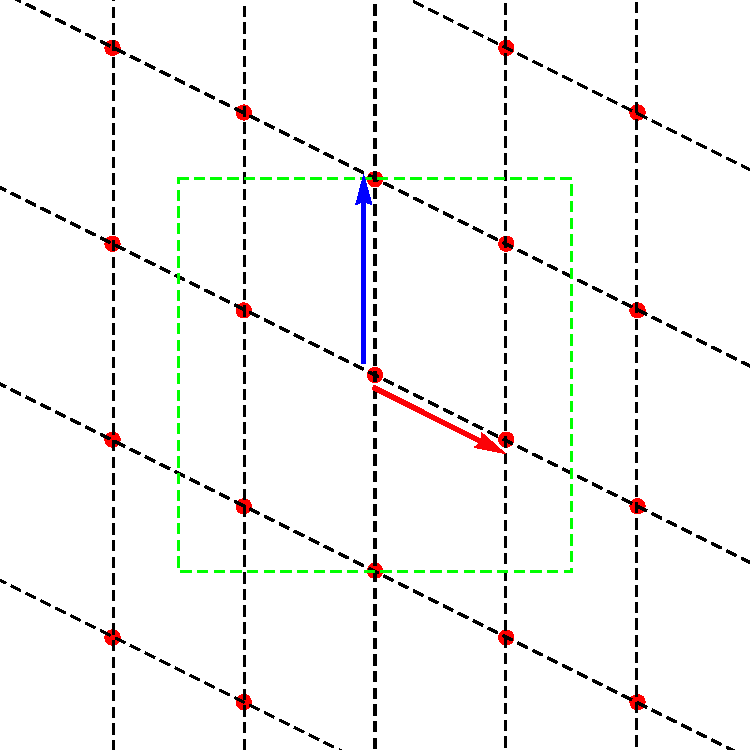
\includegraphics[width=0.40\textwidth]{HLReciprocalLattice1}
  \caption{\label{fig:BravaisLatt}
  (Color online)
%(a)
    The intersections of the (light grey) solid lines form the square
    lattice on which the discrete field $\ssp_z$ is defined. The (red)
    basis vector $\mathbf{a}_1=(3,0)$ and the (blue) basis vector
    $\mathbf{a}_2=(1,2)$ form a $\LTS{}{}{}=\BravCell{3}{2}{1}$ Bravais
    cell. The intersections (red points) of the black dashed lines form
    the Bravais lattice $\lattice$.
% dropped \reffig{fig:HLReciprocalLattice}\'(b)
}
\end{figure}
%%%%%%%%%%%%%%%%%%%%%%%%%%%%%%%%%%%%%%%%%%%%%%%%%%%%%%%%%%%%%%%

A given Bravais \emph{lattice} $\lattice$  can be defined by any of the infinity of
Bravais cells,
each defined by a different pair of basis vectors
$(\mathbf{a}_{1},\mathbf{a}_{2})$, but equivalent under unimodular,
\SLn{2}{\integers} transformation\rf{Lang71}.
    \PC{2020-09-05}{
recheck Lang\rf{Lang71} {\em Linear Algebra}, or replace!
It is possible that it does not reference  modular group at all...
    }
Each such family contains a unique
Bravais cell of the \emph{Hermite normal form}\rf{Cohen93}, which, for a
2\dmn\ square lattice, can be chosen to have the first basis vector
pointing in the spatial direction\rf{Lind96}
\beq
\mathbf{a}_1=\left(\begin{array}{c}
  \speriod{}\\
  0{}
  \end{array}\right)
  \,,\qquad
\mathbf{a}_2=\left(\begin{array}{c}
  \tilt{}\\
  \period{}
  \end{array}\right)
  \,,
\ee{Hermite2d}
where $\speriod{}$, $\period{}$ are respectively the spatial, temporal
lattice periods, and the `tilt'\rf{OKKH99} $0\leq\tilt{}<\speriod{}$ imposes the
relative-periodic `shift' {\bcs}\rf{ChaosBook}
(in the integer lattices literature these are also
referred to as
\emph{`helical'}\rf{LHCLL06} vs. \emph{`toroidal'}\rf{IzOgCh02};
\emph{`twisted'} and
\emph{`twisting factor'}\rf{LHCLL06};
\emph{`screw'}
{\bcs}).
We label Bravais cell \refeq{Hermite2d} and the corresponding Bravais
lattice $\lattice$ by \LTS{}{}{}. An example is the $\BravCell{3}{2}{1}$
Bravais lattice is shown in \reffig{fig:BravaisLatt}.

\PCedit{  %2020-09-05
For each width  $\speriod{}$, height  $\period{}$,
the number of (tilted) Hermite normal form Bravais cells is
\beq
\#_{[\speriod{}\times\period{}]}
   = \sum_{\tilt{}=0}^{\speriod{}-1} 1
   = \speriod{}
\,,
\ee{noBravLatts}
and a Bravais lattices-counting zeta function (see Lind\rf{Lind96}
Example~3.1) can by constructed by substituting
$\#_{[\speriod{}\times\period{}]}$ into
\bea
1/\zeta(z)
 &=& \exp \left(-
 \sum_{\speriod{}=1}^\infty
  \sum_{\period{}=1}^\infty
  \#_{[\speriod{}\times\period{}]}
  \frac{z^{\speriod{}\period{}}}{\speriod{}\period{}}
         \right)
 =  \exp \left(-\sum_{\speriod{}=1}^\infty
                \sum_{\period{}=1}^\infty
    \frac{(z^{\speriod{}})^{\period{}}}{\period{}}
         \right)
\continue
 &=&
   \exp\left(\sum_{\speriod{}=1}^\infty
                \ln(1 - z^{\speriod{}})
         \right)
  =
\prod_{\speriod{}=1}^{\infty}(1 - z^{\speriod{}})
\,.
\label{Lind96Examp3-1}
\eea
    }
    \PC{2020-09-05}{
As long as I do not understand the logic of this zeta function,
we will have to drop it from the paper...
    }


\subsection{Prime Bravais lattices}
\label{s:primeLatt}
% PC{2020-09-05}{ This section was called ``{\em Prime \twots}'' }

It might be possible to tile a given Bravais lattice $\lattice$
by a finer lattice $\lattice_p$. Lattice $\lattice_p$, defined
by a Bravais cell
\beq
\mathbf{a}^p_{1}=\left(\begin{array}{c}
  \speriod{p}\\
  0{}
  \end{array}\right)
  \,,\qquad
\mathbf{a}^p_{2}=\left(\begin{array}{c}
  \tilt{}_{p}\\
  \period{p}
  \end{array}\right)
\,,
\ee{primeTile}
is a \emph{prime} Bravais lattice, if there is no finer Bravais cell,
other than the unit volume $\BravCell{1}{1}{0}$ Bravais cell, that can
tile it.
    \PC{2020-07-15}{
   In \emph{siminos/spatiotemp/chapter/integLatt.tex} Dudgeon and
   Mersereau\rf{DudMer84} explain clearly that if $\det\lattice$ is a
   prime number, then $\lattice$ is a \emph{prime matrix}. If $\lattice$ is
   neither prime nor unimodular, it is \emph{composite}, and can be
   decomposed, nonuniquely - up to a unimodular transformation - into a
   product of two non-unimodular matrices \(\lattice=PQ\). Then one can
   ``quotient'' $Q$ by ``dividing'' by $P$.
    }

In order to determine all prime lattices $\lattice_p$ \refeq{primeTile}
% with Bravais cells \( (\mathbf{a}^p_{1},\mathbf{a}^p_{2}) \,, \)
 that tile a given Bravais lattice $\lattice$ \refeq{Hermite2d},
%with  Bravais cell
%\(
%(\mathbf{a}_1,\mathbf{a}_2)
%\,,
%\)
\bea
\mathbf{a}_1 &=& k\,\mathbf{a}^p_{1} + \ell\,\mathbf{a}^p_{2}
    \continue
\mathbf{a}_2 &=& m\,\mathbf{a}^p_{1} +    n\,\mathbf{a}^p_{2}
\,,
\nnu
\eea
observe that a prime tile
\(
(\mathbf{a}^p_{1},\mathbf{a}^p_{2})
\)
tiles the larger tile only if larger tile's width
$\speriod{}$ is a multiple of $\speriod{p}$, the height
$\period{}$ is a multiple of $\period{p}$, and the two tile `tilts'
satisfy
\[ %beq
\mathbf{a}_2 = {m}\,\mathbf{a}^p_{1} + \frac{\period{}}{\period{p}} \mathbf{a}^p_{2}
\quad\rightarrow\quad
\tilt{} = {m} \speriod{p} + \frac{\period{}}{\period{p}} \tilt{p}
\,.
\] %\ee{primeTiling}
Hence a prime lattice $\lattice_p$ tiles the given lattice $\lattice$ only if
the area spanned by the two `tilted' basis vectors
\beq
\mathbf{a}_2\times\mathbf{a}^p_{2}=\tilt{}\period{p}-\period{}\tilt{p}
\ee{primeTiling}
is a multiple of the prime tile area $\speriod{p}\period{p}$.

    \PCedit{ %2016-11-08
\subsection{Lattice states}
\label{s:lattState}

A \emph{lattice state} is a set of all field values $\Xx = \{\ssp_z\}$
over the $d$\dmn\ lattice $z\in\integers^d$ that satisfies the
\catlatt\ equation \refeq{catLatt}, with all field values constrained to
$0\leq\ssp_z<1$.

While the {\catlatt} equation \refeq{catLatt} is \emph{equivariant} under
the integer lattice \emph{space group} $p4mm$ symmetry operations
\refeq{eq:C4v}, the individual lattice states either have no symmetry at
all (they are, after all, `turbulent'), or are invariant under subgroups
of space group $p4mm$.  In what follows we quotient only the translational
symmetries, and postpone dazzling the captive reader with the full \Dn{4}
point group reduction to a later, more ponderous publication.
}

    \PCedit{ %2020-09-05
Furthermore, inspection of the \templatt\
\reffig{fig:catCycJacob} suggests that there is a \emph{field symmetry}
under inversion though the center of the $0\leq\ssp_z<1$ unit interval.
Indeed, if
$\Mm=\{\Ssym{n\zeit}\}$, composed of symbols from alphabet
\refeq{catLatt2d}, corresponds to a 2\dmn\ lattice state
${\Xx}_{\Mm}=\{\ssp_{n\zeit}\}$, its conjugation symmetry partner
\beq
\bar{\Mm}=\{\bar{\Ssym{}}_{n\zeit}\}
\,,\qquad \bar{\Ssym{}}_{n\zeit} =
2(s-2)-\Ssym{n\zeit}
\,,
\ee{Mconjug}
corresponds to lattice state
${\bar{\Xx}}_{\bar{\Mm}}=\{1-\ssp_{n\zeit}\}$. So, every lattice state
either belongs to a conjugate pair
$\{{\Xx}_{\Mm},\bar{\Xx}_{\bar{\Mm}}\}$, or is self-dual under
conjugation.
%  P 2020-09-05 tests: $2s-4-(2{s}\!-\!1)=-3$; $2s-4-(0)=2s-4 \Rightarrow 1$
}

While the action of {\jacobianOrb} $\jMorb$ \refeq{dDCatsT} maps
fields $\ssp_{n\zeit}$ to values outside the unit interval, such values
that are then returned back to the  unit interval by integer
\Ssym{n\zeit}. This `$\integers^1$ lattice action' at every \spt\ lattice site
is a peculiarity of the coupled Bernoulli and cat map lattice models, not
a condition that a \spt\ discretization of a generic field theory would
satisfy, and should never be confused with a discretization of spacetime
continuum to integer lattice $\integers^d$.



For brevity, we shall refer to lattice state $\Xx$ as a
\emph{\twot} if it satisfies
\beq
\Xx({z} + {R}) = \Xx({z})
\ee{dDprimePO}
for any discrete translation
\(
{R} =n_{1}\mathbf{a}_{1}+n_{2}\mathbf{a}_{2}
\in \lattice
\,,
\)
where $\{n_{1},n_{2}\}$ are any integers, and
$(\mathbf{a}_{1},\mathbf{a}_{2})$ is a pair of $\integers^2$ integer
lattice vectors that define a \emph{Bravais cell}. We shall always refer
to a Bravais sublattice \HLedit{(sublattice of $\integers^2$)} by its unique {Hermite normal form} {Bravais
cell} \refeq{Hermite2d} \HLedit{(basis?)}, and denote it $\lattice=\LTS{}{}{}$,
a 2\dmn\ doubly-periodic
(relative) \emph{\twot}
\beq
\ssp_{n\zeit} = \ssp_{n + \speriod{}, \zeit}
                 = \ssp_{n+\tilt{}, \zeit+ \period{}}
    \,,\qquad
(n,\zeit)\in\integers^2
\ee{Woods12p6}
with periods $(\speriod{},\period{})$ and tilt $\tilt{}$.

A correct  definition of  a {\em prime} {\twot}\rf{DasBuchMirror} is
subtler than for the 1\dmn\ temporal lattice case. If a given {\twot}
over lattice $\lattice$ is not periodic under translations
\({R}\in\lattice_p\) on any sublattice $\lattice_p$ (except for $\lattice$
itself), we shall refer to it here as a \emph{prime {\twot}}, a \po\ of
the smallest periodicity in all spacetime directions.
    \PC{2020-09-08}{
The $\integers^d$ unit cell is always one of $\lattice_p$, see
\reftab{tab:LxTs}, do we say that anywhere?
    }
We return to explicit construction of prime \twots\ in \refsect{s:prime}.
Prime \twots\ are the basic building blocks of \tzeta s (see
\refsect{s:bernZeta} and \ref{s:tempCatZeta}).



Explicitly verifying the periodic lattice states counting formulas for
several 2\dmn\ \catlatt\ examples is now in order.

The simplest examples of {\twots} are
(i) spacetime \eqva\ over $\BravCell{1}{1}{0}$,
(ii) space-\eqva\ over $\BravCell{1}{\period{}}{0}$,
(iii) time-\eqva\  over $\BravCell{\speriod{}}{1}{0}$,
and
(iv) time-\reqva\ over $\BravCell{\speriod{}}{1}{\tilt{}}$,  $\tilt{}\neq0$,
stationary patterns in a time-reference frame\rf{PolTor92} moving with a constant
velocity $\tilt{}/\period{}$.

\subsubsection{Spacetime \eqva\ over $\BravCell{1}{1}{0}$.}
\label{s:catLatt1x1}


\subsubsection{Time-\eqva\ over $\BravCell{\speriod{}}{1}{0}$.}
\label{s:catLattLx1}
Consider the time-\eqv\
\(
\ssp_{n\zeit} = \ssp_{n1}
\)
for all spatial sites $n$, and all times $\zeit$.
To see that this is the 1\dmn\ lattice \templatt\ tiles of period
\speriod\ already counted in \refsect{s:tempCatCount}, note that the 5-term
recurrence relation \refeq{CatMap2d} reduces to the 3-term recurrence
\beq
\ssp_{n+1,1}-2({s}_2-1)\,\ssp_{n1}+\ssp_{n-1,1}
     = -\Ssym{n1}
\,,
\ee{eq:CatLattT=1}
where we have temporarily added index `${}_2$' to the stretching parameter
${s}_2$ to indicate that it refers to the 2\dmn\ \catlatt. Comparing with
the \templatt\ \refeq{catMapNewt},
\(
\ssp_{\zeit+1}  -  {s}_1\, \ssp_{\zeit} + \ssp_{\zeit-1}
    =
-\Ssym{\zeit}
\,,
\)
we see that we have already counted all lattice states on Bravais cells of form
$\BravCell{\speriod{}}{1}{0}$, provided we replace
\(
{s}_1\to2({s}_2-1)
\)
in \refeq{1stChebGenF}. For the values chosen in
our numerical examples,
\( {s}_1=3 \)
and
\( {s}_2=5/2 \,,\)
the two counts happen to be the same and given by \refeq{1stChebGenF}.

However, already the smallest \emph{relative}-periodic
\BravCell{\speriod{}}{1}{\tilt{}}
%$\BravCell{\speriod{}}{1}{0}_\tilt{}$
Bravais lattices are new, and perhaps
surprising.

\subsubsection{Relative  $\BravCell{2}{1}{1}$ \twot.}
\label{s:catLattRel2x1}

% was in siminos/spatiotemp/chapter/CL18blog.tex
% \HLpost{2019-08-08}{
Consider a $\BravCell{2}{1}{1}$ \twot\ with tilt periodic \bcs,
periodic state
\(
\Xx_{\Ssym{1}\Ssym{2}} =
 [
 \begin{array}{cc}
 \ssp_{1} & \ssp_{2}
 \end{array}
 ]
\,,
\)
tiled by the Bravais lattice
\refeq{2DBravaisLattice} with basis vectors $\mathbf{a}_1=\{2,0\}$ and $\mathbf{a}_2=\{1,1\}$, see \reffig{fig:2x1rpo}\,(a).
    \PC{2020-02-23}{
This is wrong, it is written for the symmetric alphabet that we do not use. Fix.
    }	
\beq
\Xx_{\underline{\Ssym{}}\Ssym{}} = \frac{1}{9}
 \left[
 \begin{array}{cc}
 -\Ssym{} & \Ssym{}
 \end{array}
 \right]
        \,,\qquad
\Ssym{}\in\A
         \,,
\ee{catLattRel2x1}
for example
\[
\Mm =
 \left[
 \begin{array}{cc}
 -4 & 4
 \end{array}
 \right]
 \Rightarrow\quad
\Xx_{\underline{4}4} = \frac{1}{9}
 \left[
 \begin{array}{cc}
 -4 & 4
 \end{array}
 \right]
 \,.
\]
Note that these are `periodic lattice state' solutions: there is one \emph{prime}
\twot\ for each set of period-2 periodic lattice states related by cyclic
permutations,
\(
\cycle{\underline{\Ssym{}}\Ssym{}}
    =
(\Xx_{\underline{\Ssym{}}\Ssym{}}, \Xx_{\Ssym{}\underline{\Ssym{}}})
\,,
\)
and there are only 4 of those, as $\Xx_{00}=\Xx_{0}$ is a repeat of the
1-\brick.

By \refeq{2x1_1Fourier} the number of $\BravCell{2}{1}{1}$ relative
\twots\ with the given Bravais lattice bc's is 9.
Using the Green's function method \refeq{GreenFuncCoupled} one can verify
that there are indeed 9 such \twots,
one \twot\ solution for each letter of alphabet \refeq{catLatt2d},

\subsubsection{$\BravCell{2}{1}{0}$ \twot.} %$[2\!\times\!2]$
\label{s:catLatt2cycles}
    %
    %    \HLpost{2019-08-12}{
As an illustration of the {\fundPip} \refeq{detBern0}
counting of periodic solutions, consider \PV\
$s=3$ cat map \refeq{eq:StateSpCatMap} acting on states $\ssp_{\zeit}$
within the unit square $(\ssp_{0},\ssp_{1})\in|0,1)\times|0,1)$. In 2
time steps {\jacobianOrb} $\jMorb$ % $(\jMat^2 - \id)$
stretches the
unit square into the {\fundPip}, with integer points within the
{\fundPip} corresponding to $N_2=5$ periodic lattice states
\refeq{1stChebGenF} of period 2. These integer-valued vertices
over-count the number distinct lattice states, as already noted in the
construction of the \tzeta\ \refeq{Isola90-13a}.

%\paragraph{Symmetries.}

But the great thing about the \catlatt\ is that it is a field theory
defined on a lattice, a theory that can be solved by the well-developed
crystallographic methods: here we follow the
notation of Dresselhaus \etal\rf{Dresselhaus07}.

%    \HLpost{2019-11-22}{
To determine the {\em \admissible} \brick s,

(7)
compute $\Xx_p$ for each prime \brick\ $\Mm_p$, and eliminate every
$\Xx_p$ which contains a lattice site or sites on which the
value of the field violates the admissibility
condition $\ssp_z\in[0,1)$.

For $s=5/2$ \catlatt\
the pruning turns out to be very severe.
Only 52 of the prime
\PCedit{$\BravCell{2}{2}{0}$} % 2019-11-22 Han's was $[4\times4]$
{\brick}s are {\admissible}. As for the repeats of smaller {\brick}s,
there are 2 {\admissible} $\BravCell{1}{2}{0}$ {\brick}s repeating in time and 2
$\BravCell{2}{1}{0}$ {\brick}s repeating in space. There are 4 {\admissible}
$1/2$-shift periodic boundary $\BravCell{1}{2}{0}$ {\brick}s. And there is 1
admissible {\brick} which is a repeat of letter 0.
The total number of $\BravCell{2}{2}{0}$ of \twots\ is obtained by all cyclic
permutations of \admissible\ prime \brick s,
\bea
N_{\BravCell{2}{2}{0}} &=& 225
 \continue
    &=&       {52}\,\BravCell{2}{2}{0}
             + {2}\,\BravCell{2}{1}{0}
             + {2}\,\BravCell{1}{2}{0}
             + {4}\,\BravCell{2}{1}{1}
             + {1}\,\BravCell{1}{1}{0}
\,,
\label{[2x2]count}
\eea
summarized in \reftab{tab:LxTs=5/2}. This explicit list of \admissible\
prime \twots\ verifies the counting formula \refeq{2DCountingFormula}.
%    }

\subsubsection{$\BravCell{3}{2}{0}$ \twot.}
\label{s:catLattRel3x2}
%    \HLpost{2019-11-23}{
For $s=5/2$ \catlatt\
only 850 prime $\BravCell{3}{2}{0}$ \brick s are \admissible. There are 5
\admissible\ repeating prime $\BravCell{3}{1}{0}$ \brick s, 2 \admissible\
repeating prime $\BravCell{1}{2}{0}$ \brick s, and 1 \admissible\ \brick\ which
is a repeat of 0. The total number of \admissible\ solutions obtained by
all cyclic permutations of \admissible\ prime \brick s is:
     \beq
N_{\BravCell{3}{2}{0}} = 5120
=850\,\BravCell{3}{2}{0}+5\,\BravCell{3}{1}{0}+2\,\BravCell{1}{2}{0}+1\,\BravCell{1}{1}{0}
\,,
     \ee{[3x2]count}
summarized in \reftab{tab:LxTs=5/2}.
The count is in agreement with the counting formula \refeq{2DCountingFormula}
for the $\BravCell{3}{2}{0}$ \twots.


\subsubsection{Relative $\BravCell{3}{2}{1}$ \twot.}
\label{s:catLattRel3x2_1}
Consider the Bravais lattice of \reffig{fig:BravaisLatt}, tiled by \twot\
defined by the Bravais cell with basis vectors $\mathbf{a}_1=(3,0)$ and
$\mathbf{a}_2=(1,2)$, see \reffig{fig:2x1rpo}\,(b). There are 6 independent
field values in the repeating cell, which can be written as an
$[3\!\times\!2]$ array:
    \PC{2020-02-23}{
Where is the source code for \reffig{fig:2x1rpo}?
    }
\[
\BravCell{3}{2}{1} =
 \left[
 \begin{array}{cccc}
           & \ssp_{11} & \ssp_{21} & \ssp_{01} \\
 \ssp_{00} & \ssp_{10} & \ssp_{20} &
 \end{array}
 \right]
\,.
\]

\noindent{\em Example: $\BravCell{2}{2}{0}$ Bravais
                lattices prime {\brick}s.}
%\label{s:prime2tori2x2}

%    \HLpost{2019-11-22}{
Consider $\BravCell{2}{2}{0}$ Bravais
lattices prime {\brick}
\beq
\Mm_p=
        \left[\begin{array}{cc}
\Ssym{01} & \Ssym{11}   \\
\Ssym{00} & \Ssym{10}
              \end{array}\right]
\,,
\ee{eq:block2x2}


According to \refeq{primeCount2D}, the number of prime % primitive
$\BravCell{2}{2}{0}$ lattice states is
\bea
M_{\BravCell{2}{2}{0}}&=&\frac{1}{2\cdot2}
  \left( N_{\BravCell{2}{2}{0}}
            - 2M_{\BravCell{2}{1}{0}}
%    \right.\ceq\left.\qquad\qquad
            - 2M_{\BravCell{1}{2}{0}}
            - 2M_{\BravCell{2}{1}{1}}
            - M_{\BravCell{1}{1}{0}}
  \right)
\,,
\label{catlattM2x2}
\eea
We can work this out explicitly as follows:\\

(3) The $\BravCell{2}{1}{1}$ relative-periodic {\brick} \refeq{eq:block2x1rp} is
counted as the $\BravCell{2}{2}{0}$ \twot.

(5) Throw away all {\brick}s which are repeats of
shorter {\brick}s. There are three kinds of repeating small {\brick}s:
\[
\BravCell{2}{1}{0}=\left[\begin{array}{cc}
a & b \\
a & b \\
              \end{array}\right]
\, , \quad
\BravCell{1}{2}{0}=\left[\begin{array}{cc}
b & b \\
a & a \\
              \end{array}\right]
\, , \quad
\BravCell{2}{1}{1}=\left[\begin{array}{ccc}
  & a & b \\
a & b &   \\
              \end{array}\right]
\,.
\]


\bigskip

the relative-periodic $\BravCell{2}{1}{1}$ {\brick} with $1$ site-shift
periodic boundary, which is periodic after the second repeat in the time
direction,
\beq
\Mm_p=
        \left[\begin{array}{ccc}
           &  \left[\Ssym{00}\right.&\left.\Ssym{10}\right] \\
\left[\Ssym{00}\right.&\left.\Ssym{10}\right] &
         \end{array}\right]
\,.
\ee{eq:block2x1rp}


\noindent{\em Example: $\BravCell{3}{2}{0}$  Bravais
                lattices prime {\brick}s.}
%\label{s:prime2tori3x2}

Consider the Bravais lattice
\beq
\Mm=
        \left[\begin{array}{ccc}
\Ssym{12} & \Ssym{22} & \Ssym{32}   \\
\Ssym{11} & \Ssym{21} & \Ssym{31}
              \end{array}\right]
\,.
\ee{eq:block3x2}
According to \refeq{primeCount2D}, the number of prime %primitive
$\BravCell{3}{2}{0}$ lattice states is
\bea
M_{\BravCell{3}{2}{0}}&=&\frac{1}{3\cdot2}
  \left( N_{\BravCell{3}{2}{0}}
            - 3M_{\BravCell{3}{1}{0}}
%    \right.\ceq\left.\qquad\qquad
            - 2M_{\BravCell{1}{2}{0}}
            - M_{\BravCell{1}{1}{0}}
  \right)
\,,
\label{catlattM3x2}
\eea
Unlike the $\BravCell{2}{2}{0}$ case \refeq{eq:block2x1rp}, there no sub-\brick s
with relative-periodic boundary contributing to the $\BravCell{3}{2}{0}$ \brick s
count, since $\BravCell{3}{1}{0}$ and $\BravCell{1}{2}{0}$ sub-\brick s cannot fit into
the $\BravCell{3}{2}{0}$ doubly-periodic Bravais lattice without a shift.

\subsection{Counting \catlatt\ lattice states}
\label{s:catLattCount}

We now show how to count the number of periodic lattice states of a $2$\dmn\
\catlatt, and apply the method
to counting {\twots} of the 2\dmn\ \catlatt.

Periodic lattice {\HillDet}s, such as \refeq{detBern0}, are usually
evaluated by a Fourier transform diagonalization (see
\refappe{appe:Fourier}). However, due to the uniformity of Bernoulli map
stretching, in case at hand lattice points counting is a combinatorial
problem. Counting of $\integers^d$ integer lattice points within various
convex domains is an important, highly developed field. For integer
lattice counting powerful combinatorial methods are available, for
example Barvinok multivariate generating functions algorithm for counting
lattice points in convex lattice domains\rf{Barvinok94}, and its online
code implementations, such as the lattice point enumeration
\texttt{LattE} code\rf{DeLHTY04}.

As in the \templatt\ case \refeq{detCat0}, the total number of periodic
lattice states is given by the volume of the {\fundPip}
\beq
N_\cl{} = |\Det\jMorb|
\,.
\ee{detCatlatt}

\subsection{\Po\ theory}
\label{s:catLattPoThe}

    \PC{2020-02-02}{
Gutkin and Osipov\rf{GutOsi15} refer to an \sPe\ \twot\ solution $p$ as a
`many-particle periodic orbit', with $\ssp_{n\zeit}$ `doubly-periodic',
or `closed,'
\[
\ssp_{n\zeit} = \ssp_{n+\speriod{p},\zeit+\period{p}}
    \,,\quad
n = 0,1,2,\cdots, \speriod{p}-1
    \,;\quad
\zeit = 0,1,2,\cdots, \period{p}-1
    \,.
\]
    }


\subsection{Shadowing}
\label{s:catLattShadow}

    \PC{2019-08-06}{
Must emphasize {\em shadowing}? One of the main points of this and the
companion papers is that \po s shadowing generalizes to \twots\ shadowing
in higher \spt\ dimensions. Include 2d \twots\ shadowing figures.

Add a shadowing sub-section here, the analogue to
\templatt\ Green's function \refeq{1dLatGreenFct}.
    }


As we now show, the
{\brick}
\(
\Mm= \{\Ssym{nt} \in \A \,,\; (n,t)\in \integers^2 \}
\)
can be used as a 2\dmn\ symbolic representation of the lattice system
state.
By the linearity of equation \refeq{2dCoupledCats}, every solution \Xx\
can be uniquely recovered from its symbolic representation \Mm. Inverting
\refeq{2dCoupledCats} we obtain
\beq
  \ssp_{z}=\sum_{z'\in\integers^2}g_{z z'} \Ssym{z'}, \qquad  g_{z z' }
       =\left(\frac{1}{-\Box +2(s -2)}\right)_{zz'}
       \,,
\ee{GreenFuncCoupled}
where  $g_{z z'}$
% $z=(n,t)\in\Zz$,  $z'=(n',t')\in\Zz$,
is the  Green's
function for the 2\dmn\ discretized \sPe.
However, a given lattice \brick\ $\Mm$ %=\{\Ssym{z}|z\in\Zz\}$
is \emph{{\admissible}} if and only if all  $\ssp_{z}\in \Xx$ given by
\refeq{GreenFuncCoupled} fall into the interval $[0,1)$.

For a given
admissible source \brick\ $\Mm$, the periodic field can be computed by:
\[
\Xx_{i_1 j_1} =
\sum_{i_2=0}^2 \sum_{j_2=0}^1 \gd_{i_1 j_1,i_2 j_2} \Mm_{i_2 j_2} \, .
\]
For example, if the source $\Mm$ is:
\[
\Mm =
 \left[
 \begin{array}{ccc}
 0 & 2 & 0 \\
 -1 & 0 & 0
 \end{array}
 \right] \, ,
\]
the corresponding field is:
\[
\Xx_\Mm =
 \left[
 \begin{array}{ccc}
 \ssp_{01} & \ssp_{11} & \ssp_{21} \\
 \ssp_{00} & \ssp_{10} & \ssp_{20}
 \end{array}
 \right]
 =
 \frac{1}{35}
 \left[
 \begin{array}{ccc}
 5 & 17 & 6 \\
 -1 & 5 & 3
 \end{array}
 \right] \, .
\]
Substitute this solution into \reffig{fig:2x1rpo}\,(b) we
can see that \refeq{CatMap2d} is satisfied everywhere.

\subsection{{\Tzeta}}
\label{s:catLattZeta}

\subsection{\catLatt\ as a continuous time dynamical system}
\label{s:catLattODE}

\beq
 (\Box -2(s-2))\,\Xx = -\Mm
\ee{LinearCatLatt}

While the $d=2$ \catlatt\ does have a Hamiltonian
formulation\rf{GutOsi15}, its Lagrangian  formulation as {\sPe}
\refeq{LinearCatLatt}, in analogy with the {\templatt} \refeq{OneCat}, is
a natural departure point for what follows:
\bea
 (\Box -2({s}-2))\,\ssp_{n\zeit} &=& -\Ssym{n\zeit}
    \,, \qquad
  \ssp_{n\zeit} \in [0,1)
    \,, \quad
  \Ssym{n\zeit} \in \A
    \,, \quad
  (n,\zeit)\in \integers^{2}
\,,
\label{2dCoupledCats}
\eea
where $\Box$ is now the discrete 2\dmn\ space-time Laplacian
on $\integers^2$,
\beq
\Box\,\ssp_{n\zeit} =                   \ssp_{n,t-1} + \ssp_{n-1,t}
                   - 4\,\ssp_{n\zeit} + \ssp_{n,t+1} + \ssp_{n+1,t}
\,,
\ee{2dLaplSpaceTime}
and the alphabet is given in \refeq{catLatt2d}.

    \PC{2019-01-04} {
More generally, the same argument yields the {\sPe} \refeq{OneCat} for
the $d$\dmn\ {\em \catlatt}
\bea
 (\Box - d({s}-2))\,\ssp_{z} &=& -\Ssym{z}
    \,, \qquad
  \ssp_{z} \in [0,1)
    \,, \quad
  \Ssym{z} \in \A
    \,, \quad
  z\in \integers^{d}
\,,
\continue
 && \A = \{-2d+1, -2d+2,\cdots,2{s}-2,2{s}-1\}
\,,
\label{LinearConn}
\eea
where $\Box$ is the discrete $d$\dmn\ Euclidean space-time Laplacian.
}

    \PC{2019-01-04} {

The $d$\dmn\ \catlatt\ satisfies {\sPe} \refeq{dDCatsT}
\beq
(\Box -d(s - 2))\,\ssp_{z} =-\Ssym{z}
\,,\qquad
{z} \in \integers^d
\,,
\ee{dDCats}
where $\Box$ is the discrete $d$\dmn\ Laplacian
(discrete Laplacians on 1\dmn\ and 2\dmn\ lattices are given in
\refeq{PerViv2.2} and \refeq{2dLaplSpaceTime}). As in \refeq{action}, a
$d$\dmn\ discrete Laplacian can be written as
\beq
\Box = \sum_{i=1}^{d} (\hopMat_{i}  - 2\id + \hopMat_{i}^{-1})
\,,
\ee{dDLapl}
    }


------------------------------------------------------

\bigskip

\noindent\textbf{\catLatt, summarized.}
The
key insight\rf{BunSin88,GutOsi15} --an insight that applies to coupled-map
lattices\rf{PolTor92b,PetCorBol06,PetCorBol07}, and field theories
modeled by them, not only the system considered here-- is that a field
\(
\Xx=\{\ssp_{z}\} % = \{\ssp_{z},  z\in \integers^{d}  \}
\)
over a $d$\dmn\ spacetime lattice $z\in \integers^{d}$ has to be
described by a corresponding symbol {\brick}
\(
\Mm=\{\m_{z}\} % = \{\m_{z}, z\in \integers^{d}\}
\,,
\)
over the same $d$\dmn\ spacetime  lattice $z\in \integers^{d}$, rather
than a 1\dmn\ temporal symbol sequence \refeq{linCode}, as one does when
describing a finite coupled ``$N$-particle'' system in the Hamiltonian
formalism.

A key advantage of the {\spt} code \Mm\ is illustrated already by the $d=2$
case. While an \AW\ type partition, forward-in time Hamiltonian evolution
alphabet would grow exponentially with the
``particle number'' $\speriod{}$, the number of letters
\refeq{dDCatsT} of the {\spt} code \A\ is finite and the same for any
spatial extent
$\speriod{}$, including the $\speriod{}\to\infty$ \catlatt. For the
{\spt} code, a field \Xx\ over a periodic \spt\ domain is encoded by a
doubly periodic 2\dmn\ {\brick} $\Mm$ of symbols from a small alphabet,
rather then by a $1$\dmn\ temporal string of symbols from the
exponentially large (in $\speriod{}$) `\speriod{}-particle' alphabet
\Aa.

The
{\catlatt} is arguably the simplest example of a chaotic (or `turbulent')
classical field theory for which the local degrees of freedom are
hyperbolic (anti-harmonic, `inverted pendula') rather than oscillatory
(`harmonic oscillators'). As we have shown here, it is also a field theory
for which all {\admissible} {\spt} patterns can be enumerated, and their
recurrences (shadowing of a large \twot\ by smaller \twots) identified.

    \ifboyscout\clearpage\fi
% siminos/spatiotemp/chapter/prime.tex  % called by blogCats.tex and CL18.tex
% $Author: predrag $ $Date: 2021-08-10 11:56:19 -0400 (Tue, 10 Aug 2021) $

\section{Enumeration of prime \twots}
\label{sect:Count2dprimePO}

\begin{description}

    \PCpost{2020-08-10}{
Copied to  \emph{siminos/kittens/prime.tex}, in  \emph{CL18.tex}
The two versions are from now on edited separately
	}

\end{description}


\subsection{Covering alphabet}
\label{sect:prime2tCover}

Our algorithm for generating all prime $\LTS{}{}{}$ Bravais
lattices consists in picking the lexically lowest \brick\
for every set of \brick s related by spatial and temporal translations:
\begin{enumerate}
  \item
Fill the first row
\(
\left[\Ssym{11}\;\Ssym{21}\cdots\Ssym{\speriod{}1}\right]
\)
by lexically ordered symbols,
\(
\Ssym{j1}\leq\Ssym{j+1,1}\,,
\)
keep one \brick\ for each set of spatially cyclically related
permutations.
  \item
Picking the lexically ordered first row representatives uses up the
cyclic invariance under spatial translations, so for the second
\(
\left[\Ssym{12}\;\Ssym{22}\cdots\Ssym{\speriod{}2}\right]
\)
and higher rows fill in all $|\A|^\period{}$ combinations of  symbols.
  \item
The count is the same for all $\LTS{}{}{}$
relative-periodic {\brick}s.
  \item
Group \brick s into sets related by cyclic permutations in the time
direction. For each such set, pick a representative that has lexically
lowest first row, throw away the rest.
  \item
Throw away all {\brick}s which are repeats of
shorter {\brick}s in the spatial direction.
  \item
Throw away all {\brick}s which are repeats of
shorter {\brick}s in the temporal direction. What
remains in $N_k$ prime periodic \brick s $p$ of the same size
$[\speriod{p}\times\period{p}]=[\speriod{k}\times\period{k}]$.
  \item
The total number
of (doubly) periodic
\brick s is the sum of all cyclic permutations of prime \brick s,
\[
|\A|^{\speriod{}\period{}}
=
\sum_p N_{p}\,\LTS{p}{p}{p}
\]
where the sum goes over prime tilings of the $\LTS{}{}{}$
\brick.
\end{enumerate}
This completes the list of prime \twots, with the alphabet $\A$ taken
as a {\em covering} alphabet, \ie, we have generated all possible prime
\brick s, under assumption of no grammar rules.

\PCedit{
The number of prime \twots\ is given recursively by
(see \refeq{primeCount}),
\beq
M_{p}\,=\,\frac{1}{\speriod{}\period{}}
  \left( N_{p}
          - \sum _{p'}
            \speriod{p'}\period{p'}
                                          \, M_{p'}
  \right)
\,,
\ee{primeCount2D}
where the sum is over $p'$, the prime `divisors' of $p$
that satisfy tiling conditions \refeq{primeTiling}.
    }

\bigskip

\noindent{\em Example: $\BravCell{2}{2}{0}$ Bravais
                lattices prime {\brick}s.}
%\label{sect:prime2tori2x2}

%    \HLpost{2019-11-22}{
Consider $\BravCell{2}{2}{0}$ Bravais
lattices prime {\brick}
\beq
\Mm_p=
        \left[\begin{array}{cc}
\Ssym{01} & \Ssym{11}   \\
\Ssym{00} & \Ssym{10}
              \end{array}\right]
\,,
\ee{eq:block2x2}
and the relative-periodic $\BravCell{2}{1}{1}$ {\brick} with $1$ site-shift
periodic boundary, which is periodic after the second repeat in the time
direction,
\beq
\Mm_p=
        \left[\begin{array}{ccc}
           &  \left[\Ssym{00}\right.&\left.\Ssym{10}\right] \\
\left[\Ssym{00}\right.&\left.\Ssym{10}\right] &
         \end{array}\right]
\,.
\ee{eq:block2x1rp}
According to \refeq{primeCount2D}, the number of prime % primitive
$\BravCell{2}{2}{0}$ {\lattstate}s is
\bea
M_{\BravCell{2}{2}{0}}&=&\frac{1}{2\cdot2}
  \left( N_{\BravCell{2}{2}{0}}
            - 2M_{\BravCell{2}{1}{0}}
%    \right.\ceq\left.\qquad\qquad
            - 2M_{\BravCell{1}{2}{0}}
            - 2M_{\BravCell{2}{1}{1}}
            - M_{\BravCell{1}{1}{0}}
  \right)
\,,
\label{catlattM2x2}
\eea
We can work this out explicitly as follows:\\
(1)
Fill the first row
\(
\left[\Ssym{11}\;\Ssym{21}\right]
\)
by lexically ordered symbols, one for each set of spatially cyclically related
permutations. For the alphabet \refeq{catLatt2d} there
are 36
such length 2 strings.

(2) As we have already `used up' the cyclic invariance under spatial
translations by picking the lexically ordered first row representatives,
for the second
\(
\left[\Ssym{12}\;\Ssym{22}\right]
\)
and higher rows all 81 combinations of 9 symbols are allowed.
We now have $36\times81 =2916$ {\brick}s in all.

(3) The $\BravCell{2}{1}{1}$ relative-periodic {\brick} \refeq{eq:block2x1rp} is
counted as the $\BravCell{2}{2}{0}$ \twot; as in (1), after spatial cyclic
rotations, there are 36 such prime {\brick}s.

(4) Group \brick s into sets related by cyclic permutations in the time
direction. For each such set, pick a representative that is lexically
lowest in the first row, throw away the rest.

(5) Throw away all {\brick}s which are repeats of
shorter {\brick}s. There are three kinds of repeating small {\brick}s:
\[
\BravCell{2}{1}{0}=\left[\begin{array}{cc}
a & b \\
a & b \\
              \end{array}\right]
\, , \quad
\BravCell{1}{2}{0}=\left[\begin{array}{cc}
b & b \\
a & a \\
              \end{array}\right]
\, , \quad
\BravCell{2}{1}{1}=\left[\begin{array}{ccc}
  & a & b \\
a & b &   \\
              \end{array}\right]
\,.
\]
(6)
The result is 1584 $\BravCell{2}{2}{0}$ prime {\brick}s.

There are also 36 prime $\BravCell{2}{1}{0}$ {\brick}s repeating in time, 36
prime $\BravCell{1}{2}{0}$ {\brick}s repeating in space, 36 prime $\BravCell{2}{1}{1}$
{\brick}s repeating in time with $1/2$-shift periodic boundary, and 9
{\brick}s which are repeats of one-symbol prime $\BravCell{1}{1}{0}$ {\brick}.
The total number
of \PCedit{$\BravCell{2}{2}{0}$} % 2019-11-22 Han's was $[4\times4]$
\brick s is recovered by all cyclic permutations of prime \brick s \refeq{catlattM2x2}:
\bea
N_{\BravCell{2}{2}{0}} &=& 9^{2\times2} = 6561
    \label{catlattN2x2}\\
    &=&        {1584}\,\BravCell{2}{2}{0}
             + {36}\,\BravCell{2}{1}{0}
             + {36}\,\BravCell{1}{2}{0}
             + {36}\,\BravCell{2}{1}{1}
             + {9}\,\BravCell{1}{1}{0}
\,,
\nnu
\eea
where $\cycle{\cdots}$ stands for the number of prime {\brick}s
of a given shape.
This completes the count with the alphabet
\refeq{catLatt2d} taken as a {\em covering} alphabet, \ie, we
have generated all possible prime \brick s, were there no further grammar
rules.

\bigskip

\noindent{\em Example: $\BravCell{3}{2}{0}$  Bravais
                lattices prime {\brick}s.}
%\label{sect:prime2tori3x2}

Consider the Bravais lattice
\beq
\Mm=
        \left[\begin{array}{ccc}
\Ssym{12} & \Ssym{22} & \Ssym{32}   \\
\Ssym{11} & \Ssym{21} & \Ssym{31}
              \end{array}\right]
\,.
\ee{eq:block3x2}
According to \refeq{primeCount2D}, the number of prime %primitive
$\BravCell{3}{2}{0}$ {\lattstate}s is
\bea
M_{\BravCell{3}{2}{0}}&=&\frac{1}{3\cdot2}
  \left( N_{\BravCell{3}{2}{0}}
            - 3M_{\BravCell{3}{1}{0}}
%    \right.\ceq\left.\qquad\qquad
            - 2M_{\BravCell{1}{2}{0}}
            - M_{\BravCell{1}{1}{0}}
  \right)
\,,
\label{catlattM3x2}
\eea
Unlike the $\BravCell{2}{2}{0}$ case \refeq{eq:block2x1rp}, there no sub-\brick s
with relative-periodic boundary contributing to the $\BravCell{3}{2}{0}$ \brick s
count, since $\BravCell{3}{1}{0}$ and $\BravCell{1}{2}{0}$ sub-\brick s cannot fit into
the $\BravCell{3}{2}{0}$ doubly-periodic Bravais lattice without a shift.

Following the same algorithm as for $\BravCell{2}{2}{0}$ \brick s, we get 88440
$\BravCell{3}{2}{0}$ prime \brick s, 240 prime $\BravCell{3}{1}{0}$ \brick
s repeating in time, 36 prime $\BravCell{1}{2}{0}$ \brick s repeating in space,
and 9 \brick s which are repeats of one symbol prime $\BravCell{1}{1}{0}$ \brick.
The total number of $\BravCell{3}{2}{0}$ \brick s is recovered by all cyclic
permutations of prime \brick s:
\bea
N_{\BravCell{3}{2}{0}} &=& 9^{3\times2} = 531441
    \continue
 &=& 88440\,\BravCell{3}{2}{0}+240\,\BravCell{3}{1}{0}
       +36\,\BravCell{1}{2}{0}+9\,\BravCell{1}{1}{0}
\,.
\label{catlattN3x2}
\eea



\subsection{Admissible prime \twots}
\label{sect:prime2tAdmiss}

To determine the {\em \admissible} \brick s, compute $\Xx_p$ for each
prime \brick\ $\Mm_p$, and eliminate every $\Xx_p$ which contains a
lattice site or sites on which the value of the field violates the
admissibility condition $\ssp_z\in[0,1)^2$.

%%%%%%%%%%%%%%%%%%%%%%%%%%%%%%%%%%%%%%%%%%%%%%%%%%%%%%
\ifblog
% siminos/spatiotemp/tables/LxTs5o2.tex
% $Author: predrag $ $Date: 2021-08-10 11:56:19 -0400 (Tue, 10 Aug 2021) $

%%%%%%%%%%%%%%%%%%%%%%%%%%%%%%%%%%%%%%%%%%%%%%%%%%%%%%
% called by blogCats.tex and CL18.tex
% 2020-06-09 HL siminos/mathematica/PrimeSolutions.nb
%            Edited the tables of numbers of prime solutions
% Predrag 2019-11-23 started with ChaosBook \reftab{tab:primeTwots}
\begin{table}
\caption[]{\label{tab:LxTs=5/2}    \small
The numbers of the ${s}=5/2$ \catlatt\
$\LTS{}{}{}$ \twots: $M_{\LTS{}{}{}}$ is the
number of prime \twots, $N_{\LTS{}{}{}}$ is the
number of doubly periodic {\lattstate}s,
and $R_{\LTS{}{}{}}$ is the number of prime \twots\ in the
$\Dn{4}$ symmetries orbit.
}
\begin{center}
%\renewcommand{\arraystretch}{0.8}
{\small
\begin{tabular}{lrlr}
\\[-16pt]
$\LTS{}{}{}$
                  & $M$ %_{[\speriod{}\!\times\!\period{}]}$
                         & $N$ %_{[\speriod{}\!\times\!\period{}]}$
                                                 &$R$\\
\hline
$\BravCell{1}{1}{0}$  &   1  &   1                   & 1 \\
$\BravCell{2}{1}{0}$  &   2  &
  $5~=\;\;\,2\,\BravCell{2}{1}{0}+1\,\BravCell{1}{1}{0}$
                                                 & 2 \\
$\BravCell{2}{1}{1}$&   4  & 9~\;=\;\;\,$
                           {4}\,\BravCell{2}{1}{1}
                         + {1}\,\BravCell{1}{1}{0}$
                                                 &   \\
$\BravCell{3}{1}{0}$  &   5  & 16 =~ ${5}\,\BravCell{3}{1}{0}
                         + {1}\,\BravCell{1}{1}{0}$
                                                 &   \\
$\BravCell{3}{1}{1}$&   16 & $49 =16\,\BravCell{3}{1}{1}
                         + {1}\,\BravCell{1}{1}{0}$
                                                 &   \\
%$\BravCell{3}{1}{2}$&   16 & $49 =16\,\BravCell{3}{1}{2}  % (49-1)/3
%                         + {1}\,\BravCell{1}{1}{0}$
%                                                 &   \\
$\BravCell{4}{1}{0}$  &  10 & $45 =10\,\BravCell{4}{1}{0} % (45-2*2-1)/4
                         + {2}\,\BravCell{2}{1}{0}
                         + {1}\,\BravCell{1}{1}{0}$
                                                 &   \\
$\BravCell{4}{1}{1}$&   54 & $225 =54\,\BravCell{4}{1}{1} % (225-4*2-1)/4
			+{4}\,\BravCell{2}{1}{1}
                         + {1}\,\BravCell{1}{1}{0}$
                                                 &   \\
$\BravCell{4}{1}{2}$&   60 & $245 =59\,\BravCell{4}{1}{2} % (245-2*2-1)/4
                         + {2}\,\BravCell{2}{1}{0}
                         + {1}\,\BravCell{1}{1}{0}$
                                                 &   \\
%$\BravCell{4}{1}{3}$&   56 & $225 =56\,\BravCell{4}{1}{2}
%                         + {1}\,\BravCell{1}{1}{0}$
%                                                 &   \\
$\BravCell{2}{2}{0}$  &   52  & $225 =
               {52}\,\BravCell{2}{2}{0}
             + {2}\,\BravCell{2}{1}{0}
             + {2}\,\BravCell{1}{2}{0}$
                                                 &   \\
                      &       & $\quad\quad\;\;
             + {4}\,\BravCell{2}{1}{1}
             + {1}\,\BravCell{1}{1}{0}$
                                                 & 1 \\
$\BravCell{2}{2}{1}$&  60 & $245 = 60\,\BravCell{2}{2}{1}  % (245-2*2-1)/4
			+ {2}\,\BravCell{1}{2}{0}
                         + {1}\,\BravCell{1}{1}{0}$
                                                 &   \\
$\BravCell{3}{2}{0}$  & 850  &
                          $ 5\,120 =850\,\BravCell{3}{2}{0}
                          +5\,\BravCell{3}{1}{0}$
                                                 &   \\
                      &       & $\qquad\quad\;\,
                          +2\,\BravCell{1}{2}{0}
                          +1\,\BravCell{1}{1}{0}$
                                                 &   \\
$\BravCell{3}{2}{1}$& 1\,012 &
                           $ 6\,125 =1\,012\,\BravCell{3}{2}{1} %(6125 - 16*3-2*2 -1)/6
                           +16\,\BravCell{3}{1}{2}$
                                                 &   \\
                      &       & $\qquad\quad~~
                           +2\,\BravCell{1}{2}{0}
                           +~\,1\,\BravCell{1}{1}{0}$
                                                 &   \\
%$\BravCell{3}{2}{2}$&      & 6125 =?$\BravCell{3}{2}{2}
%                         + {1}\,\BravCell{1}{1}{0}$
%                                                 &   \\
$\BravCell{3}{3}{0}$  & 68\,281 &

                         $ 614\,656 = 68\,281\,\BravCell{3}{3}{0}
                         +  5\,\BravCell{3}{1}{0}$  %(614656 -2*16*3 - 5*3 - 5*3 -1)/9$
                                                 &   \\
                      &       & $\,
                         + 16\,\BravCell{3}{1}{1} +16 \,\BravCell{3}{1}{2}
                         +  5\,\BravCell{1}{3}{0}
                         + {1}\,\BravCell{1}{1}{0}$
                                                 & 1  \\
$\BravCell{3}{3}{1}$& 70\,400  &
                         $ 633\,616 =70\,400\,\BravCell{3}{3}{1}
                         + {5}\,\BravCell{1}{3}{0} %(633616 - 5*3 -1)/9
                         + {1}\,\BravCell{1}{1}{0}$
                                                 &   \\
%$\BravCell{3}{3}{2}$&      & 633616 =?$\BravCell{3}{3}{2}
%                         + {1}\,\BravCell{1}{1}{0}$
%                                                 &   \\
\end{tabular}
} %end \small
\end{center}
\end{table}
%%%%%%%%%%%%%%%%%%%%%%%%%%%%%%%%%%%%%%%%%%%%%%%%%%%%%%%%%%%%%%%%%%%%%%

\fi
%%%%%%%%%%%%%%%%%%%%%%%%%%%%%%%%%%%%%%%%%%%%%%%%%%%%%%


\begin{description}

    \HLpost{2019-11-22}{
For $s=5/2$ \catlatt\ the pruning is very severe. Of {1584}
covering alphabet prime {\brick}s in \refeq{catlattN2x2}, only 52 prime
\PCedit{$\BravCell{2}{2}{0}$} % 2019-11-22 Han's was $[4\times4]$
{\brick}s are {\admissible}. As for the repeats of smaller {\brick}s,
there are 2 {\admissible} $\BravCell{1}{2}{0}$ {\brick}s repeating in time and 2
$\BravCell{2}{1}{0}$ {\brick}s repeating in space. There are 4 {\admissible}
$1/2$-shift periodic boundary $\BravCell{1}{2}{0}$ {\brick}s. And there is 1
admissible {\brick} $\BravCell{1}{1}{0}$ which is a repeat of letter 0.
The total number of $\BravCell{2}{2}{0}$ of \twots\ is obtained by all cyclic
permutations of \admissible\ prime \brick s (a significant pruning,
compared to the full shift count \refeq{catlattN2x2}),
\bea
N_{\BravCell{2}{2}{0}} &=& 225
 \label{HL[2x2]count}\\
    &=&       {52}\,\BravCell{2}{2}{0}
             + {2}\,\BravCell{2}{1}{0}
             + {2}\,\BravCell{1}{2}{0}
             + {4}\,\BravCell{2}{1}{1}
             + {1}\,\BravCell{1}{1}{0}
\,.
\nnu
\eea
    }

    \HLpost{2019-11-23}{
For $s=5/2$ \catlatt\
only 850 prime $\BravCell{3}{2}{0}$ \brick s are \admissible. There are 5
\admissible\ repeating prime $\BravCell{3}{1}{0}$ \brick s, 2 \admissible\
repeating prime $\BravCell{1}{2}{0}$ \brick s, and 1 \admissible\ \brick\ which
is a repeat of 0. The total number of \admissible\ solutions obtained by
all cyclic permutations of \admissible\ prime \brick s is:
     \beq
N_{\BravCell{3}{2}{0}} = 5120
=850\,\BravCell{3}{2}{0}+5\,\BravCell{3}{1}{0}+2\,\BravCell{1}{2}{0}+1\,\BravCell{1}{1}{0}
\,,
     \ee{HL[3x2]count}
in agreement with the counting formula \refeq{2DCountingFormula}
for the $\BravCell{3}{2}{0}$ \twots.
    }

%%%%%%%%%%%%%%%%%%%%%%%%%%%%%%%%%%%%%%%%%%%%%%%%%%%%%%
\ifblog
% siminos/spatiotemp/tables/LxTs.tex
% $Author: predrag $ $Date: 2021-08-10 11:56:19 -0400 (Tue, 10 Aug 2021) $

%%%%%%%%%%%%%%%%%%%%%%%%%%%%%%%%%%%%%%%%%%%%%%%%%%%%%%
% 2020-06-09 HL siminos/mathematica/PrimeSolutions.nb
%            Edited the tables of numbers of prime solutions
% Predrag 2020-02-23    called by blogCats.tex and CL18.tex
\begin{table}
\caption[]{\label{tab:LxTs}     \small
The numbers of \catlatt\ {\lattstate}s for Bravais lattices
$\Lambda=\LTS{}{}{}$ up to $\BravCell{3}{3}{2}$. Here
$N_\Lambda(s)$ is the number of doubly periodic
{\lattstate}s,
$M_\Lambda(s)$ is the number of prime \twots,
and $R_{\Lambda}$ is the number
of prime \twots\ in the $\Dn{4}$ symmetries orbit.
The stretching parameter ${s}$ can take half-integer or integer
values.
}
\begin{center}
%\renewcommand{\arraystretch}{0.8}
{\small
\begin{tabular}{lllr}
\\[-16pt]
$~~~\Lambda$
                         & ~~~$N_\Lambda(s)$ & $M_\Lambda(s)$
                                                 &$R$  \\
\hline
$\BravCell{1}{1}{0}$    &   $2({s}-2)$ & $2({s}-2)$ & 1 \\
$\BravCell{2}{1}{0}$    &   $2({s}-2)2s$ & $2({s}-2)\frac{1}{2}(2{s}-1)$   & 2 \\
$\BravCell{2}{1}{1}$  &   $2({s}-2)2({s}+2)$ & $2({s}-2)\frac{1}{2}(2{s}+3)$  & \\
$\BravCell{3}{1}{0}$    &   $2({s}-2)(2{s}-1)^2$ & $2({s}-2)\frac{4}{3}({s}-1){s}$ &  \\
$\BravCell{3}{1}{1}$  &   $2({s}-2)4({s}+1)^2$ & $2({s}-2)\frac{1}{3}(2{s}+1)(2{s}+3)$ & \\
%was $2({s}-2)(2{s}-1)^2$
%$\BravCell{3}{1}{2}$  &   $2({s}-2)4({s}+1)^2$ & $2({s}-2)\frac{1}{3}(2{s}+1)(2{s}+3)$ & \\
%was $2({s}-2)(2{s}-1)^2$
$\BravCell{4}{1}{0}$    &   $2({s}-2)8({s}-1)^2{s}$ & $2({s}-2)\frac{1}{2}(2{s}-3)(2{s}-1)s$ & \\
$\BravCell{4}{1}{1}$  &   $2({s}-2)8s^2({s}+2)$ & $2({s}-2)\frac{1}{2}({s}+2)(2{s}-1)(2{s}+1)$ & \\
%was $2({s}-2)8({s}-1)^2{s}$
$\BravCell{4}{1}{2}$  &   $2({s}-2)8({s}+1)^2{s}$ & $2({s}-2)\frac{1}{2}(2{s}+3)(2{s}+1)s$     & \\
%was $2({s}-2)8({s}-1)^2{s}$
$\BravCell{4}{1}{3}$  &   $2({s}-2)8s^2({s}+2)$ & $2({s}-2)\frac{1}{2}({s}+2)(2{s}-1)(2{s}+1)$ &  \\
%was $2({s}-2)8({s}-1)^2{s}$
$\BravCell{5}{1}{0}$    & $2({s}-2)\left(4{s}^2-6{s}+1\right)^2$ & $2({s}-2)\frac{4}{5}({s}-1)(2{s}-3)(2{s}-1)s$
                                  & \\
$\BravCell{5}{1}{1}$  & $2({s}-2)16\left({s}^2+{s}-1\right)^2$ & $2({s}-2)\frac{1}{5}(2{s}-1)(2{s}+3)(4{s}^2+4{s}-5)$
                                  & \\
%was $2({s}-2)\left(4{s}^2-6{s}+1\right)^2$
$\BravCell{2}{2}{0}$    & $2({s}-2)8s^2({s}+2)$ & $2({s}-2)\frac{1}{2}(2{s}-1)(2{s}^2+5{s}+1)$  & 1 \\
$\BravCell{2}{2}{1}$  & $2(s-2)8s (s+1)^2$ & $2({s}-2)\frac{1}{2}(2{s}+1)(2{s}+3)s$ &  \\
%was $2(s-2)8s^2 (s+2)$
$\BravCell{3}{2}{0}$    & $2({s}-2)2s(2{s}-1)^2 (2{s}+3)^2$
	& $2({s}-2)\frac{2}{3}(2{s}-1)(4{s}^3+10{s}^2+3{s}-5)s$
                                  &  \\
$\BravCell{3}{2}{1}$  & $2({s}-2)32{s}^3({s}+1)^2$
	& $2 ({s}-2) \frac{1}{6} (2 {s}-1) (2 {s}+1) (8 {s}^3+16 {s}^2+10 {s}+3)$
                                  &  \\
%$\BravCell{3}{2}{2}$  & $2({s}-2)32{s}^3 ({s}+1)^2$
%	& $2 ({s}-2) \frac{1}{6} (2 {s}-1) (2 {s}+1) (8 {s}^3+16 {s}^2+10 {s}+3)$
%                                  &  \\
$\BravCell{3}{3}{0}$    & $2({s}-2)16({s}+1)^4(2{s}-1)^4$
                                  &  \\
$\BravCell{3}{3}{1}$  & $2({s}-2)(2{s}-1)^2(8{s}^3+12{s}^2-1)^2$
	            &  \\
%$\BravCell{3}{3}{2}$  & $2({s}-2)(2{s}-1)^2(8{s}^3+12{s}^2-1)^2$
%                &
\end{tabular}
} %end \small
\end{center}
\end{table}
%%%%%%%%%%%%%%%%%%%%%%%%%%%%%%%%%%%%%%%%%%%%%%%%%%%%%%%%%%%%%%%%%%%%%%

\fi
%%%%%%%%%%%%%%%%%%%%%%%%%%%%%%%%%%%%%%%%%%%%%%%%%%%%%%%%%%%%%%%%%%%%%%

    \HLpost{2020-06-09}{
The \admissible\ prime \twots\ counts for any half-integer or integer
${s}$ are listed in \reftab{tab:LxTs}.
Note that $N_{\BravCell{3}{\period{}}{1}}({s})=N_{\BravCell{3}{\period{}}{2}}({s})$,
by reflection symmetry, as
$N_{\BravCell{3}{\period{}}{2}}({s})=N_{\BravCell{3}{\period{}}{-1}}({s})$.


These two expressions do not
fit into the table format:
\bea
M_{\BravCell{3}{3}{0}}
&=&
2({s}-2)\frac{1}{9}(256 {s}^8+512 {s}^7-128 {s}^6-640 {s}^5
\ceq
\qquad\quad +16 {s}^4+320 {s}^3-48 {s}^2-72 {s}+9)
\,.
\label{HL[3x3]0cnt}
\eea
The last, currently unreduced formula exemplifies what is nonintuitive
about the Fourier space results; it is not at all obvious that this
\bea
M_{\BravCell{3}{3}{1}}
&=&
M_{\BravCell{3}{3}{2}}
=
2 (s-2) \frac{1}{9} (1-2 s)^2 \times
\ceq
\left\{\left[2 s+1-2 \sin \left(\frac{\pi}{18}\right)\right]^2
\left[2 s+1+2 \cos \left(\frac{\pi}{9}\right)\right]^2
     \right.
\ceq
     \left.
~~\left[(2 s+1-2 \cos \left(\frac{2\pi}{9}\right)\right]^2-1
     \right\}
\label{HL[3x3]0count}
\eea
is an
integer for any half-integer or integer ${s}$.
{\bf Predrag} to Han: can you evaluate this using the fundamental fact
$N_\cl{} = |\Det\jMorb|$?
    }

    \HLpost{2020-06-09}{
The \admissible\ prime \twots\ counts are listed in
\reftab{tab:LxTs=5/2}. This list verifies the counting formula
\refeq{2DCountingFormula}.
    }

    \HLpost{2019-11-24}{
The interior alphabet depends on the value of $s$ and the \admissible\
range of $\ssp_z$.
For $s=5/2$, $\ssp_z\in[0,1)$, the interior alphabet is
$\Ai=\{0,1\}$ (see eq.~(38) in \refref{GHJSC16}).
For $s=7/2$, $\ssp_z\in[0,1)$, the interior alphabet is
$\Ai=\{0,1,2,3\}$ (eq.~(46) in \refref{GHJSC16}).
    }

	\HLpost{2020-06-09}{
\refFigs{fig:SpecialBravaisLatt}{fig:3x2rpo} are the plots of the
periodic \brick s by color. The three figures in
\reffig{fig:SpecialBravaisLatt} are the \brick s with periodicity
$\BravCell{1}{3}{0}$, $\BravCell{3}{1}{0}$ and $\BravCell{3}{1}{1}$,
which can show the periodicity of the space-\eqva, time-\eqva\ and
time-\reqva. \refFig{fig:3x2rpo} is the color coding of the periodic
blocks with periodicity $\BravCell{2}{1}{1}$, $\BravCell{3}{2}{1}$ and
$\BravCell{3}{2}{0}$.
	}

%%%%%%%%%%%%%%%%%%%%%%%%%%%%%%%%%%%%%%%%%%%%%%%%%%%%%%%%%%%%%
% HL 2020-06-09 siminos/figSrc/han/Mathematica/ColorBlock.nb
\begin{figure}\begin{center}
            \begin{minipage}[c]{0.25\textwidth}\begin{center}
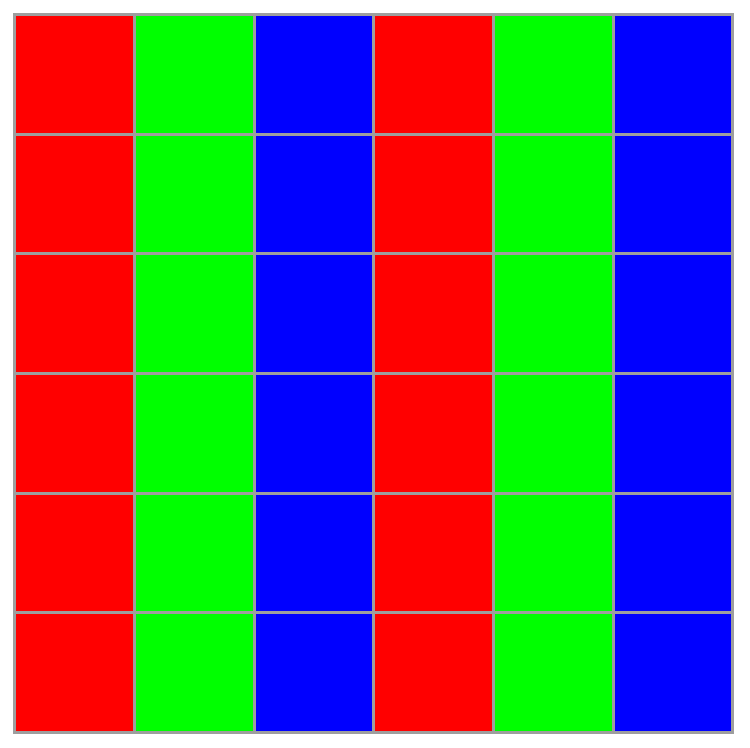
\includegraphics[width=1.0\textwidth]{HL310Block}\\(a)
            \end{center}\end{minipage}
            \hskip 4ex
            \begin{minipage}[c]{0.25\textwidth}\begin{center}
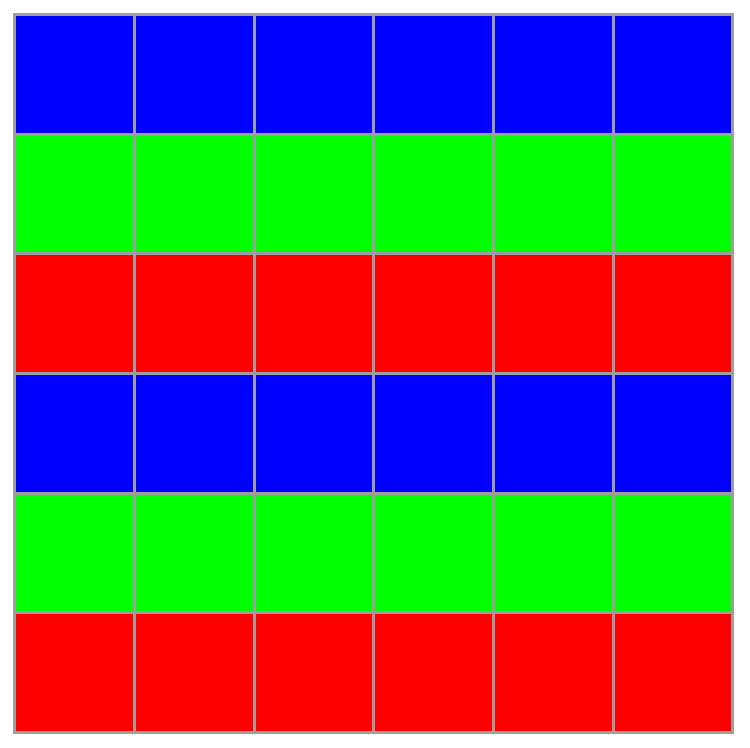
\includegraphics[width=1.0\textwidth]{HL130Block}\\(b)
            \end{center}\end{minipage}
            \hskip 4ex
            \begin{minipage}[c]{0.25\textwidth}\begin{center}
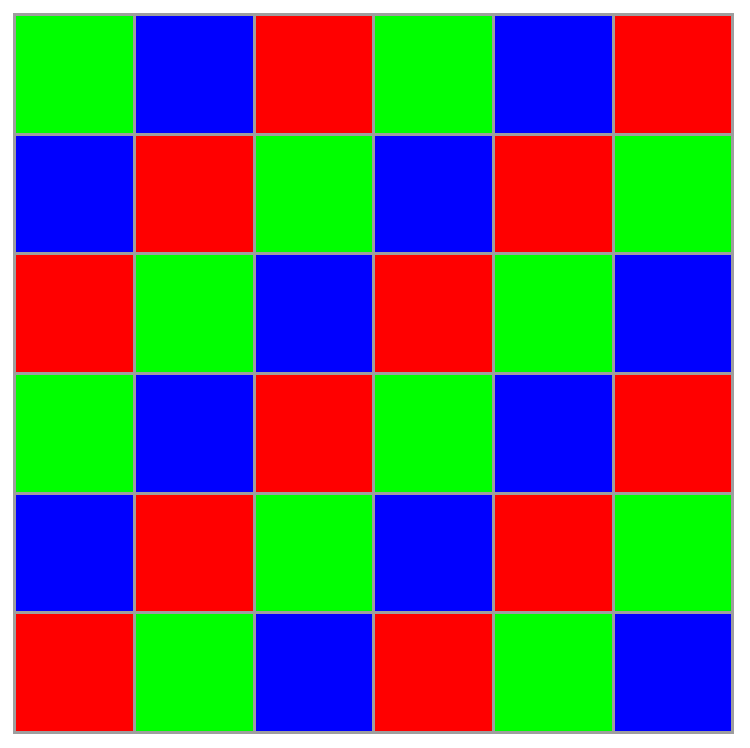
\includegraphics[width=1.0\textwidth]{HL311Block}\\(c)
            \end{center}\end{minipage}
\end{center}
  \caption{\label{fig:SpecialBravaisLatt}
Examples of $\LTS{}{}{}$ periodic \brick s
together with their \spt\ Bravais lattice tilings \refeq{2DBravaisLattice}.
(a)
$\BravCell{3}{1}{0}$, basis vectors
$\mathbf{a}_1=\{3,0\}$ and $\mathbf{a}_2=\{0,1\}$;
(b)
$\BravCell{1}{3}{0}$, basis vectors
$\mathbf{a}_1=\{1,0\}$ and $\mathbf{a}_2=\{0,3\}$;
(c)
$\BravCell{3}{1}{1}$, basis vectors
$\mathbf{a}_1=\{3,0\}$ and $\mathbf{a}_2=\{1,1\}$;
}
\end{figure}
%%%%%%%%%%%%%%%%%%%%%%%%%%%%%%%%%%%%%%%%%%%%%%%%%%%%%%%%%%%%%%%

%%%%%%%%%%%%%%%%%%%%%%%%%%%%%%%%%%%%%%%%%%%%%%%%%%%%%%%%%%%%%
% HL 2020-06-09 siminos/figSrc/han/Mathematica/ColorBlock.nb
\begin{figure}\begin{center}
            \begin{minipage}[c]{0.25\textwidth}\begin{center}
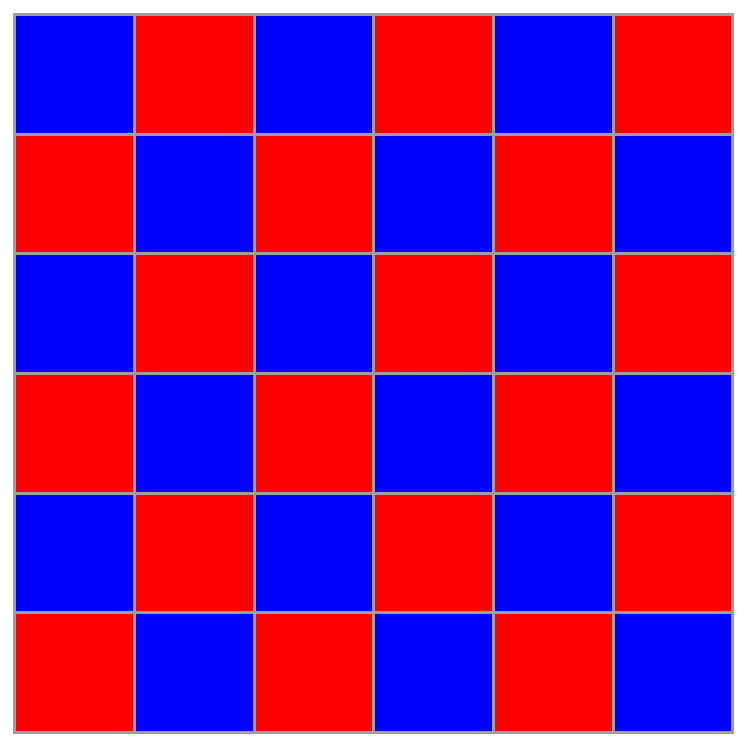
\includegraphics[width=1.0\textwidth]{HL211Block}\\(a)
            \end{center}\end{minipage}
            \hskip 4ex
            \begin{minipage}[c]{0.25\textwidth}\begin{center}
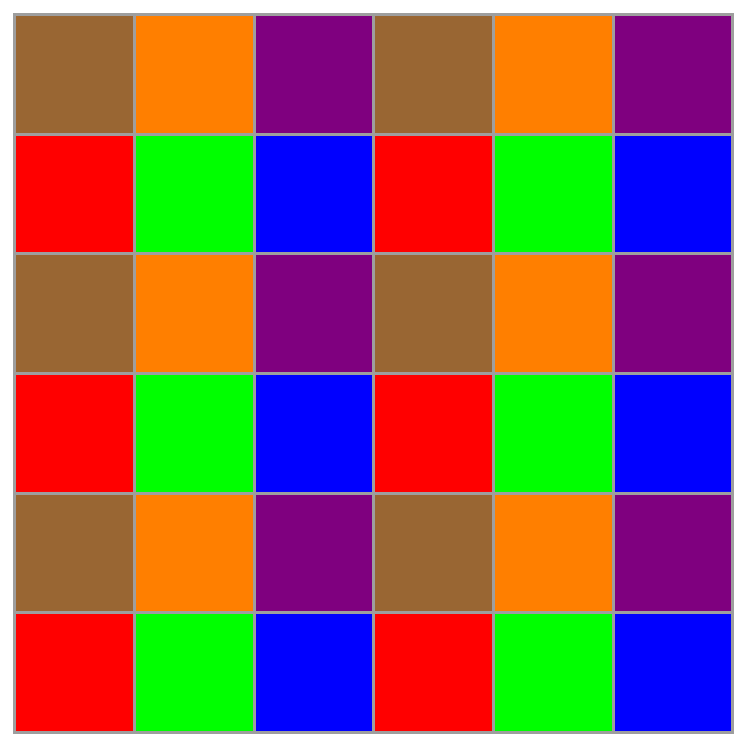
\includegraphics[width=1.0\textwidth]{HL320Block}\\(b)
            \end{center}\end{minipage}
            \hskip 4ex
            \begin{minipage}[c]{0.25\textwidth}\begin{center}
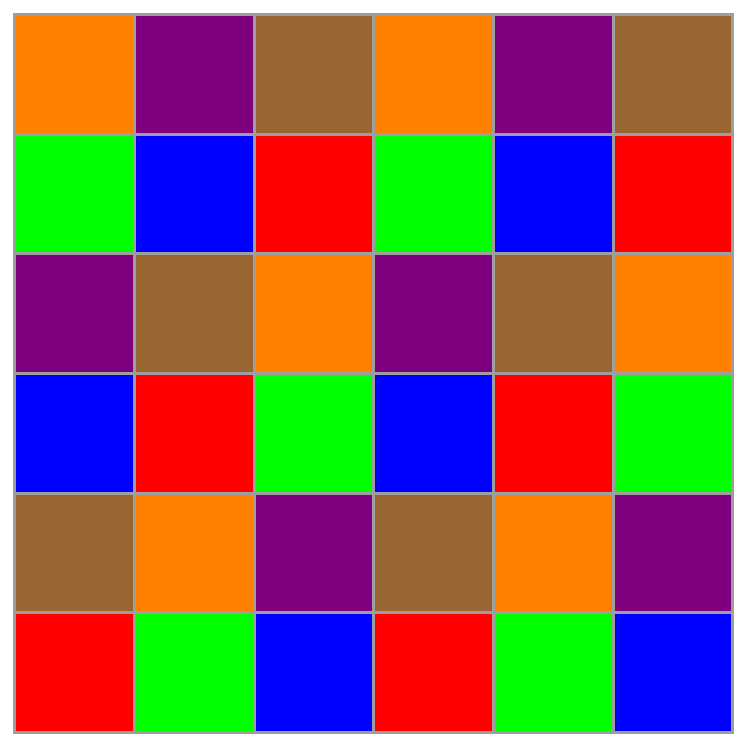
\includegraphics[width=1.0\textwidth]{HL321Block}\\(c)
            \end{center}\end{minipage}
\end{center}
  \caption{\label{fig:3x2rpo}
Examples of $\LTS{}{}{}$ periodic \brick s
together with their \spt\ Bravais lattice tilings \refeq{2DBravaisLattice}.
(a)
$\BravCell{2}{1}{1}$, basis vectors
$\mathbf{a}_1=\{2,0\}$ and $\mathbf{a}_2=\{1,1\}$;
(b)
$\BravCell{3}{2}{0}$, basis vectors
$\mathbf{a}_1=\{3,0\}$ and $\mathbf{a}_2=\{0,2\}$;
(c)
$\BravCell{3}{2}{1}$, basis vectors
$\mathbf{a}_1=\{3,0\}$ and $\mathbf{a}_2=\{1,2\}$;
}
\end{figure}
%%%%%%%%%%%%%%%%%%%%%%%%%%%%%%%%%%%%%%%%%%%%%%%%%%%%%%%%%%%%%%%



    \PCpost{2019-11-23}{
We always reduce relative-shift symmetries, so I am not happy about the
$\BravCell{2}{1}{1}$ relative-periodic {\brick} \refeq{eq:block2x1rp} being
counted as the $\BravCell{2}{2}{0}$ \twot. We'll have to revisit symmetry
reduction...
    }

    \PCpost{2019-11-23}{
For uses of the lexical ordering, ChaosBook table
\toChaosBook{section.18.2}
{18.1:} {\em {\Orbit}s for the binary symbolic dynamics up to length 9},
and appendix
\toChaosBook{section.R.2}
{A18.2} {\em Prime factorization for dynamical itineraries}
might be of interest.

In the paper, we will probably first review the \templatt\ counting,
something along the lines of the above tables.

suggestion of
constructing covering prime \brick s wildly overcounts the candidates for
\admissible\ prime \twots, so we should give up this avenue of
constructing them - no need to count any larger Bravais lattices.
    }


	\HLpost{2020-03-17}{
\emph{PrimeTiles.nb} generates all prime tiles that can tile a
larger tile. It gives
some not obvious results. For example, let the large tile be
$\BravCell{3}{2}{1}$, and consider the full-shift 9-symbol
$\BravCell{3}{2}{1}$ \brick s. The number $\BravCell{3}{2}{0}$ \brick s is
given by \refeq{catlattN3x2}. The program shows that the
$\BravCell{3}{2}{0}$ tile can only be tiled by $\BravCell{1}{1}{0}$,
$\BravCell{1}{2}{0}$ and $\BravCell{3}{1}{0}$ tiles. So we get the result in
\refeq{catlattN3x2}:
\[
N_{\BravCell{3}{2}{0}} = 9^{3\times2} =
88440\,\BravCell{3}{2}{0}+240\,\BravCell{3}{1}{0}
  +36\,\BravCell{1}{2}{0}+9\,\BravCell{1}{1}{0}
\,.
\]
For the full-shift the number of periodic \brick s is given
by the area of the larger tile, and number of $\BravCell{3}{2}{\tilt{}}$ \brick
s is the same for all $S$. But now
$\BravCell{3}{1}{0}$ tile cannot tile the $\BravCell{3}{2}{1}$ tile.
Instead, the $\BravCell{3}{2}{1}$ can be tiled by
$\BravCell{1}{1}{0}$, $\BravCell{3}{1}{2}$  and $\BravCell{1}{2}{0}$ tiles,
 \[
N_{\BravCell{3}{2}{1}} = 9^{3\times2} =
88440\,\BravCell{3}{2}{1}+ 240\,\BravCell{3}{1}{2}+36\,\BravCell{1}{2}{0}
   +9\,\BravCell{1}{1}{0}
\,.
\]
\emph{A priori} is not obvious that $\BravCell{3}{1}{2}$ tile can tile a
$\BravCell{3}{2}{1}$ tile. But if you stack $\BravCell{3}{1}{2}$ tile in the
shifted temporal direction by 2 then the left edge of the tile is shifted
by 4 in the spatial direction. With the spatial period being 3, shifted
by 4 in the spatial direction is same as shifted by 1. So the \bcs\ of
$\BravCell{3}{2}{1}$ tile are satisfied by the $\BravCell{3}{1}{2}$ tiles.
    }


\end{description}


%%%%%%%%%%%%%%%%%%%%%%%%%%%%%%%%%%%%%%%%%%%%%%%%%%%%%%%%%%%%%%%%%%%%%%%
%\printbibliography[heading=subbibintoc,title={References}]

    \ifboyscout\clearpage\fi
% siminos/kittens/Hill.tex      pdflatex CL18
% $Author: predrag $ $Date: 2020-12-23 14:59:59 -0500 (Wed, 23 Dec 2020) $

\section{{\HillDet}:
            stability of an orbit vs. its time-evolution stability}
\label{s:Hill}

The $d=2$ lattice \catlatt\ equations can be recast in a matrix form, by
rewriting the defining equations in terms of \emph{block
matrices}\rf{Dorr70,BuGoNi70,ChenM87,HuRyCo98}, constructed by the
\HREF{https://en.wikipedia.org/wiki/Kronecker_product} {Kronecker
product} $\mathbf{A}\otimes\mathbf{B}$, an operation
(introduced by Zehfuss in 1858) that replaces the $a_{ij}$
element of an [$n\times{n}$] matrix $\mathbf{A}$ by [$m\times{m}$]
matrix block $a_{ij}\mathbf{B}$, resulting in an [$mn\times mn$] block
matrix\rf{ArWeHa13,wikiKronProd}
\beq
\mathbf{A}\otimes\mathbf{B} =
\left[\begin{array}{ccc} %\begin{bmatrix}
  a_{11} \mathbf{B} & \cdots & a_{1n}\mathbf{B} \\
             \vdots & \ddots &           \vdots \\
  a_{n1} \mathbf{B} & \cdots & a_{nn} \mathbf{B}
\end{array}\right] %\end{bmatrix}
\,.
\ee{KronProd}
Consider $\mathbf{A}$, $\mathbf{A'}$ square matrices of size
[$n\times{n}$], and $\mathbf{B}$, $\mathbf{B'}$ square matrices of size
[$m\times{m}$].
The matrix product of two block matrices is a block
matrix\rf{ArWeHa13,wikiBlockMat},
\beq
(\mathbf{A}\otimes\mathbf{B})\,(\mathbf{A'}\otimes\mathbf{B'})
%= (\mathbf{A}\mathbf{A'})\otimes(\mathbf{B}\mathbf{D})
%  {\displaystyle (\mathbf {A} \otimes \mathbf {B} )(\mathbf {C} \otimes \mathbf {D} )
  =(\mathbf{AA'})\otimes (\mathbf{BB'})
  \,.
\ee{mixedProd}
The trace and the determinant of a block matrix are given by
\bea
\tr(\mathbf {A} \otimes \mathbf {B})
    &=& \tr\mathbf{A}\,\tr\mathbf{B}
    \continue
\det\left(\mathbf{A} \otimes \mathbf{B}\right)
    &=& \det\left(\mathbf{A}^{m}\right) \det\left(\mathbf{B}^{n}\right)
\,.
\label{wikiKron2}
\eea
The two [$mn\times mn$] block matrices $\mathbf{A}\otimes\mathbf{B}$ and
$\mathbf{B}\otimes\mathbf{A}$ are equivalent by a similarity
transformation
\beq
\mathbf {B} \otimes \mathbf {A}
=\transp{\mathbf {P}} \,(\mathbf {A} \otimes \mathbf {B} )\,\mathbf {P}
\,,
\ee{wikiKron3}
where $\mathbf{P}$ is permutation matrix. As $\det{\mathbf{P}}=1$,
the block matrix determinant
$\det\left(\mathbf{A}\otimes\mathbf{B}\right)
=
\det\left(\mathbf{B}\otimes\mathbf{A}\right)$
is independent of the order in which blocks are constructed.

Consider a rectangular $d=2$ lattice
$\BravCell{\speriod{}}{\period{}}{0}$ Bravais cell. The \jacobianOrb\
\refeq{catLatt} written as a
$[\speriod{}\period{}\times\speriod{}\period{}]$ Kronecker product block
matrix is
\beq
\jMorb
=
\id_{1} \otimes \left(\hopMat_{2}+\hopMat_{2}^{-1}\right)
-
2 {s}\,\id_1\otimes\id_{2}
+
\left(\hopMat_{1}+\hopMat_{1}^{-1}\right) \otimes \id_{2}
\,,
\ee{catalattLxT}
where the \refeq{KronProd} matrix $\mathbf{A}$ and identity
$\id_1$ matrix are `spatial' [$\speriod{}\!\times\!\speriod{}$]
matrices, with blocks $\mathbf{B}$ and identity $\id_2$ `temporal'
[$\period{}\!\times\!\period{}$] matrix blocks. Indices `1', `2'
referring to `spatial', `temporal' lattice directions, respectively.

Our task is to compute the {\HillDet} $|\det \jMorb|$. We first show how
to do that directly, by computing the volume of the {\fundPip}.

\subsection{{\HillDet}: fundamental parallelepiped evaluation}
\label{s:catLattRel3x2}
% 2020-02-16 Predrag computed  using siminos/mathematica/Tensors.nb
As a concrete example
consider the Bravais lattice \refeq{2DBravaisLattice} with basis
vectors $\mathbf{a}_1=(3,0)$ and $\mathbf{a}_2=(0,2)$. A \twot\ over this
Bravais cell has 6 field values, one for each lattice site $z=(n,\zeit)$
on a $\BravCell{3}{2}{0}$ rectangle:
\[
 \left[\begin{array}{ccc}
 \ssp_{01} & \ssp_{11} & \ssp_{21} \\
 \ssp_{00} & \ssp_{10} & \ssp_{20}
 \end{array}\right]
\,.
\]
Stack up the columns of this lattice state and the corresponding sources
into 6\dmn\ vectors,
\beq
\Xx_{\BravCell{3}{2}{0}} =
\left(\begin{array}{c}
 \ssp_{01} \\
 \ssp_{00} \\
  \hline
 \ssp_{11} \\
 \ssp_{10} \\
  \hline
 \ssp_{21} \\
 \ssp_{20} \\
      \end{array}\right)
\,,\qquad
\Mm_{\BravCell{3}{2}{0}} =
\left(\begin{array}{c}
 \Ssym{01} \\
 \Ssym{00} \\
  \hline
 \Ssym{11} \\
 \Ssym{10} \\
  \hline
 \Ssym{21} \\
 \Ssym{20} \\
        \end{array}\right)
\,.
\ee{3times2blockVect}
The corresponding {\jacobianOrb} \refeq{catlattFix}
%\([\BravCell{3}{2}{}\times \BravCell{3}{2}{}]\)
%4-index matrix $\jMorb_{zz'}$.
is the  block-matrix
\refeq{catalattLxT},
a block circulant matrix
with circulant blocks\rf{ChenM87},
\beq
\jMorb_{\BravCell{3}{2}{0}} =
\left(
\begin{array}{cc|cc|cc}
 -2 s & 2 & 1 & 0 & 1 & 0  \\
 2 & -2 s & 0 & 1 & 0 & 1  \\
  \hline
 1 & 0 & -2 s & 2 & 1 & 0  \\
 0 & 1 & 2 & -2 s & 0 & 1  \\
  \hline
 1 & 0 & 1 & 0 & -2 s & 2  \\
 0 & 1 & 0 & 1 & 2 & -2 s
\end{array}
\right)
\,.
\ee{3times2blockMat}
of $[\speriod{}\!\times\!\speriod{}]$ block form, $\speriod{}=3$,
with $[\period{}\!\times\!\period{}]$ blocks, $\period{}=2$.

The {\fundPip} generated by the action of {\jacobianOrb}
$\jMorb_{\BravCell{3}{2}{0}}$ is spanned by $\speriod{}\period{}=6$ basis
vectors, the columns \refeq{lattJac} of the {\jacobianOrb}
\refeq{3times2blockMat}:
\beq
\jMorb_{\BravCell{3}{2}{0}} =
\left(
\begin{array}{c|c|c|c|c|c}
 -2 s & 2 & 1 & 0 & 1 & 0  \\
 2 & -2 s & 0 & 1 & 0 & 1  \\
 1 & 0 & -2 s & 2 & 1 & 0  \\
 0 & 1 & 2 & -2 s & 0 & 1  \\
 1 & 0 & 1 & 0 & -2 s & 2  \\
 0 & 1 & 0 & 1 & 2 & -2 s
\end{array}
\right)
\,.
\ee{3times2basisVecs}
The `fundamental fact' \refeq{detBern0} now yields the {\HillDet}
as the number of
doubly-periodic lattice states,
\beq
N_{\BravCell{3}{2}{0}} = |\Det\jMorb_{\BravCell{3}{2}{0}}|
                   = 4({s}-2)s(2{s}-1)^2 (2{s}+3)^2
\,.
\ee{N3times2}

\subsection{{\HillDet}: time-evolution evaluation}
\label{s:HillHam}

In practice, one often
computes the {\HillDet} using a  Hamiltonian, or `transfer matrix'
formulation. An example is the \templatt\ 3-term recurrence
\refeq{catMapNewt},
\bea
\ssp_{\zeit}
&=& ~~\ssp_{\zeit}
    \continue
\ssp_{\zeit+1}
&=&  - \ssp_{\zeit-1} +{s} \, \ssp_{\zeit} - \Ssym{\zeit}
\,,
\nnu
\eea
in the \PV\rf{PerViv} `two-configuration' cat map
representation \refeq{eq:StateSpCatMap}
\beq
 \hat{\xx}_{\zeit+1} =
      {\hat{\mathbf{\jMat}}_1}\,\hat{\xx}_\zeit - \hat{\mathsf{\Ssym{}}}_\zeit
\,,
\ee{PV2config}
with the one-time step temporal evolution
[$2\!\times\!2$] {\jacobian} matrix
${\hat{\mathbf{\jMat}}_1}$ generating a time orbit by acting on the
2\dmn\ `phase space' of states on successive lattice sites
\beq
 {\hat{\mathbf{\jMat}}_1}
=
 \left[\begin{array}{cc}
 0 & 1 \\
 -1 & s
 \end{array} \right]
\,,\qquad
\hat{\xx}_\zeit
=
\left[\begin{array}{c}
 \ssp_{\zeit-1}\\
 \ssp_{\zeit}
\end{array}\right]
\,,\qquad
\hat{\mathsf{\Ssym{}}}_\zeit
=
\left[\begin{array}{c}
 0           \\
 \Ssym{\zeit}
\end{array}\right]
\,,
\ee{PV2configJ}
Similarly, for the $d=2$ \catlatt\ lattice at hand, one can
recast the 5-term recurrence \refeq{CatMap2d}
\bea
\ssp_{n\zeit}
&=& ~~\ssp_{n\zeit}
%(- \ssp_{n+1,\zeit-1} + 2{s} \, \ssp_{n,\zeit-1} - \ssp_{n-1,\zeit-1})
%- \Ssym{n,\zeit-1}
%- \ssp_{n,\zeit-2}
    \continue
\ssp_{n,\zeit+1}
&=&  - \ssp_{n,\zeit-1}
 +(- \ssp_{n-1,\zeit} + 2{s} \, \ssp_{n\zeit} - \ssp_{n+1,\zeit})
- \Ssym{n\zeit}
%\,,
\label{CatMap2dHill}
\eea
in the `two-configuration' matrix form \refeq{PV2config} by picking the
vertical direction (indexed `2') as the `time', with temporal 1-time step {\jacobian}
[$2\speriod{}\!\times\!2\speriod{}$] block matrix
% ${\hat{\mathbf{\jMat}}_1}$
\beq
{\hat{\mathbf{\jMat}}_1}  =
 \left[\begin{array}{c|c}
{\bf 0} & \id_1\\ \hline
-\id_1 & {-\mathbf{\jMorb}_1}
 \end{array} \right]
\,,
\ee{PV2catlattJ}
(known as a transfer matrix in statistical
mechanics\rf{Onsager44,MonMun94}) generating a `time' orbit by acting on a
$2\speriod{}$\dmn\ `phase space'  lattice strip
$\hat{\xx}_\zeit$ along the `spatial' direction  (indexed `1'),
\[  %\beq
\hat{\xx}_\zeit
=
\left[\begin{array}{c}
 {\xx}_{\zeit-1}\\ \hline
 {\xx}_\zeit
 \end{array}\right]
,\quad
\hat{\mathsf{\Ssym{}}}_\zeit
=
    \left[\begin{array}{c}
    \mathbf{0}\\ \hline
 \mathsf{\Ssym{}}_{\zeit}
 \end{array}\right]
,\qquad
\xx_\zeit
=
\left[\begin{array}{c}
 \ssp_{1\zeit}\\   \vdots\\ \ssp_{\speriod{}\zeit}
 \end{array}\right]
,\quad
\mathsf{\Ssym{}}_\zeit
=
    \left[\begin{array}{c}
 \Ssym{1\zeit}\\ \vdots\\ \Ssym{\speriod{}\zeit}
 \end{array}\right]
,
\] %\ee{PV2catlattJ1}
where the hat $\hat{~}$~ indicates a $2\speriod{}$\dmn\
`two-configuration' state, and $\mathbf{\jMorb}_1$ is the spatial
$[\speriod{}\!\times\!\speriod{}]$ {\jacobianOrb} of
$d=1$ \templatt\ form \refeq{tempCatFix},
\beq
\mathbf{\jMorb}_1
        =
\hopMat_{1}^{-1} - 2s \id_1 + \hopMat_{1}
\label{Hessian_Hill}
\eeq
The `two-configuration' coupled cat maps system \refeq{PV2config} is a
generalization of the Bernoulli map time evolution formulation
\refeq{tempBern} to a high-dimensional spatially-coupled lattice. Just as
in the {temporal Bernoulli} condition \refeq{tempFixPoint}, the first
order in time difference equation \refeq{PV2config} can be viewed as a
lattice state fixed point condition \refeq{tempFixPoint}, a zero of the
function
\( %beq
F[\hat{\Xx}] = \hat{\mathbf{\jMorb}}\hat{\Xx}+\hat{\Mm} = 0
\,,
\) %\ee{tempPV2Point}
with the entire periodic \emph{lattice state} $\hat{\Xx}_{\Mm}$ treated as a
single fixed \emph{point} in the
$2\speriod{}\period{}$\dmn\ \statesp\ unit hyper-cube, and the
$[2\speriod{}\period{}\times2\speriod{}\period{}]$  block matrix \jacobianOrb\
given either by
\beq
\hat{\mathbf{\jMorb}} =
    \hat{\id} - {\hat{\mathbf{\jMat}}_1}\otimes\hopMat_2^{-1}
\,,
\ee{tempPV2conf12}
or by
\beq
\hat{\mathbf{\jMorb}}' =
    \hat{\id} -\hopMat_2^{-1} \otimes {\hat{\mathbf{\jMat}}_1}
\,.
\ee{tempPV2conf21}
Here the unity $\hat{\id}=\hat{\id}_1\otimes\id_{2}$ is a
[$2\speriod{}\period{}\!\times\!2\speriod{}\period{}$] block matrix, and
the time-evolution \jacobianM\ ${\hat{\mathbf{\jMat}}_1}$
\refeq{PV2catlattJ} is a [$2\speriod{}\!\times\!2\speriod{}$] matrix.

The order in which the block matrix blocks are composed does not matter,
yielding the same the {\HillDet} $\det\hat{\mathbf{\jMorb}} =
\det\hat{\mathbf{\jMorb}}'$ by \refeq{wikiKron3}.
However, written out explicitly, the two \jacobianOrbs\
\refeq{eq:orbitJPVJxS} and \refeq{eq:orbitJPVtempJ} are of a very
different form.

For example, for the $\BravCell{\speriod{}}{\period{}}{0}$  rectangular
Bravais cell, the \catlatt\ \jacobianOrb\ \refeq{tempPV2conf12} involves the
[$\period{}\!\times\!\period{}$] time {\shiftOp} block matrix $\hopMat_2$
\refeq{hopMatrix} with the one-time-step [$2\speriod{}\!\times\!2\speriod{}$]
time-evolution \jacobianM\ ${\hat{\mathbf{\jMat}}_1}$ \refeq{PV2catlattJ}
\bea
\hat{\mathbf{\jMorb}}
    &=&
\left[\begin{array}{c|c}
 \id_{1}\otimes\id_{2}   & -\id_1\otimes\hopMat_2^{-1}             \\ \hline
 \id_1\otimes\hopMat_2^{-1}& \id_{1}\otimes\id_{2} +\mathbf{\jMorb}_1\otimes\hopMat_2^{-1}
\end{array}\right]
\,,
\label{eq:orbitJPVJxS}
\eea
and for \catlatt\ \refeq{CatMap2dHill} this is a time-periodic
[$\period{}\times\period{}$]  {\shiftOp} block matrix $\hopMat_2$
\refeq{hopMatrix}, each block now a space-periodic
[$2\speriod{}\!\times\!2\speriod{}$] matrix ${\hat{\mathbf{\jMat}}_1}$
\refeq{PV2catlattJ}.

If a block matrix is composed of four blocks,
\HREF{https://en.wikipedia.org/wiki/Block_matrix\#Block_matrix_inversion}
{its determinant} can be evaluated using Schur's 1917
formula\rf{Schur1917,wikiBlockMat}
%From \refeq{det2x2blockMat*** we have
\beq
\det\left[\begin{array}{c|c}
\mathbf{A} & \mathbf{B} \\ \hline
\mathbf{C} & \mathbf{D}
\end{array}\right]
=
\det(\mathbf{A})\,\det(\mathbf{D}-\mathbf{C}\mathbf{A}^{-1}\mathbf{B})
\,.
\ee{det2x2blockMat}
so, noting \refeq{mixedProd}, \refeq{catalattLxT} and
\refeq{Hessian_Hill}, we find that
\bea
\det\hat{\mathbf{\jMorb}}
    &=&
\det\left[\begin{array}{c|c}
 \id_{1}\otimes\id_{2}   & -\id_1\otimes\hopMat_2^{-1}             \\ \hline
 \id_1\otimes\hopMat_2^{-1}& \id_{1}\otimes\id_{2} +\mathbf{\jMorb}_1\otimes\hopMat_2^{-1}
\end{array}\right]
     \continue
     &=&
% \det(\id_1)\,
\det\left[
       \id_{1}\otimes\id_{2} + \mathbf{\jMorb}_1\otimes\hopMat_2^{-1}
     + (\id_1\otimes\hopMat_2^{-1})(\id_{1}\otimes\id_{2})(\id_1\otimes\hopMat_2^{-1})
    \right]
     \continue
     &=&
\det\left[
       \id_{1}\otimes\id_{2} + \mathbf{\jMorb}_1\otimes\hopMat_2^{-1}
     +  \id_1\otimes\hopMat_2^{-2}
    \right]
     \continue
     &=&
\det(\id_1\otimes\hopMat_2^{-1})\,
\det\left[
       \id_1\otimes\hopMat_2^{-1}
        +(\hopMat_{1}^{-1} - 2s \id_1 + \hopMat_{1})\otimes\id_2
     +  \id_1\otimes\hopMat_2
    \right]
     \continue
     &=&
\det \jMorb
\,,
\label{det2x2blockMat2LH}
\eea
where we have used
$\det\id_{1}=\det\id_{2}=\det\hopMat_{1}=\det\hopMat_{2}=1$.

This proves that $\det\hat{\mathbf{\jMorb}}$ of the
`Hamiltonian' or `two-configuration'
$[2\speriod{}\period{}\times2\speriod{}\period{}]$ `phase space'
\jacobianOrb\ $\hat{\mathbf{\jMorb}}$ defined by \refeq{eq:orbitJPVJxS}
equals the `Lagrangian' {\HillDet} of the
$[\speriod{}\period{}\times\speriod{}\period{}]$ \jacobianOrb\
$\mathbf{\jMorb}$.

\subsection{Hill's formula}
\label{s:HillForm}

Consider next \refeq{tempPV2conf21}, the equivalent way of forming of the
block matrix for the $\BravCell{\speriod{}}{\period{}}{0}$  rectangular
Bravais cell, with temporal period taken for definitiveness
$\period{}=4$. The \catlatt\ \jacobianOrb\ \refeq{tempPV2conf21} is now
constructed as the [$4\times4$] time {\shiftOp} block matrix $\hopMat_2$
\refeq{hopMatrix}, with the one-time-step
[$2\speriod{}\!\times\!2\speriod{}$] time-evolution \jacobianM\
${\hat{\mathbf{\jMat}}_1}$ \refeq{PV2catlattJ} and unit matrix
$\hat{\id}_1$ as blocks
\beq
\hat{\mathbf{\jMorb}}'
 =
\id_2\otimes\hat{\id}_{1} -\hopMat_2^{-1} \otimes {\hat{\mathbf{\jMat}}_1}
 =
\left[\begin{array}{c|c|c|c}
 \hat{\id}_1    &  {\bf 0}   & {\bf 0}    &-{\hat{\mathbf{\jMat}}_1} \\ \hline
-{\hat{\mathbf{\jMat}}_1} &  \hat{\id}_1   & {\bf 0}    & {\bf 0}    \\ \hline
 {\bf 0}    &-{\hat{\mathbf{\jMat}}_1} & \hat{\id}_1    & {\bf 0}    \\ \hline
 {\bf 0}    &  {\bf 0}   &-{\hat{\mathbf{\jMat}}_1} & \hat{\id}_1
\end{array}\right]
\,.
\label{eq:orbitJPVtempJ}
\eeq
The {\HillDet} $\det\hat{\mathbf{\jMorb}}'$ evaluation follows
essentially the same path as the Bernoulli {\HillDet} evaluation of
\refsect{s:bernCount}, generalized to block matrices. From the
block-matrix multiplication rule \refeq{mixedProd} and the determinant
rule \refeq{wikiKron2} it follows that
\beq
(\hopMat_2^{-1}\otimes{\hat{\mathbf{\jMat}}_1})
(\hopMat_2^{-1}\otimes{\hat{\mathbf{\jMat}}_1})
=
\hopMat_2^{-2}\otimes{\hat{\mathbf{\jMat}}_1}^2
\,,\quad\mbox{ so }
(\hopMat_2^{-1} \otimes {\hat{\mathbf{\jMat}}_1})^k =
\hopMat_2^{-k} \otimes {\hat{\mathbf{\jMat}}_1}^k
\,,
\ee{shiftPower}
and
\beq
\det(\hopMat_2^{-1}\otimes{{\hat{\mathbf{\jMat}}_1}})
=
(\det\hopMat_2)^{-\speriod{}}
(\det{\hat{\mathbf{\jMat}}_1})^\period{}
=
\det\hat{\mathbf{\jMat}}_p
\,,\qquad
\hat{\mathbf{\jMat}}_p = {\hat{\mathbf{\jMat}}_1}^\period{}
\,,
\ee{detShiftxJ}
where $\hat{\mathbf{\jMat}}_p$ is the {\jacobianM} of a
temporal periodic orbit $p$.
Expand
\(
 \ln\det\hat{\mathbf{\jMorb}}'
   =
 \tr\ln\hat{\mathbf{\jMorb}}'
\)
as a series using \refeq{wikiKron2} and \refeq{shiftPower},
\beq
\tr\ln\hat{\mathbf{\jMorb}}' =
\tr\ln(\id-\hopMat_2^{-1} \otimes {{\hat{\mathbf{\jMat}}_1}})
  =
-\sum_{k=1}^\infty\frac{1}{k}{\tr(\hopMat_2^{-k})}\,\tr{{\hat{\mathbf{\jMat}}_1}}^{k}
\,,
\ee{LnDet=TrLn_Hill}
and use
$\tr \hopMat_2^k=\period{}$
if $k$ is a multiple of $\period{}$,
0 otherwise
(follows from $\hopMat_2^\period{}=\id$):
\[
\ln\det(\id-\hopMat_2^{-1} \otimes {{\hat{\mathbf{\jMat}}_1}})
  =
-\sum_{r=1}^\infty\frac{1}{r}\tr\hat{\mathbf{\jMat}}_p^{r}
  =
\ln\det(\hat{\id}_{1}-\hat{\mathbf{\jMat}}_p)
\,.
\]
So for the {\catlatt} the {\jacobianOrb}  and the temporal evolution
\refeq{PV2config} stability ${{\hat{\mathbf{\jMat}}_{p}}}$ are related by
the remarkable (discrete time) Hill's formula\rf{MacMei83,BolTre10}
\beq
|\det\jMorb|
  =
|\det(\hat{\id}_{1}-\hat{\mathbf{\jMat}}_p)|
\,.
\ee{HillDet}
which expresses the  {\HillDet} of the arbitrarily large \jacobianOrb\
$\jMorb$  in terms of a determinant of a small
[$2\speriod{}\!\times\!2\speriod{}$] time-evolution \jacobianM\
$\hat{\mathbf{\jMat}}_p$.


\bigskip

Two remarks.
First, the reformulation of the \catlatt\ 5-term recurrence
\refeq{CatMap2dHill} as the `two-configuration' form \refeq{PV2config} is
a passage from the Lagrangian to the Hamiltonian formulation, also known
as `transfer matrix' formulation of lattice field
theories\rf{MonMun94,MunWal00} and Ising
models\rf{Onsager44,Kastening02}. We chose to prove it here using only
elementary linear algebra, not only because the Lagrangian
formalism\rf{BolTre10} is not needed for the problem at hand, but because
it actually obscures the generality of Hill's formula, which works
equally well for dissipative systems (see Bernoulli Hill's formula
\refeq{noPerPts}), systems with no Lagrangian formulation.

Second,
for Hamiltonian evolution \refeq{catMap}, the $[2\!\times\!2]$
\jacobianM\ $\jMat^\period{}$ (the monodromy matrix of a \po) describes
the growth of an initial state perturbation in $\period{}$ steps. For the
corresponding Lagrangian system with action $\action$,
% (see \refsect{s:catLagrForm}),
the first variation of
the action $\delta\action=0$ yields the \templatt\ condition
\refeq{catTempLatt}, while the second variation, the
$[\period{}\!\times\!\period{}]$ {\jacobianOrb} \refeq{tempCatFix},
describes the stability of the \emph{entire} given \po. In this,
classical mechanics context, Bolotin and Treschev\rf{BolTre10} refer to
$\jMorb$ as the `Hessian operator', but, as it is clear from our
Bernoulli discussion of \refsect{s:JacobianOrb}, and applications to \KS\
and Navier-Stokes systems\rf{GuBuCv17}, this notion of global stability
of orbits is general, and applies to all dynamical systems, not only the
Hamiltonian ones.

Accordingly, by the discrete time Hill's formula \refeq{HillDet}, just as
for the Bernoulli example \refeq{detDet} these two expressions are
equivalent,
\beq
|\Det\jMorb_\Mm| = |\det(\id-\jMat_\Mm)|
\,.
\ee{detDetCat}
As the cat map hyperbolicity is the same everywhere and
does not depend on a particular solution $\Xx_p$, counting \po s is all
that is needed to solve a cat-map dynamical system completely; once \po s
are counted, all {\cycForm s}\rf{CBtrace} follow.

    \ifboyscout\clearpage\fi
% siminos/spatiotemp/chapter/summary.tex
% $Author: predrag $ $Date: 2019-10-24 23:59:13 -0400 (Thu, 24 Oct 2019) $

%\section{Summary}
%\label{sect:summary}
% Predrag copied from siminos/rpo_ks/current/summary.tex    2019-05-15

\refRef{SCD07} studied the \KS\ flow as a staging ground for
testing dynamical systems approaches to
moderate Reynolds number turbulence in full-fledged
({\em not} a few-modes model),
infinite-dimensional \statesp\ PDE settings\rf{Holmes96},
and present a detailed geometrical portrait of dynamics in the
{\KS} \statesp\ for the $L=22$ system size, the smallest
system size for which this system empirically exhibits
`sustained turbulence.'

Compared to the earlier work
\rf{Christiansen97,LanThesis,lanCvit07,lop05rel},
the main advances here are the new insights in
the role that continuous symmetries,
discrete symmetries,
low-dimensional unstable manifolds of \eqva,
and the connections between \eqva\ play in organizing the flow.
The key new feature of the translationally invariant KS
on a periodic domain
are the attendant continuous families of
\reqva\ (traveling waves) and \rpo s.
We have now understood the preponderance of solutions of
relative type, and lost fear of them:
a large number of unstable \rpo s and \po s has been determined
here numerically.

Visualization of infinite-dimensional
\statesp\ flows, especially in presence of continuous symmetries,
is not straightforward.
\refRef{SCD07} offered two low-dimensional visualizations of such
flows: (1) projections onto 2- or 3-dimensional,
PDE representation independent
dynamically invariant frames, and
(2) projections onto
the physical, symmetry invariant but time-dependent
energy transfer rates.

\Rpo s require a reformulation of the periodic orbit
theory\rf{Cvi07}, as well as a rethinking of the dynamical
systems approaches to constructing symbolic dynamics,
outstanding problems that we hope to address in near future%
\rf{SCD09b,SiminosThesis}.
What we have learned from the $L=22$ system  is that many of
these \rpo s appear organized by the unstable manifold of
$\EQV{2}$, closely following the homoclinic loop formed
between $\EQV{2}$ and $\Shift_{1/4}\EQV{2}$.

In the spirit of the parallel studies of boundary shear flows\rf{HaKiWa95},
the {\KS} $L=22$ system size was chosen as the smallest
system size for which KS empirically exhibits
`sustained turbulence.'
This is convenient both for
the analysis of the \statesp\ geometry, and for the numerical reasons,
 but the price is high - much of the
observed dynamics is specific to this unphysical, externally
imposed periodicity. What needs to be
understood is the nature of \eqv\ and \rpo\ solutions in the
$L \to \infty$ limit, and the structure of the $L = \infty$ periodic orbit
theory.

In summary, {\KS} (and \pCf, see \refref{GHCW07})  \eqva, \reqva, \po s and
\rpo s embody Hopf's vision\rf{hopf48}: together they form the
 repertoire of recurrent spatio-temporal
patterns explored by turbulent dynamics.

%%%%%%%%%%%%%%%%%%%%%%%%%%%%%%%%%%%%%%%%%%%%%%%%%%%%%%%%%%%%%%%%%%%%%%%%%%

\ack
Work of P.~C. was in part supported by the family of late G. Robinson,
Jr..
We are grateful to Sara A. Solla's many perspicacious comments on
this manuscript.
No actual cats, graduate or undergraduate %, have shown interest in, or
were harmed during this research. This paper sets up the necessary
underpinnings for the quantum field theory of \catlatt, the details of
which we leave to our % always trustworthy
friends Jon Keating and Marcos Saraceno.

%%%%%%%%%%%%%%%%%%%%%%%%%%%%%%%%%%%%%%%%%%%%%%%%%%%%%%%%%%%%%%%%%%%%%%%%%%

%    \ifboyscout
%%    \clearpage
%\bigskip\noindent
%    {\scriptsize
%To obtain a simple heading of `Appendix' use the code
%\verb"\section*{Appendix}". If it contains numbered equations, figures or
%tables the command \verb"\setcounter{section}{1}" must follow it.
%    }
%    \fi %end of the internal draft switch

\appendix
    \ifboyscout\clearpage\fi
% siminos/kittens/appeFourier.tex      pdflatex CL18
% $Author: predrag $ $Date: 2021-07-22 01:45:43 -0400 (Thu, 22 Jul 2021) $

\section{Discrete Fourier transforms}
\label{appe:Fourier}

    \PC{2020-07-11}{
As $n$, $\zeit$ are integers, the 2{\dmn} Fourier transform is periodic
with rectangular period $2\pi\times2\pi$, and only needs be calculated
for one period, usually taken to be $[-\pi,\pi]\times[-\pi,\pi]$.
    }

%TEMPORARY
\bigskip



In this appendix we show how compute the {\jacobianOrb} or {\HillDet}s
$|\Det\jMorb|$ using crystallographer's favorite tool, the discrete
Fourier transform.

\subsection{Temporal Bernoulli}

Due to the time-translation invariance of Bernoulli time evolution law
\refeq{1stepDiffEq}, the {\jacobianOrb} $\jMorb=\id-{s}\,\hopMat^{-1}$
is an $[\cl{}\!\times\!\cl{}]$ is a circulant matrix.
A circulant matrix is constant along each diagonal,
\beq
C=
 \left(\begin{array}{ccccc}
c_0     & c_{\cl{}-1} & \dots  & c_{2} & c_{1}  \\
c_{1} & c_0    & c_{\cl{}-1} &         & c_{2}  \\
\vdots  & c_{1}& c_0    & \ddots  & \vdots   \\
c_{\cl{}-2}  &        & \ddots & \ddots  & c_{\cl{}-1}   \\
c_{\cl{}-1}  & c_{\cl{}-2} & \dots  & c_{1} & c_0 \\
          \end{array} \right)
\,,\qquad
C_{jk} = c_{j-k}
\,,
\ee{circulMatr}
diagonalizable by a discrete Fourier transform,
\beq
 U^{\dagger} C U = \mathrm{diag}(\lambda)
\,,\qquad
 U_{jk} = \frac{1}{\sqrt{\cl{}}}\,\epsilon^{(j-1)(k-1)}
\,,
\ee{appe:FourTransMatr}
with discrete Fourier
mode eigenvectors
\beq
\tilde{e}_k =
    \frac{1}{\sqrt{\cl{}}}
    (1, \epsilon^k, \epsilon^{2k}, \ldots, \epsilon^{k(\cl{}-1)})^{\rm T}
    \,,\qquad k=0, 1,\ldots, \cl{}-1
\,,
\ee{appe:FourEigVecs}
and eigenvalues
\(
C \tilde{e}_k=\lambda_k \tilde{e}_k
\,,
\)
\beq
\lambda_k =
    c_0 + c_{\cl{}-1} \epsilon^k + c_{\cl{}-2} \epsilon^{2k} + \ldots
        + c_{1} \epsilon^{k(\cl{}-1)}
\,,
\ee{circulMatrEigs}
where
\beq
\epsilon=\e^{2\pi\mathrm{i}/\cl{}}
\ee{appe:rootUnityCL18}
is an $\cl{}$th root of unity. The eigenvalues of the Bernoulli
{\jacobianOrb} $(\id-{s}\,\hopMat^{-1})$ are given by the nonzero
coefficients $c_0=1$, $c_1=-{s}$,
\beq
\lambda_k=1 - {s}\,\epsilon^{-k}
\,,
\ee{appe:tempBernFT}
with discrete Fourier transform diagonalizing the Bernoulli equation
\refeq{tempBern},
\beq
(\id - {s} \,\hopMat^{-1})\,\tilde{\Xx}_k
= (1 - {s}\,\epsilon^{-k})\,\tilde{\Xx}_k
= - \,\tilde{\Mm}_k
\,,
\ee{tempBernFT}
where the $\tilde{\Xx}_k$ and $\tilde{\Mm}_k$ are the $k$th Fourier modes of the lattice state $\Xx$ and symbol block $\Mm$:
\beq
\tilde{\Xx}_k
= \left(\transp{\tilde{e}_k}\,{\Xx}\right) \tilde{e}_k
\,, \quad
\tilde{\Mm}_k
= \left(\transp{\tilde{e}_k}\,{\Mm}\right) \tilde{e}_k
\,.
\ee{tempBernFTFields}

The total number of the solutions of the fixed point condition
\refeq{tempFixPoint} is given by \refeq{detBern0}, the `fundamental fact'
{\HillDet} $|\Det\jMorb|$, \ie, the product of the {\jacobianOrb}
eigenvalues,
\beq
N_\cl{} = \left| \Det \jMorb \right|
 = \prod_{k=0}^{\cl{}-1}\left| 1 - {s}\,\epsilon^{-k}\right|
 = \prod_{k=0}^{\cl{}-1}\left| {s} - \epsilon^{k}\right|
 = s^{\cl{}} - 1
\,,
\ee{appe:detBern2}
where the last equality follows from $\epsilon^k$ being the $k$th
root of equation ${s}^\cl{}-1=0$, so
\[
{s}^\cl{}-1 = \prod_{k=0}^{\cl{}-1} ({s} - \epsilon^k)
\,.
\] %ee{factorPoly}
This verifies the `fundamental fact' count of Bernoulli solutions
\refeq{detBern2}.

\subsection{\tempLatt}

The \templatt\ \jacobianOrb\
$\jMorb = \hopMat-{s}\,\id+\hopMat^{-1}$ %\refeq{tempCatFix}
is an $[\cl{}\!\times\!\cl{}]$ circulant matrix \refeq{Hessian}, with
eigenvalues  \refeq{circulMatrEigs}
\beq
\lambda_k
= \epsilon^{-k} - {s} + \epsilon^{k}
= - {s} + 2 \cos\left({2\pi k}/{\cl{}}\right)
\,,
\ee{appe:tempCatFT}
and the {\HillDet}
\beq
N_\cl{} = \left| \Det \jMorb \right|
 =
\prod_{k=0}^{\cl{}-1} \left|{s}-2\cos\left({2\pi k}/{\cl{}}\right)\right|
\,.
\ee{appe:detTemCat}
It is not immediately obvious that such products of trigonometric functions
should be integer-valued\rf{Dubout19}, and establishing that usually requires
some work\rf{Wu04}.

In case at hand we observe that as the Chebyshev polynomials of the first
kind\rf{boyd01} satisfy $T_{\cl{}}(\cos(x))=\cos(\cl{}x)$, for $x=2\pi
k/\cl{}$, $k=0,1,...,\cl{}-1$, $\cos(2\pi k/\cl{})$ is the $k$th root of
equation
\[
T_n(x)-1=0
\,.
\]
This equation,
in analogy with the Bernoulli eigenvalue product \refeq{appe:detBern2},
can be written as a product over the eigenvalues \refeq{appe:tempCatFT}
\beq
T_{\cl{}}(x)-1 =
2^{\cl{}-1} \prod_{k=0}^{\cl{}-1} \left[x - \cos({2\pi k}/{\cl{}})\right]
\,.
\ee{factorChebPoly}
Here the coefficient $2^{\cl{}-1}$ comes from matching the coefficient
of $x^\cl{}$ term in the definition of $T_{\cl{}}(x)=\cdots+2^{\cl{}-1} x^\cl{}$.
For $x={s}/2$, this is the {\HillDet} formula
\refeq{POsChebyshev}
\beq
N_\cl{}
 = \prod_{k=0}^{\cl{}-1} \left[ {s} - 2\cos\left({2 \pi k}/{\cl{}}\right)\right]
 = 2 T_{\cl{}} \left({s}/{2}\right) - 2
\,.
\ee{appe:detTemCatCheb}

\subsection{\catLatt}

In order to count the periodic lattice states as we did for the
{\templatt} \refeq{appe:detTemCat}, we need to compute the eigenvalues
and eigenvectors of the {\jacobianOrb} \refeq{catlattFix}. The
eigenvalues determine the {\HillDet} of the {\jacobianOrb}, and thus
count the number of the periodic lattice states.
The eigenvectors enable us to diagonalize the {\jacobianOrb}.

In the {\catlatt} equation \refeq{dDCatsT} the operators, fields and sources are defined on the
{\spt}ly infinite $2$\dmn\ {cubic} lattice.
This equation is also satisfied on a single
tile, provided the translation operators satisfy the periodic
{\bcs} on the tile. Thus, in order to count the \po s, it suffices to
determine the eigenvalues of the {\jacobianOrb} on finite tiles.

Now consider 2\dmn\ \catlatt. The periodicity is described by 2\dmn\
Bravais lattice \refeq{2DBravaisLattice}.

Periodic fields with the periodicity described by Bravais lattice $\lattice$ satisfy:
\beq
f(z+R) = f(z) \, ,
\quad
{R} \in \lattice \, .
\ee{dDPeriodicCondition}

The {\jacobianOrb} \refeq{catlattFix} is constructed from $2$ commuting
translation operators $\{\hopMat_{1},\hopMat_{2}\}$. The eigenvectors of these translation
operators are plane waves:
 \beq
f_{k}({z}) = e^{i {k} \cdot {z}}
\,,
\ee{PlaneWave}
where $\mathbf{k}$ is a $2$\dmn\ wave vector. A general plane wave does not
satisfy the periodicity \refeq{dDPeriodicCondition}, unless
\beq
e^{i {k} \cdot {R}} = 1
\, .
\ee{PeriodicPlaneWave}
Since ${R}$ is a vector from the Bravais lattice $\lattice$, the wave
vector $\mathbf{k}$ must lie in the reciprocal lattice of $\lattice$:
\beq
\mathbf{k} \in \lattice^*
\,,\quad
\lattice^* =
\left\{ \sum_{i=1}^2 m_i \mathbf{b}_i\,|\,m_i \in \mathbb{Z}\right\} \, ,
\ee{dDReciprocalLattice}
where the primitive reciprocal lattice vectors $\mathbf{b}_i$ satisfy:
 \beq
\mathbf{b}_i \cdot \mathbf{a}_j = 2 \pi \delta_{ij} \, .
\ee{RecLattBasis}
To get the eigenvectors and the corresponding eigenvalues
of the \jacobianOrb, note that
\beq
(\hopMat_j + \hopMat_{j}^{-1}) e^{i {k} \cdot {z}}
=
e^{i ({k} \cdot {z} - k_j)} + e^{i ({k} \cdot {z} + k_j)}
=
(2 \cos k_j) e^{i {k} \cdot {z}} \, ,
\ee{EigenvalueTranslation}
where the $\mathbf{k}=(k_1,k_2)$. Hence the eigenvalue of the
{\jacobianOrb} \refeq{catlattFix} corresponding to the eigenvector with
the wave vector $\mathbf{k}$ is
% \refeq{PlaneWave}
\beq
\lambda_{k} = -2{s} + 2\cos k_1 + 2\cos k_2
\,.
\ee{dDEigenvalue}


Choosing primitive vectors with Hermite normal form \refeq{Hermite2d}, the reciprocal lattice is:
\beq
\lattice^* = \{n_1 \mathbf{b}_1 + n_2 \mathbf{b}_2\,|\,n_i \in \mathbb{Z}\}
\,,
\ee{2DReciprocalLattice}
where the primitive reciprocal lattice vectors $\mathbf{b}_1$ and $\mathbf{b}_2$ are:
\beq
\left[
\begin{array}{cc}
\mathbf{b}_1 & \mathbf{b}_2 \\
\end{array}
\right]
=
\frac{2 \pi}{\speriod{} \period{}}
\left[
\begin{array}{cc}
 \period{} & 0 \\
 -{S} & \speriod{} \\
\end{array}
\right]
 \, ,
\ee{2DReciprocalBasis}
so \refeq{RecLattBasis} is satisfied.
The eigenvectors of the translation operator have the form
of a plane wave
\beq
f_{k}({z})
= e^{i {k} \cdot {z}} \, , \quad {k} \in \lattice^*
\,,
\ee{2DEigenvectors}
and, in addition, satisfy the Bravais lattice \refeq{2DBravaisLattice}
periodicity. The eigenvalues are:
\beq
\lambda_{k} = 2\cos k_1 + 2\cos k_2 - 2s
\,,
\ee{2DEigenvalue}
where $\mathbf{k}=(k_1,k_2)$. If $\mathbf{k}= n_1 \mathbf{b}_1 + n_2
\mathbf{b}_2$, then $k_1$ and $k_2$ are:
\beq
\mathbf{k}
=
\left[
\begin{array}{c}
k_1 \\
k_2
\end{array}
\right]
=
\left[
\begin{array}{cc}
\mathbf{b}_1 & \mathbf{b}_2 \\
\end{array}
\right]
\left[
\begin{array}{c}
n_1 \\
n_2
\end{array}
\right]
=
\frac{2 \pi}{\speriod{} \period{}}
\left[
\begin{array}{c}
n_1 \period{} \\
- n_1 {S} + n_2 \speriod{}
\end{array}
\right]
\,.
\ee{2DWaveVector}
As the field has support only on the integer lattice sites, it suffices
to use the wave vectors $\mathbf{k} = n_1 \mathbf{b}_1 + n_2
\mathbf{b}_2$ with $n_1$ from 0 to $\speriod{}-1$ and $n_2$ from 0 to
$\period{}-1$ to get all of the eigenvectors.

This range contains all the wave vectors in one {primitive cell}
 of reciprocal lattice of the square lattice, as shown in
\reffig{fig:HLReciprocalLattice2}, where the wave vectors with $n_1$ from 0 to
$\speriod{}-1$, and $n_2$ from 0 to $\period{}-1$ are enclosed by the green dashed
square. Any wave vector on the reciprocal lattice
$\lattice^*$ outside of this range will give an eigenvector
which is equivalent to an eigenvector with the wave vector within this
range. So the number of eigenvectors is $\speriod{} \period{}$, which is equal to the
number of integer lattice sites in the
%{primitive cell}
{Bravais cell}
of the Bravais lattice $\lattice$.

The number of periodic lattice states is then given by the {\HillDet} of the \jacobianOrb, which is the product of the eigenvalues:
\bea
N_{\LTS{}{}{}}
&=& \left| \prod_{k}\lambda_{k} \right|
\continue
&=& \prod_{n_1=0}^{\speriod{}-1} \prod_{n_2=0}^{\period{}-1}
     \left[ 2s - 2 \cos(\frac{2 \pi n_1}{\speriod{}})
             - 2 \cos(-\frac{2 \pi n_1 \tilt{}}{\speriod{} \period{}}
             + \frac{2 \pi n_2}{\period{}})
     \right]
 \,.
\label{2DCountingFormula}
\eea
%Although there are infinite number of wave vectors on the reciprocal lattice $\lattice^*$, we only need some of them to describe the eigenvectors of the \jacobianOrb.

%%%%%%%%%%%%%%%%%%%%%%%%%%%%%%%%%%%%%%%%%%%%%%%%%%%%%%%%%%%%%
\begin{figure}
  \centering
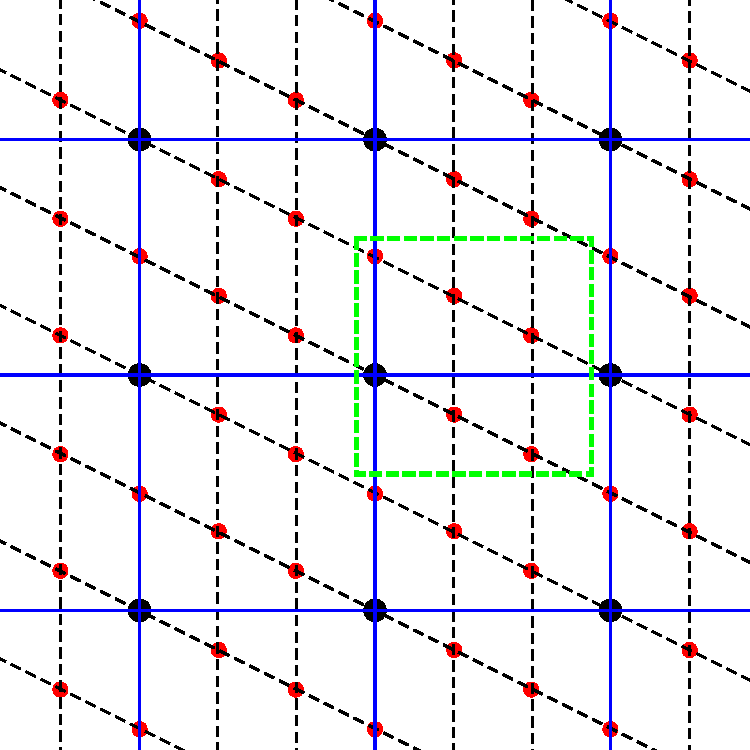
\includegraphics[width=0.40\textwidth]{HLReciprocalLattice2}
  \caption{\label{fig:HLReciprocalLattice2}
(Color online)
The reciprocal lattices of both the Bravais lattice $\lattice$ and the
integer square lattice. The red points are the reciprocal lattice $\lattice^*$ of the Bravais
lattice $\lattice$ in \reffig{fig:BravaisLatt}. The black points are
the reciprocal lattice of the square lattice. Each of these squares
enclosed by the blue lines has edge length $2 \pi$.
%And these squares are also repeating unit of the wave vectors (the red dots in this figure).
Two wave vectors are equivalent if they are different by a
reciprocal lattice vector of the square lattice.
}
\end{figure}
%%%%%%%%%%%%%%%%%%%%%%%%%%%%%%%%%%%%%%%%%%%%%%%%%%%%%%%%%%%%%%%



\subsection{Backup from s previous version of \catlatt}

The set of all wave vectors $\mathbf{K}_m$ that yield plane waves with
the periodicity of a given Bravais lattice defines its reciprocal
lattice. The $\mathbf{K}_m$ are called reciprocal lattice vectors.

% from Barvinok \arXiv{/math/0504444}:
Let $\langle \cdot, \cdot \rangle$ be the scalar product on $\reals^d$.
% and the corresponding Euclidean norm $\| \cdot\|$.
Let $\lattice \subset\reals^d$ be a lattice,
and let  $\lattice^{\ast} \subset\reals^d$ be its {\it reciprocal} lattice
\beq
\lattice^{\ast}=
\Bigl\{x \in \reals^d: \quad \langle x, y \rangle \in {\Bbb Z} \quad
\mbox{for all} \quad y \in \lattice
\Bigr\}\,.
\ee{dualLatt}

The reciprocal lattice of the Bravais lattice \refeq{2DBravaisLattice} is
spanned by reciprocal basis \refeq{RecLattBasis}
\beq
\lattice^* = \{n_1 \mathbf{b}_1 + n_2 \mathbf{b}_2\,|\,n_i \in \mathbb{Z}\}
\,.
\ee{2DReciprocalLattice}
The eigenvectors of the translation operator have the form
of a plane wave
\beq
f_{k}({z})
= e^{i {k} \cdot {z}} \, , \quad {k} \in \lattice^*
\,,
\ee{2DEigenvectors}
and, in addition, satisfy the Bravais lattice \refeq{2DBravaisLattice}
periodicity.



Then the basis vectors of the reciprocal lattice are:
\beq
\left[
\begin{array}{cc}
\mathbf{b}_1 & \mathbf{b}_2 \\
\end{array}
\right]
=
\frac{2 \pi}{\speriod{} \period{}}
\left[
\begin{array}{cc}
 \period{} & 0 \\
 -{S} & \speriod{} \\
\end{array}
\right]
 \, .
\ee{2DReciprocalBasis}
A plane wave with wave vector $\mathbf{k}$ in
the reciprocal lattice $\lattice^*$ is an eigenvector of the
{\jacobianOrb} \refeq{dDCatsT} that satisfies the periodic condition of
Bravais lattice $\lattice$. The eigenvector with wave vector
$\mathbf{k}=n_1\mathbf{b}_1+n_2\mathbf{b}_2$ is
\beq
f_{k}({z}) = e^{i {k} \cdot {z}}
  = \exp\left(
      i\frac{2 \pi}{\speriod{} \period{}}(n_1 \period{} z_1 - n_1 {S} z_2 + n_2 \speriod{} z_2)
        \right)
\,,
\ee{2DEigenvector}
where the ${z}=(z_1,z_2)$, with the {\jacobianOrb}  eigenvalue
\beq
\lambda_{k}
= \sum_{j=1}^2 ({s} - 2 \cos k_j)
= 2s - 2 \cos2\pi(\frac{n_1}{\speriod{}})
    - 2 \cos2\pi(\frac{n_1 {S}}{\speriod{} \period{}}
                -\frac{n_2}{\period{}})
\,.
\ee{2DEigenvalue}
As the field has support on the square lattice sites, it suffices to use
the wave vectors
$\mathbf{k}= n_1 \mathbf{b}_1 + n_2 \mathbf{b}_2$
with $n_1$ from 0 to $\speriod{}-1$ and $n_2$ from 0 to $\period{}-1$ to
get all the reciprocal lattice eigenvectors.
    \PC{2020-05-28}{Perhaps use
\[
\cos(a-b) = \cos(a)\cos(b) + \sin(a)\sin(b)
\,?
\]
\[
\cos(2a) = \cos(a)^2 - \sin(a)^2 = 1 - 2\sin(a)^2
\,?
\]
\[
{s}-2\cos k_1  = ({s}-2) + 4(\sin(k_1/2))^2
\]
\[
{s}-2\cos k_2  = ({s}-2) + 4(\sin(k_1/2))^2
\]
Set \(q_1=2\pi{k_1}/{\speriod{}}\,,\)
\(q_2=2\pi{k_2}/{\period{}}\,,\)
\(C=\speriod{}/{\period{}}\,,\)
\[
2\cos(q_2-Cq_1) = 2\cos(q_2)\cos(Cq_1) + 2\sin(q_2)\sin(Cq_1)
\]
or
\[
\lambda_m = 2-2\cos\alpha_m = 4 \sin^2\left(\alpha_m/2\right)
\,,\quad
\alpha_m=\pi{m}/{n}
\] %\ee{Pozrikidis14(1.2.7)}
we should state the
$\sin^2\left(\alpha_m/2\right)$ version of the eigenvalues
at least once.
    }

This range contains all of the wave vectors in one lattice cell of
reciprocal lattice of the square lattice, as shown in
\reffig{fig:HLReciprocalLattice2}, where wave vectors with $n_1$ from 0
to $\speriod{}-1$, and $n_2$ from 0 to $\period{}-1$ are enclosed by the
green dashed square. Any wave vector on the reciprocal lattice
$\lattice^*$ outside of this range will give an eigenvector which is
equivalent to an eigenvector with the wave vector within this range. So
the number of eigenvectors is $\speriod{} \period{}$, which is the number
of square lattice sites within the minimal repeating tile.

The 4-index {\jacobianOrb} \refeq{dDCatsT} is a matrix with indices in a
finite range. The {\jacobianOrb} has $\speriod{}\period{}$ eigenmodes. We
know that the number of {\twots} is equal to the {\HillDet} of the
{\jacobianOrb}, which is the product of all the eigenvalues,
% $N_{\LTS{}{}{}}=\prod_{k}\lambda_{k}$,
\beq
N_{\LTS{}{}{}}
=  2^{\speriod{}\period{}}\prod_{k_1=0}^{\speriod{}-1} \prod_{k_2=0}^{\period{}-1}
     \left[s  -  \cos\left(\frac{2\pi k_1}{\speriod{}}\right)
              -  \cos\left(
                            \frac{2\pi k_2}{\period{}}
                           -\frac{2\pi k_1}{\speriod{}}
                            \frac{ \tilt{}}{\period{}}
                     \right)
     \right]
%.
\label{2DCountingFormula}
\eeq

Given the eigenmodes with a given periodic condition, one can reduce the
2\dmn\ square lattice to a finite repeating tile. The {\sPe} in this tile
is still \refeq{dDCatsT}. But now the fields and sources are defined over an
$\LTS{}{}{}$ lattice.

\beq
N_{\BravCell{1}{1}{0}} =  2s - 4 = 1
 \,.
\label{1x1DCount}
\eeq

\beq
N_{\BravCell{\speriod{}}{1}{0}}
=  \prod_{k_1=0}^{\speriod{}-1}
     \left[2s_2 - 2 - 2 \cos\left(\frac{2\pi k_1}{\speriod{}}\right)
     \right]
 \,.
\label{2Dto1DCount}
\eeq
Comparing with the \templatt\ count \refeq{appe:detTemCatCheb} we see
that the count is the same, provided we replace
\(
{s}_1\to2({s}_2-1)
\,,
\)
in agreement with the 3-term recurrence \refeq{eq:CatLattT=1}.


\subsubsection{$\BravCell{2}{1}{1}$ \twots.}
\label{s:catLatt2x2rel1}
%    \HLpost{2019-11-22}{
For $s=5/2$ \catlatt.
\beq
N_{\BravCell{2}{1}{1}}
= \prod_{l=0}^{1}
  \Big[
  2s - 4 \cos2\pi\left(\frac{l}{2}\right)
  \Big]
= 9
 \,.
\ee{2x1_1Fourier}

\subsubsection{$\BravCell{2}{2}{0}$ \twots.}
\label{s:catLatt2x2}
For $s=5/2$ \catlatt.
\[
N_{[2\!\times\!2]} =
2^4({s}- 2)({s}- \cos\pi -1)({s}- 1 - \cos\pi)({s}- \cos\pi - \cos\pi) = 225
\,.
\]

\subsubsection{$\BravCell{3}{2}{0}$ \twots.}
\label{s:catLattRel3x2}
%    \HLpost{2019-11-23}{
For $s=5/2$ only 850 prime $\BravCell{3}{2}{0}$ \brick s are \admissible. The
integer points count \refeq{HL[3x2]count} is in agreement with the
counting formula \refeq{2DCountingFormula} for the $\BravCell{3}{2}{0}$
\twots:
     \[
N_{\BravCell{3}{2}{0}}
  = \prod_{l=0}^2\prod_{t=0}^1\left[
  2{s}-2\cos\left(\frac{2 \pi l}{3}\right)-2\cos\left(\frac{2 \pi t}{2}\right)
                              \right]
  = 5120
     \,.
     \]

%%%%%%%%%%%%%%%%%%%%%%%%%%%%%%%%%%%%%%%%%%%%%%%%%%%%%%%%%%%%%%%%%%%%%%%
\renewcommand{\statesp}{phase space}
\renewcommand{\Statesp}{Phase space}
\renewcommand{\stateDsp}{phase-space}
\renewcommand{\StateDsp}{Phase-space}

    \ifboyscout\clearpage\fi
% siminos/kittens/catHamilton.tex                   pdflatex CL18
% $Author: predrag $ $Date: 2020-12-19 00:52:16 -0500 (Sat, 19 Dec 2020) $

\section{\AW\ partition of the cat map \statesp}
\label{s:catMapHam}

    \PC{2020-12-17}{
Remove from here, relink, once incorporated in ChaosBook.
    }
As explained in the companion paper\rf{GHJSC16},
the deep problem with the \PV\ code prescription is that it does not
yield a generating partition; the borders (\ie, $\ssp_0$, $\ssp_1$ axes)
of their unit-square partition
$(\ssp_{\zeit-1},\ssp_{\zeit})\in(0,1]\times(0,1]$
do not map onto themselves, resulting in the infinity of, to us unknown,
grammar rules for {\inadmissible} symbol sequences.

This problem was resolved in 1967 by Adler and
Weiss\rf{AdWei67,ArnAve,AdWei70} who utilized the stable/\-unstable
manifolds of the fixed point at the origin to cover a unit area torus by
a two-rectangles generating partition; for the \PV\ cat map
\refeq{eq:StateSpCatMap}, such partition\rf{DasBuch} is drawn in
 reffig{fig:PVAdlerWeiss}. Following Bowen\rf{Bowen70}, one refers to
such parallelograms as `rectangles'; for details
see Devaney\rf{deva87}, Robinson\rf{Robinson12}, or
ChaosBook\rf{DasBuch}. Siemaszko and Wojtkowski\rf{SieWoj11} refer to
such partitions as the `Berg partitions', and Creagh\rf{Creagh94} studies
their generalization to weakly nonlinear mappings.

While Percival and Vivaldi were well aware of \AW\ partitions, they felt
that their ``coding is less efficient in requiring more symbols, but it
has the advantage of linearity.'' Our construction demonstrates that one
can have both:  an \AW\ generating cat map partition, and a linear code.
The only difference from the \PV\ formulation\rf{PerViv} is that one
trades the single unit-square cover of the torus of
\refeq{eq:StateSpCatMap} for the dynamically intrinsic, two-rectangles
cover, but the effect is magic - now every
infinite walk on the {\markGraph}
corresponds to a unique {\admissible} orbit $\{\ssp_{\zeit}\}$, and the
{\markGraph} generates all {\admissible} itineraries $\{\Ssym{\zeit}\}$.

To summarize:
an explicit \AW\ generating partition completely solves the Hamiltonian cat map
problem, in the sense that it generates all {\admissible} orbits.
Rational and irrational initial states generate periodic and ergodic
orbits, respectively\rf{PerViv87b,Keating91}, with every \statesp\ orbit
uniquely labeled by an {\admissible} bi-infinite itinerary of symbols
from alphabet \A.

    \PC{2020-02-08}{
Note:
$N_2=\Det\jMorb=({s}-2)({s}+2)$,
$N_3 %   = {s}^3-3{s}-2
    = ({s}-2)({s}+1)^2$,
$N_4 = ({s}-2)({s}+1)\,{s}^2$,
$N_5 = ({s}-2)(s^2+ s-1 )^2$.
I think the factorization is true for all $\cl{}$, as the $s=2$ Laplacian
has a zero mode (constant $\ssp_i$, I think).

an sequence of non-negative integers counting the orbits of
a map; the sequence of periodic points for that map.
    }

This derivation was based on the \AW\ generating partition, a clever
explicit visualization of the cat map dynamics, whose generalization to
several coupled maps (let alone spatially infinite coupled cat
maps lattice) is far from obvious: one would have to construct covers of
high-dimensional {\fundPip}s by sets of sub-volumes.
However, as Keating\rf{Keating91} explains, no such explicit generating
partition is needed to count cat map \po s.

    \ifboyscout\clearpage\fi
% siminos/kittens/stab.tex  % called by CL18.tex
% $Author: predrag $ $Date: 2020-12-23 14:59:59 -0500 (Wed, 23 Dec 2020) $

\section{\Spt\ stability}
\label{s:stab}
% was siminos/spatiotemp/stability.tex  % called by blogCats.tex

\renewcommand{\deltaX}{\ensuremath{{\Delta \ssp}}}       %trajectory displacement

Here we address two questions:
(i) how is the high-dimensional orbit \jacobianM\ $\jMorb$ related
to the temporal [$d\!\times\!d$] \jacobianM\ $\jMat$?
and
(ii) how does one evaluate the orbit \jacobianM\ $\jMorb$?

\subsection{Temporal lattice}
\label{s:TempLatt}
% excerpted from \Chapter{cycles}{28sep2019}{Fixed points, and how to get them}
%

    \PCedit{
\beq
\jMorb_\Mm  = \id-\jMat \otimes \hopMat^{-1}
\,,
\ee{dDmnForwardJacobianTMP}

the {temporal Bernoulli}
condition \refeq{tempBern} is the zero of function
\beq
F[\Xx;\Mm[ = \jMorb\Xx+\Mm = 0
\,,\qquad
\jMorb = \id-{s}{\hopMat}^{-1}
\,,
\ee{tempBern-TMP}
    }

For a $d$\dmn\ discrete time map $\map$, with the lattice state $\Xx$ of
discrete period $\cl{}$, every temporal lattice site satisfies
\beq
\ssp_{\zeit+1}=\map(\ssp_\zeit)
\,,
\ee{CyclePntErr}
where $\ssp_\zeit$ is a $d$\dmn\ field at lattice site $\zeit$.
Consider an approximate lattice state, known only to a finite precision
\beq
\hat{\Xx}=(\hat{\ssp}_1,\hat{\ssp}_2,\cdots,\hat{\ssp}_\cl{})
\,,\quad
\hat{\ssp}_\zeit = \ssp_\zeit+\deltaX_\zeit
\,,
\ee{nXdCycleErr}
where $\ssp_\zeit$ is the exact field at lattice site \zeit.
Define the error field by
$F[\hat{\Xx}]=\map(\hat{\Xx})-\hopMat^{-1}\otimes\hat{\Xx}$, an operator
which compares the forward map of every point in $\hat{\Xx}$ with the
next point $\hat{\Xx}\otimes\hopMat$.

$F[\hat{\Xx}]$ is a $(\cl{}\!\times\!d)$\dmn\ temporal
lattice field obtained by stacking a $d$\dmn\ field $\hat{\ssp}_\zeit$ at
each of the $\cl{}$ lattice sites,
\beq
 F[\hat{\Xx}] \, = \, F
\left (
\begin{array}{l}
 \hat{\ssp}_1 \\ \hat{\ssp}_2 \\ \cdots \\ \hat{\ssp}_\cl{}
\end{array}
\right )
=
\left (
\begin{array}{l}
  \hat{\ssp}_1 - \hat{\map}_\cl{} \\ \hat{\ssp}_2 - \hat{\map}_1 \\
  ~~~\cdots \\ \hat{\ssp}_\cl{} - \hat{\map}_{\cl{}-1}
\end{array}
\right )
\,,\qquad \hat{\map}_\zeit = \map(\hat{\ssp}_\zeit)
\,,
\ee{errorVecs1D}
which measures the misalignment of every finite forward-in-time segment
$\map(\hat{\ssp})_\zeit$ with the next site $\hat{\ssp}_{\zeit+1}$ on the
lattice state $\hat{\Xx}$.

By \refeq{CyclePntErr}, the exact lattice state $\Xx$
% \refeq{nXdCycle}
is a zero of this vector field, $F[\Xx]=0$. Assuming that the $d$\dmn\
error vectors $\deltaX_\zeit$ are small in magnitude, and Taylor expanding the
{one discrete time-step} map $\map$ to linear order around the exact
solution,
\[
\map(\ssp_\zeit + \deltaX_\zeit)
   = \ssp_{\zeit+1} + \jMat_\zeit \deltaX_\zeit
    + (\cdots)
%\,,\qquad \map_\zeit = \map(\ssp_\zeit) = \ssp_{\zeit+1}
\,,
\]
where
\beq
[\jMat_\zeit]_{ij} = \frac{\pde \map_i(\ssp_\zeit)}{\pde \ssp_j}
    \,,\quad
\zeit
    = (1,2,\cdots,\cl{})
    \,,\quad
i,j
    \,=\, (1,2,\cdots,d)
\label{Hill:FntTimeJac}
\eeq
one finds that the neigh\-bor\-hood of entire cycle $p$ is
linearly deformed by the $[\cl{}d\times\cl{}d]$ orbit \jacobianM\
\beq
    \deltaX' = \jMorb(\ssp) \, \deltaX
    \,, \qquad
\jMorb_{ij}(\ssp)
  =  \frac{\delta F[\ssp]_i}{\delta \ssp_j}
\,,
\ee{stab:hOdes}
with
\[
{\cal J} \,=\,
1 - \hopMat \jMat
\,,
\]
the one discrete time-step temporal [$d\!\times\!d$] \jacobianM\
$\jMat$ evaluated on the entire cycle $p$, and $\hopMat$ the {\shiftOp}
\beq
\hopMat
= \left(
\begin{array}{cccccc}
%=\begin{bmatrix}
             0    &       &        &        &   &  \id\cr
           \id  &  0    &        &        &   &  \cr
                  & \id &   0    &        &   &  \cr
                  &       & \id  &        &  &  \cr
                  &       &        &   \ddots & 0 &  \cr
                  &       &        &        & \id & 0
%        \end{bmatrix}
\end{array}
\right)
\,,\quad
\jMat
= \left(
\begin{array}{cccccc}
%=\begin{bmatrix}
          \jMat_1 &      &        &        &   &  \cr
                  & \jMat_2 &    &        &   &  \cr
                  &       &\jMat_3 &      &   &  \cr
                  &       &        & \ddots & &  \cr
                  &       &        & & \jMat_{\cl{}-1} &  \cr
                  &       &        &      &   & \jMat_{\cl{}}
%         \end{bmatrix}
\end{array}
\right)
\,,
\ee{shiftMatrix}
with $\id$ in the upper right corner assuring periodicity,
$\hopMat^\cl{}=\id$.

Consider a $d$-\dmn\ map $\ssp_{\zeit+1}=\map(\ssp_{\zeit})$, where
$\ssp_{\zeit}=\{\ssp_{\zeit,1},\ssp_{\zeit,2},\dots,\ssp_{\zeit,d}\}$ is
the state of the system at time $\zeit$. In case at hand, the one time step \jacobianM\
\beq
\jMat(\ssp_{\zeit})_{ij}
=
\left.\frac{\partial \map(\ssp)_i}{\partial \ssp_{j}}\right|_{\ssp_{i}=\ssp_{i,\zeit}}
%\,.
\ee{dDmn1stepJac}
stretches uniformly, so the \jacobianM\ does not depend on
the field value $\ssp_{\zeit}$ or time $\zeit$, $\jMat(\ssp_{\zeit}) =
\jMat$.

For a lattice state $\Xx_p$ with period $\cl{}$, the \jacobianOrb\ is a
$[\cl{}d\times\cl{}d]$ block matrix
\beq
\begin{array}{cc}
 \\ \\ \jMorb & = \\ \\
\end{array}
\left(
\begin{array}{ccccc}
\id    & & & & -\jMat \\
-\jMat & \id & \\
& ~~\cdots~~    & \id \\
 & & ~~\cdots~~ & \id \\
 & & &-\jMat    & \id
\end{array}
\right)
= \id-\jMat \otimes \hopMat^{-1}
\,,
\ee{dDmnForwardJacobian}
where $\id$ is a $d$-\dmn\ identity matrix, $\jMat$ is the
one time step $[d\times d]$ \jacobianM\ \refeq{dDmn1stepJac},
and $\hopMat$ is the $[\cl{}\times\cl{}]$ {\shiftOp} matrix with period $\cl{}$.

To evaluate the {\HillDet} of the \jacobianOrb, expand $\ln \Det \jMorb_p = \Tr \ln \jMorb_p$:
\bea
\ln \Det \jMorb_p
&=& \Tr \ln (\id-\jMat \otimes \hopMat^{-1}) \continue
&=& - \sum_{k=1}^{\infty} \frac{\Tr (\jMat \otimes \hopMat^{-1})^k}{k}
\, .
\label{dDmnForwardJacobianLnDet}
\eea
Note that $(\jMat \otimes \hopMat^{-1})^k = \jMat^k \otimes \hopMat^{-k}$ and
$\Tr (\jMat^k \otimes \hopMat^{-k})
= \Tr (\jMat^{\cl{}r} \otimes \id_{[\cl{}\times\cl{}]}) \delta_{k,\cl{}r}
= \cl{} \tr (\jMat^{\cl{}r}) \delta_{k,\cl{}r}
$
 which is not 0 only when $k$ is a multiple of $\cl{}$.
\bea
\ln \Det \jMorb_p
&=& - \sum_{r=1}^{\infty} \frac{\cl{} \tr (\jMat^{r\cl{}})}{r\cl{}}
 =  \tr [- \sum_{r=1}^{\infty} \frac{(\jMat^{\cl{}})^r}{r}] \continue
&=& \tr \ln (\id - \jMat^{\cl{}})
 =  \ln \det (\id - \jMat^{\cl{}})
\, .
\label{dDmnForwardJacobianLnDet2}
\eea
So the {\HillDet} of the \jacobianOrb\ is $\Det \jMorb = \det (\id - \jMat^{\cl{p}})$.

\HL{2020-01-21}{
A possible problem is $\jMorb_p$ could be negative. And here we have the one time step
 \jacobianM\ instead of a scalar $s$ so I'm not sure if we can expand $\ln (\id-\jMat \otimes \hopMat^{-1})$
 as a series in $\jMat \otimes \hopMat^{-1}$...
}


%%%%%%%%%%%%%%%%%%%%%%%%%%%%%%%%%%%%%%%%%%%%%%%%%%%%%%%%%%%%%
\subsection{Temporal stability}

% ``Hill's formula''
To summarize, a discretized, temporal lattice \po\ linear stability can
be computed in two ways - either by computing the
$[\cl{}d\times\cl{}d]$ {\jacobianOrb} $jMorb$, or by computing $\jMat_p$
\beq
\Det \jMorb_\Mm = \det (1-\jMat_\Mm)
\,,
\ee{dissipHill}
where $\jMat_\Mm$ is the $\cl{}$ time-steps $[d\!\times\!d]$ forward-time
\jacobianM. In the limit of discretization $\cl{}\to\infty$ the left
hand side is a {\em functional} {\HillDet} of an $\infty$\dmn\ {\em
operator}. Nevertheless, thanks to the discrete Fourier diagonalization
of $\jMorb(x)$, \refappe{appe:Fourier}, the {\HillDet} $\Det \jMorb_\Mm$ is easier to compute
than the ill-posed $\jMat_\Mm$.
    \PC{2019-10-10}{
$\jMorb(x)$ is block-diagonalized by the discrete Fourier transform on a
periodic lattice of three sites.
Write up next the discrete Fourier evaluation of $\Det \jMorb_p$.
    }
    \PC{2019-10-10}{
Rewrite the derivation of the Hill-\Poincare-Van Vleck stability matrix
\refeq{HL2DJacobianUpperTriangular} for symplectic / Lagrangian {\jacobianOrb}
using the {\shiftOp} \refeq{tempStab3cyc:shift}.
    }

The projection operator on the $k$th Fourier mode is
\beq
P_k = \prod_{j\not= k}^{} \frac{\hopMat-\omega_j \id }
                           {\omega_k - \omega_j}
\,.
\ee{hToN-ProjOp}
The set of the projection operators is complete,
\beq
\sum_k P_k = \id
\,,
\label{compl-ProjOp}
\eeq
 and orthonormal
\beq
P_k P_j = \delta_{kj} P_k
 \qquad (\hbox{no sum on} \ k)
\label{orthon-ProjOp}
\,.
\eeq
[TO BE CONTINUED]


\section{\Spt\ lattice}
\label{s:SptLatt}

In \spt\ settings, $\jMat_p$ can be defined only for finite numbers of
spatial sites, and it gets funkier and funkier as the spatial direction
increases (that is why we are able to work only with very small spatial
domain \KS\ discretizations). But, as shown for the \catlatt\ in
\refref{CL18}, $\Det {\cal J}_p$ works just fine on any
\spt\ torus. In particular, for any \twot\ \KS\ discretization.

\PC{2020-05-31} {
Politi and Torcini\rf{PolTor92} numerical method for finding \twots\ of
\emph{\spt\ H{\'e}non} is an extension of Biham and Wenzel\rf{afind} for
a single H{\'e}non map. Any fixed point in Biham-Wenzel fictitious time
corresponds to a doubly-periodic \spt\ cycle
$\BravCell{\speriod{}}{\period{}}{\tilt{}}$.
    }


\renewcommand{\deltaX}{\ensuremath{{\delta \ssp}}}       %trajectory displacement

    \ifboyscout\clearpage\fi
% siminos/kittens/symbolic.tex  % called by blogCats.tex and CL18.tex
% $Author: predrag $ $Date: 2021-08-10 11:56:19 -0400 (Tue, 10 Aug 2021) $

\ifblog
\chapter{Symbolic dynamics: a glossary}
\label{s-SymbDynGloss}
\else % called by kittens/CL18.tex
\section{Symbolic dynamics: a glossary}
\label{s-SymbDynGloss}
\fi
%%%%%% ChaosBook convention start %%%%%%%%%%%%%%%%%%%%%
\renewcommand{\statesp}{state space}
\renewcommand{\Statesp}{State space}
\renewcommand{\stateDsp}{state-space}
\renewcommand{\StateDsp}{State-space}

Analysis of a low\dmn\ chaotic dynamical system typically
starts\rf{DasBuch} with establishing that a flow is locally stretching, globally
folding. The flow is then reduced to a discrete time return map by appropriate
Poincar\'e sections. Its state space is partitioned, the partitions labeled by an
alphabet, and the qualitatively distinct solutions classified by their temporal
symbol sequences. Thus our analysis of the cat map and the {\catlatt} requires
recalling and generalising a few standard symbolic dynamics notions.

%\noindent
{\bf Partitions, alphabets.}
A division of {\statesp} $\pS$ into a disjoint union of distinct regions
$\pS_A,\pS_B,\ldots,\pS_Z$ constitutes a {\em
partition}. Label each region by a symbol $\Ssym{}$ from an
$N$-letter  {\em alphabet}
$\A=\{A,B,C,\cdots,Z\}$, where $N=\cl{\A}$ is
the number of such regions. Alternatively, one can distinguish different
regions by coloring them, with colors serving as the ``letters'' of the
alphabet.
% missing in kittens:  , as in \reffigs{fig:SingleCatPartit}{fig:AKScloseActSp}.
For notational convenience, in alphabets we sometimes denote negative integer
$\Ssym{}$ by underlining it, as in
\(
\A = \{ -{2}, -{1}, 0, 1\}
   = \{ \underline{2}, \underline{1}, 0, 1\}
\,.
\)


%\noindent
{\bf Itineraries.}
For a dynamical system evolving in time,
every {\statesp} point $\xInit \in \pS$ has the {\em future itinerary},
an infinite sequence of symbols
$\Sfuture(\xInit)=\Ssym{1}\Ssym{2}\Ssym{3}\cdots$ which indicates the
temporal order in which the regions shall be visited. Given a trajectory
$\ssp_1,\ssp_2,\ssp_3,\cdots$ of the initial point $\xInit$ generated
by a time-evolution law
\( %beq
   \ssp_{n+1}=f(\ssp_n)
    % \,, \quad \ssp_0=\xInit
\,,
\) %ee{CMx-iterated}
the itinerary is given by the symbol sequence
\beq
   \Ssym{n} = \Ssym{} \qquad \mbox{if\ } \qquad  \ssp_n \in \pS_{\Ssym{}}
 \,.
\ee{CMsymbol-def}
The {\em past itinerary} $\Spast(\xInit)=\cdots\Ssym{-2}
\Ssym{-1}\Ssym{0} $ describes the order in which the regions were visited
up to arriving to the point $\xInit$. Each point $\xInit$ thus has
associated with it the bi-infinite itinerary
\beq
\Sbiinf(\xInit) % = (\Ssym{k})_{k\in \integers}
        = \Spast.\Sfuture  =
 \biinf{\Ssym{-2}\Ssym{-1}\Ssym{0}}{\Ssym{1}\Ssym{2} \Ssym{3}}
\,,
\ee{CMbiifs}
or simply `itinerary', if we chose not to use the decimal point
to indicate the present,
\beq
   \{\Ssym{\zeit}\} = \cdots\Ssym{-2}\Ssym{-1}\Ssym{0}\Ssym{1}\Ssym{2} \Ssym{3}\cdots
\ee{Itinerary}


%\noindent
{\bf Shifts.}
A forward iteration of temporal dynamics $x\rightarrow x' = f(x)$ shifts
the entire itinerary to the left through the `decimal point'. This
operation, denoted by the {\shiftOp} \shift{},
\beq
   \shift{}(\biinf{\Ssym{-2}\Ssym{-1}\Ssym{0}}{\Ssym{1}\Ssym{2} \Ssym{3}})
     =  \biinf{ \Ssym{-2}\Ssym{-1}\Ssym{0}\Ssym{1}}{ \Ssym{2} \Ssym{3}}
\,,
\ee{CMshift-s}
demotes the current partition label $\Ssym{1}$ from the future $\Sfuture$
to the past $\Spast$.
The inverse shift $\shift{}^{-1}$ shifts the entire itinerary one step
to the right.

The set of all itineraries that can be formed from the letters of the
alphabet $\A$ is called the {\em full shift}
\beq
% \A^\integers 2017-08-05 Predrag dropped this notation
\hat{\AdmItnr} = \{ (\Ssym{k})
              : \Ssym{k} \in \A \quad \mbox{for all} \quad k \in  \integers \}
\,.
\ee{CMFullSh}

The itinerary is infinite for any trapped (non-escaping or \nws\ orbit) orbit
(such as an orbit that stays on a chaotic
repeller), and infinitely repeating for a periodic orbit $p$ of period \cl{p}.
A map $f$ is said to be a \emph{horseshoe} if its restriction to the \nws\ is
hyperbolic and topologically conjugate to the full $\A$-shift.

%\noindent
{\bf Lattices.}
Consider a $d$\dmn\ hypercubic lattice infinite in extent, with each site
labeled by $d$ integers $z\in \integers^{d}$. Assign to each site $z$ a
letter \Ssym{z}\ from a finite alphabet $\A$. A particular fixed set
of letters  \Ssym{z}\ corresponds to a particular {\lattstate}
\(
\Mm= \{\Ssym{z}\} % \in \A \,,\; z\in \integers^d \}
\,.
\)
%infinite in extent along all directions.
In other words, a $d$\dmn\ lattice requires a {$d$\dmn\ code}
\(
% \{\m_{z}\}
\Mm = \{\m_{n_1 n_2 \cdots n_d}\}
%\,,
\)
for a complete specification of the corresponding state $\Xx$.
In the lattice case, the {\em full shift} is the set of all $d$\dmn\
symbol \brick s that can be formed from the letters of the alphabet $\A$
\beq
% \A^{\integers^d}   2017-08-05 Predrag dropped this notation
\hat{\AdmItnr} = \{ \{\Ssym{z}\} % (\Ssym{z}) %_{z\in\integers^d}
              : \Ssym{z} \in \A \quad \mbox{for all} \quad z \in  \integers^d\}
\,.
\ee{LatticeFullSh}

%\noindent
{\bf Commuting discrete translations.}
%{\bf .}
%%%%%%%%%%%%%%%%%%%%%%%%%%%%%%%%%%%%%%%%%%%%%%%%%%%%%%%%%%%%%%%%%%%%%%%%
%    \PC{2016-01-12} {
% in the spirit of \refRefs{PetCorBol07}:
For an autonomous dynamical system, the evolution law $f$ is of the same form for
all times. If $f$ is also of the same form at every lattice site, the group of
lattice translations (sometimes called multidimensional shifts), acting along
$j$th lattice direction by shift $\shift{j}$, is a spatial symmetry that commutes
with the temporal evolution. A temporal mapping $f$ that satisfies
$f\circ\shift{j}=\shift{j}\circ{f}$ along the $d\!-\!1$ spatial lattice directions
is said to be {\em shift invariant}, with the associated symmetry of dynamics
given by the $d$\dmn\ group of discrete {\spt} translations.

\bigskip

Assign to each site $z$ a
letter \Ssym{z}\ from the alphabet $\A$. A particular fixed set
of letters  \Ssym{z}\ corresponds to a particular lattice symbol array
\(
\Mm= \{\Ssym{z}\} % \in \A \,,\; z\in \integers^d \}
 = \{\Ssym{n_1 n_2 \cdots n_d}\}
\,,
\)
which yields a complete specification of the corresponding state $\Xx$.
In the lattice case, the {\em full shift} is the set of all $d$\dmn\
symbol arrays that can be formed from the letters of the alphabet $\A$

as in \refeq{LatticeFullSh}

A $d$\dmn\ {\spt} field
\(
\Xx=\{\ssp_{z}\}
\)
is determined by the corresponding {\em $d$\dmn} {\spt}
symbol array
\(
\Mm=\{\Ssym{z}\}
\,.
\)
Consider next a finite \brick\ of symbols $\Mm_{\R}\subset\Mm$,
over a finite rectangular $[\speriod{1}\!\times\!\speriod{2}\!\times\cdots\times\!\speriod{d}]$
lattice region $\R\subset \integers^d$.
In particular, let $\Mm_{p}$ over a finite rectangular
$[\speriod{1}\!\times\!\speriod{2}\!\times\cdots\times\!\speriod{d}]$ lattice region be the
$[\speriod{1}\!\times\!\speriod{2}\!\times\cdots\times\!\speriod{d}]$ $d$-periodic \brick\ of
\Mm\ whose repeats tile $\integers^d$.

%\noindent
{\bf {\Brick s}.} In the case of temporal dynamics, a finite itinerary
\\
$\Mm_{\R}={\Ssym{k+1}\Ssym{k+2}\cdots\Ssym{k+\speriod{}}}$ of symbols from
$\A$ is called a {\em \brick} of length $\speriod{}=\cl{\R}$. More generally, let
$\R\subset\integers^d$  be a
$[\speriod{1}\!\times\!\speriod{2}\!\times\!\cdots\speriod{d}]$ rectangular lattice region,
$\speriod{k}\geq1$,
whose lower left corner is the $n=(n_{1}n_{2}\cdots{n_{d}})$ lattice site
\beq
  \R = \R_{n}^{[\speriod{1}\!\times\!\speriod{2}\!\times\!\cdots\speriod{d}]}
  =\{(n_1+j_1,\cdots n_d+j_d) \mid 0\leq j_k\leq \speriod{k}-1\}
\,.
\ee{dDimRect}
The associated finite {\brick} of symbols $\Ssym{z}\in\A$ restricted to  \R,
\(
\Mm_{\R}=\{\Ssym{z}| z\in \R \} \subset \Mm
\)
is called the \brick\ $\Mm_{\R}$ of volume
$\cl{\R} = \speriod{1}\speriod{2}\cdots\speriod{d}$. For example, for a 2\dmn\ lattice
a
$\R = [3\!\times\!2]$ \brick\ is of form
\beq
\Mm_{\R}=\left[\begin{array}{c}
\Ssym{12}\ \Ssym{22}\ \Ssym{32}\\
\Ssym{11}\ \Ssym{21}\ \Ssym{31}
\end{array}\right]
\ee{3times2brick}
and volume (in this case, an area) equals $3\times 2 = 6$.
In our convention, the first index is `space', increasing from left to right,
and the second index is `time', increasing from bottom up.

%\noindent
{\bf Cylinder sets.}
While a particular {\admissible} infinite symbol array
\(
\Mm= \{\Ssym{z}\} % \in \A \,,\; z\in \integers^d \}
\)
defines a point $\Xx$ (a unique {\lattstate}) in the \statesp,
the \emph{cylinder set}
$\pS_{\Mm_{\R}}$,
% $ \pS_{\R}$,
corresponds to the totality  of
\statesp\ points $\Xx$ that share the same given finite {\brick} $\Mm_{\R}$
symbolic representation over the region \R. For example, in $d=1$ case
\beq
\pS_{\Mm_{\R}} =
    \{\cdots a_{-2} a_{-1}\,.\,
   \Ssym{1}\Ssym{2}\cdots \Ssym{\speriod{}}
   a_{\speriod{}+1}a_{\speriod{}+2}\cdots\}
\,,
\ee{finiteBlock}
with the symbols  $a_{j}$ outside of the {\brick}
$\Mm_{\R}=[\Ssym{1}\Ssym{2}\cdots \Ssym{\speriod{}}]$
unspecified.
\index{block!finite sequence}
\index{cylinder!set}

%\noindent
{\bf \Po s, \dtors.}
A {\statesp} point $\ssp_z\in\Xx$ is {\spt}ly
{\em periodic}, $\ssp_z=\ssp_{z+\speriod{}}$, if its spacetime orbit returns to it
after a finite lattice shift
\(
\speriod{}= (\speriod{1},\speriod{2},\cdots,\speriod{d})
\)
over region $\R$ defined in \refeq{dDimRect}.
The infinity of repeats of the corresponding {\brick} $\Mm_{\R}$ then tiles the lattice.
For a {\spt}ly {periodic} state $\Xx$, a {\em prime} {\brick}
$\Mm_{p}$ (or $p$) is a smallest such \brick\
\(
\speriod{p}= (\speriod{1},\speriod{2},\cdots,\speriod{d})
\)
that cannot itself be tiled by repeats of a shorter {\brick}.

The periodic tiling of the lattice by the infinitely many repeats of a prime
{\brick} is denoted by a bar: $\cycle{\Mm}_{p}$. We shall omit the bar whenever
it is clear from the context that the state is periodic.
    \PC{2019-01-19}{eliminate \prune{ \Ssym{-m+1}\cdots \Ssym{0}} and
    \rctngl{ \Ssym{-m+1}\cdots \Ssym{0}},
    notation in favor a single convention}
    \PC{2018-11-07}{
    Generalize to \dtors.
    }


In $d=1$ dimensions, a prime {\brick} is called an {\em \orbit} $p$, a
% {\em prime} cycle
single traversal of the orbit; its label is a {\brick} of $\cl{p}$ symbols that
cannot be written as a repeat of a shorter {\brick}.
Each {\em periodic point}
\(
      \ssp_{ \Ssym{1} \Ssym{2} \cdots \Ssym{\cl{p}}}
\)
is then labeled by the starting symbol $\Ssym{1}$, followed by
the next $(\cl{p}-1)$ steps of its future itinerary.
The set of periodic points $\pS_p$ that belong to a given periodic orbit
form a {\em cycle}
\beq
p =  \cycle{ \Ssym{1} \Ssym{2} \cdots \Ssym{\cl{p}}}
  = \{
      \ssp_{ \Ssym{1} \Ssym{2}\cdots \Ssym{\cl{p}}},
      \ssp_{ \Ssym{2} \cdots \Ssym{\cl{p}} \Ssym{1}},
    \cdots,
      \ssp_{ \Ssym{\cl{p}} \Ssym{1}\cdots \Ssym{\cl{p}-1}}
     \}
\,.
\ee{PeriodCyc}

More generally, a {\statesp} point is {\em {\spt}ly periodic} if
it belongs to an \dtor, \ie, its symbolic representation is a \brick\
over region $\R$ defined by \refeq{dDimRect},
\beq
  \Mm_{p} = \Mm_{\R}
  \,,\qquad
  \R = \R_{0}^{[\speriod{1}\!\times\!\speriod{2}\!\times\cdots\times\!\speriod{d}]}
\,,
\ee{dTorus}
that
tiles the {\lattstate}  $\Mm$ periodically, with period $\speriod{j}$ in the
$j$th lattice direction.


%\noindent
{\bf Generating partitions.}
A temporal partition is called {\em generating} if every bi-infinite itinerary
corresponds to a distinct point in {\statesp}.
In practice almost any
generating partition of interest is infinite.
Even when the dynamics assigns a unique infinite itinerary
$\biinf{\Ssym{-2}\Ssym{-1}\Ssym{0}}{\Ssym{1}\Ssym{2} \Ssym{3}}$ to each
distinct orbit, there generically exist full shift itineraries
\refeq{CMFullSh} which are not realized as orbits; such sequences are
called {\em \inadmissible}, and we say that the symbolic dynamics is {\em
pruned}.

%\noindent
{\bf Dynamical partitions.}
If the symbols outside of given temporal {\brick} $b$ remain unspecified, the
set of all {\admissible} {\brick s} of length $\cl{b}$ yield a dynamically
generated partition of the \statesp, $\pS = \cup_b \pS_b$.

%\noindent
{\bf Subshifts.}
A dynamical system $(\pS,f)$ given by a mapping $f : \pS \to \pS$
together with a {partition} $\A$ induces {\em topological dynamics}
$(\AdmItnr,\shift{})$, where the {\em subshift}
\beq
\AdmItnr = \{  (\Ssym{k})_{k\in \integers} \}
\,,
\ee{subshift}
is the set of all {\em \admissible} itineraries, and
$\shift{} \,:\, \AdmItnr \to \AdmItnr$
is the {\shiftOp} \refeq{CMshift-s}. The designation `subshift' comes
from the fact that $\AdmItnr$
% \subset \hat{\AdmItnr}$
% \A^\integers 2017-08-05 Predrag dropped this notation
is a subset of the full shift.

%%%%%%%%%%%%%%%%%%%%%%%%%%%%%%%%%%%%%%%%%%%%%%%%%%%%%%%%%%%%%%%%%%%%%%%%
%    \PC{2016-10-11} { inspired by {Ban} \etal\rf{BHLL11}
Let $\hat{\AdmItnr}$ be the full lattice shift  \refeq{CMFullSh}, \ie,
the set of all possible {\lattstate} $\Mm$ labelings by the alphabet
$\A$, and $\hat{\AdmItnr}(\Mm_{\R})$ is
the set of such {\brick s} over a region {\R}. The principal task
in developing the symbolic dynamics of a dynamical system is to determine
$\AdmItnr$, the set of all \emph{{\admissible}} itineraries/{\lattstate}s,
\ie, all states that can be realized by the given system.

%\noindent
{\bf Pruning, grammars, recoding.}
If certain states are {\inadmissible}, the alphabet must be supplemented by a
{\em grammar},
a set of pruning rules.
Suppose that
the grammar can be stated as a finite number of pruning rules, each
forbidding a {\brick} of finite size,
\beq
 {\cal G} = \left\{
        b_1, b_2, \cdots b_k
        \right\}
\,,
\ee{grammar}
where a {\em pruned {\brick}} $b$ is an array of symbols defined over a
finite $\R$ lattice region of size
$[\speriod{1}\!\times\!\speriod{2}\!\times\cdots\times\speriod{d}]$. In
this case we can construct a finite Markov partition by replacing finite
size \brick s of the original partition by letters of a new alphabet. In
the case of a 1\dmn, the temporal lattice, if the longest forbidden {\brick}
is of length $L+1$, we say that the symbolic dynamics is Markov, a shift
of finite type with {$L$-step memory}.

%\noindent
{\bf Subshifts of finite type.}
A {topological dynamical system} $(\AdmItnr,\shift{})$ for which all
{\admissible} states $\Mm$ are generated by recursive application
of the finite set of pruning rules \refeq{grammar}
%of the  finite transition matrix
%\beq
%\AdmItnr = \left\{ (\Ssym{k})_{k\in \integers}
%           \,:\,
%                 T_{\Ssym{k} \Ssym{k+1}} = 1
%        \quad \mbox{for all $k$} \right\}
%\ee{AdmItnr}
is called a subshift of {\em finite type}.

                                            \toCB % to kneading.tex
If a map can be topologically conjugated to a linear map, the symbolic
dynamics of the linear map offers a dramatically simplified description
of all {\admissible} solutions of the original flow, with the temporal
symbolic dynamics and the state space dynamics related by linear recoding
formulas. For example, if a map of an interval, such as a parabola, can
be conjugated to a piecewise linear map, the kneading theory\rf{MilThu88}
classifies \emph{all} of its {\admissible} orbits.

%%%%%% ChaosBook convention,  BORIS conventions start %%%%%%%%%%%%%%%%%%%%%
\renewcommand{\statesp}{phase space}
\renewcommand{\Statesp}{Phase space}
\renewcommand{\stateDsp}{phase-space}
\renewcommand{\StateDsp}{Phase-space}
%%%%%% BORIS convention end   %%%%%%%%%%%%%%%

%%%%%%%%%%%%%%%%%%%%%%%%%%%%%%%%%%%%%%%%%%%%%%%%
\ifblog
% siminos/spatiotemp/chapter/symbolicIns.tex  pdflatex blog; biber blog
% $Author: predrag $ $Date: 2021-06-12 01:01:43 -0400 (Sat, 12 Jun 2021) $

%Predrag            2016-12-20

\section{Symbolic dynamics, inserts}
\label{s-SymbDynDefs}
% from ChaosBoook  \Chapter{knead}{15feb2015}{Charting the state space}

{\bf 2019-01-19 Predrag} Merge everything here to \refchap{s-SymbDynGloss}
{\em Symbolic dynamics: a glossary} then \texttt{svn rm} this file.

{\bf 2017-08-05 Predrag}
Consult / harmonize with  ChaosBook.org Chapter~{\em Charting the state space} (source file knead.tex).



%%%%%%%%%%%%%%%%%%%%%%%%%%%%%%%%%%%%%%%%%%%%%%%%%%%%%%%%%%%%%%%
\bigskip

to Predrag: check that all this is in Chaos\-Book, then erase:

\bigskip


The set of all bi-infinite itineraries that can be formed from the
letters of the alphabet ${\cal A}$ is called the
{\em full shift} (or {\em topological Markov chain})
\index{shift!full}
\index{Markov!chain}\index{topological!Markov chain}
% before \ee{FullSh}

Here we refer to this set of all conceivable itineraries
as the {\em covering} symbolic dynamics.
\index{symbolic dynamics!covering}
\index{covering!symbolic dynamics}

Orbit that starts out as a finite {\brick} followed by infinite number of
repeats of another {\brick} $p = (\Ssym{1} \Ssym{2} \Ssym{3} \cdots
\Ssym{\period{}})$ is said to be {\em heteroclinic} to the cycle $p$. An
orbit that starts out as $p^{\infty}$ followed by a different finite
{\brick} followed by $(p')^{\infty}$ of another {\brick} $p'$ is said to be a
{\em heteroclinic connection} from cycle $p$ to cycle $p'$.
    \index{heteroclinic!connection}



Suppose that
the grammar can be stated as a finite number of pruning rules, each
forbidding a {\brick} of finite length,
\index{symbolic dynamics!coding}
\beq
 {\cal G} = \left\{
        b_1, b_2, \cdots b_k
        \right\}
\,,
\ee{grammar1}
where a {\em pruned {\brick}} $b$ is a sequence of symbols
$b=\blok{ \Ssym{1} \Ssym{2} \cdots \Ssym{\cl{b}}}$,
 $\Ssym{} \in {\cal A}$,
of finite length $\cl{b}$.
\index{block, pruning}
\index{pruning!block}
\index{shift!finite type}
\index{symbolic dynamics!recoding}
\index{recoding}


\noindent{\bf Subshifts of finite type.}
A {topological dynamical system} $(\Sigma,\sigma)$ for
which all {\admissible} itineraries are generated by a finite
transition matrix
\beq
\Sigma = \left\{ (\Ssym{k})_{k\in \integers} \,:\, T_{s_k s_{k+1}} = 1
        \quad \mbox{for all $k$} \right\}
\ee{AdmItnr}
is called a subshift of {\em finite type}.

\noindent{\bf Reflection symmetries.}
Symmetries of the cat map induce  invariance with respect to
corresponding symbol exchanges. Define $\bar{m}=s\!-\!m\!-\!2$ to be the
conjugate of symbol $m \in \A$. For example, the two exterior
alphabet \Ae\ symbols are conjugate to each other, as illustrated by
\refeq{eq:StateSpCatMap}.
\PC{2019-05-27}{fix this eq. reference; edit it away}
If ${b}=\Ssym{1} \Ssym{2} \dots \Ssym{\ell}$ is a
\brick, and  $\bar{{b}}=\bar{m}_1 \bar{m}_2 \dots
\bar{m}_\ell$ its conjugate, then by  reflection symmetry of the cat
map we have  $|\Pol_{{b}}|= |\Pol_{\bar{{b}}}|$. Similarly, if
$b^*=\Ssym{l}\Ssym{l-1}\dots \Ssym{1}$, the time reversal invariance implies
$|\Pol_{{b}}|=|\Pol_{{b}^*}|$.

There are many ways to skin a cat. For example, due to the space
reflection symmetry about $\ssp=1/2$ of the \PV\ cat map
\refeq{eq:StateSpCatMap}, it is natural (especially in studies of
deterministic diffusion on periodic
lattices\rf{ArtStr97,CBdiffusion,CBappendDiff}) to center  the \statesp\
unit interval\rf{PerViv} as $\ssp\in[-1/2,1/2)$. In this formulation the
\PV\  cat map has a 5-letter alphabet
$\A=\{\underline{2},\underline{1},0,1,2\}$, in which the spatial
reflection symmetry is explicit (the ``conjugate'' of a symbol $m \in \A$
is $\bar{m}= -\!m$).
% , with \statesp\ partitions and pruning rules taking a symmetric form.

%%%%%%%%%%%%%%%%%%%%%%%%%%
% \renewcommand{\cl}[1]{{\ensuremath{|#1|}}}  % the length of a periodic orbit, Ronnie
 %symbolicIns}
\printbibliography[heading=subbibintoc,title={References}]
\fi
%%%%%%%%%%%%%%%%%%%%%%%%%%%%%%%%%%%%%%%%%%%%%%%%


    \ifsubmission
\section*{References}
    % from ctan.org/tex-archive/biblio/bibtex/contrib/iopart-num/ :
\bibliographystyle{iopart-num}       % APS-like style for physics
\bibliography{../bibtex/siminos}
    \else
\printbibliography[
heading=bibintoc,
title={References}
				  ] %, type=online]  % if not using default "Bibliography"
    \fi

%%%%%%%%%% Submission: cut here  %%%%%%%%%%%%%%%%%%%%%%%%%%%

    \ifboyscout
%    \clearpage
%\input{censored}
%    \PCedit{ %2019-05-27
%\section{Hill's formula}
%\label{c-Hill}  % temporary, while being edited in spatiotemp/
%% siminos/spatiotemp/chapter/action.tex
% $Author: predrag $ $Date: 2021-12-24 01:25:20 -0500 (Fri, 24 Dec 2021) $

% \ifblog  Predrag 2021-06-12 gave up on this,
%          do not remember who calls it other than blogCats.tex
    \chapter{Hill's formula}
    \label{c-Hill}  % temporary, while being edited in spatiotemp/
%\renewcommand{\cl}[1]{{\ensuremath{n_{#1}}}}   % discrete length of a cycle, Predrag
\renewcommand{\shift}{\ensuremath{\ell}}

\section{An overview over ``Hill's formulas''}
\label{sect:Hill}
%\renewcommand{\cl}[1]{{\ensuremath{|#1|}}}  % the length of a periodic orbit, Ronnie
\renewcommand{\shift}{\ensuremath{d}}

\begin{quote}
A succinct  explanation of the Hill's formula:\\
If you evaluate stability of the 3-term recurrence \refeq{JiKoKr20(2)} on
a periodic lattice you get the {\jacobianOrb} $\jMorb$;
if you evaluate it by multiplying the `two-configuration representation'
matrix $\jMps$, you get the `time evolution' side of the Hill's formula.
\end{quote}

We should emphasize that, while discovered first in Lagrangian setting,
Hill's formulas are much more general, they
apply also to dissipative dynamical systems as well, see

CL18 \HREF{http://chaosbook.org/~predrag/papers/CL18.pdf\#subsection.1.5}
{sect.~1.5} {\em  Stability of an orbit vs.  its time-evolution stability}

CL18 \HREF{http://chaosbook.org/~predrag/papers/CL18.pdf\#appendix.C}
{appendix~C} {\em Spatiotemporal stability}


\refsect{LiTom17b:GenFctn} {\em Generating functions; action}
%\else  Predrag 2021-06-12 gave up on this,
%          do not remember who calls it other than blogCats.tex
%\subsection{Generating functions; action}
%\fi


\refsect{sect:HillLagr} {\em Hill's formula, Lagrangian setting}


\refsect{sect:catlattHill} {\em \catLatt\ Hill's formula}


\refsect{sect:catlattHillrel} {\em Hill's formula for \rpo s}


\refsect{sect:templattHillHan} {\em Han's \templatt\ Hill's formula}


\refsect{sect:catlattHillHan} {\em Han's  \catlatt\ Hill's formula}


\refsect{sect:catlattHillRelativeHan} {\em Han's relative-periodic Hill's formula}


\refsect{sect:HenonHillHan} {\em Han's  \HenonMap\ Hill's formula}











\section{Generating functions; action}
%\else  Predrag 2021-06-12 gave up on this,
%          do not remember who calls it other than blogCats.tex
%\subsection{Generating functions; action}
%\fi
\label{LiTom17b:GenFctn}

    \PC{2016-11-11, 2018-09-26}{
What follows is (initially)
copied from Li and Tomsovic\rf{LiTom17b}, \emph{Exact relations between
homoclinic and \po\ actions in chaotic systems} arXiv source
file, then merged with the MacKay-Meiss-Percival action
principle \refrefs{MKMP84,meiss92}.
    }
For discrete-time one-degree-of-freedom Lagrangian systems satisfying a
periodicity condition (\ie, cat map):
\beq
\genF(\coord+1, \coord'+1)=\genF(\coord, \coord')+C
\,,
\ee{MacMei83-2}
one can consider relative periodic paths (or pre-periodic paths, also called
periodic paths of type $(\shift,\cl{})$ by Mackay and Meiss\rf{MacMei83}), with
    \PC{2018-09-29} {presumably they are \rpo s, or pre-\po s, with a rational
    winding number $p/\coord$.}
\beq
\coord_{i+\cl{}}=\coord_{i}+\shift
\,.
\ee{MacMei83-3}
Every $\coord_{i}$ returns to its value after time period $\cl{}$, but shifted by
$\shift$.
Orbits satisfying \refeq{MacMei83-3} are given by stationary points of the action
\beq
\action = \sum_{i=0}^{q-1} \genF(\coord_i, \coord_{i+1})
\ee{MacMei83-4}
in the space of periodic paths of type $(\shift,\cl{})$.
For periodic paths, it suffices to consider one period, because an orbit is periodic if
and only if it is a stationary point of the action of one period in the space
of periodic paths.

If the constant $C$ (the
\HREF{https://floerhomology.wordpress.com/2015/09/14/mean-action-and-the-calabi-invariant/}
{Calabi invariant}\rf{Calabi70}) in the periodicity condition
\refeq{MacMei83-2} is zero, and the Lagrangian satisfies a convexity
condition
\beq
\genF_{12}(\coord, \coord') < 0
\,,
\ee{MacMei83-5}
where subscript $k$ refers to the derivative with respect to the $k$th
argument, then the action of periodic paths of type  $(\shift,\cl{})$ is bounded below,
so there is a minimising path. Since its action is stationary, it gives a \po\
of type  $(\shift,\cl{})$.

    \PC{2018-01-21}{Is this true?
To go from the Hamiltonian $(\ssp_{\zeit},p_{\zeit})$ phase space formulation to the
Newtonian (or Lagrangian) $(\ssp_{\zeit-1},\ssp_{\zeit})$ {\em state space}
formulation, replace $p_\zeit$  by
\(
p_\zeit = (\ssp_{\zeit} - \ssp_{\zeit-1})/\Delta\zeit \,,
\)
where $\Delta\zeit =1$.
    }
    %
For {\orbit} ${p}$  of period $\cl{p}$, the {action} of the \orbit\ is:
\beq
\label{eq:DefGenFprimePOs}
\action_{p}  \equiv \sum_{n=0}^{\cl{p}-1}\genF(\coord_{n},\coord_{n+1})\ .
\eeq
$\action_{p}$ is the generating function that maps a point along the orbit for one
(prime) period.  For the case of a fixed point $p$ of period $\cl{p}=1$,
the action is
\beq\label{eq:Definition generating function fixed points}
\action_{p}  = \genF(\coord_p,\coord_p)
\,,
\eeq
where the generating function $\genF(\coord_p,\coord_p)$ maps $\ssp_p$ into itself in one
iteration.

\section{Homoclinic and \po\ actions in chaotic systems}

    \PC{2018-09-29}{
What follows is copied from Li and Tomsovic\rf{LiTom17b}.
    }
For an aperiodic orbit $\lbrace\ssp_0\rbrace$ going through the point $\ssp_0$,
the action, evaluated as the sum over an infinity of successive mappings,
\begin{equation}
\label{eq:full orbit action in general}
\action_{\lbrace \ssp_0 \rbrace}
\equiv \lim_{N \to \infty}
\sum_{n=-N}^{N-1} \genF(\coord_{n},\coord_{n+1})
=\lim_{N \to \infty} \action_{-N,N}
\,,
\end{equation}
is not necessarily convergent. However, the MacKay-Meiss-Percival action
principle\rf{MKMP84,meiss92} can be applied to obtain well defined
action differences between pairs of orbits.  For example,
the {\em relative} {\em action}
$\Delta \action_{\lbrace h_0 \rbrace  \lbrace x \rbrace}$ between a fixed point $\ssp_p$
and its homoclinic orbit $\lbrace h_{0} \rbrace$, where $h_{\pm
\infty}\to \ssp_p$:
\begin{eqnarray}
\label{eq:relative action homoclinic}
\Delta \action_{\lbrace h_0 \rbrace  \lbrace \ssp_p \rbrace}
 &\equiv & \lim_{N \to \infty} \sum_{i=-N}^{N-1}\left[\genF(h_i,h_{i+1})-\genF(\ssp_p,\ssp_p)\right]
\nonumber \\
&=& \int\limits_{U[\ssp_p,h_{0}]}p\mathrm{d}\coord+\int\limits_{S[h_{0},\ssp_p]}p\mathrm{d}\coord
= \oint_{US[\ssp_p,h_{0}]} p\mathrm{d}\coord \nonumber \\
&=& {\cal A}^\circ_{US[\ssp_p,h_{0}]}
\end{eqnarray}
where $U[\ssp_p,h_{0}]$ is the segment of the unstable manifold from $\ssp_p$ to
$h_{0}$, and $S[h_{0},\ssp_p]$ the segment of the stable manifold from $h_0$
to $\ssp_p$.  The $\circ$ superscript on the last line indicates that the area
is interior to a path that forms a closed loop, and the subscript
indicates the path: $US[\ssp_p,h_{0}]=U[\ssp_p,h_{0}]+S[h_{0},\ssp_p]$.  The
clockwise enclosure of an area is positive, counterclockwise negative.
$\Delta \action_{\lbrace h_0 \rbrace \lbrace \ssp_p \rbrace} $ gives the
action difference between the homoclinic orbit segment $[
h_{-N},\cdots,h_{N} ]$ and the length-$(2N+1)$ fixed point orbit segment
$[ \ssp_p, \cdots, \ssp_p ]$ in the limit $N \to \infty$. In later sections, upon
specifying the symbolic code of the homoclinic orbit $\lbrace h_0 \rbrace
\Rightarrow \overline{0} \gamma \overline{0}$, we also denote $\Delta
\action_{\lbrace h_0 \rbrace  \lbrace \ssp_p \rbrace}$ alternatively as
\begin{equation}\label{eq:relative action homoclinic symbolic notation}
\Delta \action_{\lbrace h_0 \rbrace  \lbrace \ssp_p \rbrace}
= \Delta \action_{\overline{0} \gamma \overline{0},  \overline{0}}
\end{equation}
by replacing the orbits in the subscript with their symbolic codes.

%%%%%%%%%%%%%%%%%%%%%%%%%%%%%%%%%%%%%%%%%%%%%%%%%%%%%%%%%%%%%%%%%%%%%
\begin{figure}
   
\includegraphics[width=0.5\textwidth]{LiTom17bHorseshoe2}
\caption{\label{fig:Horseshoe2}
A sketch of a partial homoclinic tangle
which forms a complete horseshoe structure. The unstable (stable)
manifold of $x$ is the solid (dashed) curve. There are two primary
homoclinic orbits $\lbrace h_0\rbrace$ and $\lbrace g_0\rbrace$.
$\cal{R}$ is the closed region bounded by loop
$\mathcal{L}_{USUS[x,g_{-1},h_0,g_0]}$.
~(From \refref{LiTom17b})
        }
\end{figure}
%%%%%%%%%%%%%%%%%%%%%%%%%%%%%%%%%%%%%%%%%%%%%%%%%%%%%%%%%%%%%%%%%%%%%

Likewise, a second important case is for the relative action between a
pair of homoclinic orbits $\lbrace h^{\prime}_0\rbrace \Rightarrow
\overline{0} \gamma^{\prime} \overline{0} $ and $\lbrace h_0\rbrace
\Rightarrow \overline{0} \gamma \overline{0}$, which results in
\begin{eqnarray}
\label{eq:homoclinic action difference}
\Delta \action_{{\lbrace h^{\prime}_0\rbrace}{\lbrace h_0\rbrace}} &\equiv & \lim_{N \to \infty} \sum_{i=-N}^{N-1}\left[ \genF(h^{\prime}_{i},h^{\prime}_{i+1}) - \genF(h_{i},h_{i+1})\right] \nonumber \\
& = & \lim_{N \to \infty} \left[ \genF(h^{\prime}_{-N},h^{\prime}_{N}) - \genF(h_{-N},h_{N}) \right] \nonumber \\
& = & \int\limits_{U[h_{0},h^\prime_{0}]}p\mathrm{d}\coord+\int\limits_{S[h^\prime_{0},h_{0}]}p\mathrm{d}\coord =  {\cal A}^\circ_{US[h_0,h^\prime_{0}]} \nonumber \\
& = & \Delta \action_{ \overline{0} \gamma^{\prime} \overline{0},  \overline{0} \gamma \overline{0} }
\end{eqnarray}
where $U[h_{0},h^\prime_{0}]$ is the segment of the unstable manifold
from $h_{0}$ to $h^\prime_{0}$, and $S[h^\prime_{0},h_{0}]$ the segment
of the stable manifold from $h^\prime_{0}$ to $h_{0}$.  Due to the fact
that the endpoints approach $\ssp_p$ forward and backward in time, one can
also write
\begin{eqnarray}
\label{eq:homoclinic action difference2}
\Delta \action_{{\lbrace h^{\prime}_0\rbrace}{\lbrace h_0\rbrace}}
& = & \lim_{N \to \infty}
\left[ \genF(h^{\prime}_{-(N+n)},h^{\prime}_{N+m}) - \genF(h_{-N},h_{N})
      \right] \nonumber \\
& & - (n+m) {\cal F}_0
\,.
\end{eqnarray}

%%%%%%%%%%%%%%%%%%%%%%%%%%%%%%%%%%%%%%%%%%%%%%%%
    \ifblog
\newpage
% siminos/kittens/Hill.tex      pdflatex CL18
% $Author: predrag $ $Date: 2020-12-23 14:59:59 -0500 (Wed, 23 Dec 2020) $

\section{{\HillDet}:
            stability of an orbit vs. its time-evolution stability}
\label{s:Hill}

The $d=2$ lattice \catlatt\ equations can be recast in a matrix form, by
rewriting the defining equations in terms of \emph{block
matrices}\rf{Dorr70,BuGoNi70,ChenM87,HuRyCo98}, constructed by the
\HREF{https://en.wikipedia.org/wiki/Kronecker_product} {Kronecker
product} $\mathbf{A}\otimes\mathbf{B}$, an operation
(introduced by Zehfuss in 1858) that replaces the $a_{ij}$
element of an [$n\times{n}$] matrix $\mathbf{A}$ by [$m\times{m}$]
matrix block $a_{ij}\mathbf{B}$, resulting in an [$mn\times mn$] block
matrix\rf{ArWeHa13,wikiKronProd}
\beq
\mathbf{A}\otimes\mathbf{B} =
\left[\begin{array}{ccc} %\begin{bmatrix}
  a_{11} \mathbf{B} & \cdots & a_{1n}\mathbf{B} \\
             \vdots & \ddots &           \vdots \\
  a_{n1} \mathbf{B} & \cdots & a_{nn} \mathbf{B}
\end{array}\right] %\end{bmatrix}
\,.
\ee{KronProd}
Consider $\mathbf{A}$, $\mathbf{A'}$ square matrices of size
[$n\times{n}$], and $\mathbf{B}$, $\mathbf{B'}$ square matrices of size
[$m\times{m}$].
The matrix product of two block matrices is a block
matrix\rf{ArWeHa13,wikiBlockMat},
\beq
(\mathbf{A}\otimes\mathbf{B})\,(\mathbf{A'}\otimes\mathbf{B'})
%= (\mathbf{A}\mathbf{A'})\otimes(\mathbf{B}\mathbf{D})
%  {\displaystyle (\mathbf {A} \otimes \mathbf {B} )(\mathbf {C} \otimes \mathbf {D} )
  =(\mathbf{AA'})\otimes (\mathbf{BB'})
  \,.
\ee{mixedProd}
The trace and the determinant of a block matrix are given by
\bea
\tr(\mathbf {A} \otimes \mathbf {B})
    &=& \tr\mathbf{A}\,\tr\mathbf{B}
    \continue
\det\left(\mathbf{A} \otimes \mathbf{B}\right)
    &=& \det\left(\mathbf{A}^{m}\right) \det\left(\mathbf{B}^{n}\right)
\,.
\label{wikiKron2}
\eea
The two [$mn\times mn$] block matrices $\mathbf{A}\otimes\mathbf{B}$ and
$\mathbf{B}\otimes\mathbf{A}$ are equivalent by a similarity
transformation
\beq
\mathbf {B} \otimes \mathbf {A}
=\transp{\mathbf {P}} \,(\mathbf {A} \otimes \mathbf {B} )\,\mathbf {P}
\,,
\ee{wikiKron3}
where $\mathbf{P}$ is permutation matrix. As $\det{\mathbf{P}}=1$,
the block matrix determinant
$\det\left(\mathbf{A}\otimes\mathbf{B}\right)
=
\det\left(\mathbf{B}\otimes\mathbf{A}\right)$
is independent of the order in which blocks are constructed.

Consider a rectangular $d=2$ lattice
$\BravCell{\speriod{}}{\period{}}{0}$ Bravais cell. The \jacobianOrb\
\refeq{catLatt} written as a
$[\speriod{}\period{}\times\speriod{}\period{}]$ Kronecker product block
matrix is
\beq
\jMorb
=
\id_{1} \otimes \left(\hopMat_{2}+\hopMat_{2}^{-1}\right)
-
2 {s}\,\id_1\otimes\id_{2}
+
\left(\hopMat_{1}+\hopMat_{1}^{-1}\right) \otimes \id_{2}
\,,
\ee{catalattLxT}
where the \refeq{KronProd} matrix $\mathbf{A}$ and identity
$\id_1$ matrix are `spatial' [$\speriod{}\!\times\!\speriod{}$]
matrices, with blocks $\mathbf{B}$ and identity $\id_2$ `temporal'
[$\period{}\!\times\!\period{}$] matrix blocks. Indices `1', `2'
referring to `spatial', `temporal' lattice directions, respectively.

Our task is to compute the {\HillDet} $|\det \jMorb|$. We first show how
to do that directly, by computing the volume of the {\fundPip}.

\subsection{{\HillDet}: fundamental parallelepiped evaluation}
\label{s:catLattRel3x2}
% 2020-02-16 Predrag computed  using siminos/mathematica/Tensors.nb
As a concrete example
consider the Bravais lattice \refeq{2DBravaisLattice} with basis
vectors $\mathbf{a}_1=(3,0)$ and $\mathbf{a}_2=(0,2)$. A \twot\ over this
Bravais cell has 6 field values, one for each lattice site $z=(n,\zeit)$
on a $\BravCell{3}{2}{0}$ rectangle:
\[
 \left[\begin{array}{ccc}
 \ssp_{01} & \ssp_{11} & \ssp_{21} \\
 \ssp_{00} & \ssp_{10} & \ssp_{20}
 \end{array}\right]
\,.
\]
Stack up the columns of this lattice state and the corresponding sources
into 6\dmn\ vectors,
\beq
\Xx_{\BravCell{3}{2}{0}} =
\left(\begin{array}{c}
 \ssp_{01} \\
 \ssp_{00} \\
  \hline
 \ssp_{11} \\
 \ssp_{10} \\
  \hline
 \ssp_{21} \\
 \ssp_{20} \\
      \end{array}\right)
\,,\qquad
\Mm_{\BravCell{3}{2}{0}} =
\left(\begin{array}{c}
 \Ssym{01} \\
 \Ssym{00} \\
  \hline
 \Ssym{11} \\
 \Ssym{10} \\
  \hline
 \Ssym{21} \\
 \Ssym{20} \\
        \end{array}\right)
\,.
\ee{3times2blockVect}
The corresponding {\jacobianOrb} \refeq{catlattFix}
%\([\BravCell{3}{2}{}\times \BravCell{3}{2}{}]\)
%4-index matrix $\jMorb_{zz'}$.
is the  block-matrix
\refeq{catalattLxT},
a block circulant matrix
with circulant blocks\rf{ChenM87},
\beq
\jMorb_{\BravCell{3}{2}{0}} =
\left(
\begin{array}{cc|cc|cc}
 -2 s & 2 & 1 & 0 & 1 & 0  \\
 2 & -2 s & 0 & 1 & 0 & 1  \\
  \hline
 1 & 0 & -2 s & 2 & 1 & 0  \\
 0 & 1 & 2 & -2 s & 0 & 1  \\
  \hline
 1 & 0 & 1 & 0 & -2 s & 2  \\
 0 & 1 & 0 & 1 & 2 & -2 s
\end{array}
\right)
\,.
\ee{3times2blockMat}
of $[\speriod{}\!\times\!\speriod{}]$ block form, $\speriod{}=3$,
with $[\period{}\!\times\!\period{}]$ blocks, $\period{}=2$.

The {\fundPip} generated by the action of {\jacobianOrb}
$\jMorb_{\BravCell{3}{2}{0}}$ is spanned by $\speriod{}\period{}=6$ basis
vectors, the columns \refeq{lattJac} of the {\jacobianOrb}
\refeq{3times2blockMat}:
\beq
\jMorb_{\BravCell{3}{2}{0}} =
\left(
\begin{array}{c|c|c|c|c|c}
 -2 s & 2 & 1 & 0 & 1 & 0  \\
 2 & -2 s & 0 & 1 & 0 & 1  \\
 1 & 0 & -2 s & 2 & 1 & 0  \\
 0 & 1 & 2 & -2 s & 0 & 1  \\
 1 & 0 & 1 & 0 & -2 s & 2  \\
 0 & 1 & 0 & 1 & 2 & -2 s
\end{array}
\right)
\,.
\ee{3times2basisVecs}
The `fundamental fact' \refeq{detBern0} now yields the {\HillDet}
as the number of
doubly-periodic lattice states,
\beq
N_{\BravCell{3}{2}{0}} = |\Det\jMorb_{\BravCell{3}{2}{0}}|
                   = 4({s}-2)s(2{s}-1)^2 (2{s}+3)^2
\,.
\ee{N3times2}

\subsection{{\HillDet}: time-evolution evaluation}
\label{s:HillHam}

In practice, one often
computes the {\HillDet} using a  Hamiltonian, or `transfer matrix'
formulation. An example is the \templatt\ 3-term recurrence
\refeq{catMapNewt},
\bea
\ssp_{\zeit}
&=& ~~\ssp_{\zeit}
    \continue
\ssp_{\zeit+1}
&=&  - \ssp_{\zeit-1} +{s} \, \ssp_{\zeit} - \Ssym{\zeit}
\,,
\nnu
\eea
in the \PV\rf{PerViv} `two-configuration' cat map
representation \refeq{eq:StateSpCatMap}
\beq
 \hat{\xx}_{\zeit+1} =
      {\hat{\mathbf{\jMat}}_1}\,\hat{\xx}_\zeit - \hat{\mathsf{\Ssym{}}}_\zeit
\,,
\ee{PV2config}
with the one-time step temporal evolution
[$2\!\times\!2$] {\jacobian} matrix
${\hat{\mathbf{\jMat}}_1}$ generating a time orbit by acting on the
2\dmn\ `phase space' of states on successive lattice sites
\beq
 {\hat{\mathbf{\jMat}}_1}
=
 \left[\begin{array}{cc}
 0 & 1 \\
 -1 & s
 \end{array} \right]
\,,\qquad
\hat{\xx}_\zeit
=
\left[\begin{array}{c}
 \ssp_{\zeit-1}\\
 \ssp_{\zeit}
\end{array}\right]
\,,\qquad
\hat{\mathsf{\Ssym{}}}_\zeit
=
\left[\begin{array}{c}
 0           \\
 \Ssym{\zeit}
\end{array}\right]
\,,
\ee{PV2configJ}
Similarly, for the $d=2$ \catlatt\ lattice at hand, one can
recast the 5-term recurrence \refeq{CatMap2d}
\bea
\ssp_{n\zeit}
&=& ~~\ssp_{n\zeit}
%(- \ssp_{n+1,\zeit-1} + 2{s} \, \ssp_{n,\zeit-1} - \ssp_{n-1,\zeit-1})
%- \Ssym{n,\zeit-1}
%- \ssp_{n,\zeit-2}
    \continue
\ssp_{n,\zeit+1}
&=&  - \ssp_{n,\zeit-1}
 +(- \ssp_{n-1,\zeit} + 2{s} \, \ssp_{n\zeit} - \ssp_{n+1,\zeit})
- \Ssym{n\zeit}
%\,,
\label{CatMap2dHill}
\eea
in the `two-configuration' matrix form \refeq{PV2config} by picking the
vertical direction (indexed `2') as the `time', with temporal 1-time step {\jacobian}
[$2\speriod{}\!\times\!2\speriod{}$] block matrix
% ${\hat{\mathbf{\jMat}}_1}$
\beq
{\hat{\mathbf{\jMat}}_1}  =
 \left[\begin{array}{c|c}
{\bf 0} & \id_1\\ \hline
-\id_1 & {-\mathbf{\jMorb}_1}
 \end{array} \right]
\,,
\ee{PV2catlattJ}
(known as a transfer matrix in statistical
mechanics\rf{Onsager44,MonMun94}) generating a `time' orbit by acting on a
$2\speriod{}$\dmn\ `phase space'  lattice strip
$\hat{\xx}_\zeit$ along the `spatial' direction  (indexed `1'),
\[  %\beq
\hat{\xx}_\zeit
=
\left[\begin{array}{c}
 {\xx}_{\zeit-1}\\ \hline
 {\xx}_\zeit
 \end{array}\right]
,\quad
\hat{\mathsf{\Ssym{}}}_\zeit
=
    \left[\begin{array}{c}
    \mathbf{0}\\ \hline
 \mathsf{\Ssym{}}_{\zeit}
 \end{array}\right]
,\qquad
\xx_\zeit
=
\left[\begin{array}{c}
 \ssp_{1\zeit}\\   \vdots\\ \ssp_{\speriod{}\zeit}
 \end{array}\right]
,\quad
\mathsf{\Ssym{}}_\zeit
=
    \left[\begin{array}{c}
 \Ssym{1\zeit}\\ \vdots\\ \Ssym{\speriod{}\zeit}
 \end{array}\right]
,
\] %\ee{PV2catlattJ1}
where the hat $\hat{~}$~ indicates a $2\speriod{}$\dmn\
`two-configuration' state, and $\mathbf{\jMorb}_1$ is the spatial
$[\speriod{}\!\times\!\speriod{}]$ {\jacobianOrb} of
$d=1$ \templatt\ form \refeq{tempCatFix},
\beq
\mathbf{\jMorb}_1
        =
\hopMat_{1}^{-1} - 2s \id_1 + \hopMat_{1}
\label{Hessian_Hill}
\eeq
The `two-configuration' coupled cat maps system \refeq{PV2config} is a
generalization of the Bernoulli map time evolution formulation
\refeq{tempBern} to a high-dimensional spatially-coupled lattice. Just as
in the {temporal Bernoulli} condition \refeq{tempFixPoint}, the first
order in time difference equation \refeq{PV2config} can be viewed as a
lattice state fixed point condition \refeq{tempFixPoint}, a zero of the
function
\( %beq
F[\hat{\Xx}] = \hat{\mathbf{\jMorb}}\hat{\Xx}+\hat{\Mm} = 0
\,,
\) %\ee{tempPV2Point}
with the entire periodic \emph{lattice state} $\hat{\Xx}_{\Mm}$ treated as a
single fixed \emph{point} in the
$2\speriod{}\period{}$\dmn\ \statesp\ unit hyper-cube, and the
$[2\speriod{}\period{}\times2\speriod{}\period{}]$  block matrix \jacobianOrb\
given either by
\beq
\hat{\mathbf{\jMorb}} =
    \hat{\id} - {\hat{\mathbf{\jMat}}_1}\otimes\hopMat_2^{-1}
\,,
\ee{tempPV2conf12}
or by
\beq
\hat{\mathbf{\jMorb}}' =
    \hat{\id} -\hopMat_2^{-1} \otimes {\hat{\mathbf{\jMat}}_1}
\,.
\ee{tempPV2conf21}
Here the unity $\hat{\id}=\hat{\id}_1\otimes\id_{2}$ is a
[$2\speriod{}\period{}\!\times\!2\speriod{}\period{}$] block matrix, and
the time-evolution \jacobianM\ ${\hat{\mathbf{\jMat}}_1}$
\refeq{PV2catlattJ} is a [$2\speriod{}\!\times\!2\speriod{}$] matrix.

The order in which the block matrix blocks are composed does not matter,
yielding the same the {\HillDet} $\det\hat{\mathbf{\jMorb}} =
\det\hat{\mathbf{\jMorb}}'$ by \refeq{wikiKron3}.
However, written out explicitly, the two \jacobianOrbs\
\refeq{eq:orbitJPVJxS} and \refeq{eq:orbitJPVtempJ} are of a very
different form.

For example, for the $\BravCell{\speriod{}}{\period{}}{0}$  rectangular
Bravais cell, the \catlatt\ \jacobianOrb\ \refeq{tempPV2conf12} involves the
[$\period{}\!\times\!\period{}$] time {\shiftOp} block matrix $\hopMat_2$
\refeq{hopMatrix} with the one-time-step [$2\speriod{}\!\times\!2\speriod{}$]
time-evolution \jacobianM\ ${\hat{\mathbf{\jMat}}_1}$ \refeq{PV2catlattJ}
\bea
\hat{\mathbf{\jMorb}}
    &=&
\left[\begin{array}{c|c}
 \id_{1}\otimes\id_{2}   & -\id_1\otimes\hopMat_2^{-1}             \\ \hline
 \id_1\otimes\hopMat_2^{-1}& \id_{1}\otimes\id_{2} +\mathbf{\jMorb}_1\otimes\hopMat_2^{-1}
\end{array}\right]
\,,
\label{eq:orbitJPVJxS}
\eea
and for \catlatt\ \refeq{CatMap2dHill} this is a time-periodic
[$\period{}\times\period{}$]  {\shiftOp} block matrix $\hopMat_2$
\refeq{hopMatrix}, each block now a space-periodic
[$2\speriod{}\!\times\!2\speriod{}$] matrix ${\hat{\mathbf{\jMat}}_1}$
\refeq{PV2catlattJ}.

If a block matrix is composed of four blocks,
\HREF{https://en.wikipedia.org/wiki/Block_matrix\#Block_matrix_inversion}
{its determinant} can be evaluated using Schur's 1917
formula\rf{Schur1917,wikiBlockMat}
%From \refeq{det2x2blockMat*** we have
\beq
\det\left[\begin{array}{c|c}
\mathbf{A} & \mathbf{B} \\ \hline
\mathbf{C} & \mathbf{D}
\end{array}\right]
=
\det(\mathbf{A})\,\det(\mathbf{D}-\mathbf{C}\mathbf{A}^{-1}\mathbf{B})
\,.
\ee{det2x2blockMat}
so, noting \refeq{mixedProd}, \refeq{catalattLxT} and
\refeq{Hessian_Hill}, we find that
\bea
\det\hat{\mathbf{\jMorb}}
    &=&
\det\left[\begin{array}{c|c}
 \id_{1}\otimes\id_{2}   & -\id_1\otimes\hopMat_2^{-1}             \\ \hline
 \id_1\otimes\hopMat_2^{-1}& \id_{1}\otimes\id_{2} +\mathbf{\jMorb}_1\otimes\hopMat_2^{-1}
\end{array}\right]
     \continue
     &=&
% \det(\id_1)\,
\det\left[
       \id_{1}\otimes\id_{2} + \mathbf{\jMorb}_1\otimes\hopMat_2^{-1}
     + (\id_1\otimes\hopMat_2^{-1})(\id_{1}\otimes\id_{2})(\id_1\otimes\hopMat_2^{-1})
    \right]
     \continue
     &=&
\det\left[
       \id_{1}\otimes\id_{2} + \mathbf{\jMorb}_1\otimes\hopMat_2^{-1}
     +  \id_1\otimes\hopMat_2^{-2}
    \right]
     \continue
     &=&
\det(\id_1\otimes\hopMat_2^{-1})\,
\det\left[
       \id_1\otimes\hopMat_2^{-1}
        +(\hopMat_{1}^{-1} - 2s \id_1 + \hopMat_{1})\otimes\id_2
     +  \id_1\otimes\hopMat_2
    \right]
     \continue
     &=&
\det \jMorb
\,,
\label{det2x2blockMat2LH}
\eea
where we have used
$\det\id_{1}=\det\id_{2}=\det\hopMat_{1}=\det\hopMat_{2}=1$.

This proves that $\det\hat{\mathbf{\jMorb}}$ of the
`Hamiltonian' or `two-configuration'
$[2\speriod{}\period{}\times2\speriod{}\period{}]$ `phase space'
\jacobianOrb\ $\hat{\mathbf{\jMorb}}$ defined by \refeq{eq:orbitJPVJxS}
equals the `Lagrangian' {\HillDet} of the
$[\speriod{}\period{}\times\speriod{}\period{}]$ \jacobianOrb\
$\mathbf{\jMorb}$.

\subsection{Hill's formula}
\label{s:HillForm}

Consider next \refeq{tempPV2conf21}, the equivalent way of forming of the
block matrix for the $\BravCell{\speriod{}}{\period{}}{0}$  rectangular
Bravais cell, with temporal period taken for definitiveness
$\period{}=4$. The \catlatt\ \jacobianOrb\ \refeq{tempPV2conf21} is now
constructed as the [$4\times4$] time {\shiftOp} block matrix $\hopMat_2$
\refeq{hopMatrix}, with the one-time-step
[$2\speriod{}\!\times\!2\speriod{}$] time-evolution \jacobianM\
${\hat{\mathbf{\jMat}}_1}$ \refeq{PV2catlattJ} and unit matrix
$\hat{\id}_1$ as blocks
\beq
\hat{\mathbf{\jMorb}}'
 =
\id_2\otimes\hat{\id}_{1} -\hopMat_2^{-1} \otimes {\hat{\mathbf{\jMat}}_1}
 =
\left[\begin{array}{c|c|c|c}
 \hat{\id}_1    &  {\bf 0}   & {\bf 0}    &-{\hat{\mathbf{\jMat}}_1} \\ \hline
-{\hat{\mathbf{\jMat}}_1} &  \hat{\id}_1   & {\bf 0}    & {\bf 0}    \\ \hline
 {\bf 0}    &-{\hat{\mathbf{\jMat}}_1} & \hat{\id}_1    & {\bf 0}    \\ \hline
 {\bf 0}    &  {\bf 0}   &-{\hat{\mathbf{\jMat}}_1} & \hat{\id}_1
\end{array}\right]
\,.
\label{eq:orbitJPVtempJ}
\eeq
The {\HillDet} $\det\hat{\mathbf{\jMorb}}'$ evaluation follows
essentially the same path as the Bernoulli {\HillDet} evaluation of
\refsect{s:bernCount}, generalized to block matrices. From the
block-matrix multiplication rule \refeq{mixedProd} and the determinant
rule \refeq{wikiKron2} it follows that
\beq
(\hopMat_2^{-1}\otimes{\hat{\mathbf{\jMat}}_1})
(\hopMat_2^{-1}\otimes{\hat{\mathbf{\jMat}}_1})
=
\hopMat_2^{-2}\otimes{\hat{\mathbf{\jMat}}_1}^2
\,,\quad\mbox{ so }
(\hopMat_2^{-1} \otimes {\hat{\mathbf{\jMat}}_1})^k =
\hopMat_2^{-k} \otimes {\hat{\mathbf{\jMat}}_1}^k
\,,
\ee{shiftPower}
and
\beq
\det(\hopMat_2^{-1}\otimes{{\hat{\mathbf{\jMat}}_1}})
=
(\det\hopMat_2)^{-\speriod{}}
(\det{\hat{\mathbf{\jMat}}_1})^\period{}
=
\det\hat{\mathbf{\jMat}}_p
\,,\qquad
\hat{\mathbf{\jMat}}_p = {\hat{\mathbf{\jMat}}_1}^\period{}
\,,
\ee{detShiftxJ}
where $\hat{\mathbf{\jMat}}_p$ is the {\jacobianM} of a
temporal periodic orbit $p$.
Expand
\(
 \ln\det\hat{\mathbf{\jMorb}}'
   =
 \tr\ln\hat{\mathbf{\jMorb}}'
\)
as a series using \refeq{wikiKron2} and \refeq{shiftPower},
\beq
\tr\ln\hat{\mathbf{\jMorb}}' =
\tr\ln(\id-\hopMat_2^{-1} \otimes {{\hat{\mathbf{\jMat}}_1}})
  =
-\sum_{k=1}^\infty\frac{1}{k}{\tr(\hopMat_2^{-k})}\,\tr{{\hat{\mathbf{\jMat}}_1}}^{k}
\,,
\ee{LnDet=TrLn_Hill}
and use
$\tr \hopMat_2^k=\period{}$
if $k$ is a multiple of $\period{}$,
0 otherwise
(follows from $\hopMat_2^\period{}=\id$):
\[
\ln\det(\id-\hopMat_2^{-1} \otimes {{\hat{\mathbf{\jMat}}_1}})
  =
-\sum_{r=1}^\infty\frac{1}{r}\tr\hat{\mathbf{\jMat}}_p^{r}
  =
\ln\det(\hat{\id}_{1}-\hat{\mathbf{\jMat}}_p)
\,.
\]
So for the {\catlatt} the {\jacobianOrb}  and the temporal evolution
\refeq{PV2config} stability ${{\hat{\mathbf{\jMat}}_{p}}}$ are related by
the remarkable (discrete time) Hill's formula\rf{MacMei83,BolTre10}
\beq
|\det\jMorb|
  =
|\det(\hat{\id}_{1}-\hat{\mathbf{\jMat}}_p)|
\,.
\ee{HillDet}
which expresses the  {\HillDet} of the arbitrarily large \jacobianOrb\
$\jMorb$  in terms of a determinant of a small
[$2\speriod{}\!\times\!2\speriod{}$] time-evolution \jacobianM\
$\hat{\mathbf{\jMat}}_p$.


\bigskip

Two remarks.
First, the reformulation of the \catlatt\ 5-term recurrence
\refeq{CatMap2dHill} as the `two-configuration' form \refeq{PV2config} is
a passage from the Lagrangian to the Hamiltonian formulation, also known
as `transfer matrix' formulation of lattice field
theories\rf{MonMun94,MunWal00} and Ising
models\rf{Onsager44,Kastening02}. We chose to prove it here using only
elementary linear algebra, not only because the Lagrangian
formalism\rf{BolTre10} is not needed for the problem at hand, but because
it actually obscures the generality of Hill's formula, which works
equally well for dissipative systems (see Bernoulli Hill's formula
\refeq{noPerPts}), systems with no Lagrangian formulation.

Second,
for Hamiltonian evolution \refeq{catMap}, the $[2\!\times\!2]$
\jacobianM\ $\jMat^\period{}$ (the monodromy matrix of a \po) describes
the growth of an initial state perturbation in $\period{}$ steps. For the
corresponding Lagrangian system with action $\action$,
% (see \refsect{s:catLagrForm}),
the first variation of
the action $\delta\action=0$ yields the \templatt\ condition
\refeq{catTempLatt}, while the second variation, the
$[\period{}\!\times\!\period{}]$ {\jacobianOrb} \refeq{tempCatFix},
describes the stability of the \emph{entire} given \po. In this,
classical mechanics context, Bolotin and Treschev\rf{BolTre10} refer to
$\jMorb$ as the `Hessian operator', but, as it is clear from our
Bernoulli discussion of \refsect{s:JacobianOrb}, and applications to \KS\
and Navier-Stokes systems\rf{GuBuCv17}, this notion of global stability
of orbits is general, and applies to all dynamical systems, not only the
Hamiltonian ones.

Accordingly, by the discrete time Hill's formula \refeq{HillDet}, just as
for the Bernoulli example \refeq{detDet} these two expressions are
equivalent,
\beq
|\Det\jMorb_\Mm| = |\det(\id-\jMat_\Mm)|
\,.
\ee{detDetCat}
As the cat map hyperbolicity is the same everywhere and
does not depend on a particular solution $\Xx_p$, counting \po s is all
that is needed to solve a cat-map dynamical system completely; once \po s
are counted, all {\cycForm s}\rf{CBtrace} follow.


\printbibliography[heading=subbibintoc,title={References}]

\ChapterEnd
    \fi

%% siminos/spatiotemp/chapter/Hill.tex
% $Author: predrag $ $Date: 2021-12-08 23:33:01 -0500 (Wed, 08 Dec 2021) $

%\chapter{Hill's formula} %called by blogCats.tex and CL18.tex
%\label{c-Hill}  % temporary, while being edited in spatiotemp/

%\Chapter{Hill}{28jan2018}{Hill's formula}   % formatted for ChaosBook.org
%\label{c-Hill}
%\listofsections{0}

\section{Hill's formula, Lagrangian setting}
\label{sect:HillLagr}

    \PC{2016-11-11, 2018-09-26}{
The current draft of this section starts out with
excerpts from
Mackay and Meiss\rf{MacMei83}
{\em Linear stability of periodic orbits in {Lagrangian} systems},
 and
Bolotin and Treschev\rf{BolTre10} {\em Hill's formula}.
    }
%
There can be more than one minimising path. In particular,
translating one minimising path by an integer in time or space or both gives
another. This implies existence of saddle points of the action in between the
minima, with one downward direction [1-3]. They are called minimax points, and
give rise to minimax \po s of type $(\shift,\cl{})$. The statement of the existence of
at least two \po s of each type  $(\shift,\cl{})$ is known as the Poincar\'e-Birkhoff
theorem.

As a corollary, Mackay and Meiss\rf{MacMei83} rederive the old result
that when the convexity condition is satisfied, the multipliers of a
minimising orbit are a reciprocal pair of positive reals, and those of a
minimax orbit are either a complex conjugate pair on the unit circle, or
a reciprocal pair of negative reals. The result for minimising orbits was
shown by \Poincare\rf{Poinc1886} for two-degree-of-freedom
continuous-time systems, and Birkhoff [1] discusses the minimax case.

The linear stability of a \po\ is determined by its multipliers, the eigenvalues
of the derivative of the return map round the orbit. While the first variation of
the action is by definition zero for an orbit, the multipliers of a \po\ can be
related to the second variations of the action in the space of periodic paths.
This has been shown in various cases. Hill\rf{Hill86} and \Poincare\rf{Poinc1886}
derived a formula for the multipliers in the case of one-degree-of-freedom
systems of the form kinetic minus potential\rf{Hill86}, using a Fourier
representation for periodic paths. In his study of \po s of the three-body
problem, Hill obtained a formula connecting the characteristic polynomial of the
monodromy matrix of a \po\ with the infinite determinant of the Hessian of the
action functional. Mackay and Meiss\rf{MacMei83} derived a formula
\refeq{MacMei83(17)} for the multipliers of a \po\ for general discrete-time
one-degree-of-freedom systems. Bolotin and Treschev\rf{BolTre10} give two
multidimensional generalizations of Hill's formula: for discrete Lagrangian
systems (symplectic twist maps) and for continuous Lagrangian systems, and
discuss implications of symmetries and reversibility. Bountis and
Helleman\rf{Bount81} and Greene\rf{gree79} treated the case of discrete-time
one-degree-of-freedom systems with
\beq
\genF_{12}(\coord,\coord') = -1
\,.
\ee{MacMei83(6)}
Schmidt\rf{Schmidt84} determined $n$-tupling bifurcations by the criterion
that the matrix of second variations of the action
with respect to periodic paths of $n$ times the period
have a zero eigenvalue.


Mackay and Meiss\rf{MacMei83} relate the multipliers of a periodic orbit to the second variations of
the action about the orbit, and compute the {\HillDet} of the matrix
of second variations of the action in the space of periodic
paths of period $\period{}$.

Stationarity \refeq{MKMP84(3.7)} of the action for an orbit of a
discrete-time one-degree-of-freedom system implies that
\beq
\genF_2(\coord_{i-1},\coord_{i}) + \genF_1(\coord_i,\coord_{i+1}) = 0
\,.
\ee{MacMei83(7)}
Thus the tangent orbits $\delta \ssp_i$ satisfy [...]. The multipliers
\ExpaEig\ of a \po\ of period $q$ are
defined by existence of a tangent orbit satisfying [...] residue of a \po\
one can easily solve for multipliers. [... losing steam]


Mackay and Meiss\rf{MacMei83} formulas for the multipliers of minimising and
minimax orbits follow. Under the convexity condition
\refeq{MacMei83-5}, the denominator is positive. At a minimum of action
(whether local or global):
\beq
D(1) \leq 0
\,,
\ee{MacMei83-18}
so the multipliers are real and positive. At a minimax with one downward
direction:
\beq
D(1) \geq 0
\,,
\ee{MacMei83-19}
so the multipliers are on the unit circle or the negative real axis.

Residue\rf{gree79} $R$ of a \po\ $p$ of period \cl{p}
\beq
4R = \det(\matId-\jMps_p)
   = \tr(\matId-\jMps_p)
   = 2-\ExpaEig_p-1/\ExpaEig_p
\ee{MacMei83(16)}
is related to the {\HillDet} $D(\ExpaEig)$ by
what the discrete Hill's formula\rf{BolTre10}:
    \PC{2018-09-30}{See Bolotin and Treschev\rf{BolTre10} eqs.~(2.8) and (2.13)}
\beq
\det (\matId-\jMps_p) = -D(1)\left(\prod_{i=0}^{\cl{p}-1}(-\genF_{12}[i,i+1])\right)^{-1}
\,.
\ee{MacMei83(17)}
This formula was derived by Mackay and Meiss\rf{MacMei83} and
Allroth\rf{Allroth83} (Allroth eq.~(12)). It applies to general
``one-degree-of-freedom'' systems, \ie, 1D lattices with only the nearest
neighbor interactions. For a finite set of neighbors, \ie, higher\dmn\
discrete-time systems, Allroth\rf{Allroth83} has some partial results in the
context of Frenkel-Kontorova models.

$D(1)$ is the {\HillDet} of the matrix of second variations of
the action in the space of periodic paths of period q. So we have related the
multipliers of a \po\ to the second variations of the action about
the orbit.

\newpage %TEMP
\renewcommand\speriod[1]{{\ensuremath{L_{#1}}}}  %continuous spatial period
\renewcommand\period[1]{{\ensuremath{T_{#1}}}}  %continuous time period
%
\section{\catLatt\ Hill's formula}
\label{sect:catlattHill}

\begin{description}
  \item[2020-07-23 Predrag]
I have everything in place for deriving \catlatt\ (and \templatt as a special
case) Hill's formula from the elementary Kronecker product
\refeq{KroneckerProd} block matrix rules
    \begin{enumerate}
      \item multiplication \refeq{mixedProd} leads to
            shift \refeq{shiftPower} accruing correctly.
      \item {\HillDet} \refeq{wikiKron2}, \refeq{detShiftxJ};
            yields correct ln det = tr ln reduction to periodic $J_p$
      \item $\mathbf{A}\otimes\mathbf{B}$ being similar to
            $\mathbf{B}\otimes\mathbf{A}$ by \refeq{wikiKron3} explains why
            [$2\speriod{}\!\times\!2\speriod{}$] phase space is
            equivalent to the [$\speriod{}\!\times\!\speriod{}$] orbit
            stability.
    \end{enumerate}
  \item[2020-07-23 Predrag]
Next: streamline, move to CL18.tex
  \item[2020-07-27 Predrag]
Essential parts copied to CL18.tex, \emph{siminos/kittens/Hill.tex}
\end{description}

\bigskip\bigskip

The $d=2$ lattice \catlatt\ equations can be recast in a
matrix form, by rewriting the defining equations as block
matrices\rf{Dorr70,ChenM87,HuRyCo98}, constructed by the
\HREF{https://en.wikipedia.org/wiki/Kronecker_product} {Kronecker
product} $\mathbf{A}\otimes\mathbf{B}$,%
    \PC{2020-08-01}{The Zehfuss product (1858), really. The {\HillDet} is
    from 1886, though it does not look recognizably anything like out the
    {\HillDet}s... These things are
    \HREF{https://www.cs.cornell.edu/cv/ResearchPDF/KPHist.pdf}
    {everywhere!}
    }
an operation that replaces
elements of the [$n\times{n}$] matrix $\mathbf{A}$ by [$m\times{m}$]
matrix `blocks' $\mathbf{B}$, resulting in an [$mn\times mn$] block
matrix\rf{ArWeHa13,wikiKronProd}
\beq
\mathbf{A}\otimes\mathbf{B} =
\left[\begin{array}{ccc} %\begin{bmatrix}
  a_{11} \mathbf{B} & \cdots & a_{1n}\mathbf{B} \\
             \vdots & \ddots &           \vdots \\
  a_{n1} \mathbf{B} & \cdots & a_{nn} \mathbf{B}
\end{array}\right] %\end{bmatrix}
\,.
\ee{KroneckerProd}
Consider $\mathbf{A}$, $\mathbf{C}$ square matrices of size
[$n\times{n}$], and $\mathbf{B}$, $\mathbf{D}$ square matrices of size
[$m\times{m}$].
The matrix product of two block matrices is a block
matrix\rf{ArWeHa13,wikiBlockMat},
\beq
(\mathbf{A}\otimes\mathbf{B})\,(\mathbf{C}\otimes\mathbf{D})
%= (\mathbf{A}\mathbf{C})\otimes(\mathbf{B}\mathbf{D})
%  {\displaystyle (\mathbf {A} \otimes \mathbf {B} )(\mathbf {C} \otimes \mathbf {D} )
  =(\mathbf{AC})\otimes (\mathbf{BD})
  \,.
\ee{mixedProd}
The trace and the determinant of a block matrix are given by
\bea
\tr(\mathbf {A} \otimes \mathbf {B})
    &=& \tr\mathbf{A}\,\tr\mathbf{B}
    \continue
\det\left(\mathbf{A} \otimes \mathbf{B}\right)
    &=& \det\left(\mathbf{A}^{m}\right) \det\left(\mathbf{B}^{n}\right)
\,.
\label{wikiKron2}
\eea
The two [$mn\times mn$] block matrices $\mathbf{A}\otimes\mathbf{B}$ and
$\mathbf{B}\otimes\mathbf{A}$ are equivalent by a similarity
transformation
\beq
\mathbf {B} \otimes \mathbf {A}
=\transp{\mathbf {P}} \,(\mathbf {A} \otimes \mathbf {B} )\,\mathbf {P}
\,,
\ee{wikiKron3}
where $\mathbf{P}$ is permutation matrix. As $\det{\mathbf{P}}=1$,
the block matrix determinant
$\det\left(\mathbf{A}\otimes\mathbf{B}\right)
=
\det\left(\mathbf{B}\otimes\mathbf{A}\right)$
is independent of the order in which blocks are constructed.

Now, apply this formalism to a $\BravCell{\speriod{}}{\period{}}{0}$ rectangular Bravais
cell. In the Kronecker product block matrix notation
\refeq{KroneckerProd}, the \jacobianOrb\ refeq\{eq:BxAtempJ\} can be
written as a $[\speriod{}\period{}\times\speriod{}\period{}]$ block
matrix
\beq
\jMorb
=
\unit_{1} \otimes \left(\shift_{2}+\shift_{2}^{-1}\right)
-
2 {s}\,\unit_1\otimes\unit_{2}
+
\left(\shift_{1}+\shift_{1}^{-1}\right) \otimes \unit_{2}
\,,
\ee{catalattLxT}
where the \refeq{KroneckerProd} matrix $\mathbf{A}$ and identity
$\unit_1$ matrix are `spatial' [$\speriod{}\!\times\!\speriod{}$]
matrices, with blocks $\mathbf{B}$ and identity $\unit_2$ `temporal'
[$\period{}\!\times\!\period{}$] matrices, with indices `1', `2'
referring to `spatial', `temporal' lattice directions, respectively.

Our goal is to compute the {\HillDet} $|\det \jMorb|$. As we have
shown in the example refsect\{s:catLattRel3x2\},  % a CL18.tex section
this is best done directly, by computing the volume of the {\fundPip}.
    \PC{2020-07-27}{
Insert refsect\{s:catLattRel3x2\} example here?
    }

However, in classical and statistical mechanics, one often computes the
{\HillDet} using a  Hamiltonian, or `transfer matrix' formulation.
An example is the \templatt\ 3-term recurrence
\refeq{genFuncts:CatMapNewt} % in the blog
%\refeq{eq:CatMapNewt} % in CL18.tex
in the \PV\rf{PerViv} `two-configuration' cat map representation
\refeq{eq:StateSpCatMap}
%     \PC{2020-07-15}{in CL18 remove \refeq{eq:StateSpCatMap_Hill}}
\beq
 \hat{\mathbf{\ssp}}_{\zeit+1} =
      {\hat{\mathbf{\jMps}}_1}\,\hat{\mathbf{\ssp}}_\zeit - \hat{\mathsf{\Ssym{}}}_\zeit
\,,
\ee{PV2config}
with the one-time step temporal evolution [$2\!\times\!2$] {\jacobian}
matrix ${\hat{\mathbf{\jMps}}_1}$ generating a time orbit by acting on the
2\dmn\ `phase space' of successive configuration points
\beq
 {\hat{\mathbf{\jMps}}_1}
=
 \left[\begin{array}{cc}
 0 & 1 \\
 -1 & s
 \end{array} \right]
\,,\qquad
\hat{\mathbf{\ssp}}_\zeit
=
\left(
\begin{array}{c}
 \ssp_{\zeit-1}\\
 \ssp_{\zeit}
 \end{array}
 \right)
\,,\qquad
\hat{\mathsf{\Ssym{}}}_\zeit
=
    \left(
\begin{array}{c}
 0           \\
 \Ssym{\zeit}
 \end{array}
    \right)
\,,
\ee{PV2configJ}
Similarly, for the $d=2$ \catlatt\ lattice at hand, one can
recast the 5-term recurrence (XX) %\refeq{CatMap2d}
(compare with the \refeq{FGHLW74:charFunct1d})
\bea
\ssp_{n\zeit}
&=& ~~\ssp_{n\zeit}
%(- \ssp_{n+1,\zeit-1} + 2{s} \, \ssp_{n,\zeit-1} - \ssp_{n-1,\zeit-1})
%- \Ssym{n,\zeit-1}
%- \ssp_{n,\zeit-2}
    \continue
\ssp_{n,\zeit+1}
&=&  - \ssp_{n,\zeit-1}
 +(- \ssp_{n-1,\zeit} + 2{s} \, \ssp_{n\zeit} - \ssp_{n+1,\zeit})
- \Ssym{n\zeit}
%\,,
\label{CatMap2dHill}
\eea
in the `two-configuration' matrix form \refeq{PV2config} by picking the
vertical direction (indexed `2') as the `time', with temporal 1-time step {\jacobian}
[$2\speriod{}\!\times\!2\speriod{}$] block matrix
% ${\hat{\mathbf{\jMps}}_1}$
\beq
{\hat{\mathbf{\jMps}}_1}  =
 \left[\begin{array}{c|c}
{\bf 0} & \unit_1\\ \hline
-\unit_1 & {-\mathbf{\jMorb}_1}
 \end{array} \right]
\,,
\ee{PV2catlattJ}
(known as a transfer matrix in statistical
mechanics\rf{Onsager44,MonMun94}) generating a time orbit by acting on a
$2\speriod{}$\dmn\ `phase space'  lattice strip
$\hat{\mathbf{\ssp}}_\zeit$ along the `spatial' direction  (indexed `1'),
\beq
\hat{\mathbf{\ssp}}_\zeit
=
\left[\begin{array}{c}
 {\mathbf{\ssp}}_{\zeit-1}\\ \hline
 {\mathbf{\ssp}}_\zeit
 \end{array}\right]
,\quad
\hat{\mathsf{\Ssym{}}}_\zeit
=
    \left[\begin{array}{c}
    \mathbf{0}\\ \hline
 \mathbf{\Ssym{}}_{1\zeit}
 \end{array}\right]
,\qquad
\mathbf{\ssp}_\zeit
=
\left[\begin{array}{c}
 \ssp_{1\zeit}\\   \vdots\\ \ssp_{\speriod{}\zeit}
 \end{array}\right]
,\quad
\mathsf{\Ssym{}}_\zeit
=
    \left[\begin{array}{c}
 \Ssym{1\zeit}\\ \vdots\\ \Ssym{\speriod{}\zeit}
 \end{array}\right]
,
\ee{PV2catlattJ1}
where the hat $\hat{~}$~ indicates a $2\speriod{}$\dmn\
`two-configuration' state, and $\mathbf{\jMorb}_1$ is the spatial
$[\speriod{}\!\times\!\speriod{}]$ {\jacobianOrb} of  form (XX),
\beq
\mathbf{\jMorb}_1
        =
\shift_{1}^{-1} - 2s \unit_1 + \shift_{1}
\label{Hessian_Hill}
\eeq
The `two-configuration' coupled cat maps system \refeq{PV2config} is a
generalization of the Bernoulli map time evolution formulation (XX) to a
higher-dimensional spatially-coupled lattice.
Just as in the {temporal Bernoulli} condition refeq \{tempFixPoint\}, the
first order in time difference equation \refeq{PV2config} can be viewed
as a {\lattstate} fixed point condition refeq\{tempFixPoint\}, a
zeros of the function
\( %beq
F[\hat{\Xx}] = \hat{\mathbf{\jMorb}}\hat{\Xx}+\hat{\Mm} = 0
\,,
\) %\ee{tempPV2Point}
with the entire periodic \emph{{\lattstate}} $\hat{\Xx}_{\Mm}$ treated as a
single fixed \emph{point} in the
$2\speriod{}\period{}$\dmn\ unit hyper-cube, and the
$[2\speriod{}\period{}\times2\speriod{}\period{}]$  block matrix \jacobianOrb\
given either by
\beq
\hat{\mathbf{\jMorb}} =
    \hat{\unit} - {\hat{\mathbf{\jMps}}_1}\otimes\shift_2^{-1}
\,,
\ee{tempPV2conf12}
or by
\beq
\hat{\mathbf{\jMorb}}' =
    \hat{\unit} -\shift_2^{-1} \otimes {\hat{\mathbf{\jMps}}_1}
\,.
\ee{tempPV2conf21}
Here the unity $\hat{\unit}=\hat{\unit}_1\otimes\unit_{2}$ is a
[$2\speriod{}\period{}\!\times\!2\speriod{}\period{}$] block matrix, and
the time-evolution \jacobianM\ ${\hat{\mathbf{\jMps}}_1}$
\refeq{PV2catlattJ} is a [$2\speriod{}\!\times\!2\speriod{}$] matrix.

The order in which the block matrix blocks are composed does not matter,
yielding the same the {\HillDet} $\det\hat{\mathbf{\jMorb}} =
\det\hat{\mathbf{\jMorb}}'$ by \refeq{wikiKron3}.
However, written out explicitly, the two \jacobianOrbs\
\refeq{eq:orbitJPVJxS} and \refeq{eq:orbitJPVtempJ} are of a very
different form.

For example, for the $\BravCell{\speriod{}}{\period{}}{0}$  rectangular
Bravais cell, the \catlatt\ \jacobianOrb\ (XX) involves the
[$\period{}\!\times\!\period{}$] time {\shiftOp} block matrix $\shift_2$
(XX) with the one-time-step [$2\speriod{}\!\times\!2\speriod{}$]
time-evolution \jacobianM\ ${\hat{\mathbf{\jMps}}_1}$ \refeq{PV2catlattJ}
\bea
\hat{\mathbf{\jMorb}}
    &=&
\left[\begin{array}{c|c}
 \unit_{1}\otimes\unit_{2}   & -\unit_1\otimes\shift_2^{-1}             \\ \hline
 \unit_1\otimes\shift_2^{-1}& \unit_{1}\otimes\unit_{2} +\mathbf{\jMorb}_1\otimes\shift_2^{-1}
\end{array}\right]
\,,
\label{eq:orbitJPVJxS}
\eea
and for \catlatt\ \refeq{CatMap2dHill} this is a time-periodic
[$\period{}\times\period{}$]  {\shiftOp} block matrix $\shift_2$ (XX),
each block now a space-periodic [$2\speriod{}\!\times\!2\speriod{}$] matrix
${\hat{\mathbf{\jMps}}_1}$ \refeq{PV2catlattJ}.

If a block matrix is composed of four blocks,
\HREF{https://en.wikipedia.org/wiki/Block_matrix\#Block_matrix_inversion}
{its determinant} can be factorized by Schur's (1917)
formula\rf{Schur1917,wikiBlockMat}
    \index{Schur!formula}
% \refeq{det2x2blockMat***
\beq
\det\left[\begin{array}{c|c}
\mathbf{A} & \mathbf{B} \\ \hline
\mathbf{C} & \mathbf{D}
\end{array}\right]
=
\det(\mathbf{A})\,\det(\mathbf{D}-\mathbf{C}\mathbf{A}^{-1}\mathbf{B})
\,.
\ee{det2x2blockMat}
so, noting \refeq{mixedProd}, \refeq{catalattLxT} and
\refeq{Hessian_Hill}, we find that the
$[2\speriod{}\period{}\times2\speriod{}\period{}]$ `phase space'
$\det\hat{\mathbf{\jMorb}}$ defined by \refeq{eq:orbitJPVJxS} is actually
the desired {\HillDet} of
$[\speriod{}\period{}\times\speriod{}\period{}]$ \jacobianOrb\
$\mathbf{\jMorb}$,
\bea
\det\hat{\mathbf{\jMorb}}
    &=&
\det\left[\begin{array}{c|c}
 \unit_{1}\otimes\unit_{2}   & -\unit_1\otimes\shift_2^{-1}             \\ \hline
 \unit_1\otimes\shift_2^{-1}& \unit_{1}\otimes\unit_{2} +\mathbf{\jMorb}_1\otimes\shift_2^{-1}
\end{array}\right]
     \continue
     &=&
% \det(\unit_1)\,
\det\left[
       \unit_{1}\otimes\unit_{2} + \mathbf{\jMorb}_1\otimes\shift_2^{-1}
     + (\unit_1\otimes\shift_2^{-1})(\unit_{1}\otimes\unit_{2})(\unit_1\otimes\shift_2^{-1})
    \right]
     \continue
     &=&
\det\left[
       \unit_{1}\otimes\unit_{2} + \mathbf{\jMorb}_1\otimes\shift_2^{-1}
     +  \unit_1\otimes\shift_2^{-2}
    \right]
     \continue
     &=&
\det(\shift_2^{-1})\,
\det\left[
       \unit_1\otimes\shift_2^{-1}
        +(\shift_{1}^{-1} - 2s \unit_1 + \shift_{1})\otimes\unit_2
     +  \unit_1\otimes\shift_2
    \right]
     \continue
     &=&
\det \jMorb
\,,
\label{det2x2blockMat2LH}
\eea
where we have used
$\det\unit_{1}=\det\unit_{2}=\det\shift_{1}=\det\shift_{2}=1$.

Consider next \refeq{tempPV2conf21}, the equivalent way of forming of the
block matrix for the $\BravCell{\speriod{}}{\period{}}{0}$  rectangular
Bravais cell, with temporal period taken for definitiveness $\period{}=4$.
The \catlatt\ \jacobianOrb\ \refeq{tempPV2conf21} is now constructed as
the [$4\times4$] time {\shiftOp} block matrix $\shift_2$ (XX), with the
one-time-step [$2\speriod{}\!\times\!2\speriod{}$] time-evolution
\jacobianM\ ${\hat{\mathbf{\jMps}}_1}$ \refeq{PV2catlattJ} and unit
matrix $\hat{\unit}_1$ as blocks
\beq
\hat{\mathbf{\jMorb}}'
 =
\unit_2\otimes\hat{\unit}_{1} -\shift_2^{-1} \otimes {\hat{\mathbf{\jMps}}_1}
 =
\left[\begin{array}{c|c|c|c}
 \hat{\unit}_1    &  {\bf 0}   & {\bf 0}    &-{\hat{\mathbf{\jMps}}_1} \\ \hline
-{\hat{\mathbf{\jMps}}_1} &  \hat{\unit}_1   & {\bf 0}    & {\bf 0}    \\ \hline
 {\bf 0}    &-{\hat{\mathbf{\jMps}}_1} & \hat{\unit}_1    & {\bf 0}    \\ \hline
 {\bf 0}    &  {\bf 0}   &-{\hat{\mathbf{\jMps}}_1} & \hat{\unit}_1
\end{array}\right]
\,.
\label{eq:orbitJPVtempJ}
\eeq
To evaluate the {\HillDet} $\det\hat{\mathbf{\jMorb}}'$, note that from
the block-matrix multiplication rule \refeq{mixedProd} and the determinant rule \refeq{wikiKron2}
it follows that
\beq
(\shift_2^{-1}\otimes{\hat{\mathbf{\jMps}}_1})
(\shift_2^{-1}\otimes{\hat{\mathbf{\jMps}}_1})
=
\shift_2^{-2}\otimes{\hat{\mathbf{\jMps}}_1}^2
\,,\quad
(\shift_2^{-1} \otimes {\hat{\mathbf{\jMps}}_1})^k =
\shift_2^{-k} \otimes {\hat{\mathbf{\jMps}}_1}^k
\,,
\ee{shiftPower}
and
\beq
\det(\shift_2^{-1}\otimes{{\hat{\mathbf{\jMps}}_1}})
=
(\det\shift_2)^{-\speriod{}}
(\det{\hat{\mathbf{\jMps}}_1})^\period{}
=
\det\hat{\mathbf{\jMps}}_p
\,,\qquad
\hat{\mathbf{\jMps}}_p = {\hat{\mathbf{\jMps}}_1}^\period{}
\,,
\ee{detShiftxJ}
where $\hat{\mathbf{\jMps}}_p$ is the {\jacobianM} of a
temporal periodic orbit $p$.
Expand
\(
 \ln\det\hat{\mathbf{\jMorb}}'
   =
 \tr\ln\hat{\mathbf{\jMorb}}'
\)
as a series using \refeq{wikiKron2} and \refeq{shiftPower},
\beq
\tr\ln\hat{\mathbf{\jMorb}}' =
\tr\ln(\unit-\shift_2^{-1} \otimes {{\hat{\mathbf{\jMps}}_1}})
  =
-\sum_{k=1}^\infty\frac{1}{k}{\tr(\shift_2^{-k})}\,\tr{{\hat{\mathbf{\jMps}}_1}}^{k}
\,,
\ee{LnDet=TrLn_Hill}
and use
$\Tr \shift_2^k=\period{}$
if $k$ is a multiple of $\period{}$,
0 otherwise
(follows from $\shift_2^\period{}=\unit$):
\[
\ln\det(\unit-\shift_2^{-1} \otimes {{\hat{\mathbf{\jMps}}_1}})
  =
-\sum_{r=1}^\infty\frac{1}{r}\tr\hat{\mathbf{\jMps}}_p^{r}
  =
\ln\det(\hat{\unit}_{1}-\hat{\mathbf{\jMps}}_p)
\,.
\]
So for the {\catlatt} the {\jacobianOrb}  and the temporal evolution
\refeq{PV2config} stability ${{\hat{\mathbf{\jMps}}_{p}}}$ are related by
the remarkable Hill's formula
\beq
|\det\jMorb|
  =
|\det(\hat{\unit}_{1}-\hat{\mathbf{\jMps}}_p)|
\,.
\ee{detBern2n}
which expresses the  {\HillDet} of the arbitrarily large \jacobianOrb\
$\hat{\mathbf{\jMorb}}'$  in terms of a determinant of a small
[$2\speriod{}\!\times\!2\speriod{}$] time-evolution \jacobianM\
${\hat{\mathbf{\jMps}}_1}$.

{\bf Remark}                                \toCB
From \refeq{det2x2blockMat1} we have
\beq
\det {\hat{\mathbf{\jMps}}_1} =
\det
 \left[\begin{array}{cc}
{\bf 0} & \unit_1\\
-\unit_1 & {-\mathbf{\jMorb}_1 }
\end{array}
\right]
=
\det(\mathbf{\jMorb}_1)\,\det(\mathbf{\jMorb}_1^{-1}) = 1
\,,
\ee{det2x2blockMat3}
so ${\hat{\mathbf{\jMps}}_1}$ is a canonical, or phase-space volume preserving
transformation, as one expects of Hamiltonian systems.


{\bf Remark}
The reformulation of the \catlatt\ 5-term recurrence \refeq{CatMap2dHill}
as the `two-configuration' form \refeq{PV2config} is really just the
usual passage from Lagrangian to the Hamiltonian formulation, but we
chose to short-circuit it, as all that heavy general formalism is not
needed for the problem at hand.
    \PC{2020-07-15}{
Perhaps refer to \toChaosBook{section.8.1} {8.1 Hamiltonian flows}.
Mention transfer matrix formulation of lattice field theories?
    }

{\bf Remark}
I am not a big fan of the Kronecker product \refeq{KroneckerProd} as it
treats the time and the space differently. Nicer notion would be a tensor
product that treats all directions in $d$\dmn\ on equal, symmetric
footing. Perhaps the `outer product' does that (see the
\HREF{https://en.wikipedia.org/wiki/Outer_product} {wiki})  explains the
outer product of tensors, and its relation to the  Kronecker product.
Arfken, Weber \& Harris\rf{ArWeHa13}
{\em Mathematical Methods for Physicists: A Comprehensive Guide}
 \CBlibrary{ArWeHa13} call it
the \emph{direct tensor} or \emph{Kronecker} product, see
\HREF{http://chaosbook.org/library/ArWeHa13chap2.pdf\#section*.29}
{AWH eq.~(2.55)}.
    \index{Kronecker!product}\index{direct tensor!product}

Perhaps Steeb and Hardy\rf{SteHar11} {\em Matrix Calculus, Kronecker
Product and Tensor Product} (I have not downloaded the book) deals with
that. Not sure if that is different from
Steeb and Hardy\rf{SteHar11a} {\em Matrix Calculus and Kronecker Product
- A Practical Approach to Linear and Multilinear Algebra}.

Kowalski and Steeb\rf{KowSte91}
{\em Nonlinear Dynamical Systems and Carleman Linearization}
\CBlibrary{KowSte91} already
goes beyond the other Kronecker product references I had looked at,
as it emphasizes commutators of Kronecker products.

Horn and Johnson\rf{HoJo90} {\em Matrix Analysis} \CBlibrary{HoJo90}
promises to do Kronecker product in the companion volume Horn and
Johnson{HoJo94} {\em Topics in Matrix Analysis} that I have not looked
yet.

Schur's (1917) formula \refeq{det2x2blockMat} is derived in exercise~A.12
of Stone and Goldbart{StGo09} {\em Mathematics for Physics}
\CBlibrary{StGoAppA}.

\section{Hill's formula for \rpo s}
\label{sect:catlattHillrel}

As a first try, let's reverse-engineer relative periodicity for the more
familiar `two-configuration' \catlatt\ \refeq{PV2config}. The stability
matrix of a temporally {\po}
\beq
 \delta\hat{\mathbf{\ssp}}_{\period{}} =
      {\hat{\mathbf{\jMps}}_1^\period{}}\,\delta\hat{\mathbf{\ssp}}_0
\,,
\ee{PV2configPO}
corresponds {\spt}ly to a $\BravCell{\speriod{}}{\period{}}{0}$
rectangular Bravais cell, while the stability matrix of a {\rpo} includes
the relative shift \tilt{},
\beq
 \delta\hat{\mathbf{\ssp}}_{\period{}} = \shift_{1}^\tilt{}
      {\hat{\mathbf{\jMps}}_1^\period{}}\,\delta\hat{\mathbf{\ssp}}_0
\,,
\ee{PV2configRPO}
and corresponds {\spt}ly to a
$\BravCell{\speriod{}}{\period{}}{\tilt{}}$ parallelepipedal Bravais
cell, which can be convert into a rectangular cell by going into a
co-moving frame, with the temporal 1-time step {\jacobian}
[$2\speriod{}\!\times\!2\speriod{}$] block matrix \refeq{PV2catlattJ}
replaced by
\beq
\tilde{\mathbf{\jMps}}_1
  \Rightarrow
      \shift_{1}^{\tilt{}/\period{}}
      \hat{\mathbf{\jMps}}_1
  =
 \left[\begin{array}{c|c}
{\bf 0} & \shift_{1}^{\tilt{}/\period{}}\\ \hline
-\shift_{1}^{\tilt{}/\period{}} &
     {-\shift_{1}^{\tilt{}/\period{}}\mathbf{\jMorb}_1}
 \end{array} \right]
\,,
\ee{PV2catlattJrpo}
and
\(
\hat{\mathbf{\jMorb}}'_{\BravCell{\speriod{}}{\period{}}{\tilt{}}}
\)
is of the rectangular cell form, with replacement
$\hat{\mathbf{\jMps}}_1\to\tilde{\mathbf{\jMps}}_1$ in
\refeq{eq:orbitJPVtempJ}. In evaluating the corresponding determinants we
can use \refeq{detShiftxJ},
\beq
\det(\shift_2^{-1}\otimes{{\tilde{\mathbf{\jMps}}_1}})
=
(\det\shift_2)^{-\speriod{}}
(\det{\tilde{\mathbf{\jMps}}_1})^\period{}
=
\det\tilde{\mathbf{\jMps}}_p
\,,\qquad
\tilde{\mathbf{\jMps}}_p =
      \shift_{1}^{\tilt{}}
      \hat{\mathbf{\jMps}}_1^\period{}
\,,
\ee{detShiftxJrpo}
where $\tilde{\mathbf{\jMps}}_p$ is the {\jacobianM} of the temporal
prime \rpo\ $p$.

Now we can reverse-engineer relative periodicity for the $d=2$ lattice.
We have just worked out $\hat{\mathbf{\jMorb}}'$ defined by
\refeq{tempPV2conf21}.
Consider next $\hat{\mathbf{\jMorb}}$ \refeq{tempPV2conf12},
with `time' and `space' blocked in the other order,
defined by \refeq{tempPV2conf12}, \refeq{eq:orbitJPVJxS} and
\refeq{PV2catlattJrpo},
\bea
\hat{\mathbf{\jMorb}}
    &=&
\left[\begin{array}{c|c}
 \unit_{1}\otimes\unit_{2}   & -\shift_{1}^{\tilt{}/\period{}}\otimes\shift_2^{-1}             \\ \hline
 \shift_{1}^{\tilt{}/\period{}}\otimes\shift_2^{-1} &
      \unit_{1}\otimes\unit_{2} +\mathbf{\jMorb}_1\shift_{1}^{\tilt{}/\period{}}\otimes\shift_2^{-1}
\end{array}\right]
\,,
\label{eq:orbitJPVJxSrpo}
\eea
We next evaluate
the
$[2\speriod{}\period{}\times2\speriod{}\period{}]$ `phase space'
$\det\hat{\mathbf{\jMorb}}$ defined by \refeq{eq:orbitJPVJxS},
and show again that it equals
the {\HillDet} of
$[\speriod{}\period{}\times\speriod{}\period{}]$ \jacobianOrb\
$\mathbf{\jMorb}$,
\bea
\det\hat{\mathbf{\jMorb}}
     &=&
\det\left[
       \unit_{1}\otimes\unit_{2}
     + \mathbf{\jMorb}_1\shift_{1}^{\tilt{}/\period{}}\otimes\shift_2^{-1}
     +  \shift_{1}^{2\tilt{}/\period{}}\otimes\shift_2^{-2}
    \right]
     \continue
     &=&
\det\left[
       \shift_{1}^{\tilt{}/\period{}}\otimes\shift_2^{-1}
        +(\shift_{1}^{-1} - 2s \unit_1 + \shift_{1})\otimes\unit_2
     +  \shift_{1}^{-\tilt{}/\period{}}\otimes\shift_2
    \right]
     \continue
     &=&
\det \jMorb
\,,
\label{det2x2blockMat2rpo}
\eea
The \jacobianOrb\ \refeq{catalattLxT} for a tilted Bravais domain
(\rpo) is thus a
$[\speriod{}\period{}\times\speriod{}\period{}]$ block matrix
\beq
\jMorb_{\BravCell{\speriod{}}{\period{}}{\tilt{}}}
=
\left(\shift_{1}^{\tilt{}/\period{}}\otimes\shift_2^{-1}
      +\shift_{1}^{-\tilt{}/\period{}}\otimes\shift_2\right)
-
2 {s}\,\unit_1\otimes\unit_{2}
+
\left(\shift_{1}+\shift_{1}^{-1}\right) \otimes \unit_{2}
\,.
\ee{catalattLxTrop}
All the relative periodicity is in the
$\shift_{1}^{-\tilt{}/\period{}}\otimes\shift_2$. This space-time
asymmetry is a consequence of choosing the Hermite normal form
\refeq{Holmin12-Hermite} to define the Bravais cell, so we are not home
yet - even though we are computing the representation-independent
determinants, we do not have an invariant statement of cell's `tilt'.

What do I mean? An example of an invariant condition is the statement that
a prime lattice $\lattice_p$ tiles the given lattice $\lattice$ only if
the area spanned by the two `tilted' basis vectors
\beq
\mathbf{a}_2\times\mathbf{a}^p_{2}=\tilt{}\period{p}-\period{}\tilt{p}
\ee{primeTiling}
is a multiple of the prime tile
area $\speriod{p}\period{p}$.




\bigskip\bigskip
{\bf Remark}
Perhaps we can use Floquet theory analogue of a comoving frame
\refeq{PV2catlattJrpo} to put the generally time-varying
$(\hat{\mathbf{\jMps}}_{1})_{\zeit}$ into an average, constant per time
step form $\tilde{\mathbf{\jMps}}_1$, in order to use the block-matrix
formalism.


\section{Han's \templatt\ Hill's formula}
\label{sect:templattHillHan}

The \jacobianOrb\ of the $\period{}=4$ \templatt\ has form:
\[
\jMorb
=
\left(
\begin{array}{cccc}
 -s & 1 & 0 & 1 \\
 1 & -s & 1 & 0 \\
 0 & 1 & -s & 1 \\
 1 & 0 & 1 & -s \\
\end{array}
\right)
\,.
\]

For example, the $\period{}=4$  the \jacobianOrb\ expressed in the terms
of the one-step [$2\times2$] temporal \jacobianM\
\refeq{PV2config} is:
\bea
{\hat{\mathbf{\jMps}}_1}=\unit- \shift^{-1} \otimes \jMps
    \label{eq:orbitJPVtempJHL}\\ %\continue
    &=&
%{\hat{\mathbf{\jMps}}_1}=\unit- \shift^{-1} \otimes \jMps =
\left(
\begin{array}{cc|cc|cc|cc}
 1 & 0 & 0 & 0 & 0 & 0 & 0 & -1 \\
 0 & 1 & 0 & 0 & 0 & 0 & 1 & -s \\ \hline
 0 & -1 & 1 & 0 & 0 & 0 & 0 & 0 \\
 1 & -s & 0 & 1 & 0 & 0 & 0 & 0 \\ \hline
 0 & 0 & 0 & -1 & 1 & 0 & 0 & 0 \\
 0 & 0 & 1 & -s & 0 & 1 & 0 & 0 \\ \hline
 0 & 0 & 0 & 0 & 0 & -1 & 1 & 0 \\
 0 & 0 & 0 & 0 & 1 & -s & 0 & 1 \\
\end{array}
\right)
\,.
\nnu
\eea

\[
\det \left( \unit- \shift^{-1} \otimes \jMps \right)
=
\det \left( \unit-\jMps \otimes \shift^{-1} \right)
=
\det \left[\left( \unit-\jMps \otimes \shift^{-1} \right) \left( \unit_{[2\times 2]} \otimes \shift \right)\right]
\, ,
\]
where:
\[
\unit-\jMps \otimes \shift^{-1}
=
\left(
\begin{array}{cccc|cccc}
 1 & 0 & 0 & 0 & 0 & 0 & 0 & -1 \\
 0 & 1 & 0 & 0 & -1 & 0 & 0 & 0 \\
 0 & 0 & 1 & 0 & 0 & -1 & 0 & 0 \\
 0 & 0 & 0 & 1 & 0 & 0 & -1 & 0 \\ \hline
 0 & 0 & 0 & 1 & 1 & 0 & 0 & -s \\
 1 & 0 & 0 & 0 & -s & 1 & 0 & 0 \\
 0 & 1 & 0 & 0 & 0 & -s & 1 & 0 \\
 0 & 0 & 1 & 0 & 0 & 0 & -s & 1 \\
\end{array}
\right)
\, ,
\]
and
\[
\left( \unit-\jMps \otimes \shift^{-1} \right) \left( \unit_{[2\times 2]} \otimes \shift \right)
=
\left(
\begin{array}{cccc|cccc}
 0 & 1 & 0 & 0 & -1 & 0 & 0 & 0 \\
 0 & 0 & 1 & 0 & 0 & -1 & 0 & 0 \\
 0 & 0 & 0 & 1 & 0 & 0 & -1 & 0 \\
 1 & 0 & 0 & 0 & 0 & 0 & 0 & -1 \\ \hline
 1 & 0 & 0 & 0 & -s & 1 & 0 & 0 \\
 0 & 1 & 0 & 0 & 0 & -s & 1 & 0 \\
 0 & 0 & 1 & 0 & 0 & 0 & -s & 1 \\
 0 & 0 & 0 & 1 & 1 & 0 & 0 & -s \\
\end{array}
\right)
\,.
\]
A block matrix is a matrix defined by smaller matrices, called blocks.
The determinant of a block matrix is\rf{wikiBlockMat}
(see \HREF{https://en.wikipedia.org/wiki/Block_matrix\#Block_matrix_inversion}
{wiki}):
\beq
\det
\left(
\begin{array}{cc}
A & B \\
C & D \\
\end{array}
\right)
=
\det(A)\,\det(D-CA^{-1}B)
\,.
\ee{det2x2blockMat4}
or
\beq
\det
\left(
\begin{array}{cc}
A & B \\
C & D \\
\end{array}
\right)
=
\det(D)\,\det(A-BD^{-1}C)
\,.
\ee{det2x2blockMat4LH}

\section{Han's  \catlatt\ Hill's formula}
\label{sect:catlattHillHan}

Consider a $\BravCell{\speriod{}}{\period{}}{0}$ rectangular Bravais
cell. In the Kronecker product block matrix notation
\refeq{KroneckerProd}, the \jacobianOrb\  refeq\{eq:BxAtempJ\} is the
$[\speriod{}\period{}\times\speriod{}\period{}]$ block matrix
\refeq{catalattLxT}:
\[
\jMorb
=
\unit_{1} \otimes \left(\shift_{2}+\shift_{2}^{-1}\right)
-
2 s \unit%_{[\speriod{}\period{}\times\speriod{}\period{}]}
+
\left(\shift_{1}+\shift_{1}^{-1}\right) \otimes \unit_{2}
\,.
\]
The temporal {\jacobian} matrix $\mathbf{\jMps}$ is:
\[
\mathbf{\jMps} =
 \left(
 \begin{array}{cc}
{\bf 0}_{1} & \unit_{1}\\
-\unit_{1} & {-\hat{\mathbf{\jMorb}}_{1}}
 \end{array}
 \right) \, ,
\]
where $\hat{\mathbf{\jMorb}}_{1}$ is a $[\speriod{}\times\speriod{}]$ matrix
\refeq{Hessian_Hill}:
\[
\hat{\mathbf{\jMorb}}_{1}
=
\shift^{-1}_{1} - 2s \unit_{1} + \shift_{1}
\,.
\]
There is another $[2\speriod{}\period{}\times2\speriod{}\period{}]$
\jacobianOrb:
\[
\jMorb'
=
\unit%_{[2\speriod{}\period{}\times2\speriod{}\period{}]}
- \shift^{-1}_{2} \otimes \mathbf{\jMorb}_1
\,.
\]
Here we will show that:
\[
\det \jMorb = \det \jMorb'
\,.
\]
\bea
\det \jMorb'
&=&
\det \left(
\unit%_{[2\speriod{}\period{}\times2\speriod{}\period{}]}
- \shift^{-1}_{2} \otimes \mathbf{\jMorb}_1
\right)
=
\det \left(
\unit%_{[2\speriod{}\period{}\times2\speriod{}\period{}]}
- \mathbf{\jMorb}_1
\otimes \shift^{-1}_{2}
\right) \continue
&=&
\det \left[
\left(
\unit%_{[2\speriod{}\times2\speriod{}]}
\otimes
\shift_{2}
\right)
\left(
\unit%_{[2\speriod{}\period{}\times2\speriod{}\period{}]}
- \mathbf{\jMorb}_1
\otimes \shift^{-1}_{2}
\right)
\right] \continue
&=&
\det \left(
\unit%_{[2\speriod{}\times2\speriod{}]}
\otimes
\shift_{2}
-
\mathbf{\jMorb}_1
\otimes \unit_{2}
\right) \continue
&=&
\det \Big\{
 \left(
 \begin{array}{cc}
\unit_{1}\otimes\shift_{2}
&
0\\
0
&
\unit_{1}\otimes\shift_{2}
 \end{array}
 \right)
 -
  \left(
 \begin{array}{cc}
0
&
\unit_{1}\otimes\unit_{2}
\\
-\unit_{1}\otimes\unit_{2}
&
-\hat{\mathbf{\jMorb}}_{1}
\otimes
\unit_{2}
 \end{array}
 \right)
\Big\}
\continue
&=&
\det
  \left(
 \begin{array}{cc}
\unit_{1}\otimes\shift_{2}
&
-\unit_{1}\otimes\unit_{2}
\\
\unit_{1}\otimes\unit_{2}
&
\unit_{1}\otimes\shift_{2}
+\hat{\mathbf{\jMorb}}_{1}\otimes\unit_{2}
 \end{array}
 \right)
\continue
&=&
\det \left(
\unit_{1}\otimes\shift_{2}
+\hat{\mathbf{\jMorb}}_{1}\otimes\unit_{2}
+\unit_{1}\otimes\shift^{-1}_{2} \right)
\continue
&=&
\det \jMorb
\, .
\eea

\subsection{Han's relative-periodic Hill's formula}
\label{sect:catlattHillRelativeHan}

Consider a `tilted' or `relative periodic'
$\BravCell{\speriod{}}{\period{}}{S}$ Bravais cell for which we have
after one time period:
\[
\hat{\mathbf{\jMps}}_p \hat{\mathbf{u}}_\zeit
= \hat{\mathbf{u}}_{\zeit+\period{}}
=
%\left[\begin{array}{c|c}
%\shift_1^{S} & 0 \\ \hline
%0 & \shift_1^{S}
%\end{array}\right]
% \hat{\mathbf{u}}_\zeit
% =
\mathbf{\LieEl}_\tilt{}^{-1} \hat{\mathbf{u}}_\zeit
 \,,
\]
so
\[
    \left(
\hat{\unit}_{1} - \mathbf{\LieEl}_\tilt{}\hat{\mathbf{\jMps}}_p
    \right)\hat{\mathbf{u}}_\zeit = 0
\,.
\]


First we will show that:
\bea
\det \hat{\mathbf{\jMorb}}' = \det \left(\hat{\unit}_{1}
   - \mathbf{\LieEl}_\tilt{} \hat{\mathbf{\jMps}}_p \right) \, ,
\label{RelativeHill}
\eea
where
\beq
\mathbf{\LieEl}_\tilt{} =
\left[\begin{array}{c|c}
\shift_1^{S} & 0 \\ \hline
0 & \shift_1^{S}
\end{array}\right]
\,,
\ee{tiltHL}
The right hand side of \refeq{RelativeHill} is different from
\refeq{detBern2n}, because ...

Note that $\mathbf{\LieEl}_\tilt{}$ and $\hat{\mathbf{\jMps}}_1$ commute.
Let $u_{n\zeit}$ be a variation on the field $\ssp_{n\zeit}$.
\[
\hat{\mathbf{u}}_\zeit
=
\left[\begin{array}{c}
 {\mathbf{u}}_{\zeit-1}\\ \hline
 {\mathbf{u}}_\zeit
 \end{array}\right]
 ,\qquad
\mathbf{u}_\zeit
=
\left[\begin{array}{c}
 u_{1\zeit}\\   \vdots\\ u_{\speriod{}\zeit}
 \end{array}\right] \,.
\]
Now we need to know the form of $\hat{\mathbf{\jMorb}}'$ in \refeq{RelativeHill}. Let:
\[
\hat{\mathbf{u}} =
\left[\begin{array}{c}
 \hat{\mathbf{u}}_{1} \\ \hline
 \hat{\mathbf{u}}_{2}\\ \hline
 \vdots \\ \hline
 \hat{\mathbf{u}}_{\period{}-1} \\ \hline
 \hat{\mathbf{u}}_{\period{}}
 \end{array}\right] \, .
\]
Then
\[
\hat{\mathbf{\jMorb}}' =
\left[\begin{array}{cccc}
 \hat{\unit}_1    &   &     &-{\hat{\mathbf{\jMps}}_1} \mathbf{\LieEl}_\tilt{} \\
-{\hat{\mathbf{\jMps}}_1} &  \hat{\unit}_1   & &  \\
     &  & \ddots    &     \\
     &  &-{\hat{\mathbf{\jMps}}_1} & \hat{\unit}_1
\end{array}\right] \, ,
\]
where $\mathbf{\LieEl}_\tilt{}$ is the `tilt' \refeq{tiltHL}, and
$\hat{\mathbf{\jMorb}}' \hat{\mathbf{u}} = 0$ for a periodic perturbation
field. In an analogy with the usual construction of Floquet matrices, let
$\mathbf{\LieEl}^{1/\period{}}_\tilt{}$ be a $\period{}$'th root of the total
relative shift $\mathbf{\LieEl}_\tilt{}$.
Change the field to a co-moving frame
$\hat{\mathbf{u}}_\zeit \to \hat{\mathbf{w}}_\zeit$,
where
\(
\hat{\mathbf{u}}_\zeit
=\mathbf{\LieEl}^{-\zeit/\period{}}_\tilt{}\hat{\mathbf{w}}_\zeit
\,.
\)
Now $\hat{\mathbf{\jMorb}}'$ is replaced by
$\hat{\mathbf{\jMorb}}_{\tilt{}}'$:
\[
\hat{\mathbf{\jMorb}}_{\tilt{}}' =
\hat{\unit}-\shift_2^{-1} \otimes
       \left(
\hat{\mathbf{\jMps}}_1\mathbf{\LieEl}^{1/\period{}}_\tilt{}
       \right)
\,.
\]
Then we have $\hat{\mathbf{\jMorb}}_{\tilt{}}' \hat{\mathbf{w}} = 0$
when $\hat{\mathbf{\jMorb}}' \hat{\mathbf{u}} = 0$. Using the method from
\refeq{LnDet=TrLn_Hill},
\[
\det \hat{\mathbf{\jMorb}}_{\tilt{}}'
= \det \left[ \hat{\unit}_{1} -
            \left(
\hat{\mathbf{\jMps}}_1\mathbf{\LieEl}^{1/\period{}}_\tilt{}
            \right)^{\period{}}
        \right]
=  \det \left( \hat{\unit}_{1} - {\hat{\mathbf{\jMps}}_1}^{\period{}} \mathbf{\LieEl}_\tilt{} \right)
=  \det \left( \hat{\unit}_{1} - \mathbf{\LieEl}_\tilt{} {\hat{\mathbf{\jMps}}_1}^{\period{}} \right)
\, .
\]

When we change to the co-moving frame $\hat{\mathbf{u}}_\zeit \to \hat{\mathbf{w}}_\zeit$, all of the operators are changed by a similarity transformation:
\[
\hat{\mathbf{\jMorb}}_{\tilt{}}' =
\hat{\mathbf{P}} \hat{\mathbf{\jMorb}}' \hat{\mathbf{P}}^{-1} \, ,
\]
where
\[
\hat{\mathbf{P}} = \text{diag} \left(
\mathbf{\LieEl}^{1/\period{}}_\tilt{},
\mathbf{\LieEl}^{2/\period{}}_\tilt{},
\dots,
\mathbf{\LieEl}^{(\period{}-1)/\period{}}_\tilt{},
\mathbf{\LieEl}_\tilt{}
\right)
\]
is a $[2\speriod{}\period{}\times2\speriod{}\period{}]$ block diagonal matrix. In the co-moving frame, we have
\(
\hat{\mathbf{w}}_\zeit
= \mathbf{\LieEl}^{\zeit/\period{}}_\tilt{} \hat{\mathbf{u}}_\zeit
\)
,
\(
\hat{\mathbf{w}}
= \hat{\mathbf{P}} \hat{\mathbf{u}}
\)
and
\(
{\mathbf{w}}
={\mathbf{P}} {\mathbf{u}}
\)
,
where
\[
{\mathbf{u}} =
\left[\begin{array}{c}
{\mathbf{u}}_{1} \\ \hline
{\mathbf{u}}_{2}\\ \hline
 \vdots \\ \hline
{\mathbf{u}}_{\period{}-1} \\ \hline
{\mathbf{u}}_{\period{}}
 \end{array}\right]
 \, ,
\]
and
\[
{\mathbf{P}} = \text{diag} \left(
\shift_1^{S/\period{}},
\shift_1^{2S/\period{}},
\dots,
\shift_1^{(\period{}-1)S/\period{}},
\shift_1^{S}
\right)
\, .
\]
Now we can prove that \refeq{catalattLxTrop} is the \jacobianOrb\ for the tilted Bravais domain in the co-moving frame. The \jacobianOrb\ for the tilted Bravais domain in the original frame is:
\[
\jMorb_{\BravCell{\speriod{}}{\period{}}{\tilt{}}}=
\left(
\begin{array}{ccccc}
 \mathbf{\jMorb}_{1} & \unit_{1} &  &  & \shift_1^{S} \\
 \unit_{1} & \mathbf{\jMorb}_{1} & \unit_{1} &  &  \\
  & \ddots & \ddots & \ddots &  \\
  &  & \unit_{1} & \mathbf{\jMorb}_{1} & \unit_{1} \\
 \shift_1^{-S} &  &  & \unit_{1} & \mathbf{\jMorb}_{1} \\
\end{array}
\right) \, ,
\]
which can also be written as:
\[
\jMorb_{\BravCell{\speriod{}}{\period{}}{\tilt{}}}=
2 {s}\,\unit_2\otimes\unit_{1}
+
\unit_{2} \otimes \left(\shift_{1}+\shift_{1}^{-1}\right)
+
\mathbf{B} \, ,
\]
where
\[
\mathbf{B}=
\left(
\begin{array}{ccccc}
 0 & \unit_{1} &  &  & \shift_1^{S} \\
 \unit_{1} & 0 & \unit_{1} &  &  \\
  & \ddots & \ddots & \ddots &  \\
  &  & \unit_{1} & 0 & \unit_{1} \\
 \shift_1^{-S} &  &  & \unit_{1} & 0 \\
\end{array}
\right)
\]
and the rest of $\jMorb_{\BravCell{\speriod{}}{\period{}}{\tilt{}}}$ is the diagonal part. The diagonal part commutes with ${\mathbf{P}}$ since $\mathbf{\jMorb}_{1}$ and $\shift_1^{-S/\period{}}$ commute. So the diagonal part is unchanged after the similarity transformation. The block matrix $\mathbf{B}$ becomes:
\[
{\mathbf{P}} \mathbf{B} {\mathbf{P}}^{-1}
=
\left(
\begin{array}{ccccc}
 0 & \shift_1^{-S/\period{}} &  &  & \shift_1^{S/\period{}} \\
 \shift_1^{S/\period{}} & 0 & \shift_1^{-S/\period{}} &  &  \\
  & \ddots & \ddots & \ddots &  \\
  &  & \shift_1^{S/\period{}} & 0 & \shift_1^{-S/\period{}} \\
 \shift_1^{-S/\period{}} &  &  & \shift_1^{S/\period{}} & 0 \\
\end{array}
\right)
=
\shift_2 \otimes \shift_1^{-S/\period{}} + \shift_2^{-1} \otimes \shift_1^{S/\period{}} \, .
\]
So the \jacobianOrb\ in the co-moving frame is:
\[
{\mathbf{P}} \jMorb_{\BravCell{\speriod{}}{\period{}}{\tilt{}}} {\mathbf{P}}^{-1}
=
\shift_2 \otimes \shift_1^{-S/\period{}} + \shift_2^{-1} \otimes \shift_1^{S/\period{}}
+
\unit_{2} \otimes \left(\shift_{1}+\shift_{1}^{-1}\right)
+
2 {s}\,\unit_2\otimes\unit_{1}
\, .
\]

\section{Han's  \HenonMap\ Hill's formula}
\label{sect:HenonHillHan}

The temporal evolution \jacobianM\ of the \HenonMap\ \refeq{Henlatt-eq2.1.0} is:
\[
\jMps(\field_n) = \frac{\partial (\field_n, \field_{n+1})}{\partial (\field_{n-1}, \field_{n})}
=
\left[
\begin{array}{cc}
 0 & 1 \\
 -1 & -2 a \field_n \\
\end{array}
\right]
\,.
\]
For the periodic orbit $\Xx_p$ with period $n$, we have two \jacobianOrbs:
The $[n \times n]$ \jacobianOrb\ from the 3-term recurrence relation
\refeq{Henlatt-2-step},
\[
\jMorb_p =
\left[
\begin{array}{ccccccc}
2\,\field_0 & 1 & 0 & 0 & \dots & 0 & 1\\
1 & 2\,\field_1 & 1 & 0 & \dots & 0 & 0\\
0 & 1 & 2\,\field_2 & 1 & \dots & 0 & 0\\
\vdots & \vdots & \vdots & \vdots & \ddots & \vdots & \vdots\\
0 & 0 & \dots & \dots & \dots & 2\,\field_{\cl{}-2} & 1\\
1 & 0 & \dots & \dots & \dots & 1 & 2\,\field_{\cl{}-1}
\end{array}
\right]
\,,
\]
and the $[2n \times 2n]$ \jacobianOrb\ from the
first-order difference equation,
\[
\hat{\jMorb}_p =
\left[
\begin{array}{ccccc}
 {\unit} &  &  &  & -\jMps(\field_0) \\
 -\jMps(\field_1) & {\unit} &  &  &  \\
  & \ddots & \ddots &  &  \\
  &  & -\jMps(\field_{n-2}) & {\unit} &  \\
  &  &  & -\jMps(\field_{n-1}) & {\unit} \\
\end{array}
\right] \, ,
\]
where $\unit$ is the $[2\times 2]$ identity matrix.

To show
\[
\left|\Det\jMorb_p\right| = \left|\Det \hat{\jMorb}_p \right| \, ,
\]
we need to use the $[2n \times 2n]$ permutation matrix $P$ to change the form
of $\hat{\jMorb}_p$. The matrix elements of
$P$ is the Kronecker (circular) delta function:
\bea
P_{kj} = \delta_{2k-2+\lceil k/n \rceil, j}
= \frac{1}{2n} \sum_{l=0}^{2n-1} e^{i\frac{2\pi}{2n}(2k-2+\lceil k/n \rceil-j)l} \, ,
\label{HLHillDetPermutation}
\eea
where the $\lceil x \rceil$ is the ceiling function.
Using the permutation matrix $P$, the \jacobianOrb\ $\hat{\jMorb}_p$ can be transformed
into a block matrix:
\[
P \hat{\jMorb}_p P^\top =
\left[
\begin{array}{ccccc|ccccc}
 1 & 0 & \cdots & 0 & 0 & 0 & 0 & \cdots & 0 & -1 \\
 0 & 1 & \cdots & 0 & 0 & -1 & 0 & \cdots & 0 & 0 \\
 \vdots & \vdots & \ddots & \vdots & \vdots & \vdots & \ddots & \ddots & \vdots & \vdots \\
 0 & 0 & \cdots & 1 & 0 & 0 & \cdots & -1 & 0 & 0 \\
 0 & 0 & \cdots & 0 & 1 & 0 & \cdots & 0 & -1 & 0 \\ \hline
 0 & 0 & \cdots & 0 & 1 & 1 & 0 & \cdots & 0 & 2 a \field_0 \\
 1 & 0 & \cdots & 0 & 0 & 2 a \field_1 & 1 & \cdots & 0 & 0 \\
 \vdots & \ddots & \ddots & \vdots & \vdots & \vdots & \ddots & \ddots & \vdots & \vdots \\
 0 & \cdots & 1 & 0 & 0 & 0 & \cdots & 2 a \field_{n-2} & 1 & 0 \\
 0 & \cdots & 0 & 1 & 0 & 0 & \cdots & 0 & 2 a \field_{n-1} & 1 \\
\end{array}
\right] \, .
\]
Then use \refeq{det2x2blockMat} we have $\left|\Det\jMorb_p\right| = \left|\Det\hat{\jMorb}_p\right|$.

Now we will evaluate the {\HillDet} $\left|\det(\hat{\jMorb}_p)\right|$ and prove the Hill's
formula:
\[
\left|\det(\hat{\jMorb}_p)\right|
=
\left|\det(\unit-\jMps_p)\right| \, ,
\]
Where $\jMps_p = \jMps(\field_{n-1})\jMps(\field_{n-2})\dots\jMps(\field_{1})\jMps(\field_{0})$.

Write the \jacobianOrb\ $\hat{\jMorb}_p$ as:
\[
\hat{\jMorb}_p = \hat{\unit} - \tilde{\jMorb}_p \, ,
\]
where $\hat{\unit}$ is the $[2n \times 2n]$ identity matrix and $\tilde{\jMorb}_p$ is a block matrix:
\[
\tilde{\jMorb}_p=
\left[
\begin{array}{ccccc}
 0 &  &  &  & \jMps(\field_0) \\
 \jMps(\field_1) & 0 &  &  &  \\
  & \ddots & \ddots &  &  \\
  &  & \jMps(\field_{n-2}) & 0 &  \\
  &  &  & \jMps(\field_{n-1}) & 0 \\
\end{array}
\right] \, .
\]
Expand $\ln \det \hat{\jMorb}_p = \tr \ln \hat{\jMorb}_p$ as a series:
\[
\tr \ln \hat{\jMorb}_p = \tr \ln \left( \hat{\unit} - \tilde{\jMorb}_p \right)
=
- \sum_{k=1}^{\infty} \frac{1}{k} \tr \tilde{\jMorb}_p^k \, .
\]
Note that $\tr \tilde{\jMorb}_p^k$ is non-zero only when $k$ is a multiple of $n$, and
\[
\tilde{\jMorb}_p^n=
\left[
\begin{array}{ccccc}
 \jMps(\field_0)\jMps(\field_{n-1})\dots\jMps(\field_1) &  &  &  &  \\
  &  \jMps(\field_1)\dots\jMps(\field_2) &  &  &  \\
  &  & \ddots &  &  \\
  &  &  & \jMps(\field_{n-2})\dots\jMps(\field_{n-1}) &  \\
  &  &  &  &  \jMps(\field_{n-1})\dots\jMps(\field_0) \\
\end{array}
\right] \, ,
\]
is a block diagonal matrix, with the $j$th block on the diagonal:
\[
\left[
\begin{array}{cc}
 (\tilde{\jMorb}_p^n)_{2j-1,2j-1} & (\tilde{\jMorb}_p^n)_{2j-1,2j} \\
 (\tilde{\jMorb}_p^n)_{2j,2j-1} & (\tilde{\jMorb}_p^n)_{2j,2j} \\
\end{array}
\right]
=
 \jMps(\field_{j-1})\jMps(\field_{j-2})\dots
 \jMps(\field_{1})\jMps(\field_{0})\jMps(\field_{n-1})
 \jMps(\field_{n-2})\dots
 \jMps(\field_{j+1})\jMps(\field_j)
 \, .
\]
So we have:
\[
\ln \det \hat{\jMorb}_p = - \sum_{k=1}^{\infty} \frac{1}{k} \tr \tilde{\jMorb}_p^k
= - \sum_{r=1}^{\infty} \frac{1}{r} \tr \jMps_p^r
= \tr \ln \left(\unit - \jMps_p \right)
= \ln \det \left(\unit - \jMps_p \right) \, .
\]
And we have proved the Hill's formula:
\[
\left|\det(\hat{\jMorb}_p)\right|
=
\left|\det(\unit-\jMps_p)\right| \,.
\]



%\renewcommand\speriod[1]{{\ensuremath{\ell_{#1}}}}  %continuous spatial period
%\renewcommand\period[1]{{\ensuremath{\ell_{#1}}}}  %continuous time period
%%%%%%%%%%%%%%%%%%%%%%%%%%%%%%%%%%%%%%%%%%%%%%%%%%%%%%%%%%%%%%%%%%%%%%%%%%
    \ifblog
\toSect{sect:HillBlog}
    \fi
 % eventually move to here
%    } %end \PCedit{

    \clearpage
    % siminos/cats/nonlinTips.tex
% $Author: predrag $ $Date: 2019-10-31 17:06:14 -0400 (Thu, 31 Oct 2019) $

\section{Nonlinearity journal tips}
\label{sect:NonlinTips}

\HREF{https://mc04.manuscriptcentral.com/non} {Author help}

\subsection{Naming your files}

Please name all your files, both figures and text, as follows:
\begin{itemize}
\item Use only characters from the set a to z, A to Z, 0 to 9 and underscore (\_).
\item Do not use spaces or punctuation characters in file names.
\item Do not use any accented characters such as
\'a, \^e, \~n, \"o.
\item Include an extension to indicate the file type (e.g., \verb".tex", \verb".eps", \verb".txt", etc).
\item Use consistent upper and lower case in filenames and in your \LaTeX\ file.
If your \LaTeX\ file contains the line \verb"\includegraphics{fig1.eps}" the figure file must be called
\verb"fig1.eps" and not \verb"Fig1.eps" or \verb"fig1.EPS".  If you are on a Unix system, please ensure that
there are no pairs of figures whose names differ only in capitalization, such as \verb"fig_2a.eps" and \verb"fig_2A.eps",
as Windows systems will be unable to keep the two files in the same directory.
\end{itemize}

\subsection{Preparing your article}

%    \PC{2016-08-18}{
Footnotes should be avoided whenever possible and can often be included
in the text as phrases or sentences in parentheses. If required, they
should be used only for brief notes that do not fit conveniently into the
text. The use of displayed mathematics in footnotes should be avoided
wherever possible and no equations within a footnote should be numbered.
The standard \LaTeX\ macro \verb"\footnote" should be used.  Note that in
\verb"iopart.cls" the \verb"\footnote" command produces footnotes indexed
by a variety of different symbols, whereas in published articles we use
numbered footnotes.  This is not a problem: we will convert
symbol-indexed footnotes to numbered ones during the production process.
%    }

\subsection{The abstract}
The abstract should be self-contained---there should be no references to
figures, tables, equations, bibliographic references etc.

\subsection{Some matters of style}
It will help the readers if your article is written in a clear,
consistent and concise manner. During the production process
we will try to make sure that your work is presented to its
readers in the best possible way without sacrificing the individuality of
your writing.

\begin{enumerate}
\item We recommend using `-ize' spellings (diagonalize,
renormalization, minimization, etc) but there are some common
exceptions to this, for example: devise,
promise and advise.

Do not include `eq.', `equation' etc before an equation number or `ref.'\, `reference' etc before a reference number.
\end{enumerate}

\subsection{Two-line constructions}
For simple fractions in the text the solidus \verb"/", as in
$\lambda/2\pi$, should be used instead of \verb"\frac" or \verb"\over",
using parentheses where necessary to avoid ambiguity,
for example to distinguish between $1/(n-1)$ and $1/n-1$. Exceptions to
this are the proper fractions $\frac12$, $\frac13$, $\frac34$,
etc, which are better left in this form. In displayed equations
horizontal lines are preferable to solidi provided the equation is
kept within a height of two lines. A two-line solidus should be
avoided where possible; the construction $(\ldots)^{-1}$ should be
used instead. For example use:
\begin{equation*}
\frac{1}{M_{\rm a}}\left(\int^\infty_0{\rm d}
\omega\;\frac{|S_o|^2}{N}\right)^{-1}\qquad\mbox{instead of}\qquad
\frac{1}{M_{\rm a}}\biggl/\int^\infty_0{\rm d}
\omega\;\frac{|S_o|^2}{N}.
\end{equation*}

\subsection{Roman and italic in mathematics}
In mathematics mode there are some cases where it is preferable to use a
Roman font; for instance, a Roman d for a differential d, a Roman e for
an exponential e and a Roman i for the square root of $-1$. To
accommodate this and to simplify the  typing of equations,
\verb"iopart.cls" provides some extra definitions. \verb"\rmd",
\verb"\rme" and \verb"\rmi" now give Roman d, e and i respectively for
use in equations, e.g.\ $\rmi x\rme^{2x}\rmd x/\rmd y$ is obtained by
typing \verb"$\rmi x\rme^{2x}\rmd x/\rmd y$".

Certain other common mathematical functions, such as cos, sin, det and
ker, should appear in Roman type. Standard \LaTeX\ provides macros for
most of these functions
(in the cases above, \verb"\cos", \verb"\sin", \verb"\det" and \verb"\ker"
respectively); \verb"iopart.cls" also provides
additional definitions for $\Tr$, $\tr$ and
$\Or$ (\verb"\Tr", \verb"\tr" and \verb"\Or", respectively).

Subscripts and superscripts should be in Roman type if they are labels
rather than variables or characters that take values. For example in the
equation
\[
\epsilon_m=-g\mu_{\rm n}Bm
\]
$m$, the $z$ component of the nuclear spin, is italic because it can have
different values whereas n is Roman because it
is a label meaning nuclear ($\mu_{\rm n}$
is the nuclear magneton).

\subsection{Special characters for mathematics}
Bold italic characters can be used in our journals to signify vectors
(rather than using an upright bold or an over arrow). To obtain this
effect when using \verb"iopart.cls", use \verb"\bi{#1}" within maths
mode, e.g. $\bi{ABCdef}$. Similarly, in \verb"iopart.cls", if upright
bold characters are required in maths, use \verb"\mathbf{#1}" within
maths mode, e.g. $\mathbf{XYZabc}$. The calligraphic (script) uppercase
alphabet is obtained with \verb"\mathcal{AB}" or \verb"\cal{CD}"
($\mathcal{AB}\cal{CD}$).


The package \verb"iopams.sty" uses the definition \verb"\boldsymbol" in \verb"amsbsy.sty"
which allows individual non-alphabetical symbols and Greek letters to be
made bold within equations.
The bold Greek lowercase letters \ifiopams$\balpha \ldots\bomega$,\fi
are obtained with the commands
\verb"\balpha" \dots\ \verb"\bomega" (but note that
bold eta\ifiopams, $\bfeta$,\fi\ is \verb"\bfeta" rather than \verb"\beta")
and the capitals\ifiopams, $\bGamma\ldots\bOmega$,\fi\ with commands
\verb"\bGamma" \dots\
\verb"\bOmega". Bold versions of the following symbols are
predefined in \verb"iopams.sty":
bold partial\ifiopams, $\bpartial$,\fi\ \verb"\bpartial",
bold `ell'\ifiopams, $\bell$,\fi\  \verb"\bell",
bold imath\ifiopams, $\bimath$,\fi\  \verb"\bimath",
bold jmath\ifiopams, $\bjmath$,\fi\  \verb"\bjmath",
bold infinity\ifiopams, $\binfty$,\fi\ \verb"\binfty",
bold nabla\ifiopams, $\bnabla$,\fi\ \verb"\bnabla",
bold centred dot\ifiopams, $\bdot$,\fi\  \verb"\bdot". Other
characters are made bold using
\verb"\boldsymbol{\symbolname}".

\begin{table}
\caption{\label{math-tab2}Other macros defined in {\tt iopart.cls} for use in maths.}
\begin{tabular*}{\textwidth}{@{}l*{15}{@{\extracolsep{0pt plus
12pt}}l}}
\br
Macro&Result&Description\\
\mr
\verb"\fl"&&Start line of equation full left\\
\verb"\case{#1}{#2}"&$\case{\#1}{\#2}$&Text style fraction in display\\
\verb"\Tr"&$\Tr$&Roman Tr (Trace)\\
\verb"\tr"&$\tr$&Roman tr (trace)\\
\verb"\Or"&$\Or$&Roman O (of order of)\\
\verb"\lshad"&$\lshad$&Text size left shadow bracket\\
\verb"\rshad"&$\rshad$&Text size right shadow bracket\\
\br
\end{tabular*}
\end{table}

\subsection{Alignment of displayed equations}

The \verb"iopart.cls" class file aligns left and indents each line of a
display.  To make any line start at the left margin of the page, add
\verb"\fl" at start of the line (to indicate full left).

Using the \verb"eqnarray" environment equations will naturally be aligned
left and indented without the use of any ampersands for alignment, see
equations (\ref{eq1}) and (\ref{eq2})
\begin{eqnarray}
\alpha + \beta =\gamma^2, \label{eq1}\\
\alpha^2 + 2\gamma + \cos\theta = \delta. \label{eq2}
\end{eqnarray}

Where some secondary alignment is needed, for instance a second part of
an equation on a second line, a single ampersand is added at the point of
alignment in each line  (see  (\ref{eq3}) and (\ref{eq4})).
\begin{eqnarray}
\alpha &=2\gamma^2 + \cos\theta + \frac{XY \sin\theta}{X+ Y\cos\theta} \label{eq3}\\
 & = \delta\theta PQ \cos\gamma. \label{eq4}
\end{eqnarray}

Two points of alignment are possible using two ampersands for alignment
(see  (\ref{eq5}) and (\ref{eq6})).  Note in this case extra space
\verb"\qquad" is added before the second ampersand in the longest line
(the top one) to separate the condition from the equation.
\begin{eqnarray}
\alpha &=2\gamma^2 + \cos\theta + \frac{XY \sin\theta}{X+ Y\cos\theta}\qquad& \theta > 1 \label{eq5}\\
 & = \delta\theta PQ \cos\gamma &\theta \leq 1.\label{eq6}
\end{eqnarray}

For a long equation which has to be split over more than one line the
first line should start at the left margin, this is achieved by inserting
\verb"\fl" (full left) at the start of the line. The use of the alignment
parameter \verb"&" is not necessary unless some secondary alignment is
needed.
\begin{eqnarray}
\fl \alpha + 2\gamma^2 = \cos\theta + \frac{XY \sin\theta}{X+ Y\cos\theta} +  \frac{XY \sin\theta}{X- Y\cos\theta} +
+ \left(\frac{XY \sin\theta}{X+ Y\cos\theta}\right)^2 \nonumber\\
+  \left(\frac{XY \sin\theta}{X- Y\cos\theta}\right)^2.\label{eq7}
\end{eqnarray}

The plain \TeX\ command \verb"\eqalign" can be used within an
\verb"equation" environment to obtain a multiline equation with a single
centred number, for example
\begin{equation}
\eqalign{\alpha + \beta =\gamma^2 \cr
\alpha^2 + 2\gamma + \cos\theta = \delta.}
\end{equation}

\subsection{Miscellaneous}

Exponential expressions, especially those containing subscripts or
superscripts, are clearer if the notation $\exp(\ldots)$ is used, except for
simple examples. For instance $\exp[\rmi(kx-\omega t)]$ and $\exp(z^2)$ are
preferred to $\e^{\rmi(kx-\omega t)}$ and $\e^{z^2}$, but
$\e^x$
is acceptable.

The square root sign $\sqrt{\phantom{b}}$ should
only be used with relatively
simple expressions, e.g.\ $\sqrt2$ and $\sqrt{a^2+b^2}$;
in other cases the
power $1/2$ should be used; for example, $[(x^2+y^2)/xy(x-y)]^{1/2}$.

It is important to distinguish between $\ln = \log_\e$ and $\lg
=\log_{10}$. Braces, brackets and parentheses should be used in the
following order: $\{[(\;)]\}$.

Decimal fractions should always be preceded by a zero: for example 0.123
{\bf not} .123. For long numbers use thin spaces after every third
character away from the position of the decimal point, unless this leaves
a single separated character: e.g.\ $60\,000$, $0.123\,456\,78$ but 4321
and 0.7325.

Equations should be followed by a full stop (periods) when at the end
of a sentence.

\subsection{Equation numbering and layout in {\tt iopart.cls}}
\label{eqnum}

If the command \verb"\eqnobysec" is included in the preamble, equation
numbering by section is obtained, e.g.\ (2.1), (2.2), etc.
Refer to equations in the text using the
equation number in parentheses. It is not normally necessary to include
the word equation before the number; and abbreviations such as eqn or eq
should not be used. In \verb"iopart.cls", there are alternatives to the
standard \verb"\ref" command that you might find useful---see
\tref{abrefs}.

Sometimes it is useful to number equations as parts of the same
basic equation. This can be accomplished in \verb"iopart.cls" by inserting the
commands \verb"\numparts" before the equations concerned and
\verb"\endnumparts" when reverting to the normal sequential numbering.
For example using \verb"\numparts \begin{eqnarray}" ... \verb"\end{eqnarray} \endnumparts":

\numparts
\begin{eqnarray}
T_{11}&=(1+P_\e)I_{\uparrow\uparrow}-(1-P_\e)
I_{\uparrow\downarrow},\label{second}\\
T_{-1-1}&=(1+P_\e)I_{\downarrow\downarrow}-(1-P_\e)I_{\uparrow\downarrow},\\
S_{11}&=(3+P_\e)I_{\downarrow\uparrow}-(3-P_e)I_{\uparrow\uparrow},\\
S_{-1-1}&=(3+P_\e)I_{\uparrow\downarrow}-(3-P_\e)
I_{\downarrow\downarrow}.
\end{eqnarray}
\endnumparts

Equation labels within the \verb"\eqnarray" environment will be referenced
as subequations, e.g. (\ref{second}).

\subsection{Miscellaneous extra commands for displayed equations}
The \verb"\cases" command has been amended slightly in \verb"iopart.cls" to
increase the space between the equation and the condition.
\Eref{cases}
demonstrates simply the output from the \verb"\cases" command
\begin{equation}
\label{cases}
X=\cases{1&for $x \ge 0$\\
-1&for $x<0$\\}
\end{equation}
%The code used was:
%\small\begin{verbatim}
%\begin{equation}
%\label{cases}
%X=\cases{1&for $x \ge 0$\\
%-1&for $x<0$\\}
%\end{equation}
%\end{verbatim}
%\normalsize

To obtain text style fractions within displayed maths the command
\verb"\case{#1}{#2}" can be used instead
of the usual \verb"\frac{#1}{#2}" command or \verb"{#1 \over #2}".

When two or more short equations are on the same line they should be
separated by a `qquad space' (\verb"\qquad"), rather than
\verb"\quad" or any combination of \verb"\,", \verb"\>", \verb"\;"
and \verb"\ ".

\subsection{Preprint references}
Preprints may be referenced but if the article concerned has been
published in a peer-reviewed journal, that reference should take
precedence. If only a preprint reference can be given, it is helpful to
include the article title. Examples are:
\vskip6pt
\numrefs{1}
\item Neilson D and Choptuik M 2000 {\it Class. Quantum Grav.} {\bf 17}
        761 (arXiv:gr-qc/9812053)
\item Sundu H, Azizi K, S\"ung\"u J Y and Yinelek N 2013
        Properties of $D_{s2}^*(2573)$ charmed-strange tensor meson
        arXiv:1307.6058
\endnumrefs


\subsection{Cross-referencing\label{xrefs}}

\verb"label" may contain letters, numbers
or punctuation characters but must not contain spaces or commas. It is also
recommended that the underscore character \_{} is not used in cross
referencing.

Thus labels of the form \verb"eq:partial", \verb"fig:run1",
\verb"eq:dy'", etc, may be used. When several references occur together
in the text \verb"\cite" may be used with multiple labels with commas but
no spaces separating them; the output will be the numbers within a single
pair of square brackets with a comma and a thin space separating the
numbers. Thus \verb"\cite{label1,label2,label4}" would give [1,\,2,\,4].
Note that no attempt is made by the style file to sort the labels and no
shortening of groups of consecutive numbers is done. Authors should
therefore either try to use multiple labels in the correct order, or use
a package such as \verb"cite.sty" that reorders labels correctly.


\Table{\label{abrefs}
Alternatives to the normal references command {\tt $\backslash$ref}
available in {\tt iopart.cls}, and the text generated by them. Note it is
not normally necessary to include the word equation before an equation
number except where the number starts a sentence. The versions producing
an initial capital should only be used at the start of sentences.}
\br
Reference&Text produced\\
\mr
\verb"\eref{<label>}"&(\verb"<num>")\\
\verb"\Eref{<label>}"&Equation (\verb"<num>")\\
\verb"\fref{<label>}"&figure \verb"<num>"\\
\verb"\Fref{<label>}"&Figure \verb"<num>"\\
\verb"\sref{<label>}"&section \verb"<num>"\\
\verb"\Sref{<label>}"&Section \verb"<num>"\\
\verb"\tref{<label>}"&table \verb"<num>"\\
\verb"\Tref{<label>}"&Table \verb"<num>"\\
\br
\endTable

\subsection{Tables and table captions}
Tables are numbered serially and referred to in the text
by number (table 1, etc, {\bf not} tab. 1). Each table should have an
explanatory caption which should be as concise as possible. If a table
is divided into parts these should be labelled \pt(a), \pt(b),
\pt(c), etc but there should be only one caption for the whole
table, not separate ones for each part.

The standard form for a table in \verb"iopart.cls" is:
\small\begin{verbatim}
\begin{table}
\caption{\label{label}Table caption.}
\begin{indented}
\item[]\begin{tabular}{@{}llll}
\br
Head 1&Head 2&Head 3&Head 4\\
\mr
1.1&1.2&1.3&1.4\\
2.1&2.2&2.3&2.4\\
\br
\end{tabular}
\end{indented}
\end{table}
\end{verbatim}\normalsize

\begin{enumerate}
\item The caption comes before the table. It should have a period at
the end.

\item Tables are normally set in a smaller type than the text.
The normal style is for tables to be indented. This is accomplished
by using \verb"\begin{indented}" \dots\ \verb"\end{indented}"
and putting \verb"\item[]" before the start of the tabular environment.
Omit these
commands for any tables which will not fit on the page when indented.

\item The default is for columns to be aligned left and
adding \verb"@{}" omits the extra space before the first column.

\item Tables have only horizontal rules and no vertical ones. The rules at
the top and bottom are thicker than internal rules and are set with
\verb"\br" (bold rule).
The rule separating the headings from the entries is set with
\verb"\mr" (medium rule).  These are special \verb"iopart.cls" commands.

\item Numbers in columns should be aligned on the decimal point;
to help do this a control sequence \verb"\lineup" has been defined
in \verb"iopart.cls"
which sets \verb"\0" equal to a space the size of a digit, \verb"\m"
to be a space the width of a minus sign, and \verb"\-" to be a left
overlapping minus sign. \verb"\-" is for use in text mode while the other
two commands may be used in maths or text.
(\verb"\lineup" should only be used within a table
environment after the caption so that \verb"\-" has its normal meaning
elsewhere.) See table~\ref{tabone} for an example of a table where
\verb"\lineup" has been used.
\end{enumerate}

\begin{table}
\caption{\label{tabone}A simple example produced using the standard table commands
and $\backslash${\tt lineup} to assist in aligning columns on the
decimal point. The width of the
table and rules is set automatically by the
preamble.}

\begin{indented}
\lineup
\item[]\begin{tabular}{@{}*{7}{l}}
\br
$\0\0A$&$B$&$C$&\m$D$&\m$E$&$F$&$\0G$\cr
\mr
\0\023.5&60  &0.53&$-20.2$&$-0.22$ &\01.7&\014.5\cr
\0\039.7&\-60&0.74&$-51.9$&$-0.208$&47.2 &146\cr
\0123.7 &\00 &0.75&$-57.2$&\m---   &---  &---\cr
3241.56 &60  &0.60&$-48.1$&$-0.29$ &41   &\015\cr
\br
\end{tabular}
\end{indented}
\end{table}

\subsection{Simplified coding and extra features for tables}
The basic coding format can be simplified using extra commands provided in
the \verb"iopart" class file. The commands up to and including
the start of the tabular environment
can be replaced by
\small\begin{verbatim}
\Table{\label{label}Table caption}
\end{verbatim}\normalsize
and this also activates the definitions within \verb"\lineup".
The final three lines can also be reduced to \verb"\endTable" or
\verb"\endtab". Similarly for a table which does not fit on the page when indented
\verb"\fulltable{\label{label}caption}" \dots\ \verb"\endfulltable"
can be used. \LaTeX\ optional positional parameters can, if desired, be added after
\verb"\Table{\label{label}caption}" and \verb"\fulltable{\label{label}caption}".


\verb"\centre{#1}{#2}" can be used to centre a heading
\verb"#2" over \verb"#1"
columns and \verb"\crule{#1}" puts a rule across
\verb"#1" columns. A negative
space \verb"\ns" is usually useful to reduce the space between a centred
heading and a centred rule. \verb"\ns" should occur immediately after the
\verb"\\" of the row containing the centred heading (see code for
\tref{tabl3}). A small space can be
inserted between rows of the table
with \verb"\ms" and a half line space with \verb"\bs"
(both must follow a \verb"\\" but should not have a
\verb"\\" following them).

\Table{\label{tabl3}A table with headings spanning two columns and containing notes.
To improve the
visual effect a negative skip ($\backslash${\tt ns})
has been put in between the lines of the
headings. Commands set-up by $\backslash${\tt lineup} are used to aid
alignment in columns. $\backslash${\tt lineup} is defined within
the $\backslash${\tt Table} definition.}
\br
&&&\centre{2}{Separation energies}\\
\ns
&Thickness&&\crule{2}\\
Nucleus&(mg\,cm$^{-2}$)&Composition&$\gamma$, n (MeV)&$\gamma$, 2n (MeV)\\
\mr
$^{181}$Ta&$19.3\0\pm 0.1^{\rm a}$&Natural&7.6&14.2\\
$^{208}$Pb&$\03.8\0\pm 0.8^{\rm b}$&99\%\ enriched&7.4&14.1\\
$^{209}$Bi&$\02.86\pm 0.01^{\rm b}$&Natural&7.5&14.4\\
\br
\end{tabular}
\item[] $^{\rm a}$ Self-supporting.
\item[] $^{\rm b}$ Deposited over Al backing.
\end{indented}
\end{table}

Units should not normally be given within the body of a table but
given in brackets following the column heading; however, they can be
included in the caption for long column headings or complicated units.
Where possible tables should not be broken over pages.
If a table has related notes these should appear directly below the table
rather than at the bottom of the page. Notes can be designated with
footnote symbols (preferable when there are only a few notes) or
superscripted small roman letters. The notes are set to the same width as
the table and in normal tables follow after \verb"\end{tabular}", each
note preceded by \verb"\item[]". For a full width table \verb"\noindent"
should precede the note rather than \verb"\item[]". To simplify the coding
\verb"\tabnotes" can, if desired, replace \verb"\end{tabular}" and
\verb"\endtabnotes" replaces
\verb"\end{indented}\end{table}".

\subsection{Inclusion of graphics files\label{figinc}}

Below each figure should be a brief caption describing it and, if
necessary, interpreting the various lines and symbols on the figure.
As much lettering as possible should be removed from the figure itself
and included in the caption. If a figure has parts, these should be
labelled ($a$), ($b$), ($c$), etc and all parts should be described
within a single caption. \Tref{blobs} gives the definitions for describing
symbols and lines often used within figure captions (more symbols are
available when using the optional packages loading the AMS extension fonts).

\subsection{Supplementary Data}

Supplementary data
enhancements typically consist of video clips, animations or
data files, tables of extra information or extra figures. See
guidelines on supplementary data file formats,
`Author Guidelines' link at \verb"http://authors.iop.org".

Software, in the form of input scripts for mathematical packages (such as
Mathematica notebook files), or source code that can be interpreted or
compiled (such as Python scripts or Fortran or C programs), or executable
files, can sometimes be accepted as supplementary data, but the journal
may ask you for assurances about the software and distribute them from
the article web page only subject to a disclaimer.  Contact the journal
in the first instance if you want to submit software.

\begin{table}[t]
\caption{\label{blobs}Control sequences to describe lines and symbols in figure
captions.}
\begin{indented}
\item[]\begin{tabular}{@{}lllll}
\br
Control sequence&Output&&Control sequence&Output\\
\mr
\verb"\dotted"&\dotted        &&\verb"\opencircle"&\opencircle\\
\verb"\dashed"&\dashed        &&\verb"\opentriangle"&\opentriangle\\
\verb"\broken"&\broken&&\verb"\opentriangledown"&\opentriangledown\\
\verb"\longbroken"&\longbroken&&\verb"\fullsquare"&\fullsquare\\
\verb"\chain"&\chain          &&\verb"\opensquare"&\opensquare\\
\verb"\dashddot"&\dashddot    &&\verb"\fullcircle"&\fullcircle\\
\verb"\full"&\full            &&\verb"\opendiamond"&\opendiamond\\
\br
\end{tabular}
\end{indented}
\end{table}




\begin{table}
\caption{Macros defined within {\tt iopart.cls}
for use with figures and tables.}
\begin{indented}
\item[]\begin{tabular}{@{}l*{15}{l}}
\br
Macro name&Purpose\\
\mr
\verb"\Figures"&Heading for list of figure captions\\
\verb"\Figure{#1}"&Figure caption\\
\verb"\Tables"&Heading for tables and table captions\\
\verb"\Table{#1}"&Table caption\\
\verb"\fulltable{#1}"&Table caption for full width table\\
\verb"\endTable"&End of table created with \verb"\Table"\\
\verb"\endfulltab"&End of table created with \verb"\fulltable"\\
\verb"\endtab"&End of table\\
\verb"\br"&Bold rule for tables\\
\verb"\mr"&Medium rule for tables\\
\verb"\ns"&Small negative space for use in table\\
\verb"\centre{#1}{#2}"&Centre heading over columns\\
\verb"\crule{#1}"&Centre rule over columns\\
\verb"\lineup"&Set macros for alignment in columns\\
\verb"\m"&Space equal to width of minus sign\\
\verb"\-"&Left overhanging minus sign\\
\verb"\0"&Space equal to width of a digit\\
\br
\end{tabular}
\end{indented}
\end{table}


    \clearpage
    % siminos/spatiotemp/chapter/lattLit.tex      pdflatex CL18, blogCats
% $Author: predrag $ $Date: 2021-02-06 16:53:16 -0500 (Sat, 06 Feb 2021) $

\section{Integer lattices literature}
\label{appe:lattLit}

There are many reasons why one needs to compute an ``{\jacobianOrb}''
{\HillDet} $|\Det\jMorb|$, in fields ranging from number theory to
engineering, and many methods to accomplish that:

discretizations of Helmholtz\rf{DiHaHu01,Lick89,FetWal03}
and screened Poisson or Klein–Gordon or Yukawa%
\rf{Dorr70,GoVanLo96,HuCon96,HuRyCo98}
 equations

Green's functions on integer lattices%
\rf{Glaser70,BuGoNi70,Wood71,KMIHA71,KatIna71,KaInAb71,Morita71,
    MorHor71,Horiguchi71,Fiedler73,HorMor75,
    AndMor85,varcyc,PerViv,ChenM87,ChuYau00,dlLlave00,
    Martin06,Asad07,BhaOst10,SteGok19}

linearized {Hartree-Fock} equation on finite lattices\rf{KhoKho17}

random walks, resistor networks, electrical circuits%
\rf{Kirchhoff1847,Venezian94,Hughes95,AtkSte99,Cserti00,DoySne00,Wu04,
    Grimmett09,Guttmann10,BlaVol11,CsSzDa11,Sunada13,Pozrikidis14,
    NOSSS15,AlGlJi15,LIBBBMKT18}

Gaussian model%
\rf{Kadanoff00,Fradkin13,Shankar17,Marino17}
% see {sect:GaussianModel}
% Kadanoff sect.~{\em 3.4 Lattice Green Function}.
% Fradkin p.~336: the quantum partition function of the dimer model which
% is given by the classical partition function of a discrete Gaussian model
% in three Euclidean dimensions on a cubic lattice. See also p.~332, 345
% and 354.
% Shankar defines the Gaussian model in Eqs.~(13.2), (6.219).
% Marino see  5.2 Gaussian Functional Integrals

tight-binding Hamiltonians\rf{Economou06,Cserti00,CsSzDa11}

discrete Schr{\"o}dinger equation\rf{Peierls33},
Harper or Hofstadter model\rf{Harper55,Hofstadter76}
or almost Mathieu operator\rf{Simon82}

quasilattices\rf{BoySte16,Flicker18}

circulant tensor systems%
\rf{BuGoNi70,ChenM87,Rezghi11,XiJiWe16,QiChCh18,MicStu20}

Ising model\rf{Kaufman49,HurGre60,McCWu73,OKKH99,%
    IvIzHu02,WuHu02,LHCLL06,IzmHu07,%
    Izmailian12,Lyberg13,PoIzKe17,Baxter16,Hucht17,HobHuc18,HobHuc20},

Ising model transfer matrices\rf{Onsager44,WuHu02}

lattice field theory%
\rf{MonMun94,MunWal00,Smit02,Rothe05,Jansen07,Wiese09,Sommer15,Meyer15}

modular transformations\rf{Cardy86,ZiLoKl99}

lattice string theory\rf{GilTho77,PapTho13}

{\spt} stability in coupled map lattices\rf{AGGN91,GadAmr93,ZGBG94}

Van Vleck determinant, Laplace operator spectrum,
semiclassical Gaussian path integrals%
\rf{VanVleck28,Verdiere07,LevSmi77,LevSmi77a}%
% {Colin de Verdi{\`{e}}re}
% Levit and Smilansky compute
% Gaussian path integral with a Laplacian kernel;  propagator

Jacobi operator

time reversal

{\HillDet}\rf{MacMei83,BolTre10,Verdiere07};
discrete Hill's formula and the Hill discriminant, Toda lattice\rf{Toda89}
% Toda {\em Theory of Nonlinear Lattices}

Lindstedt-\Poincare\ technique\rf{DV02,DV03,DV04}

heat kernel\rf{PerViv,varcyc,JorLan01,Elaydi05,KarNeu06,ChJoKa10,Yamasaki17,Dubout19}

chronotopic models\rf{PoToLe98}

lattice points enumeration\rf{Barvinok02,DeLHTY04,BecRob07,Barvinok08}

cryptography\rf{MicG0l02}

{primitive} parallelogram\rf{Nielsen1920,BBPT75,BaHePl97,Wigman05}

difference equations\rf{FGHLW74,Suarez89,DaElLi00}

Bernoulli map\rf{HofKel84,BoyGor97,Driebe99},
beta transformation\rf{Renyi57,Parry60,FlLaPo94}

digital signal processing\rf{DudMer84,Lim90,Woods12}

generating functions, Z-transforms\rf{Wilf94,Elaydi05}

integer-point transform\rf{BecRob07}

graph Laplacians\rf{LindMar95,Pollicott01,Cimasoni12,GodRoy13}

graph zeta functions%
\rf{Ihara66,BowLan70,Serre80,Hashimoto89,Bass92,
    StaTer96,KotSun00,ClMoSh01,ClMoSh02,
    Pollicott01,Sato05,Horton07,GuIsLa09,TarPer09,Terras10,RAEWH10,BHJ12,
    Clair14,LePoSc14,ZhXiHe15,Deitmar15,AGHN18,Dubout19}

zeta functions for multi-dimensional shifts%
\rf{Lind96,LinSch02,BHLL13,Miles15}

zeta functions on discrete tori\rf{ChJoKa10,ChJoKa14,Yamasaki17}

    % siminos/spatiotemp/chapter/CL18blog.tex
% $Author: predrag $ $Date: 2021-12-24 01:25:20 -0500 (Fri, 24 Dec 2021) $

\section{Kittens' CL18blog}
\label{s:CL18blog}

Internal discussions of \refref{CL18} edits:
Move good text not used in \refref{CL18} to this file, for possible
reuse later.

\bigskip

Tentative title:    ``Is there anything cats cannot do?"

\begin{description}

\item[2016-11-18 Predrag]
A theory of turbulence that has done away with \emph{dynamics}?
We rest our case.

\item[2016-10-05 Predrag]
My approach is that this is written for field theorists, fluid dynamicists
etc., who do not see any reason to look at cat maps, so I am trying to be
pedagogical, motivate it as that chaotic counterpart of the harmonic
oscillator, something that field theorists fell comfortable with (they should
not, but they do).

\item[2016-11-13 Predrag]
The next thing to rethink: Green's functions for periodic lattices are in
ChaosBook sections D.3 Lattice derivatives and on, for the Hermitian
Laplacian and $s=2$. For real $s>2$ cat map, the potential is inverted
harmonic oscillator, the frequency is imaginary (Schr\"odinger in
imaginary time), eigenvectors real - should
be a straightforward generalization. Have done this already while studying
Ornstein-Uhlenbeck with Lippolis and Henninger - the eigenfunctions are
Hermite polynomials times Gaussians.

\item[2016-11-13 Predrag]
{\bf Potential inserts, varied temptations}

B. Fernandez and P. Guiraud\rf{FerGui04}
\\
B. Fernandez and M. Jiang\rf{FerJia04}
\\
W. Just\rf{Just98,Just01}

\bigskip

the cat map is linear and the trivial trajectory located at the origin can be
regarded as distinguished

\item[2016-11-13 Predrag]
We write \refeq{OneCat} {\sPe} as
\begin{equation}
(\Box +2 - s)\ssp_{t} =\Ssym{t}
%    \,,  \qquad
% \Box\,\ssp_{t}:= \ssp_{t-1}-2\ssp_{t} +\ssp_{t+1}
\,,
\label{OneCatB2}
\end{equation}
Percival and Vivaldi\rf{PerViv} write their Eq.~(3.6)
\beq
(\Box +2 - s) \ssp_{t} = -b_t
\ee{PerViv3.6B2}
so their ``stabilising impulses'' $b_t$ (defined on interval
$x\in[-1/2,1/2)$) have the opposite sign to our ``winding numbers'' $\Ssym{t}$
(defined on $\ssp\in[0,1)$).

Did not replace Arnol'd
by PerViv choice.
\beq
A = \left (
\begin{array}{cc}
0 & 1 \\
-1 & s \\
\end{array}
\right )
\,,
% \qquad\det A= 1 \,,
\ee{PerViv2.10c}

\bea
 \coord_{t+1} &=&  p_t            \quad (\mbox{mod}\;1)
    \continue
 p_{t+1} &=& -x_t +  s\,p_t               \quad (\mbox{mod}\;1)
\label{eq:CatMapPspace2}
\eea

Predrag's formula, removed by Boris 2017-01-15:
\bea
\begin{array}{ccl}
  x_{t+1} &=& (s-1)\,x_t + p_t     \\
  p_{t+1} &=& (s-2)\,x_t + p_t
\end{array}
            \quad (\mbox{mod}\;1)
\,,
\label{eq:CatMapPspace3}
\eea

Predrag's formula, removed by Boris 2017-01-15:
\\
 As the 3-term
discretization of the second time derivative ${d^2}/{dt^2}$
(central difference operator) is
\(
\Box\, \ssp_t \equiv \ssp_{t+1} - 2\ssp_{t} + \ssp_{t-1}
\)
(with the time step set to $\Delta\zeit= 1$), the {\em temporal} cat map
\refeq{eq:CatMapInt1} can be rewritten as the discrete time Newton equation
for inverted harmonic potential,
\beq
(\Box +2 - s)\, \ssp_{t} = \Ssym{t}
\,.
\ee{eq:CatMapNewton4}

%Predrag's formula, replaced by a more abstract form by Boris 2017-01-15:
%\\
a $d$\dmn\ {\spt} pattern
\(
\{\ssp_{z}\} = \{\ssp_{n_1 n_2 \cdots n_d}\}
\)
requires {\em $d$\dmn} {\spt} {\brick}
\(
\{\m_{z}\} = \{\m_{n_1 n_2 \cdots n_d}\}
\,,
\)

%for
%definiteness written as
%\beq
%A = \left (
%\begin{array}{cc}
%2 & 1 \\
%1 & 1 \\
%\end{array}
%\right )
%\,,
%% \qquad\det A= 1 \,,
%\ee{ArnoldCat1}

\item[2016-08-20 Predrag]
``
The fact that even Dyson\rf{DysFal92} counts cat map periods should give
us pause - clearly, some nontrivial number theory is afoot.
''

Not sure whether this is related to cat map symbolic dynamics that we use,
    dropped for now: ``
Problems with the discretization of Arnol'd cat map were pointed out in
\refrefs{Blank97,BlaKel98}. \refRef{BlaKel98} discusses two partitions of
the cat map unit square.
    ''

``
and resist the
siren song of the Hecke operators\rf{KurRud00,Mezzadri02}
''
%\bigskip
%While stability multipliers depend only on the trace $s$, the \statesp\
%eigenvectors depend on the explicit matrix $A$, and so do ``winding numbers''
%$\Ssym{t}$ (which also depend on the defining interval $x\in[-1/2,1/2)$, Percival
%and Predrag choice, or Boris choice $x\in[0,1)$.
%Time-reversed has different eigenvectors (orthogonal to the forward-time
%ones), so I am not even sure how time reversed $\Ssym{t}$ look.

\item[2016-05-21 Predrag]
Behrends\rf{Behrends98,BehFie98} {\em The ghosts of the cat} is fun - he
uncovers various regular patterns in the iterates of the cat map.

\item[2016-09-27 Boris]
{\bf Cat maps and \catlatt s}

In the {\catlatt}, ``particles'' (\ie, a cat map at each  periodic lattice
site) are coupled by the next-neighbor coupling rules:
\[
q_{n, t+1}=p_{n\zeit}+(s-1)q_{n\zeit} - q_{n+1,t} - q_{n-1,t} - {m}^q_{n,t+1}
\]
\[
p_{n,t+1}= p_{n\zeit} + (s-2) q_{n\zeit} - q_{n+1,t} - q_{n-1,t} - {m}^p_{n,t+1}
\]
The symbols of interest can be found by:
\[
\Ssym{n\zeit} = q_{n,t+1} + q_{n,t-1} + q_{n+1,t} + q_{n-1, t} -  s \, q_{n\zeit}
\,.
\]

\item[2016-10-27 Boris]
Gutkin and Osipov\rf{GutOsi15} write:
``In general, calculating periodic orbits of a  non-integrable  system  is a
non-trivial  task.   To  this  end  a  number  of  methods have  been
developed,'' and then,  for a mysterious reasons, they refer to
\refref{baranger88}.

%%%%%%%%%%%%%%%%%%%%%%%%%%%%%%%%%%%%%%%%%%%%%%%%%%%%%%%%%%%%%%%%%%%%%%%%
\item[2016-11-07 Predrag]

The dynamical systems literature tends to focus on \emph{local} problems:
bifurcations of a single time-invariant solution (\eqv, \reqv, \po\ or
\rpo) in low\dmn\ settings (3-5 coupled ODEs, 1\dmn\ PDE).
The problem that we face is \emph{global}: organizing and relating
\emph{simultaneously} infinities of unstable \rpo s in
$\infty$\dmn\\ state spaces, orbits that are presumed to form the
skeleton of turbulence (see \refref{GibsonMovies} for a gentle
introduction) and are typically not solutions that possess the symmetries
of the problem. In this quest we found the standard equivariant
bifurcation theory literature not very helpful, as its general focus is
on bifurcations of solutions, which admit all or some of the symmetries
of the problem at hand.
%%%%%%%%%%%%%%%%%%%%%%%%%%%%%%%%%%%%%%%%%%%%%%%%%%%%%%%%%%%%%%%%%%%%%%%%

%%%%%%%%%%%%%%%%%%%%%%%%%%%%%%%%%%%%%%%%%%%%%%%%%%%%%%%%%%%%%%%%%%%%%%%%
    \PC{2016-11-15} {
{\bf Homework for all cats}:
Write the correct \refeq{cycleIgnorant} for an $n$-cycle. For inspiration:
check ChaosBook.org discussion of the kneading theory, where such formula is
written down for unimodal maps. Might require thinking.

Hint: the answer is in the paper:)
%(2) (bonus points, not need for this paper)
%Rewrite ChaosBook.org mapping from temporal sequences to spatial ordering as
%a \HREF{http://www.nature.com/nphys/journal/v2/n10/full/nphys411.html}
%{Green's function}. In the book I do it just by thinking, no explicit
%statement that the tent-map code is a linear code.
    }
%%%%%%%%%%%%%%%%%%%%%%%%%%%%%%%%%%%%%%%%%%%%%%%%%%%%%%%%%%%%%%%%%%%%%%%%

\item[2016-11-17 Boris]
Unlike the systems studied in \refref{BunSin88}, \catlatt\ cannot be
conjugated to a product of non-interacting  cat maps; a way to see that is to
compare the numbers of \po s in the two cases -- they differ.

%%%%%%%%%%%%%%%%%%%%%%%%%%%%%%%%%%%%%%%%%%%%%%%%%%%%%%%%%%%%%%%%%%%%%%%%
\item[2016-11-17 Predrag] The cat map partitions the \statesp\ into $|\A|$ regions, with borders defined
by the condition that the two adjacent labels $k,k+1$ simultaneously satisfy
\refeq{OneCat},
\beq
\ssp_{1} -s\ssp_{0} + \ssp_{-1} - \epsilon =k
\,,
\ee{OneCat1a}
\beq
\ssp_{1} -s\ssp_{0} + \ssp_{-1} + \epsilon =k+1
\,,
\ee{OneCat2a}
\beq
\ssp_{2} -s\ssp_{1} + \ssp_{0}=\Ssym{1}
\,,
\ee{OneCat3a}
\beq
\ssp_{1} -s\ssp_{0} + \ssp_{-1} =\Ssym{0}
\,,
\ee{OneCat4a}

\[
  (\ssp_{0},\ssp_{1}) = (0,0) \to (0,0)
  \,,\quad
  (1,0) \to (0,-1)
  \,,\quad
  (0,1) \to (1,s)
  \,,\quad
  (1,1) \to (1,s-1)
\]


%%%%%%%%%%%%%%%%%%%%%%%%%%%%%%%%%%%%%%%%%%%%%%%%%%%%%%%%%%%%%%%%%%%%%%%%

\item[2016-11-05 Predrag] Dropped this:
\\
Note the two  symmetries of the dynamics\rf{Keating91a}:
%
%\subsection{Cat maps and their symmetries}
%\label{s:catMsymms}
%
The calculations generalize directly to any cat map invariant
under time reversal\rf{KeaMez00}.

\item[2016-11-11 Boris]
{\bf ``Deeper insight'' into $d=2$ symbolic dynamics}
Information comes locally (both in space and time). Allows to understand
correlations between {\twots}. Connection with field theories.

\item[2016-12-12 Predrag]

Predrag text, recycle: ``
Here the piecewise linearity of the {\catlatt} enables us to go far analytically.
Essentially, as the cat map stretching is uniform, distinct {\admissible} symbol
\brick s count all \brick s of a given shape (they all have the same
stability, and thus the same dynamical weight), and that can be accomplished
by linear, Green's function methods.
''

%%%%%%%%%%%%%%%%%%%%%%%%%%%%%%%%%%%%%%%%%%%%%%%%%%%%%%%%%%%%%%%%%%%%%%%%
    \PCpost{2017-08-28} {
``Average state'' depends on {\bcs}. Average state
GHJSC16.tex eq.~{catMapAverCoord} is computed for
the very unphysical Dirichlet {\bcs} $\ssp_z=0$ for $z\in \R$
which breaks translation invariance.
If one takes the much gentler, translationally invariant doubly periodic b.c.,
the ``average state'' $\bar{x}_z$ is the \twot\ periodic point, a
more natural choice.
    }
%%%%%%%%%%%%%%%%%%%%%%%%%%%%%%%%%%%%%%%%%%%%%%%%%%%%%%%%%%%%%%%%%%%%%%%%

%%%%%%%%%%%%%%%%%%%%%%%%%%%%%%%%%%%%%%%%%%%%%%%%%%%%%%%%%%%%%%%%%%%%%%%%
\item[2017-08-28 Predrag]
% was in siminos/cats/censored.tex
Probably lots of repeats with existing text:

% was \subsection{\catLatt}
%     \label{sect:introCats}

Consider a linear, area preserving map of a 2-torus onto itself
    \PC{2019-10-31}{
compare with \refeq{catMap}
    }
\beq
 \left(\begin{array}{c}
   x_{t+1}  \\
   p_{t+1}
  \end{array} \right )=
  A \left(\begin{array}{c}
   x_t  \\
   p_t
  \end{array} \right )\quad (\mbox{mod}\;1)
\,,\qquad
A = \left (
\begin{array}{cc}
s-1 & 1 \\
s-2 & 1 \\
\end{array}
    \right )
\,,
\ee{eq:CatMapInt1}
where both $x_t$ and $p_t$ belong to the unit interval.  For integer
$s=\tr{A} > 2$ the map is referred to as a cat map\rf{ArnAve}. It is a
fully chaotic Hamiltonian dynamical system, which, rewritten as a
second-order difference equation in $(\ssp_{t},\ssp_{t-1})$ takes a
particularly simple form \refeq{eq:CatMapNewt} with a unique integer
``winding number'' $\Ssym{t}$  at every time step $t$ ensuring that
$\ssp_{t+1}$ lands in the unit interval\rf{PerViv}.  While the dynamics
is linear, the nonlinearity comes through the $(\mod 1)$ operation,
encoded in $\Ssym{t}\in  \A$, where  \A\ is finite alphabet of possible
values for $\Ssym{t}$.

A generalization to the {\em spatiotemporal} cat map is now immediate.
Consider a 1\dmn\ spatial lattice, with field $\ssp_{n,t}$  (the angle of
a kicked rotor ``particle'' at instant $t$)  at site $n$. If each site
couples only to its nearest neighbors $\ssp_{n\pm1,t}$, and if we require
(1) invariance under spatial translations, (2) invariance under spatial
reflections, and (3) invariance under the space-time exchange, we arrive
at the 2\dmn\ Euclidean cat map lattice  \refeq{CatMap2d}.
Note that both equations \refeq{eq:CatMapNewt},
\refeq{CatMap2d} can be brought into uniform notation  and
generalized  to $d$ dimensions by converting the spatialtemporal
differences to discrete derivatives. This yields the Newton (or Lagrange)
equation for the $d$\dmn\ {\em \catlatt} \refeq{dDCatsT}
where $\Box$ is the discrete $d$\dmn\ Euclidean space-time Laplacian,
given by $\Box\, \ssp_t \equiv \ssp_{t+1} - 2\ssp_{t} + \ssp_{t-1}$,
$\Box \ssp_{n,t+1}\equiv \ssp_{n,t+1} + \ssp_{n,t-1} - 4 \, \ssp_{n,t} +
\ssp_{n+1,t} + \ssp_{n-1, t}$  in $d=1$ and $d=2$ dimensions,
respectively.  The key insight (an insight that applies to all
coupled-map lattices, and all PDEs modeled by them, not only the system
considered here) is that a $d$\dmn\ spatiotemporal pattern
\(
\{\ssp_{z}\} = \{\ssp_{z},  z\in \integers^{d}  \}
\)
is described by the corresponding {\em $d$\dmn} spatiotemporal
symbols {\brick}
\(
\{\m_{z}\} = \{\m_{z}, z\in \integers^{d}\}
\,,
\)
rather than a \emph{single} temporal symbol sequence (as one is tempted
to do when describing a finite coupled $N^{d-1}$-``particle'' system).

the cat map
% \refeq{eq:CatMapNewton1}
in one dimension (temporal dynamics of a single
``particle'') and for the \catlatt\ \refeq{dDCatsT} in $d$~dimensions
(temporal dynamics of a ($d$-1)\dmn\ spatial lattice of $N^{d-1}$
interacting ``particles,'' $N\to\infty$).
Linearity of \refeq{dDCatsT} enables us to solve for $\{\ssp_{z}\}$ given
$\{\Ssym{z}\}$ by lattice Green's function methods. However, dependence
on the parameter $s$ introduces an infinite set of grammar rules for
{\admissible} itineraries $\{\Ssym{z}\}$.
In this paper we focus on the $d=1$ case (introduced in \refref{PerViv}), and
the $d=2$ case (introduced in \refref{GutOsi15}).
% end of 2017-08-28  %%%%%%%%%%%%%%%%%%%%%%%%%%%%%%%%%%%%%%%%%%%%


    \PCpost{2018-11-16} {
some potential verbiage for abstract, introduction:

% predrag/lectures/DD19/abstract.txt                2018-11-16
Recent advances in fluid dynamics reveal that the recurrent patterns
observed in turbulent flows result from close passes to unstable
invariant solutions of Navier-Stokes equations. While hundreds of such
solutions been computed, they are always confined to small computational
domains, while the flows of interest (pipe, channel, plane flows), are
flows on infinite spatial domains. To describe them, we recast the
Navier-Stokes equations as a spacetime theory, with all infinite
translational directions treated on equal footing.

We illustrate this by solving what is arguably the simplest classical
field theory, the discretized {\sPe}, or the
"{\spt} cat", and describe its repertoire of {\admissible}
{\spt} patterns. We encode these by {\spt} symbol
dynamics (rather than a single temporal string of symbols).

In the {\spt} formulation of turbulence there are no periodic
orbits, as there is no time evolution. Instead, the theory is formulated
in terms of unstable spacetime tori, which are minimal tilings of
spacetime. The measure concept here is akin to the statistical mechanics
understanding of the Ising model - what is the likelihood of occurrence
of a given spacetime configuration?

\bigskip

Herding cats

In the {\spt} formulation of turbulence the zeta functions
(Fredholm determinants) are presumably 2-d or (1+3)-d
Laplace/Fourier transforms of trace formulas, one dimension for
each continuous symmetry: one Laplace transform for time, and one
Fourier transform for each infinite spatial direction.

We have not written either the trace or the determinant formulas
yet. The \catlatt\ periodic points (invariant 2-tori)
counting suggests a way, so far unexplored.

We sketch how these are
to be encoded by {\spt} symbol dynamics, in terms of
minimal exact coherent structures. To determine these, radically
different kinds of codes will have to be written, with space and
time treated on equal footing.

\begin{itemize}
  \item review cat map in damped Poisson formulation
  \item explain solution for {\templatt}
  \item show few plots of 2D solutions
  \item future: computational literature that advocates for {\spt} computations
\end{itemize}
    }

    \PCpost{2018-02-16}{
We need a simple explanation for why the 2\dmn\ $1-A^n$ and the
linearization of the \po\ $2n$\dmn\ {\jacobianOrb} give the same
multipliers. (DONE since)
    }


    \HLpost{2019-05-20} {
My action of cat map is different from Keating's action \rf{Keating91} by
two constant terms, which do not affect the computation.
    }

    \HLpost{2019-05-23}{
I rewrote the section of {\FPoper}s and \po s theory of
cat maps and moved the original version here.
    }

    \PCpost{2018-02-16}{Dropped this:
``
, both for the cat map
\refeq{eq:CatMapNewt} in one dimension (temporal dynamics of a single
``particle'') and for the \catlatt\ \refeq{dDCatsT} in $d$~dimensions
(temporal dynamics of a ($d$-1)\dmn\ spatial lattice of $N^{d-1}$
interacting ``particles,'' $N\to\infty$).
Given a set of $\{\Ssym{z}\}$, the linearity of \refeq{dDCatsT}
enables us to find solution  for $\{\ssp_{\zeit}\}$ by lattice Green's
function methods.

However, for our purposes, \AW\ codes still have one fatal shortcoming,
and are therefore not used in this paper:
for $L$ coupled cat maps the size of the alphabet $|\A|$ (the number of
partitions of the \statesp, a $2L$\dmn\ unit hypercube) grows exponentially
with $L$.
    }

\PC{2018-04-05}{
In the ``Lagrangian'' coordinates $\{\ssp_{t-1},\, \ssp_{t+1}\}$ formulation
the 2-cycles are symmetric, as in \refeq{LaplacianSelfDual11-1-1}, and the
fixed point is very special, as it sits in the maximally invariant subspace.
   }

    \PCpost{2019-08-10}{.\\
\beq
N_{\cl{}}
= |\det({A}^\cl{} - {\bf I} )|
=  |\tr ({A}^\cl{})\ - \ 2\ |
 = | \ExpaEig^\cl{} + \ExpaEig^{-\cl{}} -\, 2\, |
 \,,
\ee{noPerPts1}
if , or
\beq
N_{\cl{}}
=  |\tr ({A}^\cl{})|
 = | \ExpaEig^\cl{} + \ExpaEig^{-\cl{}}|
 \,,
\ee{noPerPtsNegVol}
if $\det({A}^\cl{})=-1$. Here $\ExpaEig$ is the larger eigenvalue
\refeq{StabMtlpr} of ${A}$.
    }

    \PCpost{2018-12-01}{
    Give reference for \refeq{noPerPtsNegVol}. I see it nowhere in
    Isola\rf{Isola90} or Keating\rf{Keating91}.
    }
    \HLpost{2019-06-06}{
    I cannot find \refeq{noPerPtsNegVol} either, but it can be proved by
    explicitly computing the determinant.
    }

%    \HLpost{2019-05-23}{
%Removed the Green's function of periodic {\bcs} part because
%it is not used in the counting formula. And eventually we will use the
%Fourier transform to compute the Green's function of periodic {\bcs} instead of the method of finding the general Green's function
%then applying the periodic {\bcs}, which already failed in
%2\dmn\ \catlatt.
%    }

\end{description}


%\section{{\FPoper}s and \po s theory of cat maps}
%\label{s:perOrbits}

% \subsection{Cat map \tzeta}
%%%%% pased on \HLpost{2018-11-30}{ start
\renewcommand\period[1]{{\ensuremath{n_{#1}}}}
%    \HL{2018-12-03}{
%    Here we should use absolute value of the determinant. For
%    cat map this determinant will be negative.
%    }
%    \HL{2018-12-03}{
%I'm not sure what is the reference of the determinant of the {\jacobianOrb}. We
%get the determinant \refeq{perOrbits:??-2} by using Fourier transform to
%diagonalize the matrix. I haven't seen any article calculated the {\jacobianOrb}
%of the cat map before.
%                    }

The {\jacobianOrb} $\jMorb_\period{}$ is given by \refeq{Hessian}.

For our problem, $-\genF_{12}[i,i+1] = 1$.

\renewcommand\period[1]{{\ensuremath{T_{#1}}}}
%%%%% } %\HLpost{2018-11-30} end


\medskip

In practice one can supply only symbol sequences of finite length, in which
case the truncated \refeq{1dLatGreenFct} returns a finite trajectory $\ssp_{t}$, with a
finite accuracy. However, a periodic orbit $p$ of period $n$ (an $n$-cycle)
is infinite in duration, but specified by a finite {\admissible} {\brick}
     \(p=[\Ssym{1}\Ssym{2}\cdots \Ssym{n}]\). %\,,\;\Ssym{t}\in\A\).
To generate all {\admissible} $n$-cycles for a given $n$, list all {\orbit}
symbol sequences
      \([\Ssym{1}\Ssym{2},\cdots \Ssym{n}]\,,\) %\;\Ssym{t}\in\A\),
(one string per its $n$ cyclic permutations, not composed from
repeats of a shorter cycle),
apply \refeq{1dLatGreenFct} with cyclic $[n\!\times\!n]$ $g_{tt'}$, and then apply
modulus one to all points in the cycle,
\beq
  \ssp_{t}=\sum_{t'=t}^{n+t-1} g_{tt'} \Ssym{t'}
       \quad \mod \, 1
\,.
\ee{cyleIgnorant}
If the cycle is {\admissible}, $\mod \, 1$ does not affect it. If it is
{\inadmissible}, add the string to the list of pruned symbol strings.
One can even start with any random sequence
      \([\Ssym{1}\Ssym{2}\cdots \Ssym{n}]\),
have $\mod \, 1$ corral back the stray $\ssp_{t}$'s into the unit interval, and
in this way map any {\inadmissible} symbol sequence into an {\admissible}
trajectory of the same duration.
    \PC{2018-12-03}{
Mixing $\Ssym{t'}$ and $\mod \, 1$ strikes me as profoundly wrong.
    }
\begin{description}

%%%%%%%%%%%%%%%%%%%%%%%%%%%%%%%%%%%%%%%%%%%%%%%%%%%%%%%%%%%%%%%%%%%%%%%%
    \PCpost{2016-11-15} {
{\bf Homework for all cats}:
Write the correct \refeq{cyleIgnorant} for an $n$-cycle. For inspiration:
check ChaosBook.org discussion of the kneading theory, where such formula is
written down for unimodal maps. Might require thinking.

Hint: the answer is {\em this} paper :)
%(2) (bonus points, not need for this paper)
%Rewrite ChaosBook.org mapping from temporal sequences to spatial ordering as
%a \HREF{http://www.nature.com/nphys/journal/v2/n10/full/nphys411.html}
%{Green's function}. In the book I do it just by thinking, no explicit
%statement that the tent-map code is a linear code.
    }
%%%%%%%%%%%%%%%%%%%%%%%%%%%%%%%%%%%%%%%%%%%%%%%%%%%%%%%%%%%%%%%%%%%%%%%%

    \HLpost{2019-06-10}{
    Currently the argument of \refref{CL18} (this paper) is organized as:
\begin{enumerate}
  \item Hamiltonian cat map
  \item Periodic orbits theory of cat maps
  \item Lagrangian cat map
  \item {\Spt} cat (Predrag: I call it simply \catlatt, as it
       is not a ``map'')
\end{enumerate}
    In the section of Hamiltonian cat map we also introduced the
    {\AW} generating partition and used the Markov diagram of this
    partition to compute the \tzeta.

We need to introduce\templatt\ before the discussion of the
periodic orbit theory. Although we can also get the \templatt\
\refeq{eq:LargrangianPerOrbits} from the linear code
\refeq{OneCat}, we still need to write down the Lagrangian explicitly to
define the {\jacobianOrb},
$(\jMorb_{\cl{}})_{ij} = \partial^2\genF(\bi{x})/\partial x_i \partial x_j$.
Then we can use the Hill's formula to show
that the two counting methods are equivalent.
    }

    \HLpost{2019-06-25}{
I added %\refsect{s:dDcatMap}.
~{\em Invariant tori in $d$\dmn\ \catlatt}
that introduces the method of finding eigenmodes in
$d$\dmn\ \catlatt.

%\refSect{s:2DCounting}~{\em Counting {\twots}} gives the eigenmodes
%and counting formula of the 2\dmn\ \catlatt\ in detail as an
%example.

I also wrote \emph{catMapLatt.tex}, refsect~{s:2DcatCounting}~{\em
Counting {\twots}}, which is an alternative version that starts from 2D
cat map without giving the formula of general $d$\dmn\ \catlatt. I feel
this is less clear than starting with the $d$\dmn\ \catlatt, but it
follows directly from the section on \templatt.
    }

	\PCpost{2019-08-13}{
\emph{catMapLatt.tex} was an experimental,
alternative version that starts from $d=2$ cat
map without giving the formula of general $d$\dmn\ \catlatt. Now kept
only in blogCats.tex.
    }

%    \PCpost{2019-08-04}{
%The two-configuration representation \refeq{eq:StateSpCatMap}
%was introduced in \PV\rf{PerViv} (2.4).
%                    }

    \PCpost{2019-08-04}{
Note configuration part of the map \refeq{PerViv2.1b} differs from
\PV\rf{PerViv} (2.1). However, it agrees with MacKay, Meiss and
Percival\rf{MKMP84} definition (3.4), and  Meiss\rf{meiss92} (no
discussion of cat maps) definition of the standard map (1.36).
                    }

    \PCpost{2019-08-04}{
\PV\rf{PerViv} get \refeq{eq:CatMapNewt} immediately, their (2.2) for any force from their
Hamiltonian (2.1), rather than our Hamiltonian of form \refeq{PerViv2.1a}.
                    }

    \HLpost{2019-08-01}{
    I changed the letter of action \refeq{pAction} from $\genF$ to $W$,
    which is the same letter as in\rf{MKMP84,meiss92}. $\genF$ is the
    generating function, and $W$ is the sum of $\genF$.
    \\ {\bf PC 2019-8-03}
    Yes, but check defsKittens.tex.
    \action\ has been defined your way since 07jan2018.
                    }

    \PCpost{2019-08-05}{
Rewrite \refeq{eq:HamEqMot} as:
\bea
q_{\zeit+1} &=&  q_\zeit  + p_\zeit + (s-2) q_\zeit - \Ssym{\zeit+1}^q
    \continue
p_{\zeit+1} &=&  p_\zeit  + (s-2) q_\zeit  - \Ssym{\zeit+1}^q - (\Ssym{\zeit+1}^p - \Ssym{\zeit+1}^q)
\,.
\label{HL1dCatMap2a1}
\eea
Comparing this with the Hamiltonian mapping
(\ref{PerViv2.1b},\ref{PerViv2.1a})
we identify the impulse $F(\coord_{\zeit})$
\bea
q_{\zeit+1} &=& q_{\zeit} + p_{\zeit+1}
    \continue
p_{\zeit+1} &=&  p_\zeit + (s-2) q_\zeit - \Ssym{\zeit+1}^p \, .
\label{PC1dCatMap2a}
\eea
where the $\Ssym{\zeit+1}^q$ seems happily absorbed into $p_{\zeit+1}$.
The generating function (1-step Lagrangian density) is
    }

    \HLpost{2019-05-16}{
For the cat map, the problem of solving for a periodic string eventually
becomes solving the linear equation \refeq{eq:LargrangianPerOrbits}
for $x$'s. For any set of integers $\bi{m}$, there is a solution $\bi{x}$. But the
solution is {\admissible} only when each one of the field values in $\bi{x}$ is
larger or equal to 0 and smaller than 1.
}

    \HLpost{2019-05-16}{
Will need to change the range of $\ssp_z$ to $-1/2 \leq \ssp_z < 1/2$ if
we add the shadowing to this paper.
    }

    \PCpost{2019-08-06}{
We shall refer here to the least unstable of the cat maps
\refeq{catMap}, with $s=3$, as the `Arnol'd', or `Arnol'd-Sinai cat
map'\rf{ArnAve,deva87}.
    }

    \PCpost{2019-05-27}{
I see no \refeq{noPerPts} in Percival and Vivaldi\rf{PerViv,PerViv87b} or
Isola\rf{Isola90} - papers preceding Keating\rf{Keating91}, though it is
implicit in Isola\rf{Isola90} eq.~(11).
    }

    \HLpost{2019-06-06}{
The method of using the determinant $\det({A}^\cl{} - {\bf I})$ to count
periodic points is given by Keating\rf{Keating91} eq.(28) and the
following paragraph.
    }

    \PCpost{2019-06-26}{
    Currently the argument flow of \refref{CL18} (this paper) is:
\begin{enumerate}
  \item Bernoulli map
    \begin{enumerate}
    \item coin flip map
    \item {temporal Bernoulli}i orbits, linear code,
    discrete Fourier transform \refappe{appe:Fourier}
    \end{enumerate}
  \item Hamiltonian cat map
    \begin{enumerate}
    \item \PV\ map
    \item Appendix: \AW\ generating partition, transition graph
    \end{enumerate}
  \item \tempLatt\
    \begin{enumerate}
    \item Hamiltonian $\to$ Lagrangian
    \item {\sPe}
    \end{enumerate}
  \item Periodic orbits theory of cat maps
    \begin{enumerate}
    \item orbit counting
    \item \AW\ zeta function of transition graph
    \item Hamiltonian volume formula
    \item Lagrangian {\jacobianOrb}
    \item Hill's formula
    \end{enumerate}
  \item {\Spt} cat (Predrag: \catlatt, as it is not a ``map'')
    \begin{enumerate}
    \item time, space Laplacians $\to$ {\sPe}
    \item Lagrangian
    \item {\jacobianOrb}, reciprocal lattice, spectrum formula for volume
    \end{enumerate}
\end{enumerate}

In language of statistical mechanics and $q$ state clock models, in this
paper we focus on the description of the high-temperature  paramagnetic
(or disordered) phase.

Although we can also get the \templatt\
\refeq{eq:LargrangianPerOrbits} from the linear code
\refeq{OneCat}, we still need to write down the Lagrangian explicitly to
define the {\jacobianOrb},
$(\jMorb_{\cl{}})_{ij} = \delta^2\genF[\Xx]/\delta \ssp_i \delta \ssp_j$.
Then we can use the Hill's formula to show
that the two counting methods are equivalent.
    }

\PCpost{2019-06-26}{
which symbol \brick s are {\admissible}?

The  linearity of the {\catlatt} enables us to

standard crystallographic  methods\rf{Dresselhaus07} and
integer lattices counting\rf{Barvinok08} enable us to count {\spt}ly finite \brick s,
and give explicit formulas for the number of \dtor\ solutions
for \brick s of any size.

coupled map lattice models

the spacetime discretized

dynamics of small-scale spatial structures modeled by discrete time
maps

single cell dynamics  attached to lattice sites,

coupling to neighboring sites

the Gutkin and Osipov\rf{GutOsi15}
$d$\dmn\ coupled cat maps lattice
(``{\catlatt}'' for short, in what follows),
a {\spt} generalization of the Percival and Vivaldi\rf{PerViv} {linear
code} for temporal evolution of a single cat map



from the cat maps (modeling the
Hamiltonian dynamics of individual ``particles'') at sites of a
$(d\!-\!1)$\dmn\ spatial lattice, linearly coupled to their nearest
neighbors.


Before turning to the spatially infinite field theory in
\refsect{s:catlatt}, it is instructive to motivate our formulation of the
{\catlatt} by investigating the temporal lattice Bernoulli and cat
systems (\ie, `\spt\ lattices' with only one site in the spatial
direction).
    }

    \PCpost{2017-01-25} {
Do not remember where it came from, but it sure looks wrong:
Action of an \twot\ $p$ is
\beq
S_{p}=-\frac{1}{2}\sum_{\zeit=1}^T\sum_{n=1}^L \Ssym{nt}\ssp_{nt}
\ee{GutOsi15-3.1:actionaction1}
Still, why the `-' sign?
    }

%    \PCpost{2017-09-01} {Boris wrote ``$g$ is an element of dihedral group \Dn{4}''.
%Sure it is the order  eight \Dn{4}, and not the order four \Dn{2}?
%Write out the list of group elements \Dn{8} $= \{e, \cdots\}$.
%    }
   \BGpost{2017-09-15} {
The measures of the following {\brick}s are  equal by \Dn{4} symmetry,
see the example in \refref{GHJSC16}, following \refeq{2dCatLattAlph7}.
                 }

    \PCpost{2019-08-06}{
For a discrete % $d$\dmn\
Euclidean space-time the Laplacian is given by
\bea
\Box\,\ssp_\zeit &\equiv& \ssp_{\zeit+1} - 2\,\ssp_{\zeit} + \ssp_{\zeit-1}
    \label{LaplTime1}\\
\Box\,\ssp_{n\zeit}
     &\equiv&
\ssp_{n,\zeit+1} + \ssp_{n+1,\zeit} - 4\,\ssp_{n\zeit}
                 + \ssp_{n,\zeit-1} + \ssp_{n-1,\zeit}
    \label{LaplSpaceTime1}
\eea
in $d=1$ and $2$ dimensions, respectively.
                 }

    \PCpost{2018-02-09}{
If I understood his remark correctly, Howie Weiss suggested that we read
and cite Weiss-Bowen paper. But I cannot find such paper anywhere where?
    }

    \PCpost{2019-08-04}{
By MacKay, Meiss and Percival\rf{MKMP84,meiss92} convention (3.2),
and Li and Tomsovic\rf{LiTom17b} convention (9) we
should always have $\genF(\coord_{\zeit},\coord_{\zeit+1})$  .
Unfortunately Keating\rf{Keating91} definition (3) corresponds to
$\genF(\coord_{\zeit},\coord_{\zeit-1})$, but we do not take that one.
                    }

%    \PCpost{2019-08-05}{
%Not sure we need generating functions, etc. So confine
%\refeq{HLOneStepAction}-\refeq{ActVariantion} to their appendix, or ignore
%them in this paper altogether.
%    }

    \HLpost{2019-08-08}{
We derived generating function because the {\jacobianOrb} is defined by the
second order partial derivatives of the generating function, $-(\jMorb)_{ij} =
\partial^2\genF(\bi{x})/\partial x_i \partial x_j$. This concept is used
in the Hill's formula \refeq{BolTre10(2.2)}\rf{BolTre10}. I think it's
fine to keep that in the appendix.
    }

\HLpost{2019-08-08}{
In examples of \refsect{s:catLattRel3x2} and \refsect{s:catLattRel2x1} I
used the symmetric $\ssp\in[-1/2,1/2)$ field range of values. And the shadowing that we
did before is also in the symmetric domain. I can change them back to the
asymmetric $\ssp\in[0,1)$ domain if needed, since in \refsect{s:catlatt}
the alphabet \refeq{dDCatsT} is asymmetric.
}

%\HLpost{2018-08-08}{
%I have been trying to write the counting formula
%\refeq{2DCountingFormula} in a concise form since last year, but haven't
%reached any success... Not even with the simplest regular periodic
%condition ($l_3 = 0$ in \refeq{2DBravaisBasis}) (see our blog
%\refeqs{HLnumberOfPeriodicOrbits}{HLnumberOfPeriodicOrbits7}). A good
%thing about \refeq{2DCountingFormula} is that when the basis vectors have
%a symmetric form in \refeq{2DBravaisBasis}, for example, $l_3=0$, the
%counting formula becomes:
%\beq
%N
%= \prod_{n_1=0}^{l_1-1} \prod_{n_2=0}^{l_4-1} \left[
%2s - 2 \cos(\frac{2 \pi n_1}{l_1}) - 2 \cos(\frac{2 \pi n_2}{l_4})
%\right] \,.
%\ee{HLvolBravaisHess}
%The number of \twots\ is unchanged under the exchange of spatial length
%and temporal length of the \brick. Anyway, I'm still checking the
%references in Green2d.tex, trying to make this formula prettier.
%}


        \HLpost{2019-08-08}{
\twoTs\ \refeq{catLattRel2x1} written out:
\[
\Xx_{\underline{3}3} = \frac{1}{9}
 \left[
 \begin{array}{cc}
 -3 & 3
 \end{array}
 \right]
 \,,
\quad
\Xx_{\underline{2}2} = \frac{1}{9}
 \left[
 \begin{array}{cc}
 -2 & 2
 \end{array}
 \right]
 \,,
\quad
\Xx_{\underline{1}1} = \frac{1}{9}
 \left[
 \begin{array}{cc}
 -1 & 1
 \end{array}
 \right]
 \,,
\]
\[
\Xx_{00} = \frac{1}{9}
 \left[
 \begin{array}{cc}
 0 & 0
 \end{array}
 \right]
 \,,
\quad
\Xx_{1\underline{1}} = \frac{1}{9}
 \left[
 \begin{array}{cc}
 1 & -1
 \end{array}
 \right]
 \,,
\quad
\Xx_{2\underline{2}} = \frac{1}{9}
 \left[
 \begin{array}{cc}
 2 & -2
 \end{array}
 \right]
 \,,
\]
\beq
\Xx_{3\underline{3}} = \frac{1}{9}
 \left[
 \begin{array}{cc}
 3 & -3
 \end{array}
 \right]
 \,,
\quad
\Xx_{4\underline{4}} = \frac{1}{9}
 \left[
 \begin{array}{cc}
 4 & -4
 \end{array}
 \right]
 \,.
\ee{X_[4-4]}
    }

    \PCpost{2019-08-10}{
The example of \reffig{fig:2x1rpo} is a very important, great you are writing it
up. Our notational convention, in the spirit
of \refeq{4-cyclePPs}, \refeq{X_[4-4]}:
\beq
\Xx_{4\underline{4}}
= \frac{1}{9}
 \left[\begin{array}{cc}
 4 & -4
 \end{array}\right]
\,,
\ee{X_[4-4]short}
use \Mm\ array as a subscript of the periodic state \Xx,
(the label for {\orbit} $p$).
    }

	\HLpost{2019-08-12}{
I have figures in the blog tried to visualize the {\jacobianOrb}
\refeq{perOrbits:Fourier1}. The figures and the post are moved here. We
can only visualize this for $n \leq 3$. A longer period can only be shown
in higher dimensional space. The two figures in
\reffig{fig:HLCountingFigures} are made with asymmetric {\admissible} domain
$\ssp\in[0,1)$. If these two figures are helpful I can redo these using
the symmetric domain $\ssp\in[-1/2,1/2)$.
    }

    \PCpost{2019-08-08}{
For \refeq{Hessian}, refer to \refappe{appe:Fourier}, full of Toeplitz,
discrete Fourier, Chebyshev

Expand the determinant of $\jMorb_n$ by minors at the first row, use
$U_n(x)$ recurrence relations and a relation between $U_n(x)$'s and
$T_n(x)$'s to derive \refeq{POsChebyshev}.
    } %\HLpost{2020-01-28}{
	
	\HLpost{2019-01-08}{
I made \reffig{fig:HLCountingFigures} to show how the volume (area) of
the stretched torus counts the number of periodic points. Consider the
cat map with $s=3$. The periodic solutions satisfy:
\bea
\jMorb\,\Xx = -\Mm \, ,
\label{HLCountingFigure}
\eea
where $\jMorb_n$ is the {\jacobianOrb} of the periodic orbit with period $n$. If any
${\bf \ssp}$ on the torus satisfies \refeq{HLCountingFigure}, this ${\bf
\ssp}$ is a periodic solution. So we can count the periodic points using
$\jMorb_n$ to stretch the torus and counting the number of integer points
enclosed in the stretched region. I plotted the stretched region of
periodic solutions with $n=2$ and $n=3$. The {\jacobianOrb} for $n=2$ and $n=3$
are:
\bea
-\jMorb=
\left(
\begin{array}{cc}
 3 & -2 \\
 -2 & 3 \\
\end{array}
\right)
\label{HLCountingFigure2}
\eea

\bea
-\jMorb=
\left(
\begin{array}{ccc}
 3 & -1 & -1 \\
 -1 & 3 & -1 \\
 -1 & -1 & 3 \\
\end{array}
\right)
\label{HLCountingFigure3}
\eea
Let the range of the field value $\ssp$ be $0 \leq \ssp <1$.
\refFig{fig:HLCountingFigures}\,(a) shows the number of periodic points with
length 2. The unit square enclosed by black lines is the available region of
$(\ssp_n,\ssp_{n+1})$. The parallelogram with red borders are the region of the
unit square stretched by the {\jacobianOrb} $\jMorb$. There are 4 {\color{blue} blue} dots
which are the integer points in the {\fundPip}. Each one of these
{\color{blue} blue} dots corresponds to a periodic point. The 4 {\color{green}
green} dots are integer points on the vertices of the {\fundPip}. These 4
points contribute to 1 periodic point. So there are 5 periodic points with period
2, corresponding to 3 periodic solutions (1 fixed point and 2 2-cycles). The area
of this {\fundPip} is 5.

\refFig{fig:HLCountingFigures}\,(b) shows the periodic points with length 3. The
square cube with black border is the available region of torus $(\ssp_n,
\ssp_{n+1}, \ssp_{n+2})$. After stretched by {\jacobianOrb} $\jMorb$ it becomes the
{\fundPip} with red border. There are 6 {\color{blue} blue} dots which are
the integer points completely enclosed in the {\fundPip}. The 8
{\color{green} green} dots are integer points on the vertices of the
{\fundPip}, which contribute to 1 periodic points. There are 18 {
pink} points which are integer points on the surface of the {\fundPip}. These
18 points contribute to 9 periodic points. So the number of periodic points is 16
which is also the volume of the {\fundPip}








. I have a Mathematica notebook
with this 3d plot in {\color{red} siminos/figSrc/han/Mathematica}
{\color{red}/HLCountingFigures.nb} so you can rotate it.
}


	\PCpost{2019-08-13}{
I am starting to worry that you have not only forgotten point
groups \refeq{eq:D4} from our group theory course, but also the discrete
Fourier transforms?

How do you prove formulas such as \refeq{POsChebyshev}? Are
you sticking the formula into Mathematica? The product of
eigenvalues of $H$,
\bea
N_\cl{} = \det H
 = \prod_{j=0}^{\cl{}-1}
             \left[s - 2 \cos\left(\frac{2 \pi j}{\cl{}}\right)\right]
\,,
\label{perOrbits:Fourier1}
\eea
goes over all eigenfunctions $\exp 2\pi{j}/{\cl{}}$, so one presumably
uses the orthonormality of discrete Fourier eigenmodes in replacing
$\cos$'s by a polynomial in $s$.

Is that how you are trying to simplify \refeq{HLvolBravaisHess}?
    }

    \HLpost{2019-08-13}{
I get \refeq{POsChebyshev} by calculating the determinant of the
circulant {\jacobianOrb} directly (basically a recurrence relation). I
haven't figured out how to get the Chebyshev polynomial using the
orthonormality of discrete Fourier eigenmodes...
    }
	\PCpost{2020-01-11}{
Where is that derivation written down in this blog, or anywhere?
    }
	\PCpost{2019-08-13}{
I remember this funky argument from your blog (right?), was never a fan.
If you just copied that to here with on further edits, we can erase it again.

Try substituting \refeq{perOrbits:Fourier1} into \tzeta\
\refeq{Isola90-13}, see whether there are some doable sums over discrete
Fourier eigenvalues $\exp 2\pi{jk}/{\cl{}}$?
    }

	\HLpost{2019-08-21}{
I redid the shadowing plot in a larger $[18 \times 18]$ \brick\ with
$s=5$. The algorithm is same as before:

(1) Start with a random {\admissible} state $\Xx^{0}$ with $-1/2 \leq \ssp_z
< 1/2$. Calculate the corresponding symbol \brick\ $\Mm^{0}$. The
$\Ssym{z}$s in this symbol \brick\ are not integers. So we need to round
these $\Ssym{z}$s to the nearest integers and get symbol \brick\
$\Mm^{1}$

(2) Use the Green's function and the integer symbol \brick\ $\Mm^{1}$ to
calculate the state $\Xx^{1}$. If the maximum $\ssp_{max}$ is larger or
equal to 1/2, calculate the distance $\delta \ssp_{max} = \ssp_{max} -
1/2$. Round up $s \delta \ssp_{max}$ (and call it $\delta \Ssym{max}$).
Then change the corresponding symbol $\Ssym{max}$ to $\Ssym{max} - \delta
\Ssym{max}$. If the minimum $\ssp_{min}$ is smaller than 1/2, calculate
the distance $\delta \ssp_{min} = - \ssp_{min} - 1/2$. Round up $s \delta
\ssp_{min}$ (and call it $\delta \Ssym{min}$). Then change the
corresponding symbol $\Ssym{min}$ to $\Ssym{min} + \delta \Ssym{min}$.

(3) Now we get a new symbol \brick\ $\Mm^{2}$. Repeat step (2) until all
$\ssp_z$ in $\Xx$ are in the {\admissible} range.

Using this method we get two periodic \brick s of symbols shown in
\reffig{fig:HL18Shadowing12Source}. In these two \brick s of symbols the
$\Ssym{z}$ within the $[12\times12]$ square region with black borders are
the same. The periodic field generated by these two \brick s of symbol
are shown in \reffig{fig:HL18Shadowing12Field}.
\refFig{fig:HL18Shadowing12Distance} shows the pointwise distance and the
logarithm of the absolute value of the pointwise distance between the two
\twots\ in \reffig{fig:HL18Shadowing12Field}.
	}

%%%%%%%%%%%%%%%%%%%%%%%%%%%%%%%%%%%%%%%%%%%%%%%%%%%%%%%%%%%%%
\begin{figure}
  \centering
(a)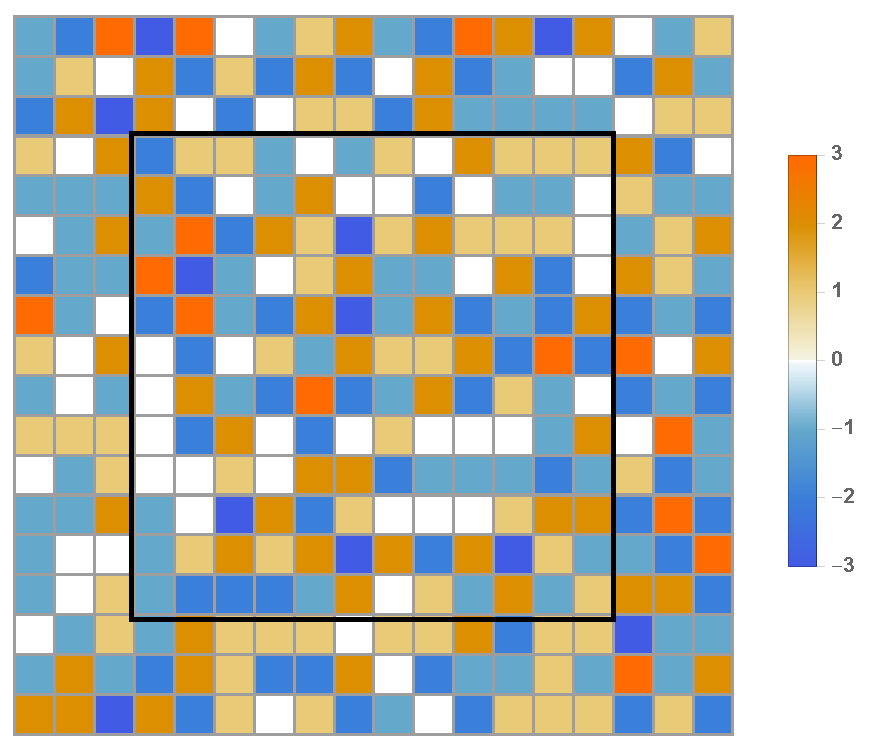
\includegraphics[width=0.40\textwidth]{HL18Shadowing12SourceA}
(b)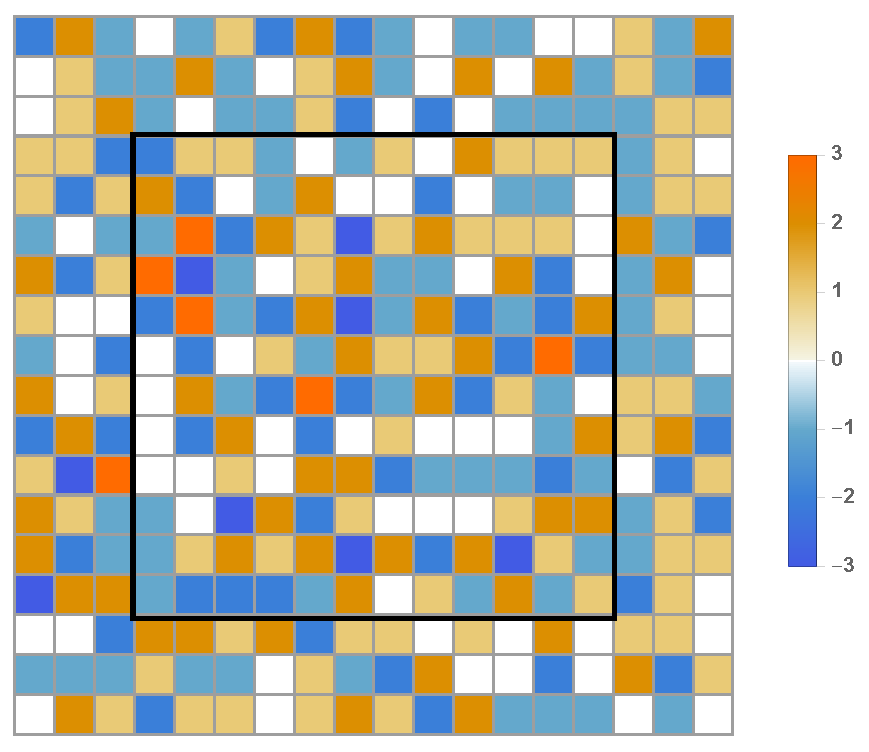
\includegraphics[width=0.40\textwidth]{HL18Shadowing12SourceB}
  \caption{\label{fig:HL18Shadowing12Source}
(a) and (b) are two {\admissible} [18$\times$18] \brick s corresponding to the two
distinct \twots\ of \reffig{fig:HL18Shadowing12Field}. They coincide within the shared
[12$\times$12] \brick\  $\Mm_\R$, region $\R$ indicated by the black border.
}
\end{figure}
%%%%%%%%%%%%%%%%%%%%%%%%%%%%%%%%%%%%%%%%%%%%%%%%%%%%%%%%%%%%%%%

%%%%%%%%%%%%%%%%%%%%%%%%%%%%%%%%%%%%%%%%%%%%%%%%%%%%%%%%%%%%%
\begin{figure}
  \centering
(a)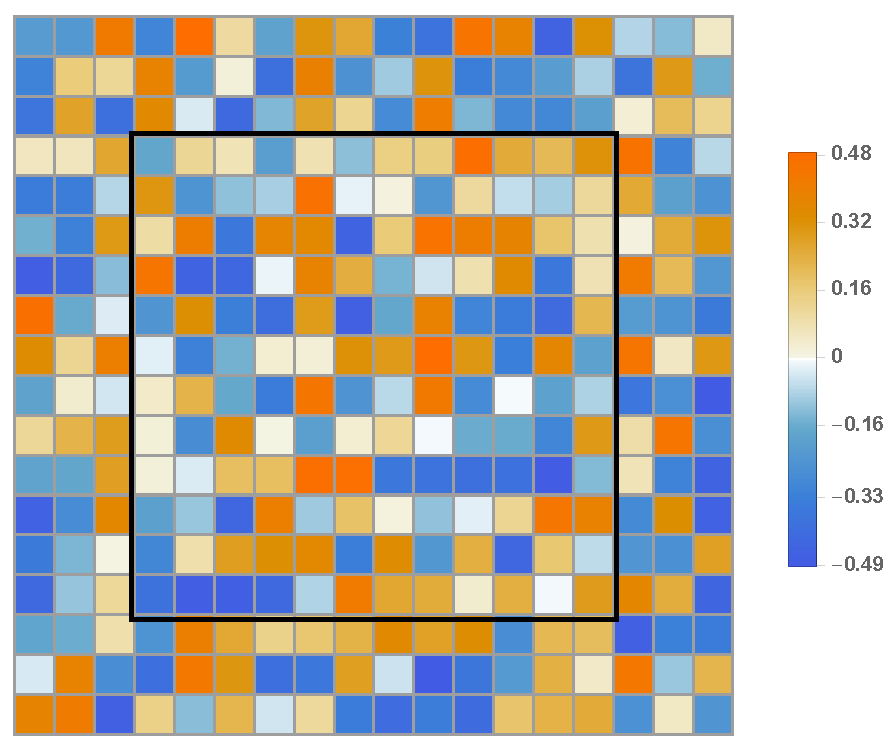
\includegraphics[width=0.40\textwidth]{HL18Shadowing12FieldA}
(b)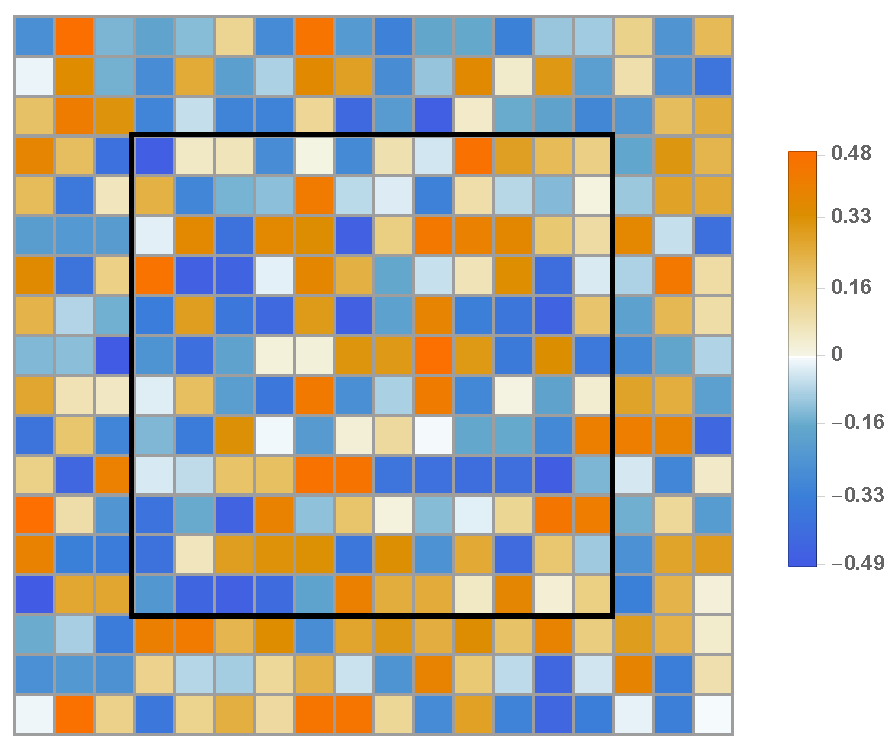
\includegraphics[width=0.40\textwidth]{HL18Shadowing12FieldB}
  \caption{\label{fig:HL18Shadowing12Field}
(a) and (b) are two \twots\ whose symbol arrays are given by the $[18\times18]$ \brick s of symbols of \reffig{fig:HL18Shadowing12Source}.
}
\end{figure}
%%%%%%%%%%%%%%%%%%%%%%%%%%%%%%%%%%%%%%%%%%%%%%%%%%%%%%%%%%%%%%%

%%%%%%%%%%%%%%%%%%%%%%%%%%%%%%%%%%%%%%%%%%%%%%%%%%%%%%%%%%%%%
\begin{figure}
  \centering
(a)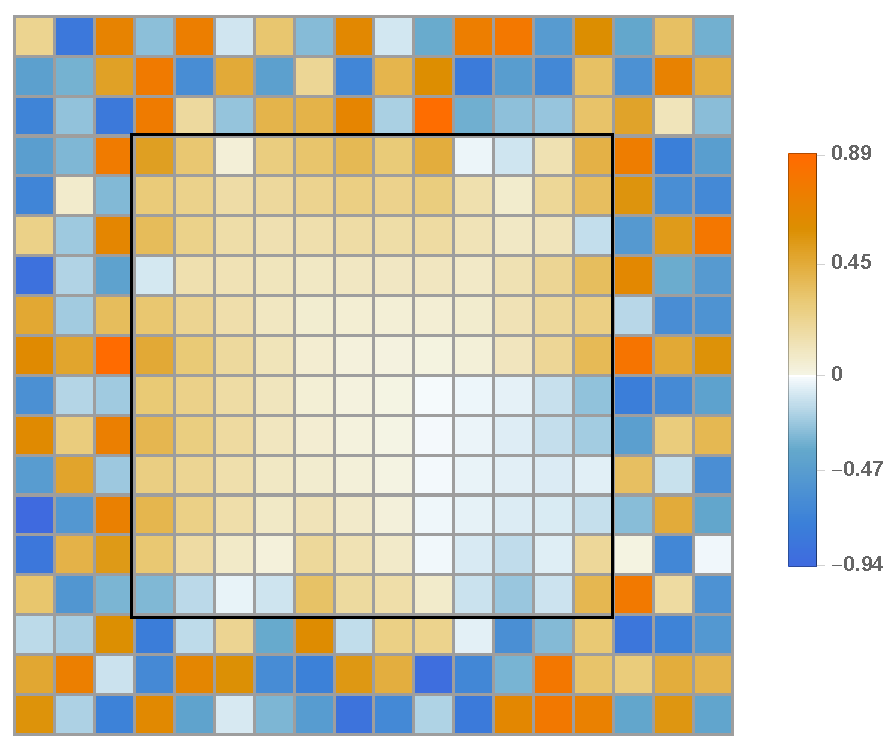
\includegraphics[width=0.40\textwidth]{HL18Shadowing12FieldDistance}
(b)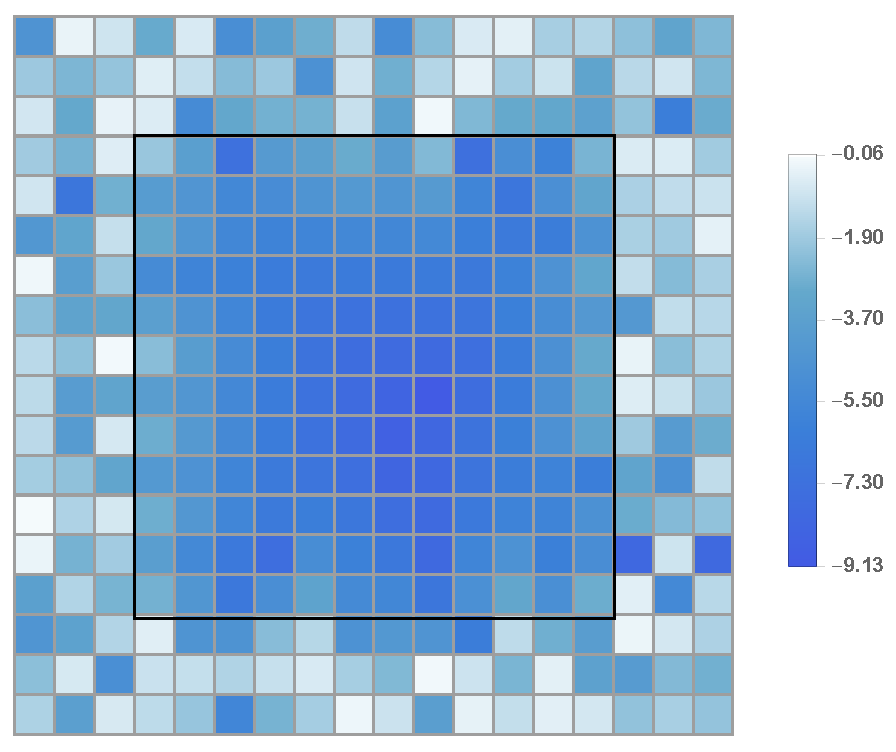
\includegraphics[width=0.40\textwidth]{HL18Shadowing12FieldDistanceLog}
  \caption{\label{fig:HL18Shadowing12Distance}
(a) The pointwise distance between the two \twots\ of \reffig{fig:HL18Shadowing12Field}.
(b) The logarithm of the absolute value of the distance between the two \twots\ indicate exponential shadowing close to the center of the shared $\Mm_\R$.
}
\end{figure}
%%%%%%%%%%%%%%%%%%%%%%%%%%%%%%%%%%%%%%%%%%%%%%%%%%%%%%%%%%%%%%%

	\HLpost{2019-08-21}{
I also did the shadowing plot of $[18\times18]$ \brick s with a smaller shared region of symbols. As shown in \reffigs{fig:HL18Shadowing8Source}{fig:HL18Shadowing8Field}, the shared region is a $[8\times8]$ \brick.

What I'm considering is: the symbols are on \twots,  so as we go further from the center of the shared region, we are getting closer to the shared region of the next tile. Using a smaller shared region we can probably reduce the effect of the next shared region. But compare \reffig{fig:HL18Shadowing12Distance} (b) and \reffig{fig:HL18Shadowing8Distance} (b), the logarithm of the distance is not too different. So I guess we don't need these figures with small shared region...

Also I think this exponential shadowing only exist in the region with shared symbols? In \reffig{fig:HL18Shadowing12Distance} (b) and \reffig{fig:HL18Shadowing8Distance} (b), the distance outside of the shared region looks random, while the distance within the shared region shrink exponentially as we go closer to the center.
	}
	
%%%%%%%%%%%%%%%%%%%%%%%%%%%%%%%%%%%%%%%%%%%%%%%%%%%%%%%%%%%%%
\begin{figure}
  \centering
(a)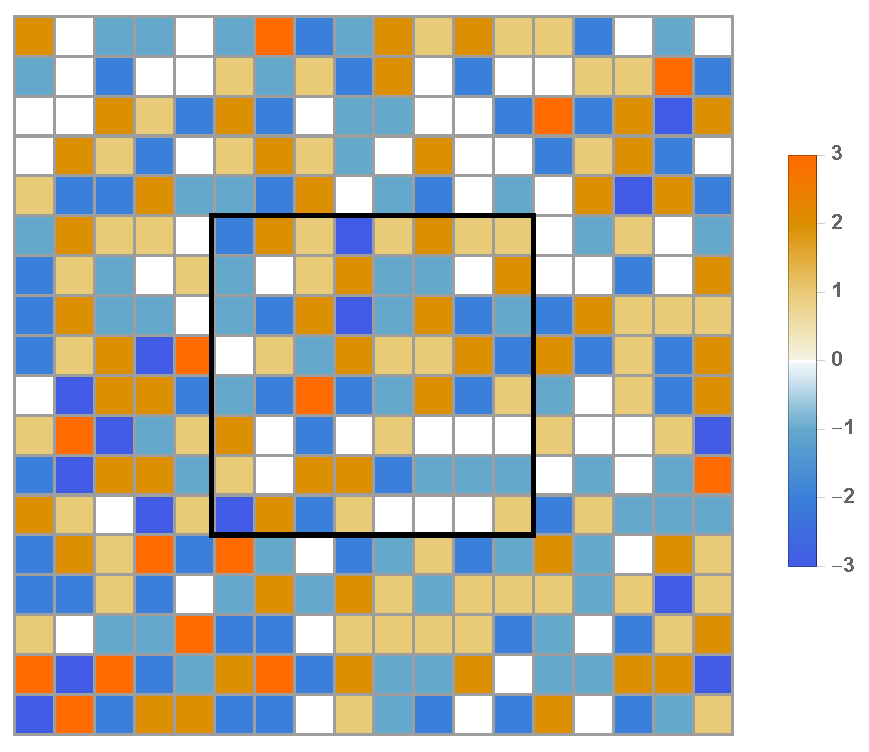
\includegraphics[width=0.40\textwidth]{HL18Shadowing8SourceA}
(b)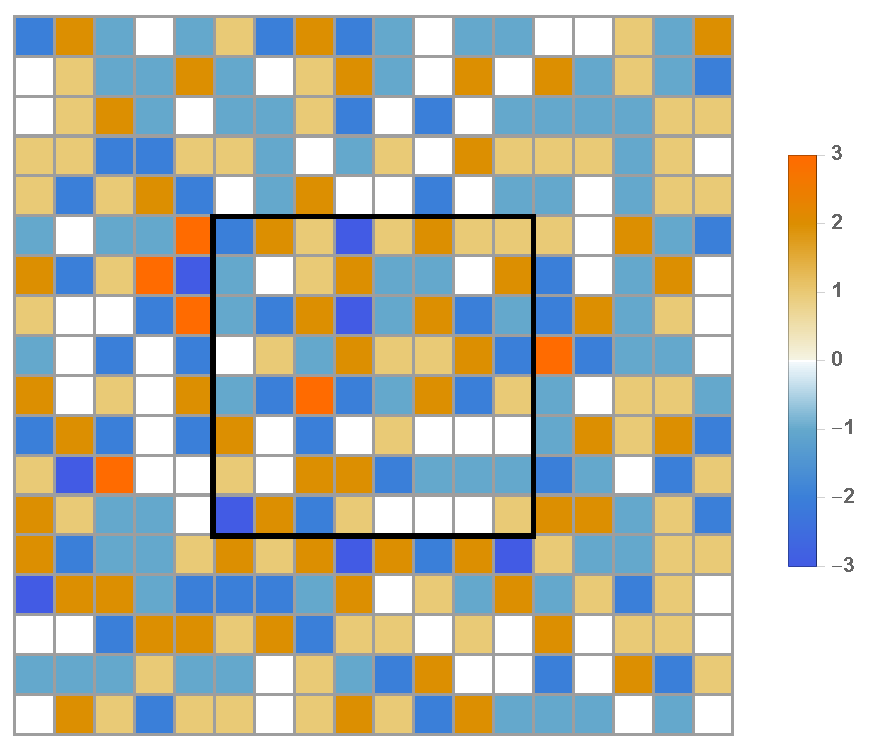
\includegraphics[width=0.40\textwidth]{HL18Shadowing8SourceB}
  \caption{\label{fig:HL18Shadowing8Source}
(a) and (b) are two {\admissible} [18$\times$18] \brick s corresponding to the two
distinct \twots\ of \reffig{fig:HL18Shadowing8Field}. They coincide within the shared
[8$\times$8] \brick\  $\Mm_\R$, region $\R$ indicated by the black border.
}
\end{figure}
%%%%%%%%%%%%%%%%%%%%%%%%%%%%%%%%%%%%%%%%%%%%%%%%%%%%%%%%%%%%%%%

%%%%%%%%%%%%%%%%%%%%%%%%%%%%%%%%%%%%%%%%%%%%%%%%%%%%%%%%%%%%%
\begin{figure}
  \centering
(a)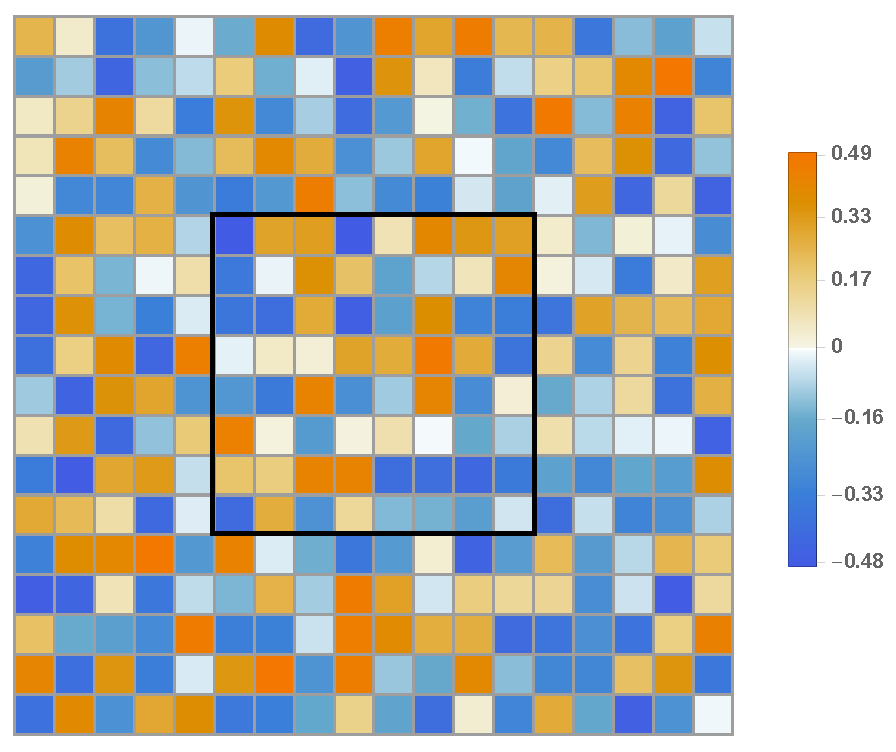
\includegraphics[width=0.40\textwidth]{HL18Shadowing8FieldA}
(b)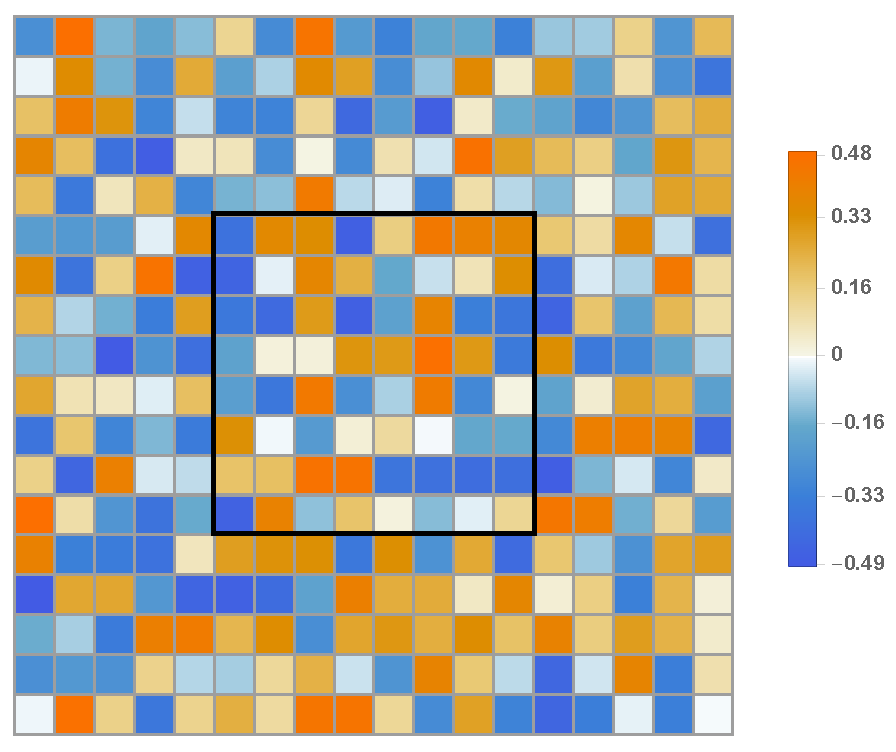
\includegraphics[width=0.40\textwidth]{HL18Shadowing8FieldB}
  \caption{\label{fig:HL18Shadowing8Field}
(a) and (b) are two \twots\ whose symbol arrays are given by the $[18\times18]$ \brick s of symbols of \reffig{fig:HL18Shadowing8Source}.
}
\end{figure}
%%%%%%%%%%%%%%%%%%%%%%%%%%%%%%%%%%%%%%%%%%%%%%%%%%%%%%%%%%%%%%%

%%%%%%%%%%%%%%%%%%%%%%%%%%%%%%%%%%%%%%%%%%%%%%%%%%%%%%%%%%%%%
\begin{figure}
  \centering
(a)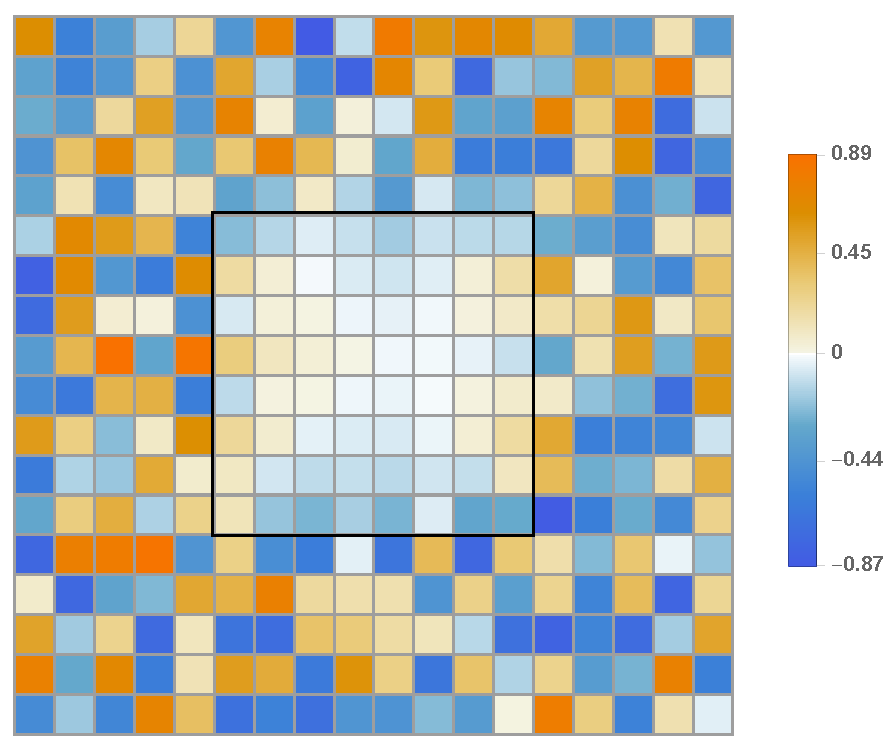
\includegraphics[width=0.40\textwidth]{HL18Shadowing8FieldDistance}
(b)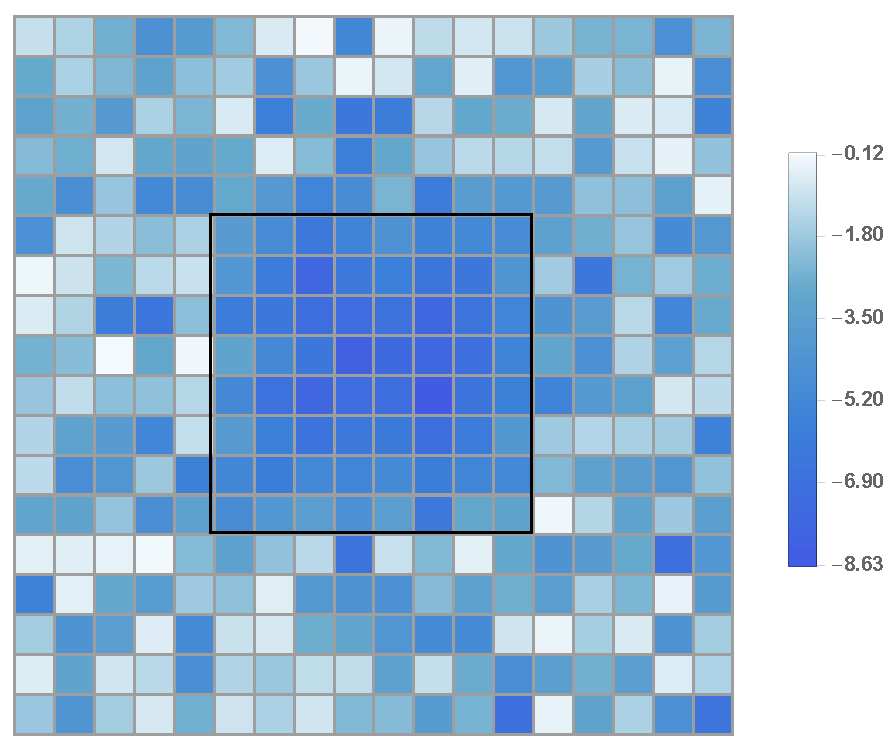
\includegraphics[width=0.40\textwidth]{HL18Shadowing8FieldDistanceLog}
  \caption{\label{fig:HL18Shadowing8Distance}
(a) The pointwise distance between the two \twots\ of \reffig{fig:HL18Shadowing8Field}.
(b) The logarithm of the absolute value of the distance between the two \twots\ indicate exponential shadowing close to the center of the shared $\Mm_\R$.
}
\end{figure}
%%%%%%%%%%%%%%%%%%%%%%%%%%%%%%%%%%%%%%%%%%%%%%%%%%%%%%%%%%%%%%%

	\HLpost{2019-08-21}{
Another thing I tried is to generate 11 different $[18\times18]$ \twots\ shared a same $[12\times12]$ \brick\ of symbols. Take one of these \twots\ and compute the distance between this \twot\ and other 10 \twots, then compute the ensemble average. The result is shown in \reffig{fig:HL18Shadowing12DistanceAverage}, which looks very similar to \reffig{fig:HL18Shadowing12Distance}. Perhaps using a larger group of ensemble we can get a better result?
	}
	
%%%%%%%%%%%%%%%%%%%%%%%%%%%%%%%%%%%%%%%%%%%%%%%%%%%%%%%%%%%%%
\begin{figure}
  \centering
(a)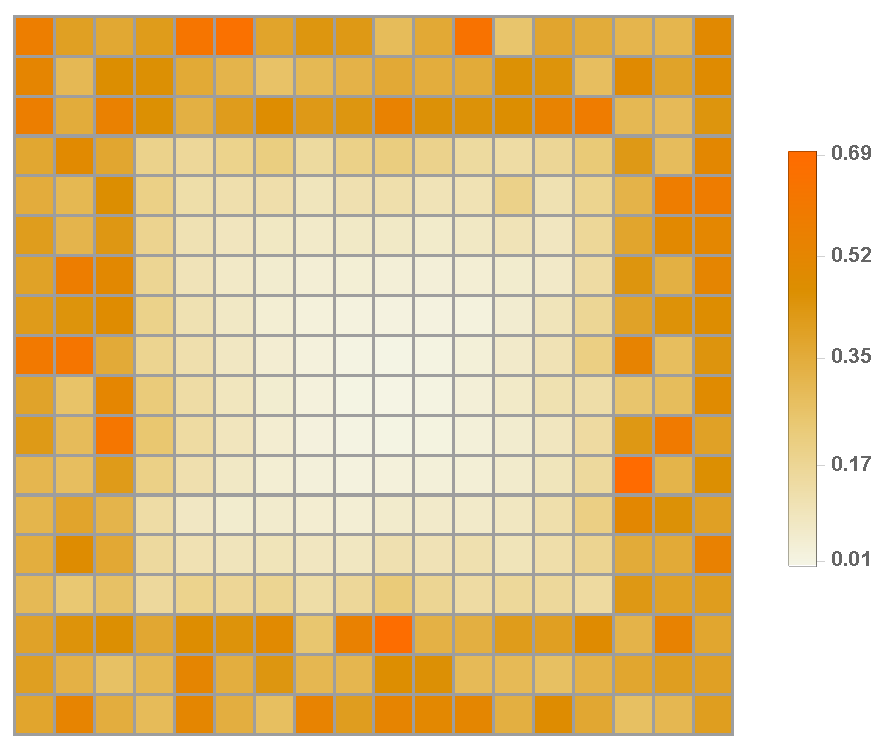
\includegraphics[width=0.40\textwidth]{HL18ShadowingDistanceAverage}
(b)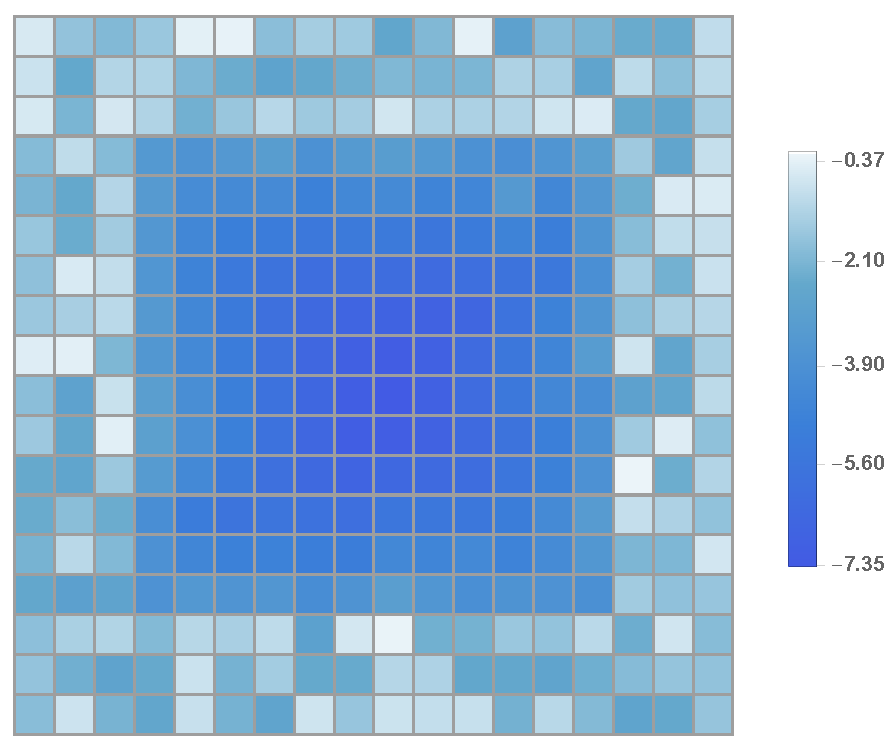
\includegraphics[width=0.40\textwidth]{HL18ShadowingDistanceAverageLog}
  \caption{\label{fig:HL18Shadowing12DistanceAverage}
(a) The average of the absolute value of the pointwise distance between the one \twot\ and other 10 different \twots\ with shared $[12\times12]$ \brick\ of symbols.
(b) The logarithm of the average of the absolute value of the distance between the \twots\ indicate exponential shadowing close to the center of the shared $\Mm_\R$.
}
\end{figure}
%%%%%%%%%%%%%%%%%%%%%%%%%%%%%%%%%%%%%%%%%%%%%%%%%%%%%%%%%%%%%%%

	\HLpost{2019-08-22}{
I generated 500 different \twots\ with a shared $[12\times12]$ \brick\ of symbols at the center, labeled as $\Xx_1, \Xx_2, \dots, \Xx_{500}$. Then I compute the distance between $\Xx_i$ and $\Xx_{i+250}$ where $i$ goes from 1 to 250, and get 250 distance field. \refFig{fig:HL18ShadowingDistanceAverage3D} is the log plot of the absolute value of the distance field. \refFig{fig:HL18ShadowingDistanceAverage3D} (a) is the logarithm of the distance between field $\Xx_1$ and $\Xx_{251}$, and (b) is the the logarithm of the average of the 250 distance field. By doing the average, the distance field becomes smooth. \refFig{fig:HL18ShadowingDistanceAverageCrossSection} is the cross section of \reffig{fig:HL18ShadowingDistanceAverage3D} through the center of the field. In \reffig{fig:HL18ShadowingDistanceAverageCrossSection} (b) the logarithm of the distance is straight line in the region with shared symbols, which shows that the distance shrink exponentially as getting closer to the center.

In \reffig{fig:HL18ShadowingDistanceAverageCrossSection} (b), the logarithm of the distance outside of the shared symbol \brick\ is approximately equal to $\ln(1/3) = -1.0986$, where $1/3$ is the average distance between two random numbers within the range $[-1/2, 1/2)$.

I still need to add axis labels to these figures... (It seems like Mathematica doesn't allow me to use LaTeX for writing the labels.)
	}

%%%%%%%%%%%%%%%%%%%%%%%%%%%%%%%%%%%%%%%%%%%%%%%%%%%%%%%%%%%%%
\begin{figure}
  \centering
(a)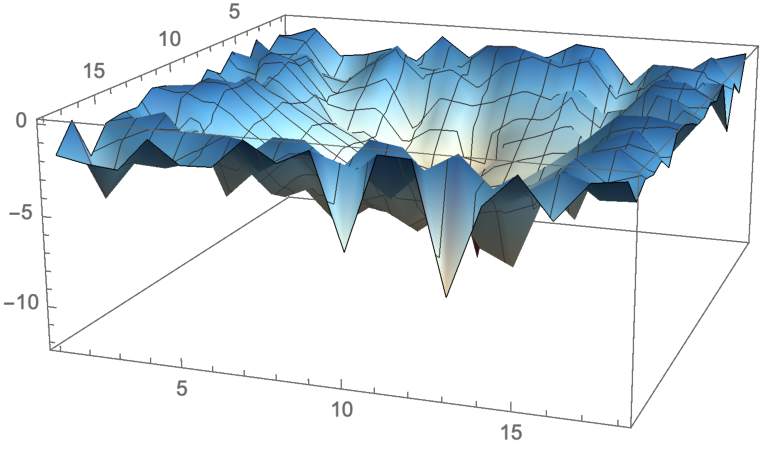
\includegraphics[width=0.40\textwidth]{HL18ShadowingDistanceLog3D}
(b)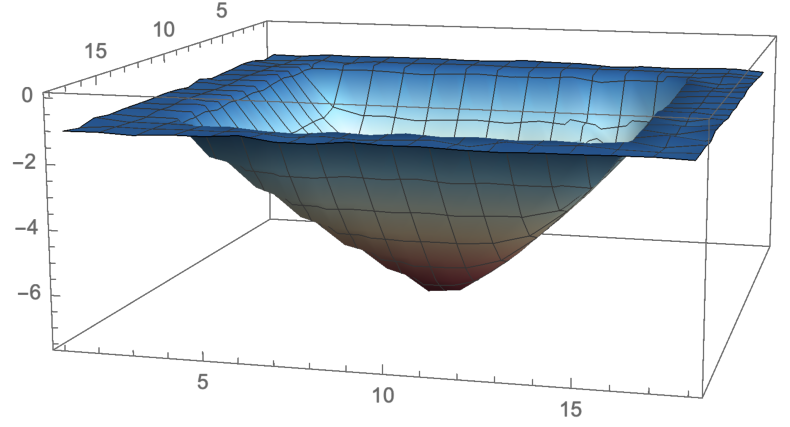
\includegraphics[width=0.40\textwidth]{HL18ShadowingDistanceAverageLog3D}
  \caption{\label{fig:HL18ShadowingDistanceAverage3D}
(a) The logarithm of the absolute value of the pointwise distance between the solutions $\Xx_1$ and $\Xx_{251}$ with shared $[12\times12]$ \brick\ of symbols at the center.
(b) The logarithm of the average of the absolute value of 250 different distance fields.
}
\end{figure}
%%%%%%%%%%%%%%%%%%%%%%%%%%%%%%%%%%%%%%%%%%%%%%%%%%%%%%%%%%%%%%%

%%%%%%%%%%%%%%%%%%%%%%%%%%%%%%%%%%%%%%%%%%%%%%%%%%%%%%%%%%%%%
\begin{figure}
  \centering
(a)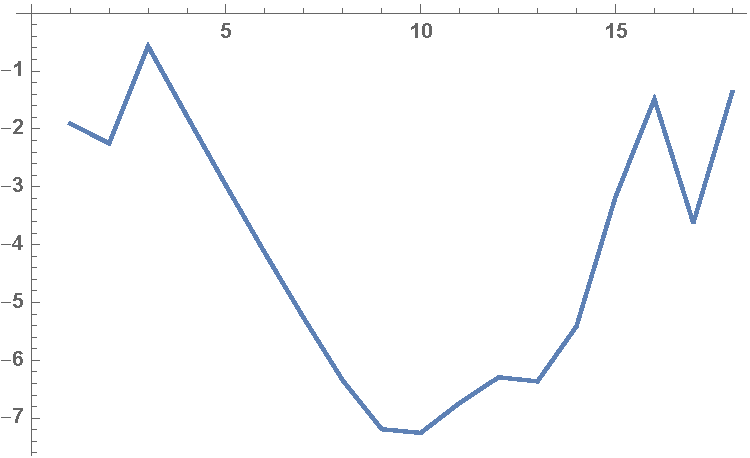
\includegraphics[width=0.40\textwidth]{HL18ShadowingDistanceLogCrossSection}
(b)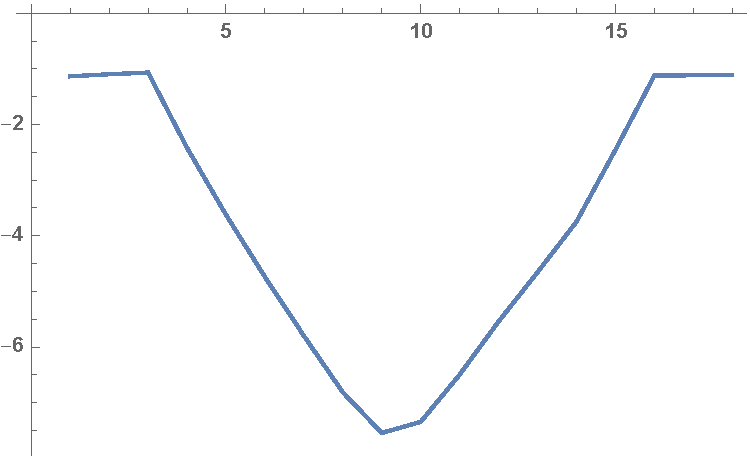
\includegraphics[width=0.40\textwidth]{HL18ShadowingDistanceAverageLogCrossSection}
  \caption{\label{fig:HL18ShadowingDistanceAverageCrossSection}
(a) The cross section through the center of the \reffig{fig:HL18ShadowingDistanceAverage3D} (a).
(b) The cross section through the center of the \reffig{fig:HL18ShadowingDistanceAverage3D} (b). The logarithm of the distance decreases linearly as the coordinate of the field approaches the center of the shared symbol \brick.
}
\end{figure}
%%%%%%%%%%%%%%%%%%%%%%%%%%%%%%%%%%%%%%%%%%%%%%%%%%%%%%%%%%%%%%%


	\PCpost{2019-09-05}{dropped this:\\
\( %\beq
(\ssp \mapsto A \ssp
    \,%\qquad
|\,
\ssp
    % = \left(\begin{array}{c} \coord\\p \end{array} \right )
  \in \mathbb{T}^2 =  \reals^2/\integers^2
    \,;\; %\qquad
A \in \SLn{2}{\integers}
)
\,,
\) %\ee{LinSympMap}

on no time-forward map,

\bigskip
In \refappe{s:GenFctn} we derive the Lagrangian formulation of cat maps.

Cat map is so simple that going from Hamiltonian to Lagrangian
formulation amounts to replacement \refeq{Ham2Lagr} of momentum
by velocity.
Still, for what follows, it might pay off to understand the general
theory of transformations from discrete Hamiltonians to discrete
Lagrangians; we review that in  refappe {s:GenFctn}.

The new results follow from our determination of \statesp\ generating partitions
generated by the iterations of the cat map, for different integer values
of the stretching parameter $s$.

, new kinds of
determinants, new relations between propagation of temporal vs. spatial
disturbances; some of these are derived in XXX eq.~{s:Green}.

the discrete
Euler–Lagrange equations \refeq{LC21eqMotion} take form of 3-term,
second-order difference equations
% \refeq{LC21:1dTempFT}
\[
- \ssp_{\zeit+1} + V'(\ssp_{\zeit}) - \ssp_{\zeit-1}
    =
\Ssym{\zeit}
\,.  %\qquad  \ssp_{\zeit} \in [0,1)
\]

Following eqs. {PerViv2.1a} and {PerViv2.1b}:
Here $2\pi \coord$ is the  angle of the rotor, $p$ is the
momentum conjugate to the angular coordinate $\coord$, the angular pulse
$P(\coord)=P(\coord+1)$ is periodic with period $1$, and the time step
has been set to $\Delta\zeit= 1$.
Eq.~\refeq{PerViv2.1b} says that in one time step $\Delta\zeit$ the
configuration trajectory starting at $\coord_{\zeit}$ reaches
$\coord_{\zeit+1} = \coord_{\zeit}+p_{\zeit+1}\Delta {\zeit}$,
and
\refeq{PerViv2.1a} says that at each kick the angular momentum
$p_{\zeit}$ is accelerated to $p_{\zeit+1}$ by the force
$P(\coord_{\zeit})\Delta\zeit$.
As the values of $\coord$ differing by integers are identified, and the
momentum $p$ is unbounded, the phase space is a cylinder. However, one
can analyze the dynamics just as well on the compactified phase space,
with the momentum wrapped around a circle, \ie, adding $\mod 1$ to
\refeq{PerViv2.1a}. Now the dynamics is a toral automorphism acting on a
$(0,1]\times(0,1]$ phase space square of unit area, with the opposite
edges identified.

We shall refer here to the least unstable of the cat maps
\refeq{catMap}, with $s=3$, as the `Arnol'd cat
map'\rf{ArnAve,deva87}, and to maps with integer $s\geq 3$ as `cat
maps'.

For {\catlatt} \refeq{CatMap2d} the field $\ssp_{n\zeit}$ takes values in
the $\speriod{}\period{}$\dmn\ unit hyper-cube
$\Xx\in[0,1)^{\speriod{}\period{}}$, where $\speriod{}$ is the `spatial',
and $\period{}$ the `temporal' lattice period.

    }

	\PCpost{2019-12-15}{move to GuBuCv17.tex:\\
Flows described by {\pdes} are in principle infinite dim\-ens\-ion\-al,
and, at first glance, turbulent dynamics that they exhibit might appear
hopelessly complex. However, what is actually observed in experiments and
simulations is that turbulence is dominated by repertoires of
identifiable recurrent vortices, rolls, streaks and the
like\rf{science04}. Dynamics on a low-dim\-ens\-ion\-al chaotic attractor
can be visualized as a succession of near visitations to exact unstable
periodic  solutions of the equations of motion, interspersed by transient
interludes\rf{DasBuch}. In the same spirit, the long-term turbulent
dynamics  of spatially   extended systems can  be thought of as a
sequence of visitations through the repertoire of {\admissible}  {\spt}
patterns, each framed by a finite {\spt}
window. The question we address here is: can states of a strongly
nonlinear field theory  be described by such repertoires of {\admissible}
patterns explored by turbulence?
And if yes, what is the likelihood to observe any such pattern?

Such  questions have been   studied  extensively for systems of  small
spatial extension, where the attractor dimension is relatively
small\rf{Christiansen97,SCD07,CviGib10,ACHKW11,KreEck12}.
However, going from  spatially small to spatially infinite systems
will require completely new tools.
For small systems the
long time dynamics can be thought of as motion of a point within an
inertial  manifold  of a moderate dimension.

    }



	\PCpost{2019-12-14}{restore this somewhere in cat map discussions:\\
The key property of hyperbolic flows is that nearby trajectories can
\emph{shadow} each other for finite times controlled by their stability
exponents. One common way to quantify `nearness' is to determine the
minimal Euclidean distance between pairs of trajectories. That kind of
distance is not invariant under symplectic transformations, and is thus
meaningless in the Hamiltonian phase space. Here the notion of action
comes to rescue:
\emph{the symplectic invariant distance between a pair of shadowing
orbits is given by the difference of their actions}\rf{LiTom17b}.
    }

    \PCpost{2019-12-20}{dropped\\
Incorporate \emph{spatiotemp/Examples/tempStab3cyc.tex},
eq.~{tempStab3cyc:inv}
    }

    \PCpost{2020-01-13}{Implemented now in the article:\\
I know LU is a method in textbooks, but in this example, cannot you use
the periodicity of $\shift$, as I do in \refsect{s:bernCount}~{\em
Counting Bernoulli \po s}, \refsect{exam:tempStab3cyc}~{\em Temporal
lattice stability of a 3-cycle}, but for $d$\dmn\ example done here?
\refeq{dDmnForwardJacobianB} is the same as \refeq{LnDet=TrLn}, but for a
$d$\dmn\ \jacobianM\ $\jMat$, rather than the $1$\dmn\ matrix ${s}$.
    }

    \PCpost{2019-08-04}{
to Han - Please make sure that all definitions and signs
agree with the discrete lattice sections of ChaosBook\rf{DasBuch}.
                    }

\HLpost{2020-01-28}{
To prove that the product of cosines gives Chebyshev polynomial, the
simplest way is to use the identity from Grashteyn and Ryzhik\rf{GraRyz}
{\em Table of Integrals, Summations and Products}
(Academic Press, New York, 1965) 1.395.2:
\beq
\cosh nx -\cos ny
  = 2^{n-1} \prod_{k=0}^{n-1} \big\{ \cosh x - \cos(y+\frac{2 k \pi}{n}) \big\}
\, .
\label{TableOfISP13952}
\eeq
Let $y=0$, $\cosh x = s/2$, and multiply both side by 2, \refeq{TableOfISP13952} becomes:
\beq
\prod_{k=0}^{n-1} \big\{ s - 2 \cos(\frac{2 k \pi}{n}) \big\}
=2 \{\cosh[n \, \mbox{arcosh}(s/2)] - 1\}
\, .
\label{TableOfISP13952-2}
\eeq
By the definition of the Chebyshev polynomials of the first kind:
\[
T_n(x) = \cosh(n \, \mbox{arcosh} \, x), \quad \mbox{if} \, x \geq 1 \, ,
\]
the right hand side of \refeq{TableOfISP13952-2} is $2\,T_{n}(s/2) -2$,
same as \refeq{POsChebyshev}.

%Using the standard theory of Toeplitz matrices (or the orthonormality of
%discrete Fourier eigenmodes, see \refappe{appe:Fourier}), one can write
%determinant \refeq{POsChebyshev} compactly as
%\beq
%N_\cl{} = \det \jMorb
% = 2\,T_{\cl{}}(s/2) -2
%% = \ExpaEig^{\cl{}} + \ExpaEig^{-\cl{}} - 2
%\,,
%\label{POsChebyshevFT}
%\eeq
%where $T_{\cl{}}(s/2)$ is the Chebyshev polynomial of the first kind.
%
%Or, without any explicit reference to Chebyshev polynomials, see
%\refeq{Isola90-13} below.
     } %\HLpost{2020-01-28}{

    \PCpost{2019-12-18}{
turn the final version into
\emph{spatiotemp/chapter/examSawtoothLin.tex} examples,
then move to ChaosBook.
    }


%    \PCpost{2019-12-24}{
%Thanks for catching my sign error.
%Is the derivation of \refeq{detBern2}
%OK now?
%    }

    \HLpost{2020-01-17}{
For
a {\lattstate} $\Xx_\Mm$ with period $\cl{}$, the \jacobianOrb\
\refeq{jacobianOrb} is a $[\cl{}d\times\cl{}d]$ block matrix
\beq
\begin{array}{cc}
 \\ \\ \jMorb & = \\ \\
\end{array}
\left(
\begin{array}{ccccc}
\id & & & & -\jMat \\
-\jMat & \id & \\
& ~~\cdots~~ & \id \\
 & & ~~\cdots~~ & \id \\
 & & &-\jMat & \id
\end{array}
\right)
= \id-\jMat \otimes \shift^{-1}
\,,
\ee{dDmnForwardJacobianB}
where $\id$ is a $d$\dmn\ identity matrix, $\jMat$ is the one time
step $[d\times d]$ \jacobianM\ \refeq{dDmn1stepJac1}, and $\shift$ is
the $[\cl{} \times \cl{}]$ {\shiftOp} matrix with period $\cl{}$.

To evaluate the determinant of the \jacobianOrb, expand $\ln \det \jMorb = \tr \ln \jMorb$:
\bea
\ln \det \jMorb
&=& \tr \ln (\id-\jMat \otimes \shift^{-1}) \continue
&=& - \sum_{k=1}^{\infty} \frac{1}{k}\tr (\jMat \otimes \shift^{-1})^k
\, .
\label{dDmnForwardJacobianLnDet}
\eea
Note that $(\jMat \otimes \shift^{-1})^k = \jMat^k \otimes \shift^{-k}$ and
$\tr (\jMat^k \otimes \shift^{-k})
= \tr (\jMat^{\cl{}r} \otimes \id_{[\cl{}\times\cl{}]}) \delta_{k,\cl{}r}
= \cl{} \tr (\jMat^{\cl{}r}) \delta_{k,\cl{}r}
$
 which is not 0 only when $k$ is a multiple of $\cl{}$.
\bea
\ln \det \jMorb
&=& - \sum_{r=1}^{\infty} \frac{\cl{} \tr (\jMat^{r\cl{}})}{r\cl{}}
 =  \tr [- \sum_{r=1}^{\infty} \frac{(\jMat^{\cl{}})^r}{r}] \continue
&=& \tr \ln (\id - \jMat^{\cl{}})
 =  \ln \det (\id - \jMat^{\cl{}})
\, .
\label{dDmnForwardJacobianLnDet2}
\eea
So the determinant of the \jacobianOrb\ is $\det \jMorb = \det (\id - \jMat^{\cl{}})$.


hence
\beq
\det \jMorb_\Mm
=
    \det(\jMat_\Mm-\id)
=
    \det(\jMat^\cl{} - \id)
\,.
\label{bernNotHill}
\eeq
}

\HLpost{2020-01-21}{
A possible problem is $\jMorb$ could be negative. And here we have the one time step
 \jacobianM\ instead of a scalar $s$ so I'm not sure if we can expand $\ln (\id-\jMat \otimes \shift^{-1})$
 as a series in $\jMat \otimes \shift^{-1}$...
}

\HLpost{2020-01-13}{
\refeq{NotHillDeterminant} is different from \refeq{bernNotHill}. I think
\refeq{NotHillDeterminant} is correct. Will check again.
}

    \PCpost{2020-01-13}{
You are right about the sign - I was hoping to avoid $N_\cl{} =
|\det \jMorb|$ in \refeq{detBern0}, but I cannot change the sign of the
matrix $\jMorb$ without making the fixed {point} condition
\refeq{tempBern} look awkward.
    }

    \PCpost{2020-01-24}{
I think (now commented out) \reffig{fig:FundPar}\,(b) was illegal - we
are not allowed to define a Bravais cell off the unit cell, on the 1/2
integer lattice. Removed, unless Han has a counterargument. It is kept
for the record in \emph{spatiotemp/chapter/catHamilton.tex}
    }

\HLpost{2020-01-21}{
A possible problem with \refeq{detDet} is that $\jMorb$ could be
negative. And here we have the one time step \jacobianM\ instead of a
scalar $s$ so I'm not sure if we can expand $\ln (\id-\jMat \otimes
\shift^{-1})$ as a series in $\jMat \otimes \shift^{-1}$...
}

    \PCpost{2020-01-27}{Dropped:
This overcounting happens if the initial unit square is on the integer
lattice. If initial states lie off the integer lattice, within the
symmetric unit square $(-1/2,1/2]\times(-1/2,1/2]$ (Wigner-Seitz cell?),
the fundamental parallelogram \reffig{fig:FundPar}\,(b) all 5 integer
points lie within the fundamental parallelogram, without any
over-counting. This is not the situation studied here, so we will not
pursue it further.

We are not aware of any useful visualizations of {\jacobianOrb}
{\fundPip} for $n > 3$ \templatt\ and 2- and $d$\dmn\
\catlatt\ of \refsect{s:catlatt}.

---------------------------------------------------------------
\[
(- \Box +s -4)_{0,0,i_2, j_2} = (\jMorb_{0,0})_{i_2, j_2} =
 \left[
 \begin{array}{ccc}
 -1 & -1 & 0 \\
 5 & -1 & -1
 \end{array}
 \right]_{i_2, j_2} \, ,
\]
\[
 (- \Box +s -4)_{0,1,i_2, j_2} = (\jMorb_{0,1})_{i_2, j_2} =
 \left[
 \begin{array}{ccc}
 5 & -1 & -1 \\
 -1 & 0 & -1
 \end{array}
 \right]_{i_2, j_2} \, ,
\]
\[
 (- \Box +s -4)_{1,0,i_2, j_2} = (\jMorb_{1,0})_{i_2, j_2} =
 \left[
 \begin{array}{ccc}
 0 & -1 & -1 \\
 -1 & 5 & -1
 \end{array}
 \right]_{i_2, j_2} \, ,
\]
\[
 (- \Box +s -4)_{1,1,i_2, j_2} = (\jMorb_{1,1})_{i_2, j_2} =
 \left[
 \begin{array}{ccc}
 -1 & 5 & -1 \\
 -1 & -1 & 0
 \end{array}
 \right]_{i_2, j_2} \, ,
\]
\[
 (- \Box +s -4)_{2,0,i_2, j_2} = (\jMorb_{2,0})_{i_2, j_2} =
 \left[
 \begin{array}{ccc}
 -1 & 0 & -1 \\
 -1 & -1 & 5
 \end{array}
 \right]_{i_2, j_2} \, ,
\]
\[
 (- \Box +s -4)_{2,1,i_2, j_2} = (\jMorb_{2,1})_{i_2, j_2} =
 \left[
 \begin{array}{ccc}
 -1 & -1 & 5 \\
 0 & -1 & -1
 \end{array}
 \right]_{i_2, j_2} \, .
\]
To diagonalize this rank-4 {\jacobianOrb} we need to use the the eigenvectors \refeq{2DEigenvector} to form a rank-4 tensor:
\[
U_{i_1,j_1,i_2,j_2}=
\exp\left(
      i\frac{2 \pi}{6}(2 i_2 i_1 - i_2 j_1 + 3 j_2 j_1)
        \right) \, .
\]
The inverse of this tensor is the conjugate transpose $U^\dagger$:
\[
(U^\dagger)_{i_1,j_1,i_2,j_2} = (U_{i_2,j_2,i_1,j_1})^* \, .
\]
The diagonalized {\jacobianOrb} is:
\[
(\jMorb_{\mathrm{diagonalized}})_{i_1,j_1,i_2,j_2}
= \sum_{i_3=0}^2 \sum_{j_3=0}^1 \sum_{i_4=0}^2 \sum_{j_4=0}^1 (U^\dagger)_{i_1,j_1,i_3,j_3} \jMorb_{i_3,j_3,i_4,j_4} U_{i_4,j_4,i_2,j_2} \, .
\]
The diagonalized {\jacobianOrb}'s element $(\jMorb_{\mathrm{diagonalized}})_{i_1,j_1,i_2,j_2}$ is not 0 only when $i_1 = i_2$ and $j_1 = j_2$. We can get the inverse of this diagonalized tensor, $\jMorb_{\mathrm{diagonalized}}^{-1}$, by changing the non-zero elements to their inverse. Then inverse of the {\jacobianOrb} is:
\[
(\jMorb^{-1})_{i_1,j_1,i_2,j_2} =
\sum_{i_3=0}^2 \sum_{j_3=0}^1 \sum_{i_4=0}^2 \sum_{j_4=0}^1 U_{i_1,j_1,i_3,j_3} (\jMorb_{\mathrm{diagonalized}}^{-1})_{i_3,j_3,i_4,j_4} (U^\dagger)_{i_4,j_4,i_2,j_2} \, .
\]
The elements of the inverse {\jacobianOrb} are:
\[
(\jMorb^{-1}_{0,0})_{i_2, j_2} = \frac{1}{35}
 \left[
 \begin{array}{ccc}
 5 & 5 & 4 \\
 11 & 5 & 5
 \end{array}
 \right]_{i_2, j_2} \, ,
\]
\[
(\jMorb^{-1}_{0,1})_{i_2, j_2} = \frac{1}{35}
 \left[
 \begin{array}{ccc}
 11 & 5 & 5 \\
 5 & 4 & 5
 \end{array}
 \right]_{i_2, j_2} \, ,
\]
\[
(\jMorb^{-1}_{1,0})_{i_2, j_2} = \frac{1}{35}
 \left[
 \begin{array}{ccc}
 4 & 5 & 5 \\
 5 & 11 & 5
 \end{array}
 \right]_{i_2, j_2} \, ,
\]
\[
(\jMorb^{-1}_{1,1})_{i_2, j_2} = \frac{1}{35}
 \left[
 \begin{array}{ccc}
 5 & 11 & 5 \\
 5 & 5 & 4
 \end{array}
 \right]_{i_2, j_2} \, ,
\]
\[
(\jMorb^{-1}_{2,0})_{i_2, j_2} = \frac{1}{35}
 \left[
 \begin{array}{ccc}
 5 & 4 & 5 \\
 5 & 5 & 11
 \end{array}
 \right]_{i_2, j_2} \, ,
\]
\[
(\jMorb^{-1}_{2,1})_{i_2, j_2} = \frac{1}{35}
 \left[
 \begin{array}{ccc}
 5 & 5 & 11 \\
 4 & 5 & 5
 \end{array}
 \right]_{i_2, j_2} \, .
\]
---------------------------------------------------------------

    }

    \PCpost{2020-01-30}{Dropped everything mentioning `Brillouin zones',
    for example   \reffig{fig:HLReciprocalLattice}\,(b);
they are OK for solid state physics, but our job is to count integer lattice
points, and Brillouin zones live off integer lattices.

Dropped: The periodicity of a periodic state  $\Xx({z})$ over a $d$\dmn\ lattice, with
the state described by repeats of a Bravais cell
spanned by basis vectors
\(({\bf a}_1,{\bf a}_2,\cdots,{\bf a}_d)\),
 \beq
\Lambda
= \left\{ \sum_{i=1}^d n_i {\bf a}_i\,\mid\,n_i \in \mathbb{Z}\right\}
\,.
\ee{dDBravaisLatt}

and combine them as columns of matrix
\beq
  \Lambda =
\left(\begin{array}{cc}
  \speriod{}&{S}\\
  0&\period{}
\end{array}\right)
\ee{Holmin12-Hermite2dOld}

\beq
\left[
\begin{array}{cc}
{\bf a}_1 & {\bf a}_2 \\
\end{array}
\right]
=
\left[
\begin{array}{cc}
 \speriod{} & {S} \\
 0 & \period{} \\
\end{array}
\right]
 \,.
\ee{2DBravaisBasis}

This is the simplest example
of a \catlatt\ tiling that is not just a 1\dmn\ {\templatt} \po\ solution
along one direction, repeated along the other.
    }


%%%%%%%%%%%%%%%%%%%%%%%%%%%%%%%%%%%%%%%%%%%%%%%%%%%%%%%%%%%%%
\begin{figure}
  \centering
% kept this(a)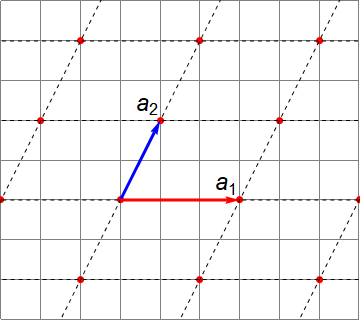
\includegraphics[width=0.40\textwidth]{HLBravaisLattice}
~~~
(b)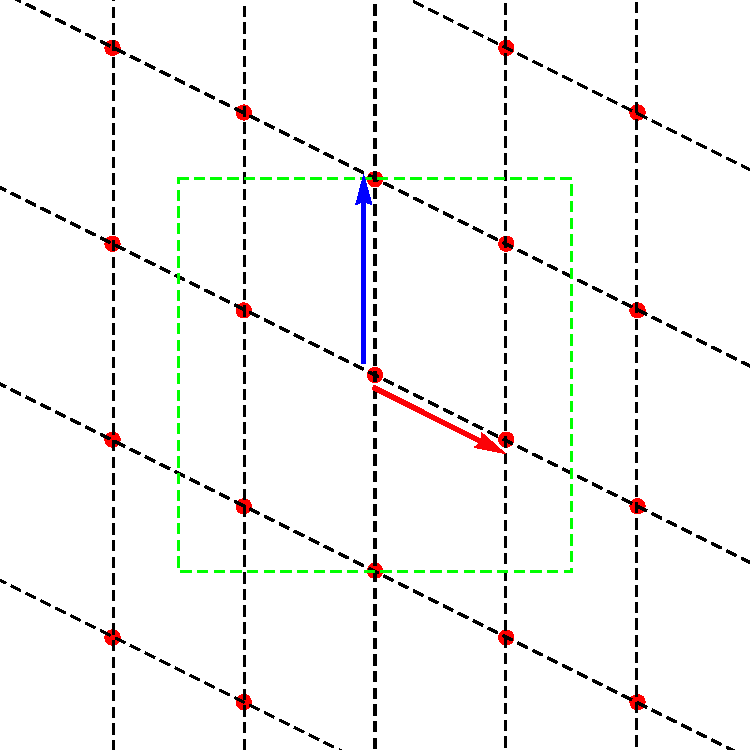
\includegraphics[width=0.40\textwidth]{HLReciprocalLattice1}
  \caption{\label{fig:HLReciprocalLattice}
%  (Color online)
(b)
    The reciprocal lattice \refeq{ReciprLattBasis}. Each reciprocal
    lattice point is a wave vector of the eigenvector of the translation
    operator with periodicity given by the Bravais lattice. The green
    dashed square encloses the first Brillouin zone of the {\em square
    lattice} (not the Bravais lattice). The wave vectors in the
    first Brillouin zone give all eigenvectors of the translation
    operator. Any wave vector outside of the first Brillouin zone is
    equivalent to a wave vector within it.
}
\end{figure}
%%%%%%%%%%%%%%%%%%%%%%%%%%%%%%%%%%%%%%%%%%%%%%%%%%%%%%%%%%%%%%%

    \PCpost {2019-09-11}{
Perhaps - if that helps:
copy to here the nomenclature used in \emph{PHYS-7143-19 week8}.
    }

    \PCpost{2019-11-24}{
    Do you have a closed form formula for counting these?
    We will need to include it in the paper. My
    $[2\!\times\!2]$ count
\(36 =
9+8+7+\cdots+1
\)
    was wrong.}

    \PCpost{2018-12-01}{ % 2020-01-11}{
Keep it as elementary as possible. Look at the beginning of the
\HREF{https://en.wikipedia.org/wiki/Chebyshev_polynomials} {wiki} - you can
already see our zeta function there. We need none of these funky trigonometric functions,
we only need the recurrence relations - they either already in this wiki, or in blogCats.tex,
or referred to in blogCats.tex.
    }

%\HLpost{2018-12-06}{
%I have a different way to prove \refeq{TableOfISP13952-2}. By the definition of the Chebyshev polynomials of the first kind:
%$\cos(n \theta) = T_n(\cos \theta)$, we can see that:
%\[
%T_\period{}\left[\cos\left(\frac{2 \pi j}{\period{}}\right)\right] = \cos(2\pi j) = 1 \, .
%\]
%So $\cos(2 \pi j /\period{})$, $j=0,1,...,\period{}-1$ are the roots of equation:
%\[
%T_n(x)-1=0 \, .
%\]
%So we have the identity:
%\beq
%T_n(x)-1 = 2^{\period{}-1} \prod_{j=0}^{\period{}-1} \left[x - \cos\left(\frac{2 \pi j }{\period{}}\right) \right]
%\, .
%\label{ProductToChebyshev}
%\eeq
%There is a coefficient $2^{\period{}-1}$ because the leading term in $T_n(x)$ is $2^{\period{}-1} x^\period{}$. Let $x=s/2$, and multiply both sides by 2, \refeq{ProductToChebyshev} becomes:
%\beq
%2T_n(s/2) - 2 = \prod_{j=0}^{\period{}-1} \left[s - 2\cos\left(\frac{2 \pi j }{\period{}}\right) \right]
%\, .
%\label{ProductToChebyshev-2}
%\eeq
%}

%%%%%%%%%%%%%%%%%%%%%%%%%%%%%%%%%%%%%%%%%%%%%%%%%%%%%%%%%%%%%
\begin{figure}
  \centering
(a)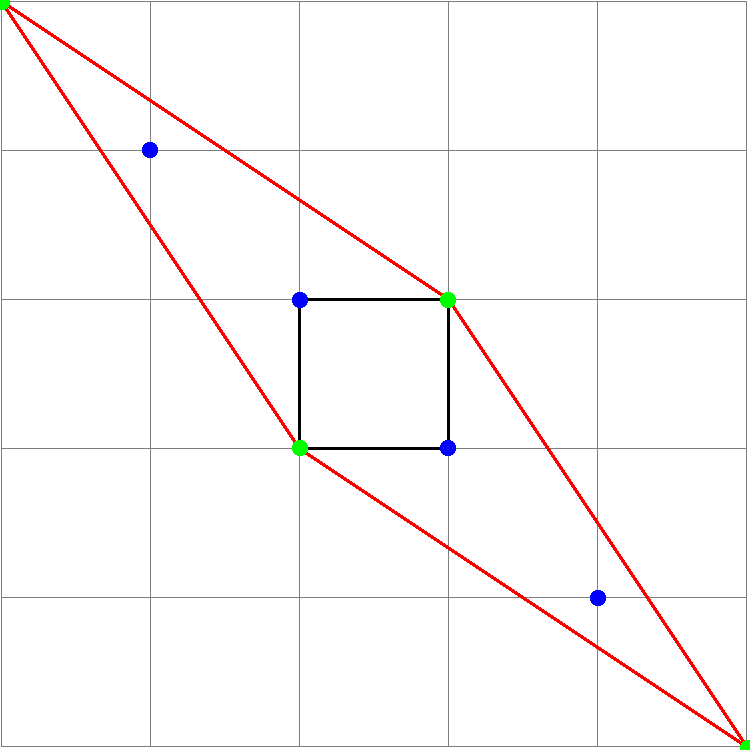
\includegraphics[width=0.45\textwidth]{HLLength2Counting}
(b)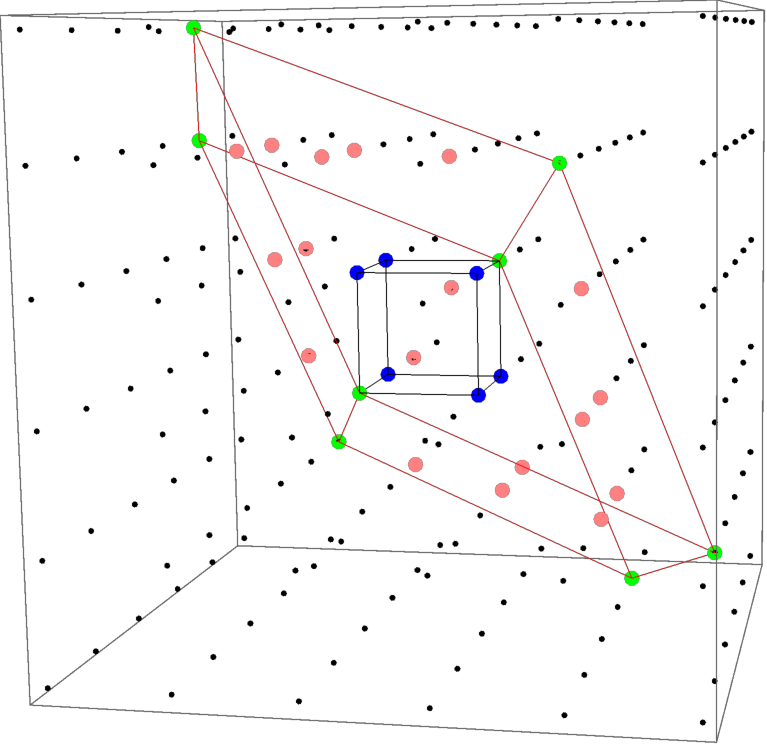
\includegraphics[width=0.45\textwidth]{HLLength3Counting-7210}
  \caption{\label{fig:HLCountingFigures}
(a) A 2-dimensional torus (with black border) stretched by $\jMorb$.
    The {\color{blue} blue} dots are internal integer points in the
    {\fundPip} (with red border). The {\color{green} green}
    dots are on the vertices of the {\fundPip}.
(b) A 3-dimensional torus (with black border) stretched by $\jMorb$.
    The {\color{blue} blue} dots are internal integer points in the
    stretched {\fundPip} (with red border). The {\color{green} green}
    dots are on the vertices of the {\fundPip}. The {
    pink} dots are on the surface of the {\fundPip}.
}
\end{figure}
%%%%%%%%%%%%%%%%%%%%%%%%%%%%%%%%%%%%%%%%%%%%%%%%%%%%%%%%%%%%%%%

%%%%%%%%%%%%%%%%%%%%%%%%%%%%%%%%%%%%%%%%%%%%%%%%%%%%%%%%%%%%%
% Predrag 2020-02-08 replaced Han's uneditable
% {HLLength2Counting}.pdf by catCyc2Jacob.svg
\begin{figure}
  \centering
(a)~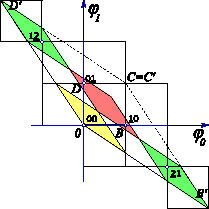
\includegraphics[width=0.35\textwidth]{catCyc2Jacob}
~~~
(b)~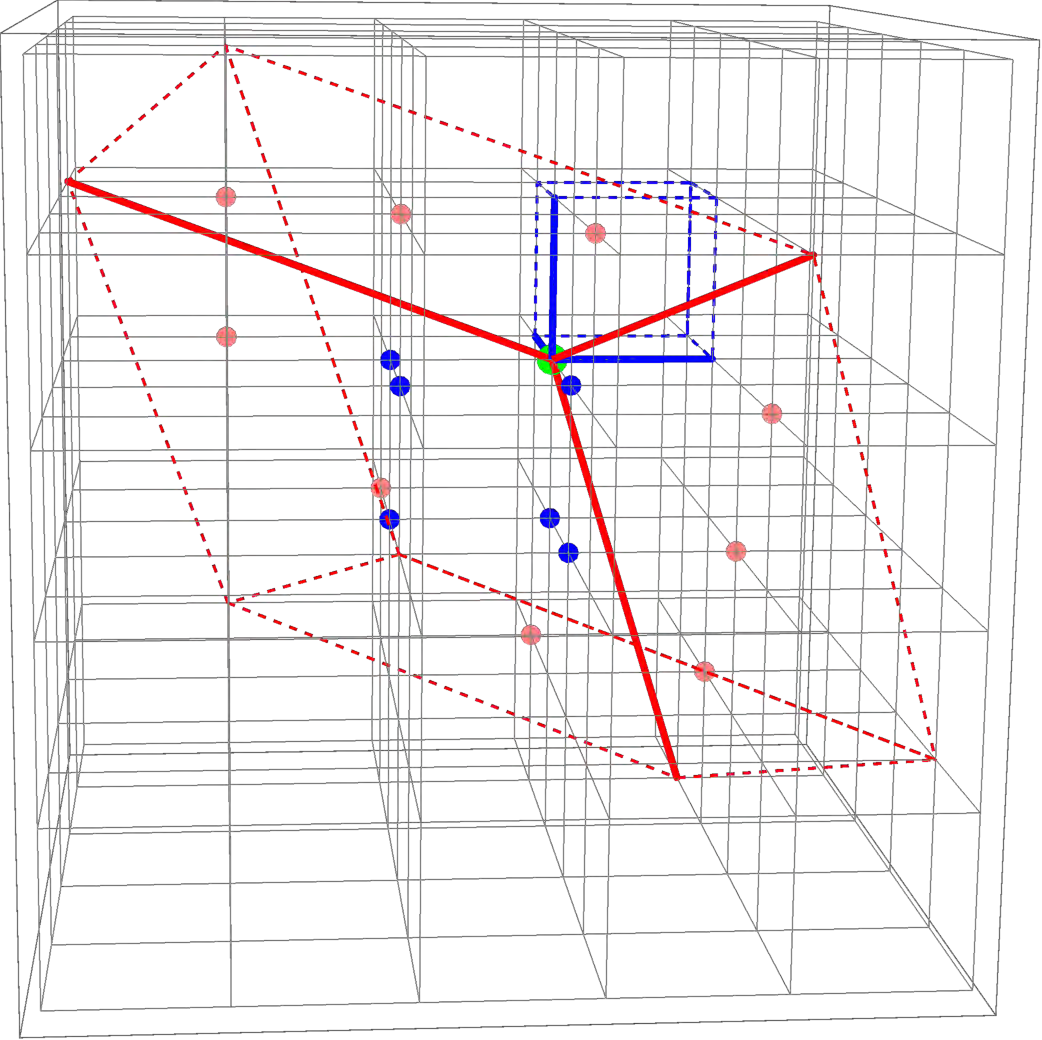
\includegraphics[width=0.40\textwidth]{HLLength3Counting}
  \caption{\label{fig:catCycJacobOld}
Was \reffig{fig:catCycJacob}, now superannuated:
(a)
    $[2\!\times\!2]$ {\jacobianOrb} $\jMorb$ \refeq{catFundPar2}
    had a wrong sign, meaningless partition into 9 rectangles.
(b) Han 2020-02-11: Intermediate attempt to draw \reffig{fig:catCycJacob}.
$[3\!\times\!3]$ {\jacobianOrb} $\jMorb$  had tons of irrelevant points plotted,
    is unintelligible.
}
\end{figure}
%%%%%%%%%%%%%%%%%%%%%%%%%%%%%%%%%%%%%%%%%%%%%%%%%%%%%%%%%%%%%%%

    \PCpost{2020-0131}{
Maybe if you plot only the points within (inside, and on the 3 faces
connected to the origin) the {\fundPip} of
\reffig{fig:catCycJacob}, no other integer points, it might be easier
to understand. Also, if you trace out the cubic lattice in light gray, it
will be clear the periodic points are on the integer lattice, in the
spirit of \reffig{fig:BernCyc2Jacob}\,(b).
    }

    \PCpost{2020-02-08}{
To Han: not writing up what you are working on in the blog is
self-defeating, as I cannot help you as long as I am not aware of you
doing anything. However, not saving figure-generating code in
\emph{siminos/mathematica} is also inefficient, as you are making me
regenerate all figures from scratch.
    }

    \PCpost{2018-06-21}{
Your difficulty is that you keep on thinking in Hamiltonian way, where
one steps in time, using the Hamilton's equations for $(q_t,p_t)$, where
we had replaced the momentum $p_t$ (at spatial position $\ell$) by
velocity $p_t=(\ssp_{\ell t}-\ssp_{\ell,t-1})/\Delta t$, and thus
initializing the Hamiltonian, a second-order difference equation for
\emph{evolution in time} by two horizontal rows $(\ssp_{\ell
t},\ssp_{\ell,t-1})\,,\;\ell\in\integers$ in the spacetime plane.

You have to think in the spacetime, Lagrangian way instead. On each
lattice site $z=(\ell,t)$ there is a scalar field $\ssp_{\ell t}$, not a
two-torus. The field $\ssp_{\ell,t-1}$ belongs to a neighboring site
$z=(\ell,t-1)$. The two fields do not form a dynamical system on a
two-torus, as the dynamics is also influenced by spatial neighbors
$\ssp_{\ell\pm1, t}$.
    }

\PCpost{2017-09-16}{
%%%%%%%%%%%%%%%%%%%%%%%%%%%%%%%%%%%%%%%%%%%%%%%%%%%%%%%%%%%%%%%%%%%%%%%%
Methods described above make it an easy task to obtain a
particular class of \twots\ for  the {\catlatt}.

\twoT's
coordinate representation $\Gamma=\{\ssp_z, z\in \ZLT\}$, is obtained by
taking inverse of \refeq{2dCoupledCats}:
  \begin{equation}
   \ssp_z=\sum_{z'\in \ZLT} \gp_{zz'} \Ssym{z'}, \qquad    \Ssym{z'}\in \Ai,
  \end{equation}
where $\gp_{zz'}$ is the corresponding Green's function with periodic
{\bcs}.
%%%%%%%%%%%%%%%%%%%%%%%%%%%%%%%%%%%%%%%%%%%%%%%%%%%%%%%%%%%%%%%%%%%%%%%%
    } %end \PCpost

    \PCpost{2018-12-01}{
Include here the song and dance from the remark.
    \\
    What Hill's formula? Is it
    \refeq{MacMei83(17)}? Not any longer sure that
     \rf{MacMei83} contains the Hill's formula...


discrete Hill's formula\rf{BolTre10}:
\beq
\det(\jMat_\Mm - \id) = \frac{(-1)^n \det \jMorb_\Mm}{\prod_{i=1}^n \det B_i}
\,,
\ee{BolTre10(2.8)a}
where for the one dimensional cat map the $B$ here is an $\BravCell{1}{1}{0}$ matrix:
\beq
B = - \frac{\delta^2 \genF[\ssp_{n+1},\ssp_{n}]}{\delta \ssp_{n+1} \delta \ssp_{n}} = 1
\,,
\ee{BolTre10(2.2)a}
    }


    \PCpost{2020-02-02}{
It is hard to find \refeq{LinearCatLatt} in {\GO}\rf{GutOsi15}. The paper
is mostly about the Hamiltonian formulation. Their (3.4) is the equation,
once on sets $c=d$ space-time isotropy, and drops their potential $V$.
Their perturbed equation (7.1) comes close to it. Their action (3.9) is a
bit mysterious as well.

Gutkin and Osipov\rf{GutOsi15}
refer to an \sPe\ \twot\ solution $p$ as a `many-particle periodic orbit', with
$\ssp_{n\zeit}$ `doubly-periodic', or `closed,'
\[
\ssp_{n\zeit} = \ssp_{n+\speriod{p},\zeit+\period{p}}
    \,,\quad
n = 0,1,2,\cdots, \speriod{p}-1
    \,;\quad
\zeit = 0,1,2,\cdots, \period{p}-1
    \,.
\]
    }

    \PCpost{2020-02-02}{
Note that in \refeq{catLatt} and throughout I have redefined the
stretching parameter ${s}$ to be stretching per dimension, \ie, ${s}$ in
\refeq{CatMap2d} is replaced by $d{s}$. This is consistent with
how one defines a diffusion constant on an isotropic $d$\dmn\ hypercubic
lattice.
    }

	\PCpost{2019-08-06}{% Is the lattice cell called the primitive cell?
    I do not think ``lattice cell'' is the standard terminology, and as
    you have chosen not to quotient the point group, what you have is not
    `primitive' - that would be 1/8th triangle that tiles the first
    Brillouin zone, I think. Please strictly follow the nomenclature of a
    single reference -presumably Dresselhaus \etal\rf{Dresselhaus07}, or
    Barvinok\rf{Barvinok08} or whatever  - and state so clearly in your
    text. Whenever you use a reference, ethics of the profession requires
    that you clearly cite it.
       }

    \HLpost{2020-02-20}{
\refFig{fig:HLfundPip2by1_1} is the \fundPip\ of a $[2\!\times\!1]_1$
\twot. The pattern of this periodic state is shown in \reffig{fig:2x1rpo}
(a). The \jacobianOrb\ of this \twot\ can be written as a
$[2\!\times\!2]$ matrix:
\[
    \jMorb
    =
     \left(\begin{array}{cc}
 -2s &  4 \\
  4 & -2s
 \end{array} \right) \, .
    \]
The shape of the \fundPip\ is very similar to \reffig{fig:catCycJacob} (a).
    }
%%%%%%%%%%%%%%%%%%%%%%%%%%%%%%%%%%%%%%%%%%%%%%%%%%%%%%%%%%%%%%%%%%
%\FIG{
\begin{figure}
  \centering
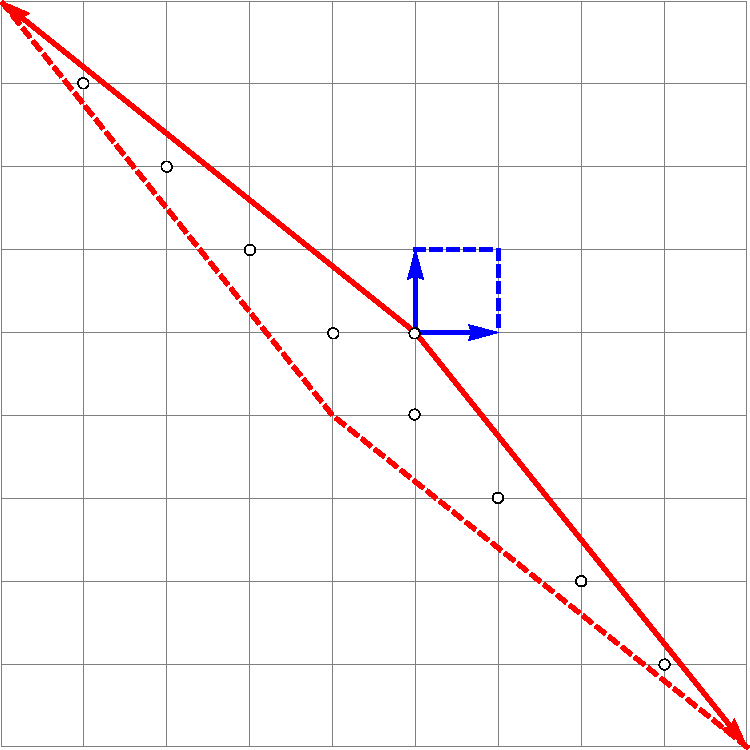
\includegraphics[width=0.40\textwidth]{HLfundPip2by1_1}
  \caption{\label{fig:HLfundPip2by1_1}
The \fundPip\ of a $[2\!\times\!1]_1$ \twot\ with $s=5/2$. Admissible field values lie within the unit square with blue boundaries. This unit square is stretched by the \jacobianOrb\ $\jMorb$ into the \fundPip\ with red boundaries. Integer points in the \fundPip\ are marked by the circles. There are 9 integer points in the \fundPip, in agreement with the counting formula.
            }
\end{figure}
%%%%%%%%%%%%%%%%%%%%%%%%%%%%%%%%%%%%%%%%%%%%%%%%%%%%%%%%%%%%%%%%%%

    \PCpost{2018-12-13}{
Must rethink the DIMENSION of $F[\Xx]$ and $\jMorb$. $F[\Xx]_i$
is a $\cl{}$\dmn\ vector function - is it dimensionally the same as
$\ssp_j$? Otherwise \jacobianOrb\ is not dimensionless, and cannot be
referred to as a `Jacobian'. Relation \refeq{detDet} only makes sense for
the dimensionless case. I think we are OK, but we have to be sure.
    }



    \PCpost{2019-08-11}{
to Han: this is wrong alphabet, for the
symmetric unit interval $\ssp\in[-1/2,1/2)$.
For all our examples we pick
the `least stretching' \catlatt\ with $s=5/2$,
with 9-letter alphabet
\beq
\A=\{\underline{4},\underline{3},\underline{2},\underline{1},
     0,1,2,3,4\}
\,.
\ee{catLattAlphabet}
    }

    \PCpost{2020-02-17}{
Now in \reftab{tab:LxTs}:
\bea
N_{\BravCell{1}{1}{0}}({s}) = 2({s}-2)
    \continue
N_{[2\!\times\!1]}({s}) = 4({s}-2)s
    \continue
N_{[2\!\times\!1]_1}({s}) = 4({s}-2)({s}+2)
    \continue
N_{[2\!\times\!2]}({s}) = 16({s}-2)s^2({s}+2)
    \continue
N_{\BravCell{3}{2}{0}}({s}) = 4({s}-2)s(2{s}-1)^2 (2{s}+3)^2
    \continue
N_{\BravCell{3}{2}{1}}({s}) = 64({s}-2){s}^3 ({s}+1)^2
    \continue
N_{\BravCell{3}{2}{2}}({s}) = 64({s}-2){s}^3 ({s}+1)^2
    \continue
N_{[3\!\times\!3]}({s}) = -32({s}-2)({s}+1)^4(2{s}-1)^4
\,.
\label{PC[LxT]volume}
\eea
    }

    \PCpost{2019-11-23}{Dropped:
For all our examples we pick
the `least stretching' hyperbolic \catlatt\ with $s=5$,
and restrict the
admissible field values $\ssp_{z}$ at lattice site $z=(n_1,n_2)$ to the
symmetric unit interval $\ssp\in[-1/2,1/2)$, with 9-letter alphabet
\refeq{catLattAlphabet}

the code depends on the choice of the unit interval:
the alphabet \A\ for $\ssp_{\zeit} \in [-1/2,1/2)$
differs from the alphabet for  $\ssp_{\zeit} \in [0,1)$.

Here $s=5/2$ and $\ssp_z\in[-1/2,1/2)$, so the
interior alphabet is one letter alphabet $\Ai=\{0\}$...

    }

%    \PCpost{2020-02-24}{
%Thanks for fixing \reftab{tab:LxTs=5/2} and \reftab{tab:LxTs}. Apparently
%I am not evaluating \emph{Tensors.nb} correctly - you'll show me how.
%    }


    \PCpost{2020-02-08}{
I think the $N_\cl{}=({s}-2)\cdots$ factorization is true for all $\cl{}$
in \refeq{1stChebGenF} and \reftab{tab:LxTs}. Do you understand it? Does
in the \templatt\ $s=2$ case, the Laplacian has a zero mode? A constant
$\ssp_i$ eigenvector? If so, why doesn't the \catlatt\ have
$N=({s}-2)^2\cdots$, one for each direction? Instead, one gets only a factor 2,
$N=2({s}-2)\cdots$.
    }

%    \PCpost{2020-02-24}{
%I had naively thought that $N_{\BravCell{\speriod{}}{1}{0}}$ families were
%the same as the 1\dmn\ \templatt\ \refeq{1stChebGenF}. Apparently not. Do
%you see something like a Chebyshev series here, or generating function
%similar to \refeq{Isola90-13}? If we cannot figure the bivariate zeta
%function, at least this family should work out?
%    }

    \PCpost{2020-02-24}{
Not urgent, but can you complete the primitive counts
$M_{[\speriod{}\!\times\!\period{}]_S}$ and decompositions of
$N_{[\speriod{}\!\times\!\period{}]_S}$ into primitive \twots\ in
\reftab{tab:LxTs=5/2} and perhaps also in \reftab{tab:LxTs}?
    }


    \PCpost{2020-03-05}{\tempLatt\ counting (all messed up,
    fix using \\ \emph{CatMaptopZeta.nb} output):
\bea
\sum_{{n}=0}^\infty N_{n} z^{n}
    & = & \frac{2-{s}z}{1 - s z + z^2}-\frac{2}{1 - z}
    \continue
\{N_{n}\} & = & s-2,s^2-4,
       s^3-3s-2,
        s^4-4s^2,
    \ceq
        2 \left(s^5-4 s^3+3 s\right)-s \left(s^4-3 s^2+1\right)-2,
    \ceq
        -2 \left(s^3-2s\right)-s\left(s^4-3 s^2+1\right)
    \ceq
-2 - s (-1 + 6 s^2 - 5 s^4 + s^6) + 2 (-4 s + 10 s^3 - 6 s^5 + s^7),
    \ceq
        -2s \left(s^5-4 s^3+3 s\right)-2 \left(s^4-3s^2+1\right)-2,
    \ceq
        -2 \left(s^5-4 s^3+3 s\right)
        +s \left(s^6-5 s^4+6s^2-1\right)-2,
        %s \left(s^7-6 s^5+10 s^3-4 s\right)-2 \left(s^6-5 s^4+6
%s^2-1\right)-2,-2 \left(s^7-6 s^5+10 s^3-4 s\right)+s \left(s^8-7 s^6+15
%s^4-10 s^2+1\right)-2,s \left(s^9-8 s^7+21 s^5-20 s^3+5 s\right)-2
%\left(s^8-7 s^6+15 s^4-10 s^2+1\right)-2,-2 \left(s^9-8 s^7+21 s^5-20
%s^3+5 s\right)+s \left(s^{10}-9 s^8+28 s^6-35 s^4+15 s^2-1\right)-2,s
%\left(s^{11}-10 s^9+36 s^7-56 s^5+35 s^3-6 s\right)-2 \left(s^{10}-9
%s^8+28 s^6-35 s^4+15 s^2-1\right)-2
\,,
\label{1stChebGenFdrop}
\eea
    }

     \PCpost{2020-03-23} {
Lot's of headless \KSe\ floundering in preparing \emph{BlogCats.tex}
\refsect{sect:KSe} saved below. Hopefully the resulting discretized \KSe\
\refeq{KSdiscr5} is correct...

\medskip

The discretized \KSe\ is of the form
\beq
\pde_\zeit \mathsf{U} + \frac{\alpha}{2}\pde_x\mathsf{U}^2
  - \beta\,\Laplacian_x \mathsf{U} + \gamma\,\Laplacian_x^2 \mathsf{U}
= 0
\,.
\ee{KSdiscr1}
Rescale $\mathsf{U}\to\mathsf{U}/\Delta\zeit$
%, divide by $\Delta x$:
\beq
\frac{\pde_\zeit}{\Delta\zeit}\mathsf{U}
+ \frac{(\Delta x)^2}{\Delta\zeit}\frac{\alpha}{2}\frac{\pde_x}{\Delta x}\mathsf{U}^2
  - \frac{(\Delta x)^2}{\Delta\zeit}\beta\,\frac{\Laplacian_x}{(\Delta x)^2} \mathsf{U}
  + \frac{(\Delta x)^4}{\Delta\zeit}\gamma\,\frac{\Laplacian_x^2}{(\Delta x)^4}\mathsf{U}
= 0
\,.
\ee{KSdiscr2}
Our canonical choice is setting these
\beq
\alpha=\frac{\Delta\zeit}{(\Delta x)^2}
    \,,\quad
\beta=-\frac{\Delta\zeit}{(\Delta x)^2}
    \,,\quad
\gamma=\frac{\Delta\zeit}{(\Delta x)^4}
\,,
\ee{KSscales}
equal to 1, parametrazing the problem with
$\speriod{}=1/\Delta x$, $\period{}=1/\Delta\zeit$,
\beq
\frac{1}{\period{}}\frac{\pde_\zeit}{\Delta\zeit} \mathsf{U}
  + \frac{1}{\speriod{}}\frac{\alpha}{2}\frac{\pde_x}{\Delta x}\mathsf{U}^2
  - \frac{1}{\speriod{}^2}\beta\,\frac{\Laplacian_x}{(\Delta x)^2} \mathsf{U}
  + \frac{1}{\speriod{}^4}\gamma\,\frac{\Laplacian_x^2}{(\Delta x)^4}\mathsf{U}
= 0
\,.
\ee{KSdiscr3}
Rescale $\mathsf{U}\to\mathsf{U}\,\period{}$
\beq
\frac{\pde_\zeit}{\Delta\zeit} \mathsf{U}
  + \frac{\period{}^2}{\speriod{}}\frac{\alpha}{2}\frac{\pde_x}{\Delta x}\mathsf{U}^2
  - \frac{\period{}}{\speriod{}^2}\beta\,\frac{\Laplacian_x}{(\Delta x)^2} \mathsf{U}
  + \frac{\period{}}{\speriod{}^4}\gamma\,\frac{\Laplacian_x^2}{(\Delta x)^4}\mathsf{U}
= 0
\,.
\ee{KSdiscr4}
Our canonical choice is setting these
\beq
\alpha=\speriod{}/\period{}^2
    \,,\quad
\beta=-\speriod{}^2/\period{}
    \,,\quad
\gamma=\speriod{}^4/\period{}
\,,
\ee{KSscales1}
equal to 1,
\beq
\frac{\pde_\zeit}{\Delta\zeit} \mathsf{U}
  + \frac{1}{2}\frac{\pde_x}{\Delta x}\mathsf{U}^2
  + \frac{\Laplacian_x}{(\Delta x)^2} \mathsf{U}
  + \left(\frac{\Laplacian_x}{(\Delta x)^2}\right)^2\mathsf{U}
= 0
\,,
\ee{KSdiscr6}
    }

%    \PCpost{2020-02-24}{
% Priority \# 1: {\em appeFourier.tex}.
%    }

    \PCpost{2019-12-28}{
My argument along the following lines was unnecessarily complicated:
%where we have used
\beq
%\sum_{k=0}^{\cl{}-1} \epsilon^{k} = 0 \,,\qquad
\epsilon^0\epsilon^1\epsilon^2\cdots\epsilon^{\cl{}\!-\!1}=1
\,.
\ee{circKron}
can be eliminated by going from products
to sums over cyclic eigenvalues. For example, if
a polynomial is of form
\(
G(x)/(x-\lambda_0)
\,,
\)
with the zeroth root
\(
(x-\epsilon^0)= (x-1)
\)
quotiented out from the characteristic polynomial, % \refeq{CNcharPoly},
\[
\frac{x^N-1}{x-1}
=
(x-\epsilon)(x-\epsilon^2)\cdots(x-\epsilon^{N-1})
\,.
\]
Consider a sum of the first $N$ terms of a geometric series,
multiplied by $(x-1)/(x-1)$:
\beq
1+x+\cdots + x^{N-1}
=
\sum_{m=0}^{N-1} x^m
=
\frac{1}{x-1} \sum_{m=0}^{N-1} (x-1)\,x^m
=
\frac{x^N-1}{x-1}
\,.
\ee{BG:PartSum}
So, the products can be written as sums
\beq
(x-\epsilon)(x-\epsilon^2)\cdots(x-\epsilon^{N-1})
=
1+x+\cdots + x^{N-1}
\,.
\ee{BG:PartSum1}
In \Cn{N} $P_n$ projection operators, the denominators are
evaluated by substituting $x\to1$ into \refeq{BG:PartSum1}; that adds up
to $N$.
The numerator is evaluated by substituting $x\to\epsilon^{-n} M$.
We obtain the projection operator as a discrete Fourier weighted sum
of matrices $M^m$,
\beq
P_n=\frac{1}{N}\sum_{m=0}^{N-1}e^{-i\,\frac{2\pi}{N}nm}\,M^m
\,,
\ee{examDisFourT}
instead of the usual product form.
    }

    \PCpost{2020-06-08}{dropped:
The periodicity of a {\lattstate}s is described by the $d$\dmn\ Bravais lattice:
\beq
\Lambda =
\left\{ \sum_{i=1}^d n_i \mathbf{a}_i\,|\,n_i \in \mathbb{Z}\right\} \, .
\ee{dDBravaisLattice}

The {\jacobianOrb} \refeq{catlattFix} is constructed from $d$ commuting
translation operators $\shift_{i}$ with $i=1, \dots, d$. The eigenvectors of these translation
operators are plane waves:
 \beq
f_{k}({z}) = e^{i {k} \cdot {z}}
\,,
\ee{PlaneWave}
where $\mathbf{k}$ is a $d$\dmn\ wave vector. A general plane wave does not
satisfy the periodicity \refeq{dDPeriodicCondition}, unless
\beq
e^{i {k} \cdot {R}} = 1
\, .
\ee{PeriodicPlaneWave}
Since ${R}$ is a vector from the Bravais lattice $\lattice$, the wave
vector $\mathbf{k}$ must lie in the reciprocal lattice of $\Lambda$:
\beq
\mathbf{k} \in \Lambda^*
\,,\quad
\Lambda^* =
\left\{ \sum_{i=1}^d m_i \mathbf{b}_i\,|\,m_i \in \mathbb{Z}\right\} \, ,
\ee{dDReciprocalLattice}
where the primitive reciprocal lattice vectors $\mathbf{b}_i$ satisfy:
 \beq
\mathbf{b}_i \cdot \mathbf{a}_j = 2 \pi \delta_{ij} \, .
\ee{ReciprLattBasis}
To get the eigenvectors and the corresponding eigenvalues
of the \jacobianOrb, note that
\beq
(\shift_j + \shift_{j}^{-1}) e^{i {k} \cdot {z}}
=
e^{i ({k} \cdot {z} - k_j)} + e^{i ({k} \cdot {z} + k_j)}
=
(2 \cos k_j) e^{i {k} \cdot {z}} \, ,
\ee{EigenvalueTranslation}
where the $\mathbf{k}=(k_1,k_2,\cdots,k_d)$. Hence the eigenvalue of the
{\jacobianOrb} \refeq{catlattFix} corresponding to the eigenvector with
the wave vector $\mathbf{k}$ \refeq{PlaneWave} is
\beq
\lambda_{k} = \sum_{j=1}^d \left( 2\cos k_j - s \right)
\,.
\ee{dDEigenvalue}
and compute
its inverse, the Green's function.
\bigskip

The generalization to $d$ \spt\ dimensions is immediate.
A periodic {{\lattstate}} ${\Xx}=\{\ssp_z\}$, $z\in\integers^d$ is
a {point} within the $(\ell_1\ell_2\cdots\ell_d)$\dmn\
unit hyper-cube $[0,1)^{\ell_1\ell_2\cdots\ell_d}$, where $\ell_j$
is the lattice period in direction $j$, and the
$(\ell_1\ell_2\cdots\ell_d)^2$\dmn\ {\jacobianOrb} $\jMorb_{zz'}$ is
given by
\beq
\jMorb = \sum_{j=1}^{d}\left(\shift_j-{s}\id+\shift_{j}^{-1}\right)
\,.
\ee{catlattFixover}
Here $\shift_i$ is a {\shiftOp}
\refeq{hopMatrix} which translates the field in the $i$th
direction by one lattice spacing. Its inverse $\shift_{i}^{-1}$
translates the field in the negative $i$th direction.


From now on we specialize to the 2\dmn, $z=(n,\zeit)\in\integers^2$
\spt\ lattice, and replace the $(\ell_1,\ell_2)$ notation for lattice
periods by $(\speriod{},\period{})$, where $\speriod{}$ is the `spatial',
and $\period{}$ the `temporal' lattice period. The field $\ssp_i$
takes values in the $\speriod{}\period{}$\dmn\ unit hyper-cube
$\Xx\in[0,1)^{\speriod{}\period{}}$.

Throw away all {\brick}s which are repeats of
shorter {\brick}s in the temporal direction. What
remains in $N_k$ prime periodic \brick s $p$ of the same size
$[\speriod{p}\times\period{p}]=[\speriod{k}\times\period{k}]$.

This is essential to all that follows, as the Lagrangian formulation will
apply to \catlatt\ in any number of spatial dimensions as well.

  }

\PCpost{2020-05-31} {
  {\em Periodic
orbits in coupled {H{\'e}non} maps: {Lyapunov} and multifractal analysis}
is quite close to our \catlatt. The problem is harder,
as the {H{\'e}non} map is nonlinear.
    }



    \PCpost{2020-05-28}{
    Track this down:
Vicky Weiskopf: ``It is better to uncover a little than cover a lot''
    }
\end{description}

\subsection{Hill's formula:
             stability of an orbit vs. its time-evolution stability}

{\bf 2020-07-14 Han}

To prove the Hill's formula \refeq{detDetCat} for the cat map, first note
that both the left hand side and right hand side are polynomials with the
same leading terms $s^\cl{}$. The left hand side is the determinant of
the tri-diagonal Toeplitz matrix \refeq{Hessian}.  From the
\refeq{StabMtlpr} and \refeq{noPerPts}, the right hand side can be
written in the form  %\label{Isola90-13}
\bea
|\det(\jMat^{\cl{}} - \id)|
          &=& \ExpaEig^{\cl{}} + \ExpaEig^{-\cl{}} - 2 \continue
          &=& 2 \cosh( \cl{} \Lyap) -2 \continue
          &=& 2 \cosh \left[ \cl{} \textrm{arc}\cosh\left(\frac{s}{2}\right)\right] -2
          \,,
\label{HillsForR}
\eea
where we used $s=2\cosh(\Lyap)$. As the Chebyshev polynomial of
the first kind can be written as $T_\cl{}(x) = \cosh [ \cl{}
\textrm{arc}\cosh(x)]$, the right hand side of \refeq{detDetCat} is
\[
|\det(\jMat^{\cl{}} - \id)|
=
2 T_\cl{}\left(\frac{s}{2}\right)-2 \, ,
\]
which has the leading term $s^\cl{}$.

Let $u = (u_j)_{j = 1, 2, \dots, \cl{}}$ be the variation to the periodic
orbit $\Xx$ with length $\cl{}$. $\jMorb u = 0$ only if $\jMat^\cl{} w =
w$ where $w=(u_1,u_2)$. Then $|\det(\jMat^{\cl{}} - \id)|=0$ is
equivalent to $|\Det\jMorb|=0$. Then the polynomials $|\Det\jMorb|$
and $|\det(\jMat^{\cl{}} - \id)|$ have the same roots and the same
leading terms so they are equal.

{\bf 2020-07-17 Han}

Let $s$ go to infinity. Then the stability multipliers becomes:
\bea
\lim_{s \to \infty} \ExpaEig = \lim_{s \to \infty} \frac{s+\sqrt{s^2-4}}{2} = s \, , \continue
\lim_{s \to \infty} \ExpaEig^{-1} = \lim_{s \to \infty} \frac{2}{s+\sqrt{s^2-4}} = \lim_{s \to \infty} \frac{1}{s} =0 \, .
\label{StabMtlprLimit}
\eea
Then in the limit:
\beq
\lim_{s \to \infty} |\det(\jMat^{\cl{}} - \id)|
          = \lim_{s \to \infty} \ExpaEig^{\cl{}} + \ExpaEig^{-\cl{}} - 2
          = s^\cl{}
          \,,
\ee{HillsForRightLimit}
So the leading term of the right hand side of \refeq{detDetCat} is $s^\cl{}$.

\bea
|\det(\jMat^{\cl{}} - \id)|
          &=& \ExpaEig^{\cl{}} + \ExpaEig^{-\cl{}} - 2 \continue
          &=& \left(\frac{s+\sqrt{s^2-4}}{2}\right)^\cl{} + \left(\frac{s-\sqrt{s^2-4}}{2}\right)^\cl{} -2 \continue
          &=& \frac{1}{2^\cl{}} \sum_{k=0}^{\frac{\cl{}}{2}} {2k \choose \cl{}} s^{\cl{}-2k}(s^2-4)^k - 2
          \,,
\label{HillsForRight}
\eea

{\bf 2020-07-21 Han}
The \jacobianOrb\ of the \templatt\ has form:
\[
\jMorb
=
\left(
\begin{array}{cccc}
 -s & 1 & 0 & 1 \\
 1 & -s & 1 & 0 \\
 0 & 1 & -s & 1 \\
 1 & 0 & 1 & -s \\
\end{array}
\right)
\, ,
\]
while the \jacobianOrb\ from \refeq{bernNotHill} is
\[
\jMorb'=\id- \shift^{-1} \otimes \jMat
=
\left(
\begin{array}{cc|cc|cc|cc}
 1 & 0 & 0 & 0 & 0 & 0 & 0 & -1 \\
 0 & 1 & 0 & 0 & 0 & 0 & 1 & -s \\ \hline
 0 & -1 & 1 & 0 & 0 & 0 & 0 & 0 \\
 1 & -s & 0 & 1 & 0 & 0 & 0 & 0 \\ \hline
 0 & 0 & 0 & -1 & 1 & 0 & 0 & 0 \\
 0 & 0 & 1 & -s & 0 & 1 & 0 & 0 \\ \hline
 0 & 0 & 0 & 0 & 0 & -1 & 1 & 0 \\
 0 & 0 & 0 & 0 & 1 & -s & 0 & 1 \\
\end{array}
\right)
\, .
\]
We know that
\[
\det \left( \id- \shift^{-1} \otimes \jMat \right)
=
\det \left( \id-\jMat \otimes \shift^{-1} \right)
=
\det \left[\left( \id-\jMat \otimes \shift^{-1} \right) \left( \id_{[2\times 2]} \otimes \shift \right)\right]
\, ,
\]
where
\[
\id-\jMat \otimes \shift^{-1}
=
\left(
\begin{array}{cccc|cccc}
 1 & 0 & 0 & 0 & 0 & 0 & 0 & -1 \\
 0 & 1 & 0 & 0 & -1 & 0 & 0 & 0 \\
 0 & 0 & 1 & 0 & 0 & -1 & 0 & 0 \\
 0 & 0 & 0 & 1 & 0 & 0 & -1 & 0 \\ \hline
 0 & 0 & 0 & 1 & 1 & 0 & 0 & -s \\
 1 & 0 & 0 & 0 & -s & 1 & 0 & 0 \\
 0 & 1 & 0 & 0 & 0 & -s & 1 & 0 \\
 0 & 0 & 1 & 0 & 0 & 0 & -s & 1 \\
\end{array}
\right)
\, ,
\]
and
\[
\left( \id-\jMat \otimes \shift^{-1} \right) \left( \id_{[2\times 2]} \otimes \shift \right)
=
\left(
\begin{array}{cccc|cccc}
 0 & 1 & 0 & 0 & -1 & 0 & 0 & 0 \\
 0 & 0 & 1 & 0 & 0 & -1 & 0 & 0 \\
 0 & 0 & 0 & 1 & 0 & 0 & -1 & 0 \\
 1 & 0 & 0 & 0 & 0 & 0 & 0 & -1 \\ \hline
 1 & 0 & 0 & 0 & -s & 1 & 0 & 0 \\
 0 & 1 & 0 & 0 & 0 & -s & 1 & 0 \\
 0 & 0 & 1 & 0 & 0 & 0 & -s & 1 \\
 0 & 0 & 0 & 1 & 1 & 0 & 0 & -s \\
\end{array}
\right)
\,.
\]
The determinant of a block matrix is
\[
\det
\left(
\begin{array}{cc}
A & B \\
C & D \\
\end{array}
\right)
=
\det(A)\det(D-CA^{-1}B)
\, .
\]
Then we have:
\[
\det \left[\left( \id-\jMat \otimes \shift^{-1} \right) \left( \id_{[2\times 2]} \otimes \shift \right)\right]
=
\det [-s \id + \shift - \id \shift^{-1} (-\id)]
=
\det \jMorb
\,.
\]


What happens if we change the order of how we block the matrix, and
consider ${\mathbf{\jMat}_1} \otimes \shift_2^{-1}$ instead of
$\shift_2^{-1}\otimes{\mathbf{\jMat}_1}$ in \refeq{eq:orbitJPVtempJ}?

In particular, by similarity relation \refeq{wikiKron3},
\refeq{eq:orbitJPVtempJ} is equivalent to ...

\begin{description}
    \PCpost{2020-07-25} {
%\subsection{\catLatt\ Hill's formula leftovers}
%\label{sect:catlattHillover}
%Not used in {\em CL18}:




\bigskip\bigskip



using
\beq
\det
\left(
\begin{array}{cc}
A & B \\
C & D \\
\end{array}
\right)
=
\det(D)\,\det(A-BD^{-1}C)
\,.
\ee{det2x2blockMat1}
so (not rechecked),
\bea
\det(1-\mathbf{\jMat} \otimes \shift^{-1})
    &=&
\det
 \left[\begin{array}{cc}
\id_1 & -\id_1\\
\id_1 & {\id_1+\mathbf{\jMorb}_1}
\end{array}
\right]
=
\det({2\id_1+\mathbf{\jMorb}_1})\,\det(\id_1)
%\det [- 2(s-1)\id + \shift - \id \shift^{-1} (-\id)] =
    \continue
    &=&
\det [\shift - 2(s-1)\id + \shift^{-1}]
    =
|\det \jMorb |
\,.
\label{det2x2blockMat2}
\eea

in time with a [$2\speriod{}\!\times\!2\speriod{}$] block matrix
$\hat{\mathbf{\jMat}}$,
    \PC{2020-07-15}{
    Rewriting here \refeq{HLpartition2d}, \refeq{HLpartition2d2} as
    \refeq{CatMap2dHill}; will use $\mathsf{U}$ for the variation of \Xx.
    }
\bea
\hat{\Xx}_{\zeit+1} &=&
  \hat{\mathbf{\jMat}} \hat{\Xx}_\zeit - \hat{\mathsf{\Ssym{}}}_\zeit
\,,\qquad %\continue
\hat{\mathbf{\jMat}}  =
 \left[\begin{array}{cc}
{\bf 0} & {\bf I}\\
{\bf -I} & {-{\bf \jMorb}_\zeit}
 \end{array} \right]
 \,.
\label{HLpartition2d_Hill}
\eea

The \HREF{https://en.wikipedia.org/wiki/Kronecker_product} {Kronecker
product} $\mathbf{A}\otimes\mathbf{B}$ is an operation by [$m\times n$]
matrix $\mathbf{A}$ on [$p\times q$] matrix $\mathbf{B}$, resulting in an
[$pm\times qn$] block matrix:
\beq
\mathbf{A}\otimes\mathbf{B} =
\left(\begin{array}{ccc} %\begin{bmatrix}
  a_{11} \mathbf{B} & \cdots & a_{1n}\mathbf{B} \\
             \vdots & \ddots &           \vdots \\
  a_{m1} \mathbf{B} & \cdots & a_{mn} \mathbf{B}
\end{array}\right) %\end{bmatrix}
\,,
\ee{KroneckerProdover}

\beq
\tr(\mathbf {A} \otimes \mathbf {B} )
=\tr\mathbf {A} \,\tr\mathbf {B} \quad\mbox{and}\quad \det(\mathbf {A} \otimes \mathbf {B} )=(\det \mathbf {A} )^{m}(\det \mathbf {B} )^{n}
\,.
\ee{wikiKron2over}

$\mathbf{\jMorb}_1$ is the spatial $[\speriod{}\!\times\!\speriod{}]$
{\jacobianOrb} of  form (XX),
\bea
\mathbf{\jMorb}_1
        &=&
\shift_{1}^{-1} - 2s \id_1 + \shift_{1}
        \continue
        &=&
\left(\begin{array}{cccccc}
 -{2s}& 1 & 0 & \dots   & 1 \\
 1 &  -{2s}& 1 & \dots  & 0 \\
\vdots & \vdots &\vdots &\ddots &\vdots\\
 1 & 0 & \dots & 1      & -{2s}
        \end{array} \right)
\,.
\label{Hessian_Hillover}
\eea

If $\mathbf{A}$, $\mathbf{B}$, $\mathbf{C}$ and $\mathbf{D}$ are matrices
of such size that one can form the matrix products $\mathbf{AC}$ and
$\mathbf{BD}$, then the product of two block matrices is
a block matrix:
\beq
(\mathbf{A}\otimes\mathbf{B})\,(\mathbf{C}\otimes\mathbf{D})
%= (\mathbf{A}\mathbf{C})\otimes(\mathbf{B}\mathbf{D})
%  {\displaystyle (\mathbf {A} \otimes \mathbf {B} )(\mathbf {C} \otimes \mathbf {D} )
  =(\mathbf{AC})\otimes (\mathbf{BD})
  \,.
\ee{mixedProdover}

If $\lambda _{1}, ..., \lambda _{n}$ are the eigenvalues of $\mathbf{A}$,
and $\mu_{1}, ..., \mu_{m}$ the eigenvalues of $\mathbf{B}$, then the
eigenvalues of $\mathbf{A}\otimes\mathbf{B}$ are
\beq
\lambda_{i}\mu_{j},\qquad i=1,\ldots ,n,\,j=1,\ldots ,m
\,,
\ee{wikiKron1}

temporal {\jacobian} matrix %$\mathbf{\jMat}$
\beq
 \mathbf{\jMat}
=
 \left(\begin{array}{cc}
 0 & 1 \\
 -1 & s
 \end{array} \right)
% +
% \left(\begin{array}{cc}
% 0 & 0 \\
% 0 & s
% \end{array} \right)
 =
 \omega
    \left(
 \id
 -
 \omega
 \left(\begin{array}{cc}
 0 & 0 \\
 0 & s
 \end{array} \right)
    \right)
\,.
\ee{eq:StateSpCatMap_Hillover}

\bea
\hat{\Xx}_{\zeit+1} &=&
  \jMat_{PV} \hat{\Xx}_\zeit - \hat{\mathsf{\Ssym{}}}_\zeit
    \continue
\jMat_{PV} &=&
 \left[\begin{array}{cc}
{\bf 0} & {\bf I}\\
{\bf -I} & {-{\bf \jMorb}_\zeit}
 \end{array} \right]
            =
{\omega} -
 \left[\begin{array}{cc}
{\bf 0} & {\bf 0}\\
{\bf 0} & {{\bf \jMorb}_\zeit}
 \end{array} \right]
\label{HLpartition2d_Hillover}
\eea
 as
a generalization of the $\speriod{}=1$ cat map \refeq{PV2config},
where
\beq
{\omega} =  \left[\begin{array}{cc}
{\bf 0} & {\bf I}\\
-{\bf I} & {~\bf 0}
 \end{array} \right]
	\,,
\ee{symplNormConvover}
is an antisymmetric  [$2\speriod{}\!\times\!2\speriod{}$] matrix,
$\omega^2=-\id$,
    }

    \PCpost{2019-11-23}{
For uses of the lexical ordering, ChaosBook table
\toChaosBook{section.18.2}
{18.1:} {\em {\Orbit}s for the binary symbolic dynamics up to length 9},
and appendix
\toChaosBook{section.R.2}
{A18.2} {\em Prime factorization for dynamical itineraries}
might be of interest.

In the paper, we will probably first review the \templatt\ counting,
something along the lines of the above tables.

suggestion of
constructing covering prime \brick s wildly overcounts the candidates for
\admissible\ prime \twots, so we should give up this avenue of
constructing them - no need to count any larger Bravais lattices.
    }

    \PCpost{2019-08-11}{to Han - we need something like \\
For the $s=5/2$ example at hand, \refeq{2DCountingFormula} yields the
numbers of relative prime \twots\ $\BravCell{\speriod{}}{1}{1}$
\beq
\{M_{\BravCell{\speriod{}}{1}{0}}\}
= (M_{\BravCell{1}{1}{0}},M_{2\!\times\!1},M_{3\!\times\!1},\cdots)
=(1,9,?,?,?,\cdots)
\,,
\ee{noTwotsnx1s=5}
to be contrasted with \templatt\ counting \refeq{noPrimeCycs=3},
this time for $s=3$,
\beq
\{M_{\speriod{}}\} = (M_1,M_2,M_3,M_4,M_5,\cdots)
=(1,?,?,?,?,\cdots)
\,.
\ee{noPrimeCycs=5}
    }

    \HLpost{2019-11-24}{
A brute way to determine the {\em \admissible} \brick s, is to compute $\Xx_p$ for each
prime \brick\ $\Mm_p$, and eliminate every $\Xx_p$ which contains a
lattice site or sites on which the value of the field violates the
admissibility condition $\ssp_z\in[0,1)^2$.

The interior alphabet depends on the value of $s$ and the \admissible\
range of $\ssp_z$.
For $s=5/2$, $\ssp_z\in[0,1)$, the interior alphabet is
$\Ai=\{0,1\}$ (see eq.~(38) in \refref{GHJSC16}).
For $s=7/2$, $\ssp_z\in[0,1)$, the interior alphabet is
$\Ai=\{0,1,2,3\}$ (eq.~(46) in \refref{GHJSC16}).
    }

    \PCpost{2020-09-06}{
Removed the Mathematica expansion of \refeq{1stChebGenF}
\bea
\sum_{{n}=0}^\infty N_{n} z^{n}
    & = & \frac{2-{s}z}{1 - s z + z^2}-\frac{2}{1 - z}
    \continue
& = & (s-2)\left[z + ({s}+2) z^2 + ({s}+1)^2 z^3 \right.
    \ceq
      \left.\qquad\quad
      +\,({s}+2)\,{s}^2 z^4 + (s^2+ s-1)^2 z^5  +  \cdots\right]
\,,
\label{blog1stChebGenF}
\eea

\(
s-2,s^2-4,
       s^3-3s-2,
        s^4-4s^2,
        -2 \left(s^3-2s\right)+s\left(s^4-3 s^2+1\right)-2,
\)

\(
        s \left(s^5-4 s^3+3 s\right)-2 \left(s^4-3s^2+1\right)-2,
        -2 \left(s^5-4 s^3+3 s\right)+s \left(s^6-5 s^4+6s^2-1\right)-2,
        %s \left(s^7-6 s^5+10 s^3-4 s\right)-2 \left(s^6-5 s^4+6
%s^2-1\right)-2,-2 \left(s^7-6 s^5+10 s^3-4 s\right)+s \left(s^8-7 s^6+15
%s^4-10 s^2+1\right)-2,s \left(s^9-8 s^7+21 s^5-20 s^3+5 s\right)-2
%\left(s^8-7 s^6+15 s^4-10 s^2+1\right)-2,-2 \left(s^9-8 s^7+21 s^5-20
%s^3+5 s\right)+s \left(s^{10}-9 s^8+28 s^6-35 s^4+15 s^2-1\right)-2,s
%\left(s^{11}-10 s^9+36 s^7-56 s^5+35 s^3-6 s\right)-2 \left(s^{10}-9
%s^8+28 s^6-35 s^4+15 s^2-1\right)-2
\)
    }

%%%%%%%%%%%%%%%%%%%%%%%%%%%%%%%%%%%%%%%%%%%%%%%%%%%%%%%%%%%%%%%%%%%%%%%%
    \BGpost{2016-11-01} {
{\bf ``Deeper insight'' into $d=2$ symbolic dynamics}:
Relevance to semiclassics.

``Classical foundations of many-particle
quantum chaos'' I believe could become a game-changer
    }
%%%%%%%%%%%%%%%%%%%%%%%%%%%%%%%%%%%%%%%%%%%%%%%%%%%%%%%%%%%%%%%%%%%%%%%%

    \PCpost{2016-12-24}{``
Alternatively, one can consider the dynamics on the
infinite line, and interpret $\Ssym{\zeit}$ as a jump to $\Ssym{\zeit}$th interval. This
leads to the phenomenon of ``deterministic diffusion''\rf{GroFuj82,ScFrKa82},
and its \po\ theory\rf{art91,CGS92}, with unit circle \po s in one-to-one
relation to the relative periodic (``running'') orbits on the line, and
symbolic dynamics given by $\Ssym{\zeit}$'s.

For single-parameter, 1\dmn\
sawtooth maps, it is possible to find infinitely many values of the parameter
such that the grammar is finite (a finite subshift), and the exact diffusion
constant is given by a finite-polynomial \tzeta\rf{CBdiffusion}. For cat maps, deterministic diffusion constants
are not known exactly\rf{ArtStr97}.
''  }

    \PCedit{2020-07-15}{
Perhaps refer to ChaosBook
\toChaosBook{section.8.1}
{8.1 Hamiltonian flows}, when discussing `two-configuration' form \refeq{PV2config}.
    }

    \PCpost{2020-09-19}{
dropped from the abstract: ``, with the {\lattstate} and its symbolic encoding related linearly.''
\bigskip

dropped: ``the problem of enumerating and determining all global
solutions stripped to its bare essentials.''

As a function of the strengths of cell-cell couplings, dynamics can exhibit rich
phase-transitions structure\rf{Kaneko84}. In this paper we chose couplings such
that the system is fully turbulent.

``For an explicit example, see \refsect{s:catLattRel3x2}.''

Hamiltonan, so symplectic or area preserving, but that is not essential.
Cite the Hamiltonian zeta function
from ChaosBook.

Implementing this program requires several tools not standard in
dynamicist's tool box: lattice Green's functions; lattice determinants.

Turbulence everywhere in space, with a range of length scales.

We start the paper with a reformulation of the 1 degree of freedom
Bernoulli map, because our goal, the \catlatt\ is nothing but its
generalization to a mechanical system in spacetimes of arbitrary
dimension, and thus arguably the simplest possible example of a `chaotic
field theory'.

, true at all times and at all spatial positions

A reader may skip \refsect{s:catPV} to \ref{s:tempCatCount} on the
first reading.

The reader who already knows everything can start
here.

solution $\Xx$ of a global fixed-point condition
$F[\Xx]=0$ is uniquely encoded by a finite alphabet $d$\dmn\ symbol
{\lattstate}  $\Mm$

Remarkably, as far as the linear symbolic dynamics  is  concerned, the
above results hold both for the single cat map and its coupled lattice
generalization.
In both cases the  proofs rely only upon ellipticity of the operator
$\Box$ and the linearity of the equations. It is very plausible  that the
same results hold for the lattices $\integers^d$  of an arbitrary
dimension $d$.

Furthermore, the restriction to the integer valued
matrices in the definitions of maps appears unnecessary. Cat map is a
smooth version of the sawtooth map, defined by the same equation
\refeq{OneCat}, but for a real (not necessarily integer) value of $s$.
The linear symbolic dynamics  for single saw map has been analyzed in
\rf{PerViv} and its extension  to a coupled $\integers^d$ model along the
lines of the present paper seems to be straightforward.

Also,  in the
current paper we sticked to  the Laplacian  form of $\Box$.   Again this
seems to be too restrictive and extension to other elliptic  operators of
higher order should be possible. Such operators are necessarily appear
within the models with higher range of interactions.

A physically necessary extension of  current setting would be addition of an
external periodic potential ${V}$ to \refeq{dDCatsT}, rendering this a
nonlinear problem,
 \begin{equation}
 (\Box - s+ 2d+ {V}'(\ssp_z)) \ssp_z = \Ssym{z}, \qquad z\in \integers^{d}
 \,. \label{LinearConnPerturbed}
\end{equation}
As long as the perturbation ${V}$ is sufficiently weak, this lattice map can
be conjugated to the linear {\catlatt}, with ${V}=0$.
This approach has been used in \refref{GutOsi15} to construct partner
{\twots} for perturbed cat map lattices.
On the other hand, for a sufficiently strong perturbation, such a conjugation
to linear system is no longer possible. Finally, let us note that the lattice
models like  \refeq{LinearConnPerturbed} can be seen  as discretized versions
of PDEs.
In this respect it would be of  interest  to study whether our results  can
be extended to the continuous, PDE setting.

In particular,  the following
questions  seem to be  of fundamental importance:

 \begin{itemize}
\item
 Can  an effective $d=2$ symbolic dynamics with finite alphabet  be
 constructed for an example of a PDE with {\spt} chaos, such
 that
 (a)  Connection between periodic field  solutions and their
 symbolic representation is unique;
 (b) The local  symbolic content would
 define  the values of the corresponding fields with the exponentially
 decreasing errors?
\end{itemize}

    }

    \PCpost{2020-01-26}{Dropped:
Insert the \refeq{LnDet=TrLn} step
\beq
\Tr\ln\left(\id- \frac{\shift}{\jMat}\right)
  =
-\sum_{k=1}^\infty\frac{1}{k}{\Tr(\shift^k)}{\tr(\jMat^{-k})}
\,,
\nnu\eeq %\ee{LnDetJ=TrLnJ}
    }

    \PCpost{2020-09-21}{
Following Mephistopheles pedagogical dictum ``You have to say it three
times"\rf{GoetheIstuZim1806}, I hereby exorcise Liang-Gudorf-Williams
heresy by singing my song thrice:\\
\refsect{s:bernIntLat}~{\em Coin is not the table off which it bounces}\\
\refsect{s:bernIntLat}~{\em Cat is not the floor on which it dances}\\
\refsect{s:catLatt}~{\em Cats are not the spacetime over which we herd them}
    }

    \PCpost{2020-12-14}{
So, every repeat $(\shift\jMat)^{-3r}$ has cyclic permutations of
$r$th power of
$\jMat_p=\jMat_3 \jMat_2 \jMat_1$, the forward-in-time stability of the
cycle $p$, along the diagonal.

The 1-time step $[d\times{d}]$
\jacobianM\ of this dynamical system is
\beq
\jMat(\ssp_{\zeit})_{ij}
=
\left.\frac{\partial \map(\ssp)_i}{\partial \ssp_{j}}\right|_{\ssp_{i}=\ssp_{\zeit,i}}
\,.
\ee{d-1stepJac}

Bernoulli systems stretch uniformly, so for the example at hand it
suffices to consider the case of a \jacobianM\ not depending on the field
value $\ssp_{\zeit}$ or time $\zeit$, $\jMat(\ssp_{\zeit}) = \jMat$. For
a period-$\cl{}$ {\lattstate} $\Xx_\Mm$, the \jacobianOrb\
\refeq{jacobianOrb} is now a $[\cl{}d\times\cl{}d]$ matrix function of the
$[d\!\times\!d]$ block matrix $\jMat$,
\beq
\begin{array}{cc}
 \\ \\ \jMorb(\jMat) & = \\ \\
\end{array}
\left(
\begin{array}{ccccc}
\id    &        & & & -\jMat \\
-\jMat & \id    & \\
       & -\jMat &  \ddots  \\
       &        &   & \id \\
       &        &   &-\jMat & \id
\end{array}
\right)
\,,
\ee{dDmnForwardJacobian}
where $\id$ is a $d$\dmn\ identity matrix.
    }

        \PCpost{2020-02-16}{
Recheck - is there something called `characteristic function' in
integer lattice and other lattice literature?
    }

\end{description}


%%%%%%%%%%%%%%%%%%%%%%%%%%%%%%%%%%%%%%%%%%%%%%%%%%%%%%%%%%%%%%%%%%%%%%%%



%    % siminos/spatiotemp/chapter/Green2d.tex
% $Author: predrag $ $Date: 2021-08-10 11:56:19 -0400 (Tue, 10 Aug 2021) $

\renewcommand\speriod[1]{{\ensuremath{\ell_{#1}}}}  %continuous spatial period
\renewcommand\period[1]{{\ensuremath{\ell_{#1}}}}  %continuous time period

\section{Helmoltz type equations}
\label{sect:Helmoltz}

The inhomogeneous \emph{Helmoltz equation} is an elliptical equation of form
\beq
   (\Box+k^2)\,\field(x)= -4\pi\rho(x)\,,\qquad x\in \reals^d
\,,
\label{CatMapContinuesPC}
\eeq
where the field $\field(x)$ is a $C^2$ function of coordinates, and
$\rho(x)$ is a density function with compact support.
Its Green's function satisfies
\begin{equation}
 (\Box+k^2)\,g(x,x')=\delta(x-x')
\,.
\label{GreenFunContinuesPC}
\end{equation}
% cribbed from https://webhome.phy.duke.edu/~rgb/Class/phy319/phy319/node74.html
For example, in $d=3$ dimensions the stationary wave, the outgoing wave and the
incoming wave Green's functions are:
\bea
g_0({x},x') &=& -\frac{\cos(k\vert x- x'\vert)}{4\pi\vert{x}- x'\vert}
\continue
g_+({x},x') &=& -\frac{\e^{ik\vert{x}- x'\vert}}{4\pi\vert{x}- x'\vert}
\continue
g_-({x},x') &=& -\frac{\e^{-ik\vert{x}- x'\vert}}{4\pi\vert{x}- x'\vert}
\,.
\label{GreenFunContinuesPC1}
\eea
Furthermore, to these any solution to the homogeneous Helmholtz equation
\[
(\Box+k^2)\,f_0({x},x') = 0
\]%{GreenFunContinuesPC2}
can be added.
On infinite space, the solution of \refeq{CatMapContinuesPC} is of the form
\beq
\field(x) = \field_0(x) - \int_V \!d^dx'\,{\rho}(x')\,g(x,x')
\,,
\ee{GreenFunContinuesPC3}
where $(\Box+k^2)\,\field_0(x)=0$.

\subsection{Poisson and Laplace's equations}
\label{sect:PoissLap}

The \emph{Poisson equation} is the $k \to 0$ limit of the Helmholtz equation;
\beq
   \Box\,\field(x)= -4\pi\rho(x)\,,\qquad x\in \reals^d
\,,
\ee{PoissonEq}
with Green's function
\beq
g({x},x') = -\frac{1}{4\pi\vert{x}- x'\vert}
\,.
\ee{PoissonGreenFunc}
For $\rho=0$, the equation is known as \emph{Laplace's equation}.

\subsection{\SPe}
\label{sect:SPe}

For
the ${\mu}^2=-k^2>0$ (imaginary $k$), the equation
\beq
   (-\Box + {\mu}^2)\,\field(x)= 4\pi\rho(x)\,,\qquad x\in \reals^d
\,,
\label{sPe}
\eeq
is known as  the {\em
{\sPe}}\rf{FetWal03}, Klein–Gordon or \emph{Yukawa equation}.

The name arises from its applications to electric field screening in
plasmas. In chemistry the equation governs steady-state diffusion in
presence of the solute $\rho(x)$ piped in or
generated by a chemical reaction, or of heat diffusion in presence of
heat sources.

The solutions of the {\sPe} \refeq{sPe} are of the same form as for the
Helmholtz equation, but with the oscillatory $\sin,\cos$, and $\exp(i
\cdots)$ solutions replaced by the hyperbolic $\sinh,\cosh$, and
$\exp(-\cdots)$.

The outgoing Green's
function \refeq{GreenFunContinuesPC1} is here known as the \emph{Yukawa
potential},  the static, spherically symmetric solution
\beq
g({x},x') = -\frac{\e^{-{\mu}\vert{x}- x'\vert}}{4\pi\vert{x}- x'\vert}
\,.
\label{GreenFunYukawa}
\eeq
 to the Klein–Gordon equation.
% https://en.wikipedia.org/wiki/Yukawa_potential
The Fourier transform relates the Yukawa potential to the
massive scalar particle
propagator, \ie, Green's function of the static Klein–Gordon equation
\refeq{KleinGnat},
\[
V(\mathbf{r})
=\frac{-g^2}{(2\pi)^3} \int \e^{i\mathbf{k \cdot r}}
\frac {4\pi}{k^2+{\mu}^2} \;\operatorname{d}^3\!k
\,.
\]
In $d=2$ this integral can be explicitly evaluated as a
Bessel function,
    \PC{2020-10-31} {Recheck the $2\pi$ factors}
% https://en.wikipedia.org/wiki/Screened_Poisson_equation
\beq
g(\mathbf{r},0)
= \frac{1}{2\pi} \; \int_{0}^{+\infty} \mathrm{d}k_r \;
   \frac{k_r \, J_0(k_r r)}{k_r^2 + {\mu}^2} = \frac{1}{2\pi} K_0(r{\mu}).
\eeq


\subsection{Klein–Gordon equation}
\label{sect:KleinGord}

\HREF{https://en.wikipedia.org/wiki/Klein-Gordon_equation}
{wiki says}:
The Klein–Gordon equation for a scalar particle of mass ${m}$
and complex-valued function $\psi(t,\mathbf{x})$
of the time variable $t$ and space variables $\mathbf{x}$,
\beq
\frac{1}{c^2} \frac{\partial^2}{\partial t^2}\psi - \nabla^2 \psi
  + \frac{m^2 c^2}{\hbar^2} \psi = 0
\,,
\ee{KleinGeq}
is derived by requiring that its plane-wave solutions
\beq
\psi = \e^{-i\omega t + i \mathbf{k}\cdot\mathbf{x}} = \e^{i k_\mu x^\mu}
\ee{KleinGpWave}
obey the energy–momentum relation of special relativity,
\beq
-p_\mu p^\mu = E^2 - \mathbf{p}^2
   = \omega^2 - \mathbf{k}^2 = -k_\mu k^\mu = {\mu}^2
\,,
\ee{KleinGenMom}
with $(-, +, +, +)$ metric. It is written compactly in {\em natural
units},
\beq
(\Box + \mu^2) \psi = 0
\,,
\ee{KleinGeqAbrv}
where $\mu=mc/\hbar$, and
\beq
\Box = -\partial_\nu\partial^\nu
   = \frac{1}{c^2} \frac{\partial^2}{\partial t^2} - \nabla^2
\ee{KleinGdAlem}
is the {\em d'Alembert operator},
while the scalar operator
% The Laplacian operator $\nabla^2$ is often written as $\Delta$.
\beq
\Delta=\nabla^2 =  \frac{\partial^2~}{\partial x^2}
          + \frac{\partial^2~}{\partial y^2}
          + \frac{\partial^2~}{\partial y^2}
\,,
\ee{GraRyzSect10.31}
is called the \emph{Laplacian} or the \emph{Laplace operator}.

Writing the equation as
\beq
-\partial_t^2 \psi + \nabla^2 \psi = {\mu}^2 \psi
\,,
\ee{KleinGnat}
we note that for the time-independent solutions, the Klein–Gordon equation
becomes the homogeneous {\em\sPe}
\beq
\left(\nabla^2 - {\mu}^2\right) \psi(\mathbf{r}) = 0
\,.
\ee{KleinGtInd}

\subsection{\catLatt\ equation}
\label{sect:catLatt}

The Yukawa massive field mass parameter is related to the \catlatt\
stretching parameter ${s}$ by % as in \refeq{catlattMass}
\beq
{\mu}^2=d(s-2)
\,.
\ee{catlattMass}
The $d$\dmn, purely hyperbolic ${\mu}^2>0$
{\catlatt} % \refeq{catLattPC}
\beq % PC rescaled {s} 2020-09-20
 (-\Box + {\mu}^2\unit)_{zz'} \field_{z'} = - \m_z
    \,, \qquad
  \field_{z} \in  \mathbb{T}^{1}
    \,, \quad
  m_{z} \in \A^{1}
    \,, \quad
  z\in \integers^{d}
\,,
\ee{GreenLinearConnPC}
that we study is a discretization of the inhomogeneous {\em\sPe}
\refeq{KleinGtInd}, while the discretization of the Helmholtz equation
corresponds to $s<2$.

We denote the differential operator by the d'Alembert $\Box$ rather than
the {Laplacian} $\Delta$ \refeq{GraRyzSect10.31} to emphasize that we are
studying the \spt\ \catlatt\ rather than the temporally static solutions
\refeq{KleinGtInd}.


%%%%%%%%%%%%%%%%%%%%%%%%%%%%%%%%%%%%%%%%%%%%%%%%%%%%%%%%%%%%%%%%%%%
\subsection{Helmholtz blog}
\label{sect:HelmBlog}

\HREF{https://en.wikipedia.org/wiki/Screened_Poisson_equation} {wiki}:
In the inhomogeneous case, the only difference between the inhomogeneous
{\sPe} and the inhomogeneous Helmholtz equation is the the sign of the
${\mu}^2$ parameter.

\begin{description}
	\item[2020-10-31 Predrag]
In sect.~1.30 \emph{Introduction}, {Gradshteyn and Ryzhik} write:

The trigonometric and hyperbolic sines are related by the identities
\beq
\sinh x = \frac{1}{i}\sin(ix)
\,,\qquad
\sin x = \frac{1}{i}\sinh(ix)
\,.
\ee{GraRyzSect1.30sin}
The trigonometric and hyperbolic cosines are related by the identities
\beq
\cosh x = \cos(ix)
\,,\qquad
\cos x = \cosh(ix)
\,.
\ee{GraRyzSect1.30cos}
Because of this duality, every relation involving trigonometric functions
has its formal counterpart involving the corresponding hyperbolic
functions, and vice versa. In many cases, both pairs of
relationships are meaningful.

In sect.~6.94 \emph{Relationships between eigenfunctions of the Helmholtz
equation in different coordinate systems} they
define the scalar Helmholtz equation
as
\beq
(\nabla^2+k^2)\Psi=0
\,,
\ee{GraRyzSect6.94a}
with a 3\dmn\ Laplacian
\refeq{GraRyzSect10.31}, and a
Cartesian particular solution of form
\beq
\Psi_{k_x k_y k_z}(x,y,z)\propto \e^{i(k_x x+k_y y+k_z z)}
\mbox{ with }
k^2 = k_x^2+k_y^2+k_z^2
\,.
\ee{GraRyzSect6.94b}

	\item[2017-09-09 Predrag]
Hu and {O'Connell}\rf{HuCon96} also state the discretized version of the
solution \refeq{PoissonGreenFunc} for $s=2$, which, unlike
\refeq{HuCon96(10)} has no exponentials - it's a power law.

I find
\HREF{http://www.damtp.cam.ac.uk/user/reh10/lectures/nst-mmii-chapter2.pdf}
{Robert E. Hunt notes} quite good, both for the continuum case, and for
solving the lattice discretization.

	\item[2020-10-31 Predrag]
In publications, it would be nice if we could refer to Gradshteyn and
Ryzhik\rf{GraRyz} whenever we mention continuum limits of our discretized
equations. It's the best known, classical reference.

Unfortunately, Gradshteyn and Ryzhik\rf{GraRyz} do not define the Laplace
equation and (damped?)
 {\sPe}, see
\HREF{https://en.wikipedia.org/wiki/Screened_Poisson_equation} {wiki}.
For that, we should combine our definitions
\refeq{GreenFunContinuesPC},
\refeq{Katsura1},
\refeq{Pozrikidis14(1.1.1)},
\refeq{Pozrikidis14(1.1.11)},
see also
{\bf 2017-09-09  Predrag},
{\bf 2020-01-13 Predrag},
and
discretizations of Helmholtz\rf{DiHaHu01,Lick89}
and screened Poisson%
\rf{Dorr70,BuGoNi70,GoVanLo96,HuCon96,HuRyCo98}
(also known as Klein–Gordon or Yukawa) equations.

	\item[2020-10-31 Predrag]
Relation to field theory is discussed in
\refsect{sect:lattDisc}~{\em Lattice discretization of a field theory}.

    \item[2018-09-26 Predrag]
The Lagrangian formulation \refeq{catLattPC} suggests that the action
(integral over the Lagrangian density, one-step generating function
\refeq{MKMP84(3.2)}) is given by
\beq
Z[\Mm] = \e^{W[\Mm]} = \int[d\Xx]\, \e^{S[\Xx]+\Xx\cdot\Mm}
    \,,
\ee{LagrDenPC}
\beq
W[\Mm]= \Gamma[\Xx]+\Xx\cdot\Mm
\,.
\ee{GibbsPC}
with ``source'' symbol \brick\ $\Mm$, free action
\beq
S[\Xx]=
- \frac{1}{2}\transp{\Xx}\left(-\Box + {\mu}^2\mathsf{1} \right)\Xx
\,,
\ee{LagrCurrPC}
and the Yukawa mass parameter ${\mu}^2=d(s-2)$ related to the \catlatt\
stretching parameter ${s}$ by \refeq{catlattMass}.

Were \Xx\ not confined to a unit hypercube,
the Gaussian integral for quadratic action
\beq
S[\Xx]=
-\frac{1}{2}\transp{\Xx}\left(-\Box + {\mu}^2\mathsf{1}\right)\Xx
\ee{ActionPC}
could be integrated out in the usual way,
\beq
Z[\Mm] = |\det(-\Box + {\mu}^2\mathsf{1})|^{-1/2}
\e^{\frac{1}{2}\transp{\Mm}(-\Box + {\mu}^2\mathsf{1})^{-1}\Mm}
    \,,
\ee{PartFreePC}
leading to
determinants and traces
\beq
W[0] = \ln Z[0] =-\frac{1}{2} \ln \det(-\Box + {\mu}^2\mathsf{1})
 =-\frac{1}{2} \tr \ln (-\Box + {\mu}^2\mathsf{1})
    \,.
\ee{W0PC}

    \item[2020-09-24 Predrag]
% Perhaps boyscout excerpt from ChaosBook.org \emph{det.tex}
% is suggestive:
The trace formula %\refeq{tr-L-cont}
is logarithmic derivative of the determinant,
% \PC{Fried relates the zeros to correlation spectrum}
\beq
    \tr \frac{1}{-\Box +{\mu}^2} =  \frac{d~}{d{\mu}^2}
          \ln \det(-\Box +{\mu}^2)
    \,.
\ee{der-det}
To recover $  \det(-\Box +{\mu}^2) $ integrate both sides
with respect to ${\mu}^2$,
\[
\int_{{\mu}_0^2}^{{\mu}^2}\!\!\!\!d{u} \;
    \tr \frac{1}{-\Box + {u}} =
    \ln \frac{\det(-\Box +{\mu}^2)}{\det(-\Box +{\mu}_0^2)}
\,,
\]
and exponentiate.
In this form, the determinant is regularized, as the divergent,
large wave-numbers $k$
contribution cancels out
\bea
    \frac{\det(-\Box +{\mu}^2)}{\det(-\Box +{\mu}_0^2)}
    &=&
\exp\left(
    \int_{{{\mu}_0^2}}^{{\mu}^2} \!\!\!\!d{u} \,\tr\frac{1}{-\Box + {u}}
    \right)
    \continue
    &=&
\exp\left(
    \int_{0}^\infty\!\!dt
    \int_{{\mu}_0^2}^{{\mu}^2}\!\!\!\!d{u}\,\tr \e^{-t(-\Box +{u})}
    \right)
    \continue
    &=&
\exp\left( -
    \int_{0}^\infty \! dt \frac{1}{t} \,
    \tr \!\left( \e^{-t(-\Box +{\mu}^2)} - \e^{-t(-\Box +{\mu}_0^2)}
        \right)
    \right)
\,.
\nnu
\eea
This appears to be the natural form of topological zeta functions, see
\refeq{AABHM99-56d}, with the Laplacian value ${\mu}_0=0$.


(Another variant, following worldline formalism:)
The free scalar propagator for the Euclidean
Klein-Gordon equation\rf{Schubert12,AhBaSc16} is
\beq
\gd_{z z'}=\left(\frac{1}{-\Box +\mu^2}\right)_{z z'}
\,.
\ee{Schubert12(1.1)}
% where $\Box$ is the $d$\dmn\ Laplacian.
Exponentiate the
denominator following Schwinger,
\beq
\gd_{z z'}=\int_0^\infty\!\!dt\,
           {e}^{-{\mu}^2 t}\left(\e^{-t(-\Box)}\right)_{z z'}
\,,
\ee{Schubert12(1.4)}
Replace the operator in the exponent by a path integral, \ie,
the sum over random walks
(see \HREF{http://chaosbook.org/FieldTheory/QMlectures/lectQM.pdf\#section.1.1}
{Wanderings of a drunken snail})
\beq
\gd_{z z'}=\int_0^\infty\!\!dt\,\e^{-{\mu}^2t}
\int_{x(0)=x'}^{x(t)=x}\!\!\!\!\mathcal{D}x(\tau)\,
    \e^{-\int_0^t\!\!d\tau \frac{1}{4}\dot{x}^2}
\,,
\ee{Schubert12(1.7)}
where $\tau$ is a proper-time parameter (the fifth parameter\rf{Fock37}), and
the dot denotes a derivative with respect to the proper time. This is the
\emph{worldline path integral} representation of the relativistic propagator
of a scalar particle in Euclidean space-time. In the vacuum (no background
field), it is easily evaluated by standard methods and leads to the usual
space and momentum space free propagators,
    \PC{2017-06-17}{
Here a study of Sect.~6. {\em Worldline formalism} of Gelis and
Tanji\rf{GelTan16} might be helpful - it reexpresses the integral as an
average over Wilson loops.
    }
\beq
\int_{x(0)=x'}^{x(t)=x}\!\!\!\!\mathcal{D}x(\tau)\,
    \e^{-\int_0^t\!\!d\tau \frac{1}{4}\dot{x}^2}
        =
\frac{1}{(4\pi t)^{d/2}}
\,,
\ee{GelTan16(186)}
should be one derivation of \refeq{GreenFunYukawa}.






\end{description}
%%%%%%%%%%%%%%%%%%%%%%%%%%%%%%%%%%%%%%%%%%%%%%%%%%%%%%%%%%%%%%%%%%%
\bigskip\bigskip

Let $g(x,x')$, with $x,x' \in \R$ be the corresponding
Green's function  on  a  bounded, simply connected domain $\R\subset
\reals^d$,
satisfying some boundary condition  (e.g., periodic, Dirichlet or Neumann) at
$\partial \R$.
The Green's function identity allows us to connect the values of  $\ssp_{z}$
inside of $\R$ with the ones attained at the boundary (\BGedit{an arbitrary
Soviet citation}):
\begin{eqnarray}
 x(z) &=& \int_{\R} g(z,z')\m(z') dz'\nonumber \\
 &-& \int_{\partial \R} \nabla_n\,g(z,z'')x(z'')\,d z''
  +  \int_{\partial \R} \nabla_n\,x(z'') g(z,z'')\,d z''
\,.
 \label{GreensTheor}
\end{eqnarray}

The Neumann boundary condition can be imposed by extending the original field
symmetrically  across  its  sides,  so  that  the  extended field,  which  is
four  times  bigger,  is symmetric  and  periodic.


At the risk of sounding repetitive: it's crazy to formulate this problem in
terms of the symmetry-breaking domains with Dirichlet boundary conditions, when
all that is needed are the trivial periodic solutions on 2\dmn\ tori. To
appreciate how difficult the Dirichlet problem is, you can at your leisure
study the paper {\em On the solution of the {Helmholtz} equation on regions
with corners} by Soviet mathematicians Serkh and Rokhlin\rf{SerRok16} (one of
them a Member of The National Academy of Sciences of The USA), who solve
several boundary value problems for the Helmholtz equation on polygonal
domains. In terms of the boundary integral equations of potential theory, the
solutions are representable by series of appropriately chosen Bessel functions.
Making the space discrete does not make these calculations any easier.

\section{Green's  function for 2\dmn\ square lattice}
\label{sect:Green2D}
% was siminos/cats/Green.tex                        2017-09-06
%\renewcommand{\Ssym}[1]{{\ensuremath{m_{#1}}}} % Boris
% \newcommand{\Ssym}[1]{{\ensuremath{s_{#1}}}}  % ChaosBook

Copied to here from \emph{siminos/cats/GHJSC16.tex}    \hfill 2019-10-31

\bigskip

The free Green's function
$\gd(z,z')\equiv \gd(z-z',0)\equiv \gd_{z z'}$
solves  the equation
\begin{equation}
 (-\Box+ {\mu}^2)\gd_{z z'}=\delta_{zz'}
\,,\qquad
  z=(n,t) \in \integers^2
\,.
\label{GreenFun000}
\end{equation}
The solution is given by the double integral\rf{Martin06}
\beq
 \gd_{z0}=\frac{1}{\pi^2}\int_{0}^{\pi}\int_{0}^{\pi}\frac{\cos(nx)\cos(ty)}{s-2\cos x -2\cos y } dx dy
 \,,
\ee{GreenFun1}
an expression which can, in turn, be recast into single integral form,
\bea
 \gd_{z0} &=& \frac{1}{2\pi^3}\int_{-\infty}^{+\infty}d\eta\int_{0}^{\pi}\int_{0}^{\pi}\frac{\cos(nx)\cos(ty)}{(s/2-2\cos x -i\eta)(s/2 -2\cos y+i\eta) } dx dy
    \continue
    &=&
 \frac{1}{2\pi}\int_{-\infty}^{+\infty}d\eta\,
 \frac{\mathcal{L}(\eta)^{-n}\mathcal{L}^*(\eta)^{-t}}{|\mathcal{L}(\eta)-\mathcal{L}(\eta)^{-1}|^2 }
\,,
\label{GreenFun5}
\eea
where
\beq
\mathcal{L}(\eta)+\mathcal{L}(\eta)^{-1}= s/2+i\eta, \qquad  | \mathcal{L}(\eta)|>1
\,. \ee{Lfunc}

The above equation can be thought as the integral over a product of two
$\integers^1$ functions:
\beq
 \gd_{z0} =
 \frac{1}{2\pi}\int_{-\infty}^{+\infty}d\eta\,\gd_{n 0} (s/2+i\eta) \gd_{t 0} (s/2-i\eta)
\,.
\ee{GreenFun3}
An alternative representation is given by modified Bessel
functions $I_n(x)$ of the first kind\rf{Martin06}:
\beq
\gd_{z0} =\int_{0}^{+\infty}d\eta\,\e^{-s\eta} I_n(\eta) I_t (\eta)
\,,
\ee{GreenFun4}
which demonstrates that $ \gd_{z z'}$ is
positive for all $z=(n,t)$.
The representation (\ref{GreenFun4})
enables explicit evaluation of the $n=t$ diagonal elements
in terms of a Legendre function, % of the second kind,
\[
 \gd_{z0}=\frac{1}{2\pi i}Q_{n-1/2}(s^2/8-1 ),\qquad  s^2/8-1 >1, \quad z=(n,n)
 \,.
\]

\paragraph{Dirichlet boundary conditions.}
Consider next the Green's function $\gd_{zz'}$
% %\equiv\gd (z,z')% $z=(n,t) \in \integers^2$,  $z'=(n',t') \in \integers^2$
which  satisfies
\refeq{GreenFun000} within the rectangular domain
\(
\R=\{ (n,t) \in
\integers^2 |1 \leq n\leq \ell_1 , 1 \leq t\leq \ell_2    \}
\)
and vanishes at its boundary $\partial \R$, %, see \reffig{fig:block2x2}(a).
By applying the same method as in the case of 1\dmn\ lattices we  get
\begin{eqnarray*}
\gd_{zz'}
&=&\sum_{j_1,j_2=-\infty}^{+\infty}\!\!
\gd_{n-n'+2j_1(\ell_1+1), t-t'+2j_2(\ell_2+1)} +
\gd_{n+n'+2j_1(\ell_1+1),t+t'+2j_2(\ell_2+1)}\\
& &\qquad -\gd_{n-n'+2j_1(\ell_1+1), t+t'+2j_2(\ell_2+1)}
  -\gd_{n+n'+2j_1(\ell_1+1),t-t'+2j_2(\ell_2+1)}
\,,
\end{eqnarray*}
where $\gd_{zz'}$ is the free Green's function \refeq{GreenFun1}.
Substituting  \refeq{GreenFun3} yields
the \spt\ Green's function as a convolution of the two 1\dmn\
Green's functions \refeq{BGtempCatGF}
\begin{equation}
 \gd_{z z'}  =\frac{1}{2\pi}\int_{-\infty}^{+\infty}d\eta\,
              \gd_{nn'}(s/2+i\eta)  \gd_{tt'}(s/2-i\eta)
\,.
\label{DirGreenFun1}
\end{equation}

    \BG{2017-07-18, 2019-10-31}{
TO NEVER BE CONTINUED
    }

\section{Toeplitz tensors}
\label{sect:Green2d}

In refsect~{s-lattProp} we worked out the propagator in the
only in $d=1$ configuration space, and stated the result for $d>1$
after the Fourier transform diagonalization. What are the generalizations of
Toeplitz matrices to  $d>1$? They are called {\em Toeplitz tensors}.

\begin{description}

    \PCpost{2018-02-24}{
This one I think is not relevant to us:
Lim\rf{Lim05}
{\em Singular values and eigenvalues of tensors: {A} variational approach} - ``
A theory of eigenvalues, eigenvectors, singular values, and singular
vectors for tensors based on a constrained variational approach much like the
Rayleigh quotient for symmetric matrix eigenvalues. An illustration:
a multilinear generalization of the Perron-Frobenius theorem.
''
    }

    \PCpost{2018-02-24}{
Khoromskaia and Khoromskij\rf{KhoKho17}
{\em Block circulant and {Toeplitz} structures in the linearized {Hartree-Fock}
equation on finite lattices: {Tensor} approach} seems quite relevant to our project
- they work out the  $D=3$ lattice case: ``
grid-based tensor approach to solution of the elliptic eigenvalue problem for
the 3D lattice-structured systems. We consider the linearized Hartree-Fock
equation over a spatial $L_1\times L_2\times L_3$ lattice for both periodic and
non-periodic case.
In the periodic case the low-rank tensor structure in the diagonal blocks of
the Fock matrix in the Fourier space reduces the conventional 3D FFT to the
product of 1D FFTs.
''


Xie, Jin and Wei\rf{XiJiWe16}
{\em A fast algorithm for solving circulant tensor systems}: ``
Circulant tensors is a generalization of the circulant matrix. We define the
generalized circulant tensors which can be diagonalized by a Fourier matrix,
and solve the circulant tensor system by a fast FFT algorithm.
''

Cui \etal\rf{CuChLiNg15}
{\em An eigenvalue problem for even order tensors with its applications}: ``
Using the matrix unfolding of even order tensors, we can establish the
relationship between a tensor eigenvalue problem and a multilevel matrix
eigenvalue problem. We show that higher order singular values are the square
root of the eigenvalues of the product of the tensor and its conjugate
transpose, as in the matrix case. Also we study an eigenvalue problem for
Toeplitz/circulant tensors, and give the lower and upper bounds of eigenvalues
of Toeplitz tensors.
''

Rezghi and Eld{\'{e}}n\rf{Rezghi11}
{\em Diagonalization of tensors with circulant structure}: ``
A tensor of arbitrary order, which is circulant with respect to two
modes, can be diagonalized in those modes by discrete Fourier transforms. This
property can be used in the efficient solution of linear systems involving
contractive products of tensors with circulant structure. Tensors with
circulant structure occur in models with periodic boundary
conditions.
''


    }

    \PCpost{2018-02-24}{
In 2007 the N-way Toolbox, Tensor Toolbox, and Multilinear Engine were
software packages for working with tensors.

block-Toeplitz matrix

A tensor can be regarded as a multidimensional array of data.
The order of a tensor is the number of dimensions.
The dimensions of a tensor also are known as \emph{ways} or \emph{modes}.

Multilevel matrices arise in multidimensional applications.


    }


\end{description}


\section{Green's blog}
\label{sect:blog2dGreen}

\begin{description}
    \PCpost{2016-07-13}{
Cat map Green's functions are standard 'lattice propagators' for
discrete lattices, obtained by discrete Fourier transform diagonalization
of discrete Laplacian. Working through Chaos\-Book sections {\em D.3
Lattice derivatives} to {\em D.5.2 Lattice Laplacian diagonalized} might
help you understand this material.

Note: All eq. numbers refer to svn ver.~5020 of \HREF{160521Gutkin.pdf}
{160521Gutkin.pdf} and ChaosBook.org
\HREF{http://chaosbook.org/pdf.shtml} {ver.~15.7}. You can also use
\HREF{http://chaosbook.org/pdf.shtml}
{current ver.}, but the chapter numbering is different.
    }

    \PCpost{2017-02-17}{
For diffusion, a linear (symmetric,  Vivaldi) code is needed.

For {\catlatt}
\begin{enumerate}
  \item
linear code seems needed. Have not proven that.
  \item
its partition volumes have no relation to 2-tori weights
  \item
linear code pruning rules undercount 2-tori pruning rules
  \item
2-tori are intrinsic to the flow, there might exist Markov partitions
\\{\bf Boris 2017-02-17}
Markov partitions for {\catlatt}s exist, but their complexity grows
exponentially with number of cats.
\\{\bf Predrag 2017-03-04}
That is what you keep saying, but if you mean {\em finite} Markov partitions
for {\em the} {\catlatt}, even on a finite spatially periodic domain, I have
never seen it. It would require high-dimensional unstable/stable manifolds of
the fixed point at the origin to map onto each other, in order to get a
generating partition consisting of a finite number of volumes. Pretty
amazing.
\end{enumerate}
    }

\PCpost{2017-08-25} {
I have not understood this before, but the
$\R = [2\!\times\!1]$ {\brick}
\[
\Mm=\left[\begin{array}{c}
\Ssym{11} \Ssym{21}
\end{array}\right]
\]
is not just a 1D {\templatt} - the Dirichlet boundary conditions make
this nasty as well,
\[
\Mm\cup\partial\R=\left[\begin{array}{c}
\ssp_{12} \ssp_{22}   \\
\ssp_{01}\Ssym{11} \Ssym{21}\ssp_{31} \\
\ssp_{10} \ssp_{20}   \\
\end{array}\right]
\,.
\]
    }

\PCpost{2017-08-25} {
$\partial\R=\{\ssp_{1}, \ssp_{2},  \cdots \ssp_{8}\}$ is not consistent with
our notation: they live on sites, and should be labelled by index pairs
$\partial\R=\{\ssp_{z}\}$, in $\R = [2\!\times\!1]$ example as
$\partial\R=\{\ssp_{01}, \ssp_{02}, \ssp_{13},\cdots, \ssp_{10}\}$. That is
consistent with the cat map, where the corresponding {\brick} + boundary
points is correctly labelled as $\ssp_{0}\Ssym{1} \Ssym{2}\ssp_{3}$. The
crazy thing is that even with the correct notation, there is no rhyme nor
reason in the above 8 inequalities.
{\scriptsize
\begin{eqnarray*}
 0 \leq  (\ssp_{01} +\ssp_{10}-\Ssym{12})(s^2-2)+(\ssp_{13}+\ssp_{02}+\ssp_{31}+\ssp_{20}-\Ssym{22}-\Ssym{11})s +(\ssp_{23}+\ssp_{32}-\Ssym{21})2\leq\nu_s\nonumber\\
 0 \leq (\ssp_{02} +\ssp_{13}-\Ssym{22})(s^2-2)+(\ssp_{01}+\ssp_{10}+\ssp_{23}+\ssp_{32}-\Ssym{12}-\Ssym{21})s +(\ssp_{20}+\ssp_{31} -\Ssym{11} )2\leq\nu_s\nonumber\\
 0\leq   (\ssp_{20} +\ssp_{31}- \Ssym{11})(s^2-2)+(\ssp_{01}+\ssp_{10}+\ssp_{23}+\ssp_{32} -\Ssym{12}-\Ssym{21})s  +(\ssp_{02}+\ssp_{13}-\Ssym{22})2\leq\nu_s\nonumber\\
 0\leq (\ssp_{23} +\ssp_{32} -\Ssym{21})(s^2-2)+(\ssp_{13}+\ssp_{02}+\ssp_{31}+\ssp_{20} - \Ssym{22}-\Ssym{11} )s+(\ssp_{01}+\ssp_{10} -\Ssym{12})2\leq\nu_s
\end{eqnarray*}
}
    }

\BGpost{2017-08-30}
{In principle you are right, but keeping 2 indices would only make things
look terribly  ``heavy`` (without a good justification, as anyway ''there
is no rhyme nor reason``). The single index notation for the boundary
points seems to me the least evil. {\bf 2017-09-09 Predrag} not
convinced, but this is really a minor point. We follow Boris'
convention.}

    \PCpost{2017-09-09}{
Dorr\rf{Dorr70}
{\em The direct solution of the discrete {Poisson} equation on a rectangle}

Hu, Ryu and {O'Connell}\rf{HuRyCo98} {\em Analytical solution of the
generalized discrete {Poisson} equation} ``
present an analytical solution to the generalized discrete Poisson
equation (DPE), a matrix equation which has a tridiagonal matrix with fringes
having an arbitrary value for the diagonal elements.''


Many  physical  problems  require  the  numerical  solution  of  the  Poisson
equation  on  a rectangle.  In general, one uses the finite-difference
method\rf{Dorr70}, where the rectangle is  replaced  by  an $N \times k$
grid,  and  the  Poisson  equation  is  solved  in  the  finite-difference
representation.  In this way, the problem is reduced to the discrete Poisson
equation (DPE) on  an $[N\!\times\!k]$ grid,  a  matrix  equation
\(
\D \ssp = \Ssym{}
\)
having  a
tridiagonal  matrix $[k\!\times\!k]$ with  fringes, of form
\beq
\D= \left(\begin{array}{ccccccc}
M & 1 & 0 & 0 &\dots &0&0 \\
1 & M & 1 & 0 &\dots &0&0 \\
0 & 1 & M & 1  &\dots &0 & 0 \\
\vdots & \vdots &\vdots & \vdots & \ddots &\vdots &\vdots\\
0 & 0 & \dots &\dots &\dots &M & 1 \\
0 & 0 & \dots &  \dots &\dots &1 & M
        \end{array} \right )
\,,
\ee{3diagDPE}
where $M$ is a $[N\!\times\!N]$ symmetric tridiagonal matrix
\refeq{3diagToeplitz}, with constant $-s$ along the diagonal, and the
$[N\!\times\!N]$ identity matrix 1 as the off-diagonal elements.
Thus, the matrix
$\D$ consists of $[k\!\times\!k]$ submatrices of $[N\!\times\!N]$ elements.
An important special case is $s=4$, which is the matrix form for the Poisson
equation on a rectangle arising from the difference method.

They invert $\D$ in three steps:
\begin{enumerate}
  \item
By applying the results of \refref{HuCon96}, invert $\D$  into $\D^{-1}$.
This generalizes \refeq{HuCon96(10)} to a (sub)matrix formula, with $\gd_{jk}$
replaced by submatrix $\Theta_{jk}$, where $\Theta$ is an $[N\!\times\!N]$ matrix
defined by
\[
  -2\cosh\Theta = M
\]
  \item
The eigenvalues and eigenfunctions for the submatrices of the block
matrix  $\gd=\D^{-1}$ are given by \refeq{3diagToepEigs}.
  \item
Evaluate analytically each of the individual elements in the inverted matrix
$\D^{-1}$ by the Schur decomposition scheme\rf{GoVanLo96}.
\end{enumerate}
I find the procedure inelegant and cumbersome, as the two dimensions are
treated in different ways. The result is, however, a bit more symmetric
(but not written fully symmetric), written in terms of coefficients such as:
\[
  \alpha_{lm}(n)= \sqrt{\frac{2}{N+1}}
     \sinh\frac{ln\pi}{N+1}\sinh\frac{mn\pi}{N+1}
\,.
\]
In contrast, Boris formulation \refeq{GreenFun1} is symmetric.

My intuition is explained in refsect~{s-lattProp} - the $d$ translations
commute, so should compute eigenvalues for each direction
separately. Works out for periodic boundary conditions.

As a wild guess, in $d$\dmn\ the Jacobian \refeq{3diagToeplitzDet} for Dirchlet b.c.
would generalize to the product of $d$ Jacobians, one for each direction
\beq
  \det(\D_{\ell_1\times\ell_2\times\cdots\ell_d})  % = %(-1)^\ell
                 % \frac{\sinh(\ell+1){m}}{\sinh{m}}
                = U_{\ell_1}(s/2)U_{\ell_2}(s/2)\cdots U_{\ell_d}(s/2)
\,.
\ee{dDimToeplitzDet}
For example,
\beq
  \det(\D_{1\!\times\!1})
                = U_{1}(s/2)U_{1}(s/2) = s^2
\,,
\ee{Detblock1x1}
and
\beq
  \det(\D_{2\!\times\!2})
                = U_{2}(s/2)U_{2}(s/2) = (s^2 - 1)^2
\,.
\ee{Detblock2x2}
This naive guess is almost certainly wrong...

How does one get cosh's and sinh's in the circulant matrix case?
    }


    \PCpost{2017-09-09}{
\phantomsection\label{2017-09-09post}
A few more links to digest:

\HREF{https://math.stackexchange.com/questions/1829043/eigenvalues-of-periodic-lattice-laplacian}
{\em Eigenvalues of periodic lattice Laplacian?}
uses the Kronecker product, and Harshaw gives sensible, symmetric
eigenvalues for a doubly-periodic torus, something like
\beq
\lambda^{[\speriod{1}\times\period{2}]}_{jk}
  = - {\mu}^2 - 2\cos\frac{j\pi}{\speriod{1}} - 2\cos\frac{k\pi}{\period{2}}
\,,
\ee{Harshaw16a}
where,
\(
\,,\quad
  0\leq j\leq\speriod{1}-1\,,\;
  0\leq k\leq\period{2}-2\,,
\) and $d=2$. Their problem is the usual diffusive Laplacian on a
square lattice, has no $s$ term, so this is still only a guess.

Andreas Wipf\rf{Wipf13}
{\em Statistical Approach to Quantum Field Theory: An Introduction}
\CBlibrary{Wipf13}.

\arXiv{math/0010135} {\em Integrable Lattices: Random Matrices and Random Permutations}

\arXiv{1702.00339} {\em Block circulant and Toeplitz structures in the linearized
Hartree-Fock equation on finite lattices:  tensor approach}

    }

    \PCpost{2017-09-08}{
Giles and Thorn\rf{GilTho77}
{\em Lattice approach to string theory}.
The Giles-Thorn (GT) discretization of the worldsheet
begins with a representation of the free closed or open
string propagator as a lightcone worldsheet path integral
defined on a lattice.

The sequel
Papathanasiou and Thorn\rf{PapTho13}
{\em Worldsheet propagator on the lightcone worldsheet lattice}
give  in Appendix~B 2D lattice Neumann open string, Dirichlet open string, and
closed string propagators.

{\em Discrete {Green's} functions}
are explained, for example, by Chung and Yau\rf{ChuYau00} who give
explicitly, in their Theorem~6, a 2\dmn\ lattice Green's function for a
rectangular
% $\R^{[\ell_1\times\ell_2]}$ region
$R^{[\ell_1\times\ell_2]}$. I do not understand the paper - in any case,
I see no determinants in it. This paper is cited over 100 times, maybe
there is a better answer in that list.

%\bibitem{DysonOscillators}
%	F.~J. Dyson.
%	\newblock The dynamics of a disordered linear chain.
%	\newblock {\em Physical Review}, 92(6):1331--1338, 1953.
    }

    \PCpost{2017-09-11}{
Bhat and Osting\rf{BhaOst10} {\em Diffraction on the two-dimensional square
lattice} write: The lattice Green's function is quite well
known\rf{KatIna71,Economou06}.

Katsura\rf{KMIHA71}
{\em Lattice {Green's} function. {Introduction}}:
The Helmholtz equation for the wavefunction $\psi(r)$ in the continuous space
is given by
\beq
\left(
\frac{1}{2}\Delta+E
\right)\psi = 0
\ee{Katsura1}
The Green's function $g(E,r)$ is the solution of
\beq
\left(
\frac{1}{2}\Delta+E
\right)g = \delta(r)
\ee{Katsura2}
The real part of the square lattice Green's function \refeq{GreenFun1} is odd
or even function of $s$, and the imaginary part is even or odd function of
$s$, if the sum of $n$ and $t$ is even or odd, respectively.

Morita and Horiguchi\rf{MorHor71} {\em Calculation of the lattice {Green's}
function for the bcc, fcc, and rectangular lattices}:
see the appendix {\em The lattice {Green's} functions for the rectangular
lattice} (includes the square lattice as a special case). They integrate
\refeq{GreenFun1} and express it as the complete elliptic integral of the
first kind \refeq{Cserti00(38)}.

Katsura, Inawashiro and Abe\rf{KaInAb71} {\em Lattice {Green's} function for
the simple cubic lattice in terms of a {Mellin-Barnes} type integral}

Horiguchi\rf{Horiguchi71}
{\em Lattice {Green's} function for the simple cubic lattice} - GaTech
does not have  online access to it.

Horiguchi and Morita\rf{HorMor75}
{\em Note on the lattice {Green's} function for the simple cubic lattice}: ``
A simple recurrence relation connecting the lattice Green's function at (l,m
n) and the first derivatives of the lattice Green's function at
$(l\pm1,m,n)$, is presented for the simple cubic lattice. By making use of
that recurrence relation, the lattice Green's functions at (2,0,0) and
(3,0,0) are obtained in closed forms, which contain a sum of products of the
complete elliptic integrals of the first and the second kind,
see \refeq{Cserti00(38)}.
''

Asad\rf{Asad07} {\em Differential equation approach for one- and
two-dimensional lattice {Green's} function} seems a continuation of
\refref{HorMor75}: ``
A first-order differential equation of Green's function, at the origin G(0),
for the one-dimensional lattice is derived by simple recurrence relation.
Green's function at site (m) is then calculated in terms of G(0). A simple
recurrence relation connecting the lattice Green's function at the site (m,n)
and the first derivative of the lattice Green's function at the site
$(m\pm1,n)$ is presented for the two-dimensional lattice, a differential
equation of second order in G(0, 0) is obtained. By making use of the latter
recurrence relation, lattice Green's function at an arbitrary site is
obtained in closed form.
''
    }

    \BGpost{2017-09-11}{
Some caution on Green's functions: In 1D everything is explicit and simple.
The real problem is $2D$. For the paper we need two facts --  positivity of
its elements, and exponential decay (both for Dirichlet boundary conditions).
I was unable to extract them from the literature (which is bizarre), but
checked numerically. Proofs are  still lacking, but should be within reach.
    }

    \PCpost{2017-09-20}{
Continued feline misery. From the periodic orbit theory point of view, it is
insane to work with finite lattice {\brick}s with Dirichlet boundary conditions.
The theory demands periodic boundary conditions. They preserve translational
invariance which makes Green's matrices trivially diagonizable by discrete
Fourier transforms. Now that Boris is such a mensch that he can do it, I am
writing up a pedagogical Dirichlet/periodic b.c.'s Green's matrices appendix
to \refref{GHJSC16} (or per chance even a section of the paper proper, as
this is no afterthought - this is the central point of the paper), an
appendix whose ultimate goal is to show that the matrix elements are decaying
exponentially as
\beq
\D_{zz'} \approx \e^{-\lambda  |z-z'|^d}
\,,
\ee{expDecayCatLatt}
\ie, in our humble $d=2$ example as $\exp(-\lambda |z-z'|^2)$. If the
coauthors were to understand or (gasp!) contribute to the write up, we would
be in cat heaven.

So far, still writing up the $d=1$ {\templatt} example of
\refsect{sect:Green1d}, but the determinant of the Helmholtz operator for any
finite $d=2$ rectangular lattice region of \refsect{sect:Green2d} should play
out the same way.

To Matt and Andy:
This goes lock, stock and barrel into the continuum field
theories, such as Kuramoto-Sivashinsky, with the Euclidian metric
in \refeq{expDecayCatLatt} replaced by the (still to be thought through)
correct Kuramoto-Sivashinsky spacetime metric.
    }

    \PCpost{2017-10-18}{
Glaser\rf{Glaser70} {\em Numerical solution of waveguide scattering problems
by finite-difference {Green's} functions} computes a 2\dmn\ Green's function
with boundary conditions on arbitrary shape approximated by a discrete boundary:
``A finite-difference Green's function method for solving time-harmonic wave
guide scattering problems involving metallic obstacles of finite size is
applied to the two-dimensional problem of a TE10 mode impinging on
cylindrical metallic posts of arbitrary shape in a rectangular waveguide.''
}

    \PCpost{2017-10-19}{
de la Llave\rf{dlLlave00} {\em Variational methods for quasiperiodic solutions
of partial differential equations}
has a pedagogical  discussion of the discrete lattices gradient flows.
    }

\item[2017-09-11 Predrag]
Katsura and Inawashiro\rf{KatIna71} {\em Lattice {Green's} functions for
the rectangular and the square lattices at arbitrary points}. They start
with product of two Bessel functions \refeq{GreenFun4}, then go
hypergeometric, or $K(u)$ complete elliptic. In the appendix they study
lattice Green's function of the linear lattice (\ie, $d=1$ lattice), and
relate it to Chebyshev $T_m(u)$ and in turn to the hypergeometric ${}_2
F{}_1$.

\item[2019-11-04 Predrag]
Doyle and Snell\rf{DoySne00} \arXiv{math/0001057} present the connection
between random walks and electric networks.


\item[2020-05-09 Predrag]
Sunada\rf{Sunada13} {\em Topological Crystallography}
\CBlibrary{Sunada13} Chap.~9 is all about random walks on lattices.

\item[2020-05-10 Predrag]
                                                        \toCB
Some general graph-theory definitions, from different sources,
will eventually be all in ChaosBook \emph{appendMarkov.tex} :

% Chinta, Jorgenson and Karlsson\rf{ChJoKa14}
Many follow the definitions in
Serre\rf{Serre80} and Stark and Terras\rf{StaTer96}.

Let $G=(V,E)$ be a connected {\it non-directed} graph, with $V$ the set
of $|V|$ vertices or nodes (assume that there are no 1-degree vertices),
$E$ the set of $|E|$ unoriented edges (possibly multiple edges and
1-loops) labeled $e_{1}, \cdots, e_{|E|}$.

The \emph{adjacency  matrix} for an undirected graph  with $n$ nodes is
an $[n\!\times\!n]$ matrix \refeq{adj_matTerras} with (i,j)-th  entry
specifying  the number  of  non-directed  edges from  node i to j with
i-th  diagonal entry  being  twice  the  number  of self-adjoining  loops
on i-th node.

A graph is \emph{finite} if it has a finite number of and  edges. It is
\emph{connected} if every  node  can  be  reached by  traversing a path.

A \emph{rooted graph} is a pair $(G, v)$ , where $G$ is a graph and
$v\in V$ is a vertex of $G$, called the root.

A graph is \emph{simple} if it has no  loops, \ie,  no  edges  of the
form  $(u,u)$ $u\in V$ and  there  is  at most  a  single  edge between
any two vertices.

A graph is \emph{bi-partite} if its vertices can be partitioned into two
disjoint sets U and W such that no vertex in U is adjacent to any other
vertex in U and likewise for W; the graph has edges only between ``U''
and ``W'' vertices.

In order to define a closed path in a non-directed graph orient the
edges in an arbitrary but fixed way.
Oriented edge $e=(u,v)\in E(G)$ joins two vertices, the origin
$u=o(e)$
to the tip $v=t(e)$.

The vertices $o(e)$ and $t(e)$ are the \emph{extremities} of the edge
$E$. Two vertices are \emph{adjacent} if they are extremities of an edge.

The \emph{degree} of a vertex $v$ is
$\mbox{deg} v = \mbox{Card} \{e \in E_v : o(e) = v\}$.
A graph is $d$-regular if each vertex has degree $d$.

The in-degree (respectively out-degree) of any vertex of a directed graph is
the number of in-coming (respectively out-going) edges.
For a \emph{directed regular} graph all vertices have equal in-degrees
and out-degrees.

A  graph is \emph{vertex transitive} if there is a group of automorphisms
which is transitive on the vertices. Such a graph is \emph{regular}.

In the
physics literature regular trees are called Bethe lattices.

Denote by $\e^{-1}=(v,u)$ the inverse of $e=(u,v)$,
with the origin $v$ and the tip $u$.

Let $G'$ be the graph with $2|E|$ oriented
edges built from such oriented graph $G$ by adding
the opposing oriented edges $e_{|E|+1}=(e_{1})^{-1}$,
...,$e_{2 |E|}=(e_{|E|})^{-1}$.

If $e_{i}$ belongs to an oriented loop,
$e_{i+|E|}=(e_{i})^{-1}$ belongs to oriented loop going
through the same pair of vertices.

A path $P=(e_1,\cdots,e_n)$ has a backtracking if $e_{i+1}^{-1}=e_i$.
The path has a \emph{tail} if $e_0 = e_{n-1}^{-1}$.

The \emph{inverse cycle} of a cycle $C=(e_1,\cdots,e_n)$ is the cycle
$C^{-1}=(e_n^{-1},\cdots,e_1^{-1})$.

The cycle $C$ is called reduced if \(C^2\) has no backtrack, and prime if
it can not be expressed as \(C=D^f\) for any cycle D and \(f\ge 2\).

A cycle $C$ is prime if it is not a repeat of a strictly smaller cycle.

Cycles $C_1=(e_1,\cdots,e_n)$ and $C_2=(f_1,\cdots,f_n)$ are called
\emph{equivalent} if there exists k such that $f_j=e_j+k$ for all j.
Let $[C]$ be the equivalence class which contains a cycle $C$.

For a cycle $C$, the equivalence class $[C]$  is the set of cyclic
permutations of $C$ , \ie, cycles are equivalent up to choice of the
initial/terminal vertex.

A `prime cycle' (`\orbit') is non-backtracking, tailless and not a $r$-multiple cycle.

A geodesic in a graph is a path without back-tracking, consistent with
Riemannian geometry where a geodesic is a path which is  locally distance
minimizing. A closed geodesic is a closed path without back-tracking or
tails.


A \emph{tree} is a connected nonempty graph without geodesic loops.

In Riemannian geometry geodesics are locally distance minimizing paths
and the difference between a \emph{geodesic loop} and a \emph{closed
geodesic} is that the latter is required to be differentiable also at the
starting/ending point.

A path is closed if $e_0=e_n$. A geodesic is a path without backtracking.
A geodesic loop (or circuit in Serre's terminology) is a closed path that
is a geodesic. A closed geodesic is a closed path with no tail and
without backtracking.

The path of length zero counts as a closed geodesic and, therefore, is a
geodesic loop. Additionally, every closed path with one edge counts as a
closed geodesic. Any length two geodesic loop is also a closed geodesic,
but the closed path $e\,e^{-1}$ is neither.

A \emph{prime} geodesic is an equivalence class of closed geodesics $[C]$
(where the equivalence class is forgetting the starting point) which is
primitive in the sense that it is not a power of another closed geodesic.
The latter means by definition that there is no closed geodesic d and
integer $n > 1$ such that $[C] = \left[d^n\right]$, which says in words
that c is not just a geodesic that traverses another one n number of
times.

In graph theory the names for ``closed geodesics'' or ``geodesic loops'',
range from circuits, loops etc, to closed paths without backtracking and
no tails.

In terms of a graph $G = (V,E)$, a random walk is a stochastic process
associated with a positive-valued function $p$ on $E$ satisfying
\[
\sum_{e\in E_v}
p(e) = 1
\,.
\]
$p(e)$ is the transition probability that a random walker
at $o(e)$ moves to $t(e)$ along the edge $e$.
The transition operator $P : C(V) \to C(V)$,
$C(V)$ the space of functions on $V$, is defined by
\[
Pf(x) = \sum_{e\in E_v} p(e) f(t(e))
\,.
\]
The n-step transition probability $p(n,x,y)$ is the probability that
after the $n$-steps a random walker at the initial site $x$ is found at
$y$,
\[
\left(P^n\right)f(x) = \sum_{y\in V} p(n,x,y) f(y)
\,.
\]
The \emph{simple random walk} on $G=(V,E)$  is the walk such that the
probabilities moving along out-going edges from a vertex are the same,
with the transition probability $p(e)=1/\mbox{deg}\,o(e)$.

The operator $P-I$ is the discrete Laplacian associated
with the weight functions $m_V(v) = \mbox{deg}\,v$, $m_E=1$,
\beq
\left((P^n-I)f\right)(v) = \frac{1}{\mbox{deg}\,v}\sum_{e\in E_v}
        \left[f(t(e))-f(o(e))\right]
\,.
\ee{graphLapl}
$P_v-I$ is the discrete analogue of the \emph{twisted
Laplacian}\rf{Sunada89}
\PC{2020-05-05}{Looked at Sunada\rf{Sunada89}, but still not sure what is
                a `twisted' Laplacian.}
\PC{2020-05-13}{Why ${1}/{\mbox{deg}\,v}$ in \refeq{graphLapl}?}

Let $\Lambda$ be a Bravais lattice. Then $P$ is $\Lambda$-equivariant,
and is related to the transition operator $P_0$ associated with the
simple random walk on over a finite graph $G_0=(V_0,E_0)$ as
\[
P( f \circ \omega) = \left(P_0( f )\right) \circ \omega
\,,
\]
where $f$ is an arbitrary function on $V_0$, and
$\omega : G \to G_0$ is the covering map.

\item[2020-05-11 Predrag]
Bharatram Rangarajan
{\em A combinatorial proof of Bass's determinant formula for the zeta
function of regular graphs}, \arXiv{1706.00851}:

For an integer $d \geq 2$, let $G=(V,E)$ be a finite $d$-regular undirected graph with adjacency matrix $A$. A \emph{walk} on the graph $G$ is a sequence $v_0v_1\dots v_{k}$ where $v_0,v_1,\dots,v_k$ are (not necessarily distinct) vertices in $V$, and for every $0 \leq i \leq k-1$, $(v_i,v_{i+1}) \in E$. The vertex $v_0$ is referred to as the \emph{root} (or origin) of the above walk, $v_k$ is the terminus of the walk, and the walk is said to have length $k$.\\
It is often useful to equivalently define a walk as a sequence of directed or oriented edges. Associate each edge $e=(v,w) \in E$ with two directed edges (or rays) denoted
$$\vec{e}=(v \to w)$$
$$\vec{e}^{-1} = (w \to v)$$
Note that the origin $org(\vec{e})$ is the vertex $v$ and its terminus $ter(\vec{e})$ is the vertex $w$. Similarly, the origin $org(\vec{e}^{-1})$ is the vertex $w$ and its terminus $ter(\vec{e})$ is the vertex $v$. Let $\vec{E}$ denote the set of $m=nd$ directed edges of $G$. So a walk of length $k$ can equivalently be described as a sequence $\vec{e}_1\vec{e}_2\dots\vec{e}_k$ of $k$ (not necessarily distinct) oriented edges in $\vec{E}$ such that for every $1 \leq i \leq k-1$,
$$ter(\vec{e}_i) = org(\vec{e}_{i+1})$$
This is a walk that starts at $org(\vec{e}_1)$ and ends at $ter(\vec{e}_k)$.\\
It is easy to show that for any $k \in \integers$, the number of walks of length $k$ between vertices $u,v \in V$ is exactly $(A^k)_{u,v}$. In particular, the total number of rooted cycles of length $k$ in $G$ is exactly
$$\Tr(A^k)$$


A \emph{non-backtracking walk} of length $k$ from $v_0 \in V$ to $v_k \in
V$ is a walk $v_0v_1\dots v_k$ such that for every $1 \leq i \leq k-1$,
$$v_{i-1} \neq v_{i+1}$$
Equivalently, a non-backtracking walk of length $k$ from $v \in V$ to $w
\in V$ is a walk $\vec{e}_1\vec{e}_2\dots\vec{e}_k$ such that
$org(\vec{e}_1)=v$, $ter(\vec{e}_k)=w$ and for every $1 \leq i \leq k-1$,
$$\vec{e}_{k+1} \neq \vec{e}^{-1}_{k}$$
Non-backtracking random walks on graphs have been studied in the context
of mixing time [cite {alon}], cut-offs [cite {peres}], and exhibit more
useful statistical properties than ordinary random walks. In
[cite {peres}], the authors obtain further interesting results on the
eigendecomposition of the Hashimoto matrix $H$.

A rooted, non-backtracking cycle of length $k$ with root $v$ is a
non-backtracking walk $v,v_1,v_2,\dots,v_{k-1},v$ with the additional
boundary constraint that
$$v_1 \neq v_{k-1}$$

Let $\mathcal{C}$ denote the set of all rooted, non-backtracking, closed walks in $G$, and for $C \in \mathcal{C}$, let $|C|$ denote the length of the walk $C$. There are two elementary constructions we can carry out to generate more elements of $\mathcal{C}$ from a given cycle $C$:
\begin{itemize}
\item \emph{Powering}: Given a rooted, non-backtracking closed walk $C \in \mathcal{C}$ of length $k$ of the form
$$C=\vec{e}_1\vec{e}_2\dots\vec{e}_k$$
then for $m \geq 1$ define a power
$$C^m = \underbrace{\vec{e}_1\dots\vec{e}_k \vec{e}_1\dots\vec{e}_k \dots \vec{e}_1\dots\vec{e}_k}_{\text{m times}}$$
which is a concatenation of the string of edges corresponding to the walk $C$ with itself $m$ times. Note that $C^m$ is also a rooted, non-backtracking closed walk in $G$ of length $mk$. Essentially, $C^m$ represents the walk obtained by repeating or winding the walk $C$ $m$ times. Also note that $C$ and $C^m$ are both rooted at the same vertex.
\item \emph{Cycle class}: Given a rooted, non-backtracking closed walk $C \in \mathcal{C}$ of length $k$ of the form
$$C=\vec{e}_1\vec{e}_2\dots\vec{e}_k$$
we can form another walk
$$C^{(2)}=\vec{e}_2 \vec{e}_3 \dots \vec{e}_k \vec{e}_1$$
which is also a rooted, non-backtracking closed walk in $G$ of length $k$, but now rooted at the origin of the directed edge $\vec{e}_2$ (or the terminus of $\vec{e}_1$). More generally, for $1 \leq j \leq k$, define
$$C^{(j)} = \vec{e}_j \vec{e}_{j+1} \dots \vec{e}_k \vec{e}_1 \vec{e}_2 \dots \vec{e}_{j-1}$$
which is a cyclic permutation of the walk $C$ obtained by choosing a different root. So given a walk $C \in \mathcal{C}$ of length $k$, we get $k-1$ additional walks in $\mathcal{C}$ of length $k$ for free this way. In fact, this defines an equivalence class $\sim$ on $\mathcal{C}$, and the set
$$[C]=\{C^{(1)},C^{(2)},\dots,C^{(k)} \}$$
is called the equivalence class of $C$. An element $[C] \in \mathcal{C}/\sim$ represents a non-backtracking closed walk modulo a choice of root.
\end{itemize}


\item[2019-10-31 Predrag] Guttmann\rf{Guttmann10}
{\em Lattice {Green's} functions in all dimensions} starts the way I
understand, with random walks on lattices
(\HREF{http://chaosbook.org/FieldTheory/QMlectures/lectQM.pdf\#section.1.1}
{Wanderings of a drunken snail}), apparently discussed eruditely by
Hughes\rf{Hughes95} and also used in the calculation of the effective
resistance of resistor networks\rf{Cserti00}, but then quickly leads to
an amazing range of deep mathematics which we can safely ignore (though
not some of the references).

``
for a translationally invariant walk on a $d$\dmn\ periodic
Bravais lattice, a natural question to ask is the probability that a
walker starting at the origin of a lattice will be at position $z$ after
n steps. The probability-generating function is known as the lattice
Green's function
\(
\gd_{z,0}
\,.
\)
[...] the \emph{structure function} of the lattice and is given by the
discrete Fourier transform of the individual step probabilities. For
example, for the $d$\dmn\ hypercubic lattice, the structure function is
\[
\lambda(k) =
\frac{1}{d}
(\cos k_1 + \cos k_2 + \cdots + \cos k_d )
\,.
\]
Harshaw \refeq{Harshaw16a} seem to be in the same spirit.

[...] The probability of returning to the origin is
\[
1-1/\gd_{0,0}
\,.
\]
Since $\gd_{0,0}$ diverges for two-dimensional lattices, the probability
of returning to the origin by a random walker in two dimensions is
certain.
[...]
For the infinite square lattice, the result is remarkably simple:
\[
\gd_{z,0}(u) = \frac{2}{\pi}K(u)
\]
where $K(u)$ is the complete elliptic integral of the first kind
\refeq{Cserti00(38)},
with hypergeometric representation
\[
  K(u) = \frac{\pi}{2}\,{}_2 F{}_1\left(\frac{1}{2},\frac{1}{2};1;u\right)
\]
For the square lattice, we can also use the equivalent structure function
\[
\lambda(k) =
\cos k_1 \, \cos k_2
\,,
\]
demonstrating that structure functions for a given lattice are not unique.
[...]
In $d=3$ the result for the simple cubic case is a saga in itself.
[...]
''

\item[2020-02-09 Predrag]
Chen\rf{ChenM87} {\em On the solution of circulant linear systems}:
In the case where multidimensional problems are concerned, the matrices
of coefficients of the resulting linear systems are block circulant
matrices. After some transformations and permutations we are led to a
block diagonal matrix with circulant blocks on the diagonal. This reduces
the problem to the solution of n circulant linear systems, which may be
performed in parallel. An important example is the finite difference
approximate solution of elliptic equations over a rectangle with periodic
boundary conditions\rf{BuGoNi70,Wood71}.

Sect.~4:
A block matrix is a matrix defined by smaller matrices, called blocks.
A block matrix $M$, where each of the blocks $M_i$  it self an
circulant, is called block circulant with circulant blocks.
He first extracts eigenvalues of circulant blocks, then inserts them into the
large matrix.

It is well known\rf{BuGoNi70} that the approximation of Poisson's
equation on a rectangle subject to periodic boundary conditions in both
directions by the standard five-term difference scheme on a uniform mesh
results in the block circulant linear system.

He also solves biharmonic (Laplacian squared) equation with
the standard 13-term difference approximation.

\item[2020-02-16 Predrag] An example computed for\\
\emph{CL18.tex}, using
\emph{siminos/mathematica/Tensors.nb}
\renewcommand\speriod[1]{{\ensuremath{L_{#1}}}}  %continuous spatial period
\renewcommand\period[1]{{\ensuremath{T_{#1}}}}  %continuous time period


Block circulant with circulant blocks\rf{BuGoNi70,ChenM87}
$\jMorb_{[4\!\times\!2]}=$
\beq
%\jMorb_{[4\!\times\!2]} =
\left(
\begin{array}{cccc}
 \left(
\begin{array}{cc}
 -2 s & 2 \\
 2 & -2 s \\
\end{array}
\right) & \left(
\begin{array}{cc}
 1 & 0 \\
 0 & 1 \\
\end{array}
\right) & \left(
\begin{array}{cc}
 0 & 0 \\
 0 & 0 \\
\end{array}
\right) & \left(
\begin{array}{cc}
 1 & 0 \\
 0 & 1 \\
\end{array}
\right) \\
 \left(
\begin{array}{cc}
 1 & 0 \\
 0 & 1 \\
\end{array}
\right) & \left(
\begin{array}{cc}
 -2 s & 2 \\
 2 & -2 s \\
\end{array}
\right) & \left(
\begin{array}{cc}
 1 & 0 \\
 0 & 1 \\
\end{array}
\right) & \left(
\begin{array}{cc}
 0 & 0 \\
 0 & 0 \\
\end{array}
\right) \\
 \left(
\begin{array}{cc}
 0 & 0 \\
 0 & 0 \\
\end{array}
\right) & \left(
\begin{array}{cc}
 1 & 0 \\
 0 & 1 \\
\end{array}
\right) & \left(
\begin{array}{cc}
 -2 s & 2 \\
 2 & -2 s \\
\end{array}
\right) & \left(
\begin{array}{cc}
 1 & 0 \\
 0 & 1 \\
\end{array}
\right) \\
 \left(
\begin{array}{cc}
 1 & 0 \\
 0 & 1 \\
\end{array}
\right) & \left(
\begin{array}{cc}
 0 & 0 \\
 0 & 0 \\
\end{array}
\right) & \left(
\begin{array}{cc}
 1 & 0 \\
 0 & 1 \\
\end{array}
\right) & \left(
\begin{array}{cc}
 -2 s & 2 \\
 2 & -2 s \\
\end{array}
\right) \\
\end{array}
\right)
\ee{4times2blockMat1}
is of $[\speriod{}\!\times\!\speriod{}]$ block form, $\speriod{}=4$,
with $[\period{}\!\times\!\period{}]$ blocks, $\period{}=2$.
\renewcommand\speriod[1]{{\ensuremath{\ell_{#1}}}}  %continuous spatial period
\renewcommand\period[1]{{\ensuremath{\ell_{#1}}}}  %continuous time period

\end{description}

\bigskip\bigskip

\noindent
Note to Predrag - send this paper to
Vladimir Rosenhaus  <vladr@kitp.ucsb.edu>,
Xiangyu Cao <xiangyu.cao08@gmail.com>,
George Savvidy, ``Demokritos'', Athens,
and
David Berenstein <dberens@physics.ucsb.edu>

    \fi %end of the internal draft switch

\end{document}
